\documentclass[a5paper, twoside]{report} %LaTeX Standard
%\documentclass[a4paper, 11pt]{report} %LaTeX Standard

%%style des dokumentes
%%Pakete auswaehlen
\usepackage[ngerman,english]{babel}
%\usepackage[T1]{fontenc}
\usepackage[latin1]{inputenc}
\usepackage{fancyhdr}
\usepackage[pdftex]{graphicx}
\usepackage{color}
	\definecolor{darkblue}{rgb}{0.2,0.2,0.8}
\usepackage[pdftex, hyperfootnotes=false]{hyperref}
\usepackage{url}
\usepackage{here}
\usepackage{varioref}
\usepackage{rotating}
\usepackage{lscape}
\usepackage{pdfpages}
\usepackage{multirow}
\usepackage[nottoc]{tocbibind}  %literaturverzeichnis und index ins inhaltsverzeichnis
\usepackage{ltxtable}
\usepackage{latexsym}
\usepackage{amsmath}
\usepackage[headinclude,DIVcalc,BCOR5mm]{typearea}
\usepackage[hang,small,bf,longtable]{caption2}
\usepackage{fancyvrb}
\fvset{fontsize=\scriptsize}
\usepackage{listings}
\lstset{language=XML,tagstyle=\color[rgb]{0.5,0.2,0.5}}
\lstset{language=[CST]C,
        basicstyle=\tt\scriptsize,         
        keywordstyle=\color{blue}\bfseries,  
        identifierstyle=,
        commentstyle=\color[rgb]{0.5,0.2,0.5},
        stringstyle=\color[gray]{0.5},               
        showstringspaces=false,
        frame=lines,
        tabsize=2,
        numbers=left,
        numberstyle={\tiny},
        stepnumber=2
        }

%%index erstellen
%\usepackage{makeidx}
\makeindex

\bibliographystyle{is-plain}

\pagestyle{fancy}

\fancypagestyle{plain} {
\fancyfoot{}
\fancyhead{}
\renewcommand{\headrulewidth}{0pt}
}
\renewcommand{\chaptermark}[1]{%
\markboth{\chaptername\ \thechapter{}: #1}{}}
\renewcommand{\sectionmark}[1]{%
\markright{\thesection{}: #1}{}}

%%twoside header options
\fancyfoot{}% Unten nichts
\fancyhead[RE]{\itshape\leftmark}% Rechts auf geraden Seiten=innen
\fancyhead[LO]{\itshape\rightmark}% Links auf ungeraden Seiten=innen
\fancyhead[RO,LE]{\thepage}%Rechts auf ungeraden und links auf geraden Seiten

%%oneside header options - display only chapters
%\fancyfoot{}
%\lhead{\thepage}
%\rhead{\itshape\leftmark}

%% Color settings
\pagecolor{white} %background
\color{black}     % text

%% Attribute f�r das PDF-Dokument
\hypersetup{
	pdftitle = {Diploma Thesis},
	pdfsubject = {Diploma Thesis},
	pdfkeywords = {},
	pdfauthor = {Michael Egli, michael.egli@hsr.ch, Marc Winiger, marc.winiger@hsr.ch},
	colorlinks=true, 
	linkcolor=darkblue, 
	citecolor=darkblue, 
	urlcolor=darkblue, 
	plainpages=false
}

\newcommand{\highlight}[1]{\emph{#1}}
\newcommand{\command}[1]{\texttt{#1}}

%%additional options

%% Einzug verkleinern
\setlength{\parindent}{10pt} 

%set depth of toc to 2
\setcounter{tocdepth}{1}

%text on the part page
\makeatletter
\def\@endpart{}
\makeatother


%%dokument beginnen
\begin{document}

%%Add to bibliography without reference in the text
\nocite{MSPatterns1}

\pagenumbering{roman}

\selectlanguage{ngerman}

\chapter*{Aufgabenstellung}
\addcontentsline{toc}{chapter}{Aufgabenstellung}

\section*{Einf�hrung}
Am .NET CC wurden im Rahmen des Softnet-Projektes Architekturvarianten f�r Enterprise Applikationen mit .NET untersucht und mit verschiedenen Referenzimplementationen f�r eine einfache Bestellapplikation konkretisiert.
Eine Variante dieser Bestellapplikation (HsrOrderApp\_S3) verwendet im BusinenssLayer ein objektorientiertes Domain-Modell. Dieses Modell wird mit einem ojektrelationalen Mapping auf die DB-Tabellen abgebildet und bietet ein sehr grob granulares und doch m�chtiges Webservice Interface an. Verglichen mit der Funktionalit�t, welche die Applikation anbietet, wurde sehr viel Code ben�tigt. Daf�r ist das resultierende System sehr flexibel, �berschaubar und erweiterbar. 

\section*{Zielsetzungen dieser Diplomarbeit}
Die erste Aufgabe der Diplomanden ist die Analyse der bestehenden Applikation. Es sollen Implementationen gesucht werden, wo mit generativen oder generischen Ans�tzen die Komplexit�t der SW und damit die Entwicklungs- und Wartungsaufwendungen reduziert werden k�nnen. Die Resultate m�ssen von allgemeiner Natur sein und sollen auch in anderen Enterprise Applikati-onen einsetzbar sein. Nachfolgend wird kurz auf einige bereits identifizierte Problemkreise eingegangen:

\section*{Objektrelational Mapping}
Die HsrOrderApp\_S3 arbeitet mit einem Domain-Model in klassischem OO Stil. Das Mapping dieses Modells ben�tigte einiges an Codieraufwand. Es wurden aber bereits generische Ans�tze verwendet um diesen in Grenzen zu halten (siehe z. B. AbstractMapper). 

\section*{Modell Transformationen}
Die HsrOrderApp\_S3 ben�tigt eine zweistufige Modelltransformation, wenn sie von einem Web-service aus angesprochen wird: Eine zwischen der Fassade und dem Domain-Model und eine zweite f�r den Webservice. Diese Transformationen sind f�r den Entwickler sehr m�hsam und fehleranf�llig.

Ein m�glicher L�sungsansatz ist die Verwendung des Tools CodeSmith. CodeSmith ist ein sehr m�chtiges OpenSource Werkzeug f�r das automatische Generieren von Code. F�r die Parametrisierung der CodeSmith Templates soll XML verwendet werden.

\section*{Erwartete Resultate}
\label{sec:erwarteteResultate}
	\begin{enumerate}
		\item Analyse und Dokumentation der dieser Arbeit zugrundeliegenden Patterns und "Best Practices" f�r den Entwurf des OO-Domain-Modell, der Business-Facades und der Service-Interfaces.
		\item Analyse, wo die Verwendung von generischen oder von generativen Ans�tzen sinnvoll ist. Ausarbeitung von "Best Practices" (inkl. Varianten, untermauert mit Code-Beispielen)
		\item Entwicklungsframework f�r generative Ans�tze f�r Modell-Transformationen basierend auf CodeSmith:
		\begin{itemize}
			\item Eine Beschreibungssprache basierend auf XML und XML-Schema f�r die Parametrisierung der CodeSmith Templates.
			\item Ein Satz von Templates f�r Code Smith die unter anderem das O/R Mapping und die Modell Transformationen generativ l�sen.
			\item Einbindung der Templates in den Make-Prozess (f�r Visual Studio .NET).  
			\item Evtl. ein Tutorial zu Codesmith.
		\end{itemize}
		\item �berarbeitete und dokumentierte HsrOrderApp
		\item allf�llige weitere Aspekte und Konzepte, die sich im Laufe der Arbeit ergeben.
	\end{enumerate}
	
\section*{Vorgehensweise (Vorschlag):}
	\begin{enumerate}
		\item Die HsrOrderApp\_S3 als ganzes, die verwendeten Architektur- und Designpatterns und das O/R Mapping m�ssen von den Diplomanden studiert und verstanden werden. Litera-turstudium (u.a das Buch von Fowler, \cite{Fowler03}).
		\item Technologiestudien: CodeSmith, notwendige .NET-Technologien.
		\item Analyse wo die Verwendung von einem generischen Ansatz sinnvoll ist.
		\item Eine Beschreibungssprache basierend auf XML und XML-Schema die als Parametrisierung der CodeSmith Templates dient definieren.
		\item Templates erstellen.
		\item Implementation der HsrOrderApp basierend auf den erarbeiteten generativen und generischen Ans�tzen. Dokumentation.
	\end{enumerate}
		
\section*{Entwicklungsumgebung}
MS Windows 2000 mit IIS, MS SQL Server 2000, Visual Studio :NET 2003

\section*{Dokumentation}
Es ist nach einem Projektplan zu arbeiten. Der tats�chliche Aufwand ist zu erfassen. Ein individuelles Projekttagebuch ist zu f�hren, aus dem ersichtlich wird, welche Arbeiten durchgef�hrt wurden (inkl. Zeitaufwand). Diese Angaben sollten u.a. eine individuelle Beurteilung erm�glichen.

Abzugeben ist ein Bericht (1 Exemplar auf Papier, 3 Exemplaren auf CD-ROM), welcher enth�lt:
	\begin{itemize}
		\item die Aufgabestellung
		\item eine Zusammenfasssung der Arbeit auf einer Seite auf dem daf�r vorgegebenen Formular
		\item ein Management Summary
		\item ein in sich geschlossener technischer Bericht mit einer ausgiebigen Diskussion und Dokumentation der geforderten Problemanalysen und der Probleml�sungskonzepte inklusive Literaturstudium (gem�ss Kapitel \ref{sec:erwarteteResultate})
		\item pers�nliche Berichte der Studierenden zu ihren Erfahrungen in der Arbeit
		\item bei der Arbeit erstellten Dokumente
		\item die Programme (Softcopy)
		\item der Projektplan mit den geplanten und tats�chlichen Aufw�nde, Projekttagebuch
	\end{itemize}
	
Aus dem Bericht muss klar hervorgehen, wer f�r welchen Teil der Arbeit und des Berichtes verantwortlich ist.

Nach Abgabe des Berichts ist ein Poster vorzubereiten, welches die wesentlichen Informationen �ber die Arbeit f�r die Ausstellung der Diplomarbeit enth�lt.

\section*{Termine}
	\begin{flushleft}
		Abgabe der Aufgabestellung und Beginn der Arbeit: Montag 20. Okt. 03
		
		Zwischenpr�sentation f�r Experte: Mi. 26. Nov, nachmittags


		Abgabe des Berichts und Ende der Arbeit: Mi. 10. Dez. 03, 17 Uhr (prov.)

		Ausstellung und Vorf�hrung der Arbeit: Fr. 12. Dez.03

		M�ndliche Pr�fung zur Diplomarbeit: 12.01.03 - 17.01.03

		Ausstellung der Poster und Diplomfeier: Freitag 23.01.2004
	\end{flushleft}
	
In der ersten Woche sind Projektauftrag und die Projekt-Planung mit Meilensteinen zu erstellen. Beides muss vom Auftraggeber und Betreuer genehmigt werden.
Bei der Projektplanung ist zu beachten, dass bis zur Zwischenpr�sentation f�r den Experten erste konkrete Resultate vorliegen.

\section*{Betreuer}
	\begin{flushleft}
		Betreuer: H. Huser

		Experte: Dr. Hans B�rfuss
	\end{flushleft}
	
	Mit dem Betreuer ist (mindestens) eine w�chentliche Besprechung durchzuf�hren.
Termin: 

Falls notwendig, k�nnen weitere Besprechungen / Diskussionen einberufen werden.
Themen:
	\begin{itemize}
		\item Stand des Projektes
		\item N�chste Schritte
		\item �berpr�fung der Meilensteine
		\item Diskussion fachlicher Themen (bei Bedarf)
	\end{itemize}

Zu jeder Besprechung muss ein Kurzprotokoll erstellt werden, welches sp�testens 2 Tage nach der Sitzung per e-mail an den Betreuer zu senden ist.

Rapperswil, 20. Okt. 03, H. Huser


\renewcommand{\abstractname}{Abstract}
\begin{abstract}
\setcounter{page}{6}
\addcontentsline{toc}{chapter}{Abstract}
	\textit{STORM} ist ein Framework das es erm�glicht, Code f�r das O/R Mapping
	zu generieren. Das Framework besteht einerseits aus generischen Klassen, die
	von den selbst geschriebenen Klassen benutzt werden k�nnen und andererseits
	aus Templates, die benutzerdefinierte Klassen erzeugen. 
	Die Kernidee von \textit{STORM} ist, dass der Entwickler abstrakte Klassen
	schreibt, in denen er das Mapping zwischen Klassen der Applikation und
	Tabellen der Datenbank angeben kann. Diese abstrakten Klassen k�nnen
	anhand von Attributen, die in \textit{STORM} definiert wurden, parametriert werden.
	Diese Attribute und deren Werte werden zur Zeit der Code Generierung gelesen
	und dienen als Input der Templates. Der Output dieser Templates sind
	die auf das Problem angepassten Domain Objekt und Mapper Implementationen.
	
	Der generierte Code �bernimmt Aufgaben wie Lazy Load, Optimistic Offline Locking,
	Verwaltung und Ausf�hrung von Insert, Update und Delete sowie das dynamische Erstellen 
	von Abfragen mittels eines Query Objects. Zudem stellt er eine Factory zur Verf�gung, 
	um Instanzen der generierten Klassen erstellen zu k�nnen.
	
	Um den Code zu generieren wurde das Open Source Tool CodeSmith eingesetzt.
\end{abstract}
\chapter*{Management Summary}
\addcontentsline{toc}{chapter}{Management Summary}

\section*{Die Problematik}
	F�r die Entwicklung von Applikationen wird meist eine objektorientierte Sprache wie
	Java oder C\# verwendet. Dabei sind in einem Objekt
	alle Daten und Funktionen, die f�r eine bestimmte Aufgabe notwendig sind, zusammengefasst.
	Dies erlaubt es, reelle Objekte und deren Abh�ngigkeiten einfach und strukturiert 
	in der Software abzubilden.

	Bei Datenbanken hingegen sind die Strukturelemente
	keine Objekte, sondern Tabellen, die die durch Relationen miteinander verkn�pft sind.
	Dieser Unterschied wird als ``type mismatch'' bezeichnet.
 
	Da viele Applikationen Datenbanken verwenden, muss eine M�glichkeit gefunden werden,
	diese Strukturen zu mappen. 
 	Dieses Problem ist schematisch in Abbildung \ref{fig:mgmtProblem} dargestellt.
	
	\begin{figure}[thb]
		\begin{center}
			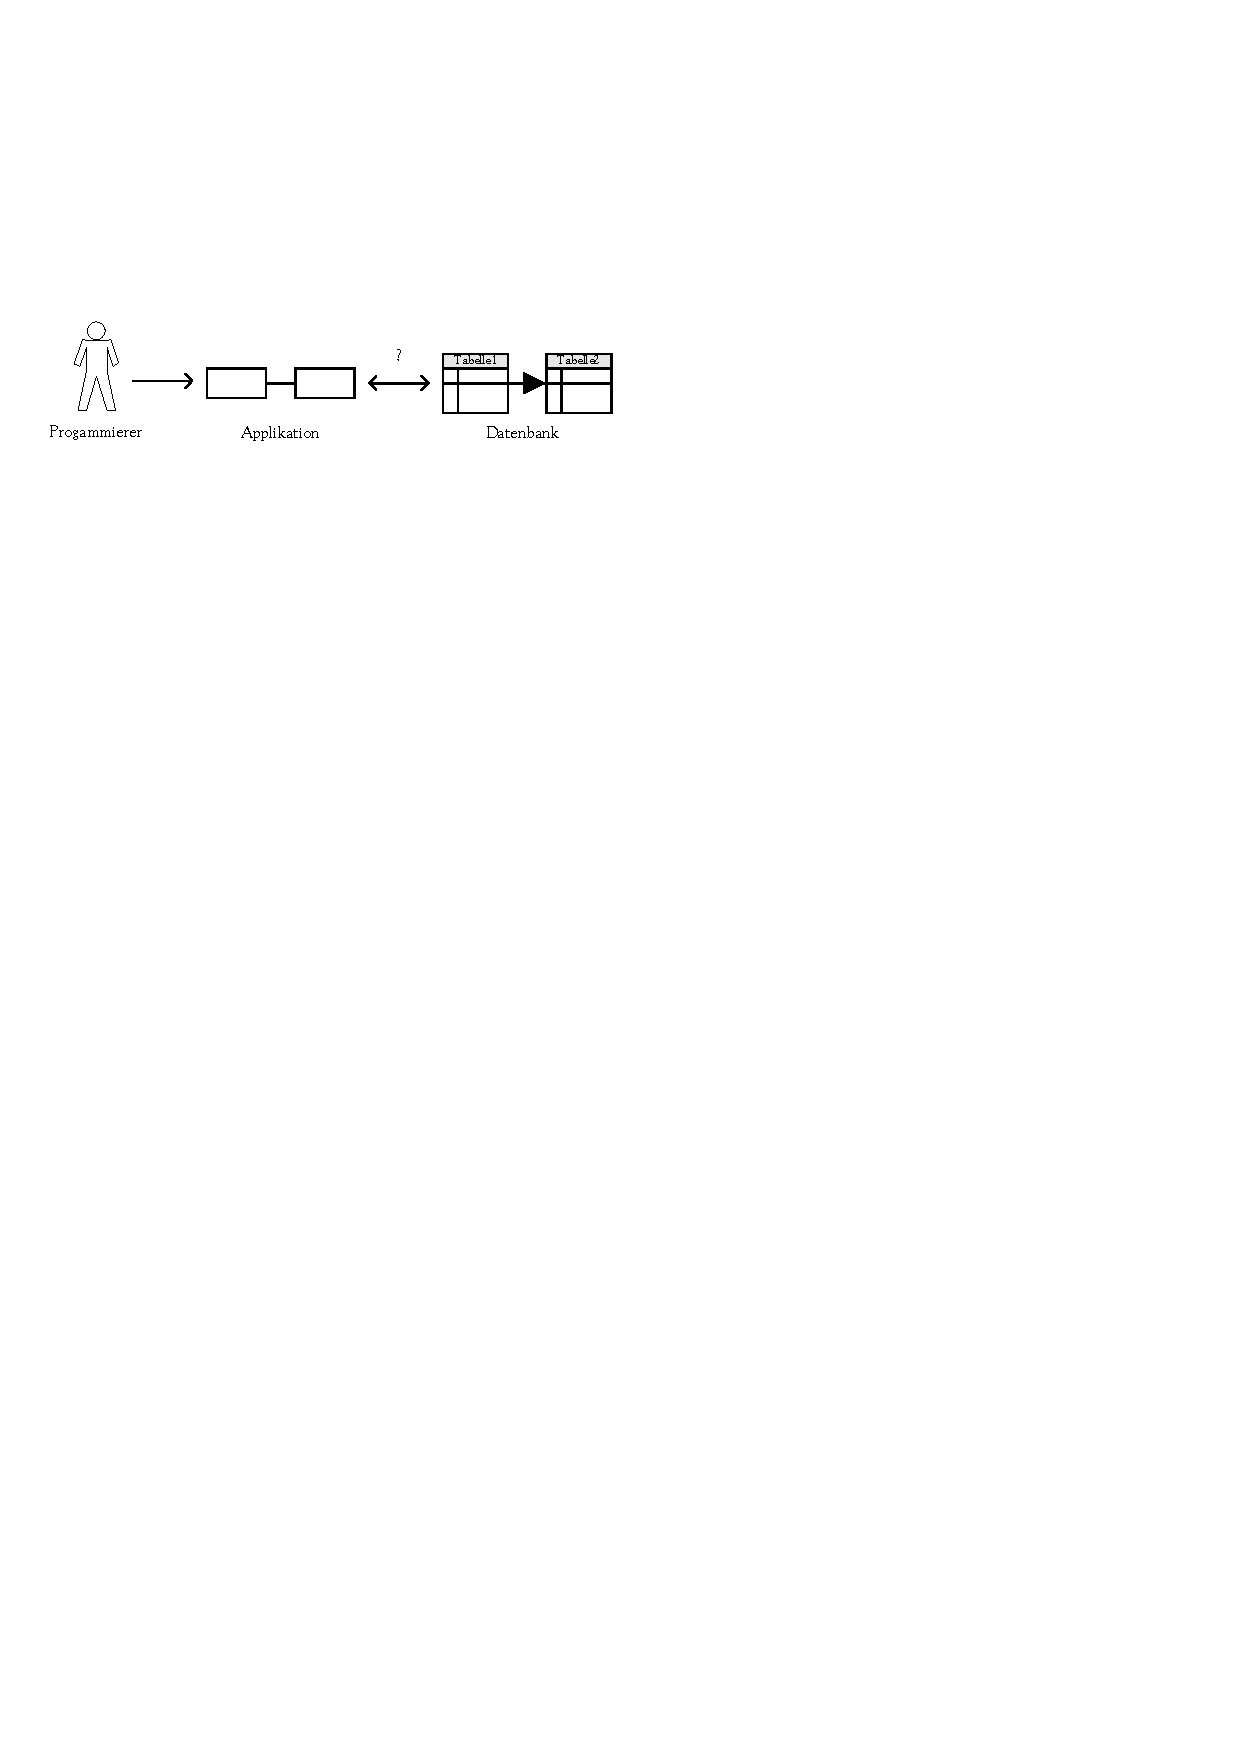
\includegraphics{./files/inc/figures/mgmtSummaryProblem}
			\caption{\label{fig:mgmtProblem}Verschiedene Strukturen bei der Applikation und der Datenbank.}
		\end{center}
	\end{figure}
 	  
\section*{Die Applikation}
	Der Name der Applikation ist \textit{S}torm 
	\textit{T}emplate-based \textit{O}bject \textit{R}elational \textit{M}apper (\textit{STORM}).
	Das Ziel von \textit{STORM} war es, ein Framework zu erstellen, das den Code f�r 
	das erw�hnte Mapping generiert. Damit wird dem Entwickler ein Teil seiner Arbeit
	abgenommen.
	
	Die Idee ist, dass der Entwickler abstrakte Domain Objekte implementiert, welche
	er mit Attributen parametrieren kann. Durch die Attributierung kann er einerseits
	das Domain Modell und andererseits das Datenbank Modell vorgeben. Anhand dieser Angaben
	wird anschliessend der gesamte Mapping Code generiert.
	Dieser Vorgang ist schematisch in Figur \ref{fig:mgmtSolution} dargestellt.
		
	
	\begin{figure}[thb]
		\begin{center}
			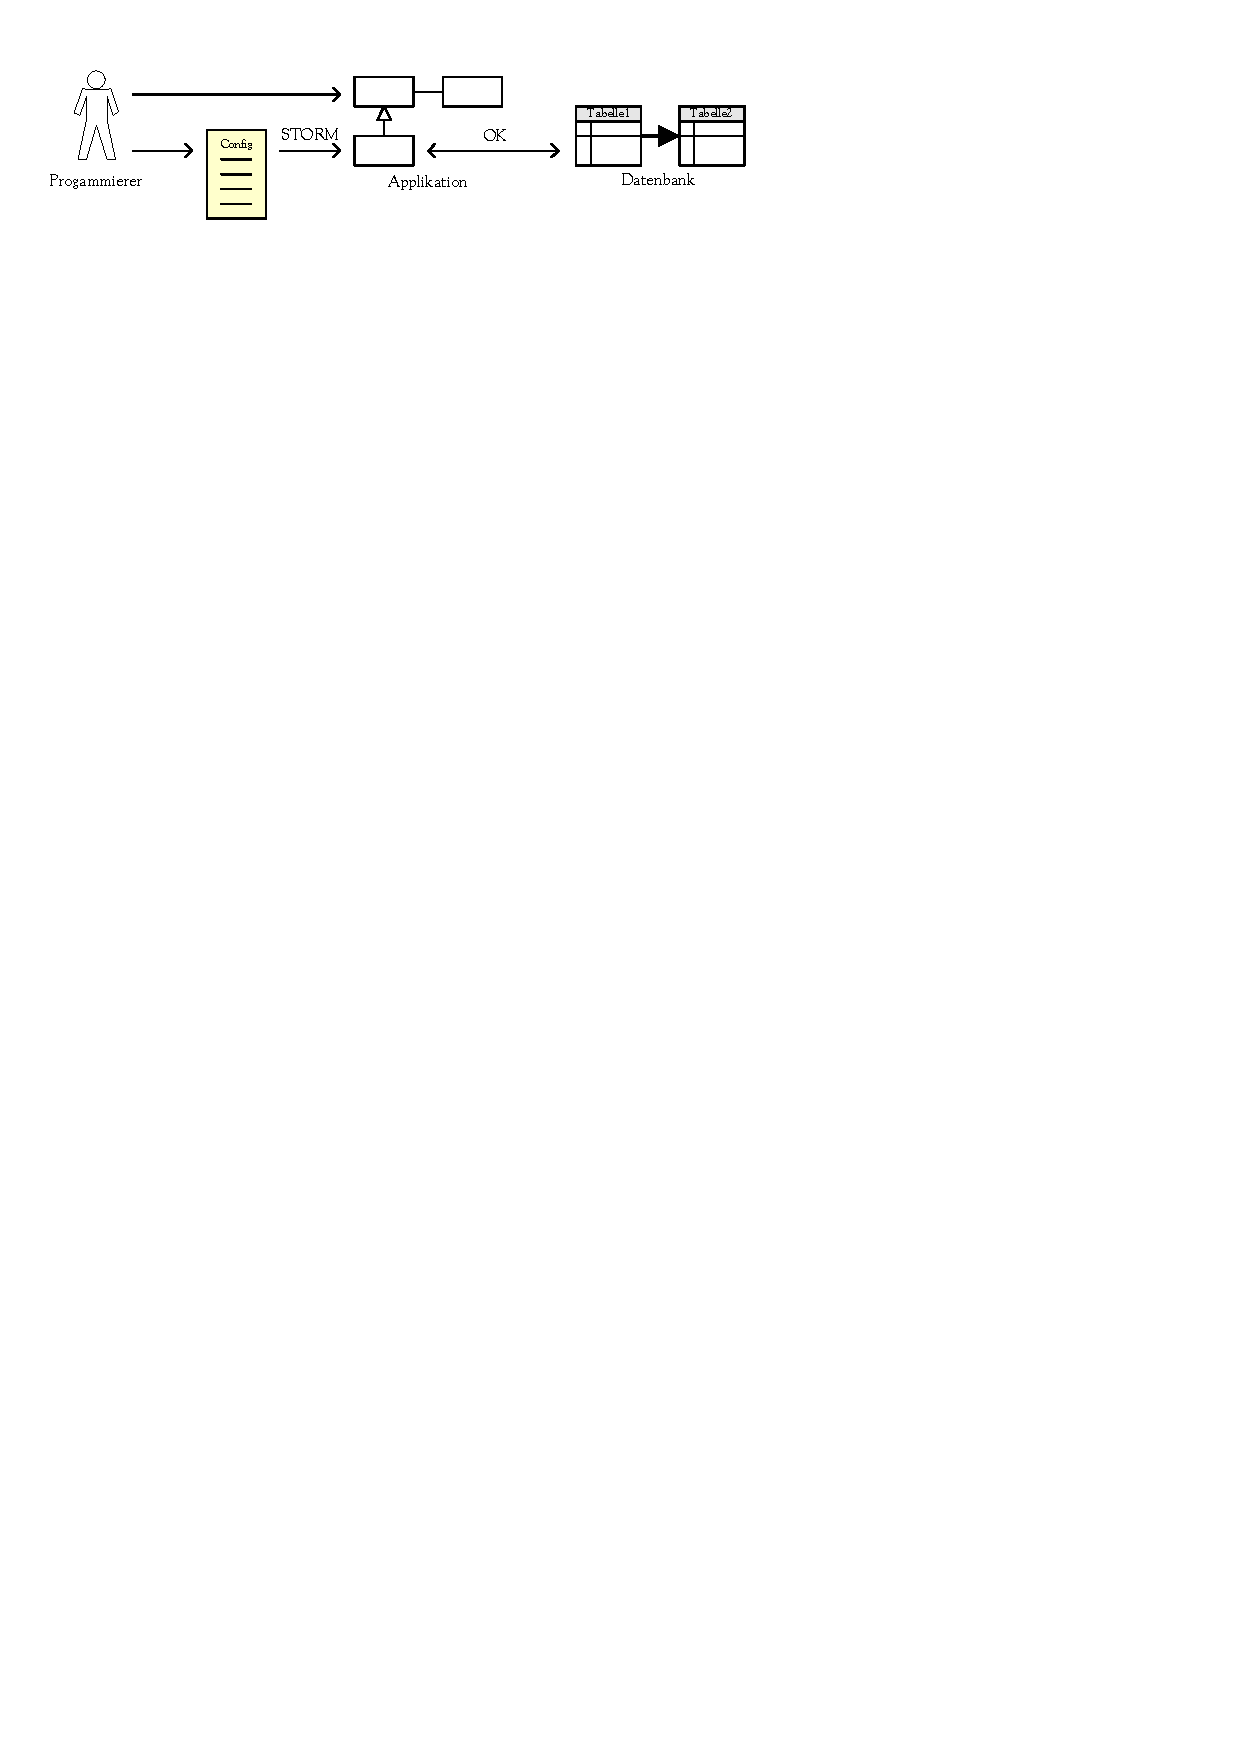
\includegraphics[width=\linewidth]{./files/inc/figures/mgmtSummarySolution}
			\caption{\label{fig:mgmtSolution}Der Code f�r das Mapping wird von \textit{STORM} erstellt. }
		\end{center}
	\end{figure}


\section*{Die Vorteile}
	Die folgende Liste gibt einen �berblick der Vorteile von \textit{STORM}.
	
	\begin{itemize}
		\item Die Entwicklungszeit einer Applikation kann stark minimiert werden.
		\item	Der generierte Mapper Code ist fehlerfrei.
		\item Der Code wird durch die Verwendung von Templates besser wartbar.
		\item Die Konfiguration wird an einem Ort, n�mlich den abstrakten Domain Objekten, vorgenommen.
		\item Der Entwickler muss sich weniger mit der Datenbank auseinandersetzen.
		\item Der Generierungsprozess ist im Visual Studio .NET eingebunden.
	\end{itemize}
	
\section*{Ausblick}
	Verschiedene Dinge konnten w�hrend dieser Arbeit nicht umgesetzt werden, da die 
	Zeit sehr begrenzt war. Daraus ergibt sich folgende Liste von Erweiterungsvorschl�gen.
		
	\begin{itemize}
		\item Meherere Locking Mechanismen werden unterst�tzt.
		\item Alle m�glichen Mapping Typen einer Datenbank werden unterst�tzt.
		\item Zus�tzlich zum Mapping zwischen Domain Objekten und Datenbank wird auch das Mapping
					zwischen Web Service Facade und Domain Objekten unterst�tzt.
		\item Als Konfigurationsm�glichkeit werden nicht nur abstrakte Klassen angeboten, sondern auch
					eine Datenbankverbindung, aus der direkt die Domain Klassen erzeugt werden.
	\end{itemize}
	
	Es w�re denkbar, die oben genannten Punkte in einer weiteren Arbeit zu implementieren. Ebenso
	m�ssten noch mehrere Testapplikationen mit \textit{STORM} entwickelt werden, um das
	Framework besser testen zu k�nnen.
	
	Die Gefahr bei der Erweiterung der jetzt bestehenden Templates ist, dass sie sehr un�bersichtlich
	werden. Man m�sste den Aufbau der Templates allenfalls �berarbeiten
	und genau planen, wie dieser aussehen m�sste, damit der Code sauber und �bersichtlich wird.
	Eine L�sung k�nnte zum Beispiel sein, ein Template in mehrere Templates aufzuteilen.
	
	Der L�sungsansatz mit den attributierten, abstrakten Klassen erscheint uns sinnvoll. 
	
	
	
	



\tableofcontents
\listoffigures
\listoftables

%%files einf�gen
\cleardoublepage
\pagenumbering{arabic}

\part{Anforderungsspezifikation}
\vspace{2cm}
	\chapter{Vision}

	\section{Ziel der Arbeit}
	\label{sec:zielDerArbeit}
		Bei den meisten Applikationen gibt es eine bestimmte Anzahl von Codezeilen,
		die repetitiven Code darstellen. Das bedeutet, dieser Code muss bei jeder
		Applikation neu geschrieben werden. Ans�tze diese
		Arbeit auf ein Minimum zu reduzieren sind generative bzw. generische Programmiertechniken.
	
		Diese Arbeit soll ein Framework zur Verf�gung stellen, mit dem repetitiver Code
		generiert werden kann. Damit wird erreicht, dass die Software besser zu Warten 
		und der Entwicklungsprozess optimiert werden kann. Die Erkenntnis aus dieser
		Arbeit soll aus dem Bericht hervorgehen und soll zeigen, wie sinnvoll ein
		generativer Ansatz ist, um einen Objekt-Relationalen Mapper zu entwickeln.
		
		Das entwickelte Framework soll m�glichst einfach zu benutzen sein. Ein wichtiger
		Aspekt der Arbeit ist dabei die Erarbeitung eines geeigneten Konzeptes f�r die
		Parametrierung der Code Generierung, damit diese m�glichst generell eingesetzt
		werden kann.
	
	\section{Positionierung}

\chapter{Detaillierte Anforderungen}
		Im Folgenden werden die Anforderungen an die Software definiert. Nicht definiert
		werden hier die �brigen Ziele, die in der Vision (\ref{sec:zielDerArbeit})
		genannt wurden.
	
		\subsection{Muss-Ziele}
			
			\begin{enumerate}
				\item Eine L�sung f�r die Konfiguration der Code Generierung muss gefunden werden.
				\item Ben�tigte Templates f�r das Tool CodeSmith
							\cite{CodeSmith} werden erstellt.
				\item Eine L�sung f�r die Integration in die Visual Studio .NET
							Umgebung wird gefunden.
				\item	Falls ben�tigt, wird ein Plugin f�r CodeSmith geschrieben.
				\item Eine �berarbeitete Version der HsrOrderApp\_S3 wird erstellt
							(mit den erstellten CodeSmith Templates) und dokumentiert. Daraus
							entsteht die HsrOrderApp\_S4.
			\end{enumerate}
		
		\subsection{Optionale Ziele}
			
			\begin{enumerate}
				\item Eine zus�tzliche Beispielapplikation zur Veranschaulichung des Nutzen der Arbeit.
				\item	Ein Wizard f�r das Visual Studio .NET, um das Erstellen der Konfigurations-Dateien
							zu erleichtern.
			\end{enumerate}
			
		Da bei dieser Arbeit ein entscheidender Teil ist, ein L�sung f�r ein Problem zu finden, k�nnen
		auch keine spezifischen, sondern nur allgemein formulierte Anforderungen aufgef�hrt werden.
		Das Problem ist, dass wir noch nicht wissen, wie diese L�sung aussehen wird und deshalb auch
		keine Anforderungen an diese L�sung stellen k�nnen. Dies entspricht auch der Aufgabenstellung.
%	\input{./files/suppSpec}
%	\input{./files/useCases}
	
\part{Analyse}
\label{par:Analysis}
\vspace{2cm}
Der folgende Teil enth�lt Kapitel in Deutsch und Englisch. Wir haben entschieden, nur den technischen Bericht in Englisch zu verfassen, hatten zu diesem Zeitpunkt jedoch schon einzelne Kapitel geschrieben.

\selectlanguage{english}
%----------
\chapter{Fundamental approach}
	Object-relation Mapping can be done in many ways. First, of course, one can implement
	the whole code by hand. As already mentioned, this is not the scope of this thesis
	and is therefore not a possible solution. Second, we have a mechanism to
	automate the coding part. In this thesis, we try to find a good solution to
	generate the code. Another approach would be to supply a set of generic
	classes, which is not our aim, either.
	
	To generate as much code as possible, we need to have information about
	the database structure as well as about the domain model and how
	to map these two. This can be quite a lot the programmer needs to
	know but usually should not be a problem. The intend of \textit{STORM} is
	to provide a programmer a solution, which allows him to specify all these
	information in a, for a programmer, natural way.
	
	The following sections describe 3 possible ways to implement such a tool
	as \textit{STORM}. The pros and cons are mentioned. There is no doubt that
	there exist more possibilities but we hope to give a reasonable overview
	with the following selection.
	
	\section{XML Schema}
		\begin{figure}[htb]
			\begin{center}
				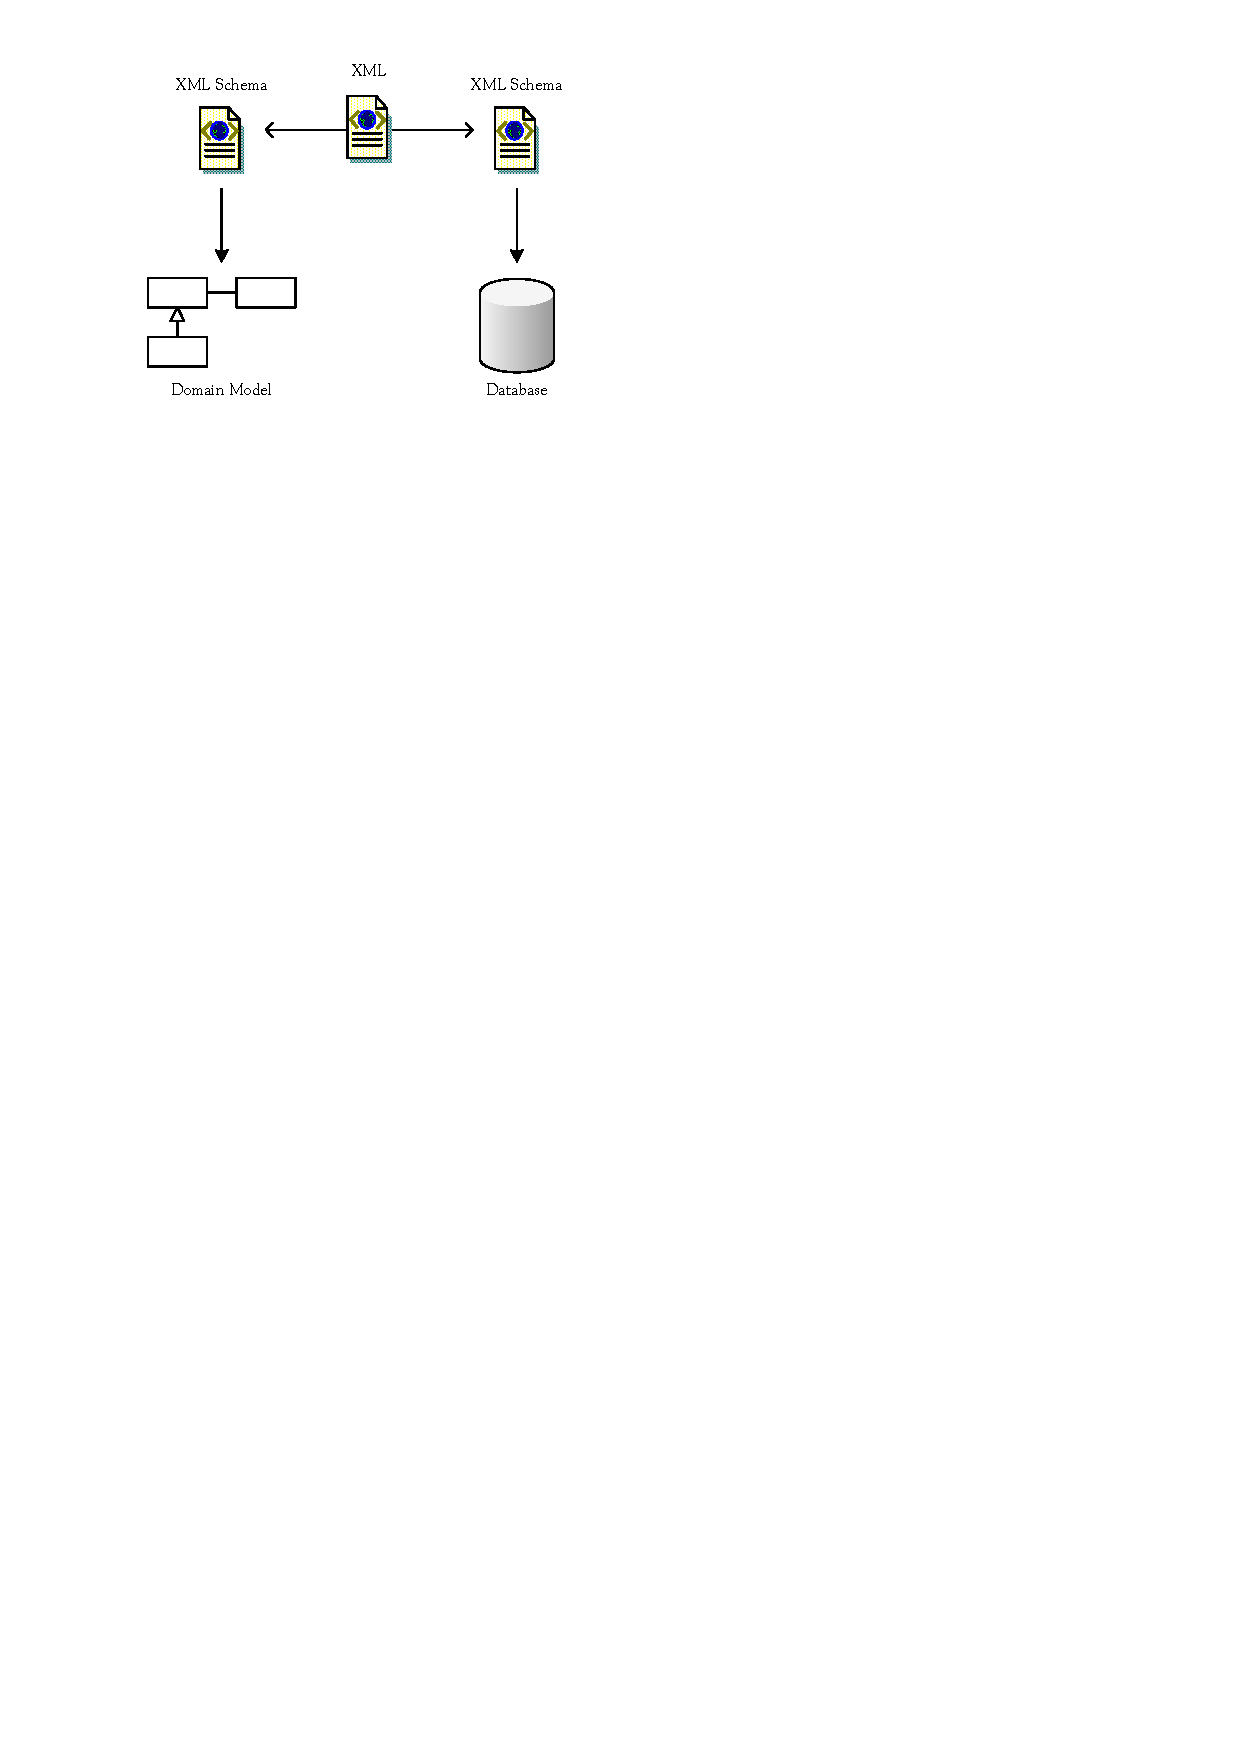
\includegraphics{./files/inc/figures/caseStudyXmlSchema}
				\caption{\label{fig:caseStudyXmlSchema} Mapping description with XML Schema}
			\end{center}
		\end{figure}
		Figure \ref{fig:caseStudyXmlSchema} shows a first possible mechanism to describe
		the information needed to generate mapping code. On the right, an XML Schema file
		is used to reflect the database structure. A sample of such a file is shown in 
		Listing \ref{lst:xsdDbConfig}. This is probably not the most sophisticated
		XML schema possible but nevertheless it is possible to describe a database structure
		with such a file. We implemented a XML schema parser which read the content of
		this file and used it as input for a CodeSmith template.
		
		The main problem with this approach is the XML schema language. It is not possible
		to describe all information needed to generate the mapping code in a schema file.
		This limitation results in the fact that another XML schema file is needed to describe
		the domain model structure (as shown on the left in Figure \ref{fig:caseStudyXmlSchema}).
		Additionally an XML file is needed to specify the mapping between the two schemes. For
		example, this XML file would include a tag describing which database table
		matches to which class in the domain model.
		
		There are a few drawbacks with this solution. One of those is that an XML schema
		is not a natural way a programmer would describe a database structure nor a 
		domain model. Another drawback is its implementation. The schema description must 
		undergo certain restrictions for consistency. A programmer therefore has to adopt
		and respect this restriction when writing a schema file. The implementation
		itself is not easy as well, because a mapping strategy needs to be defined.
		To define such a strategy which allows to specify every possible mapping is not
		an easy task.
		
		On the other hand, there are benefits which makes this approach worth looking
		at. XML schema and XML are well defined and standardised. This makes it 
		possible to delegate the task of writing the XML files to a tool such as
		a database design tool. The only thing which cannot be automated is the 
		XML file describing the mapping.
	
	\begin{lstlisting}[float,language=XML,caption=XML schema describes database structure,label=lst:xsdDbConfig]
<?xml version="1.0" encoding="utf-8" ?>
<xs:schema id="BusinessObjects1" 
		targetNamespace="http://tempuri.org/BusinessObjects1.xsd"
	elementFormDefault="qualified" 
			xmlns="http://tempuri.org/BusinessObjects1.xsd" 
			xmlns:xs="http://www.w3.org/2001/XMLSchema">
	<xs:group name="classes">
		<xs:sequence>
			<xs:element name="Person" type="PersonType" />
			<xs:element name="Address" type="AddressType" />
		</xs:sequence>
	</xs:group>
	<xs:complexType name="AddressType">
		<xs:sequence>
			<xs:element name="Person" type="PersonType" />
			<xs:element name="Street">
				<xs:simpleType>
					<xs:restriction base="xs:string">
					</xs:restriction>
				</xs:simpleType>
			</xs:element>
			<xs:element name="City">
				<xs:simpleType>
					<xs:restriction base="xs:string">
					</xs:restriction>
				</xs:simpleType>
			</xs:element>
	</xs:complexType>
</xs:schema>
	\end{lstlisting}
		
	\section{Abstract Class with Attributes}
		A second approach to describe the mapping is to write an abstract class
		with custom attributes. A code snippet of such a class is shown in Listing
		\ref{lst:abstractClass}. This class file is compiled at runtime and the custom
		attributes can be read using reflection from the resulting dll. With these attributes,
		all needed information can be retrieved.
		
		The main advantage of this is that a programmer can define everything in a single file
		rather than multiple files. Furthermore it is a more natural way for programmers because
		they are used to write classes.
		
		One could say that a drawback of attributes is that they cannot be changed at runtime.
		This is true but also, it is not required. Every information given in this 
		abstract class is static within the scope of an application. As mentioned above,
		C\# reflection mechanism is used to read the settings. This is constricted to
		the process of generating code. The generated code does not make use of reflection. This
		would be possible but would result in a poorer performance.
		
		From our point of view, this approach is the most feasible.
	
	
	\begin{lstlisting}[float,language={[Sharp]C},caption=Abstract class with custom attributes,label=lst:abstractClass]
[Table("Addresses", true),
VersionField("chTimeStamp", typeof(Timestamp))]
public abstract class Address : DomainObject
{
	[Column("AddressID"),
		PrimaryKey]
	public abstract int AddressId {get; set;}

	[Column("City")]
	public abstract string City {get; set;}

	[Column("Street")]
	public abstract string Street {get; set;}
}
	\end{lstlisting}
	
	\section{Extended C\# Compiler}
		This is the most advanced approach and would give the highest possible flexibility. The
		basic idea is to take an existing C\# compiler and extend it to work with custom defined
		keywords. With this new introduced keywords, the mapping information could be given in a
		well defined, familiar manner.
		
		Due to the limited time for this thesis, we do not follow this approach in more detail, 
		although it would be very interesting and promising. A possible solution could be to
		use a compiler generation tool such as Coco/R \cite{Coco/R}.
			
\selectlanguage{ngerman}
\chapter{Konzeptionelles Modell}

	\section{Generisch vs. generativ}
		Zuerst muss entschieden werden, welche Teile des Codes generiert werden k�nnen und bei 
		welchen Teilen ein generativer Ansatz besser ist. Um mit der HsrOrderApp\_S3 als Vorlage m�glichst 
		bald eine lauff�hige HsrOrderApp\_S4 mit generiertem Code zu erhalten, werden wir uns 
		auf die Generierung von Domain Objekt Klassen und Mapper Klassen beschr�nken.

		Die Beschreibungen f�r die Generierung des Codes werden in abstrakten Klassen gemacht.		
		
		Da UnitOfWork, Identity Map und einige Finder Methoden noch generisch implementiert werden,
		ist es n�tig, dass die Domain Objekte von einer gemeinsamen Oberklasse abgeleitet werden.
		Die Klasse \verb~DomainObject~ ist Teil der \textit{STORM} Library. Die abstrakten Klassen m�ssen 
		von dieser abgeleitet werden.
		
		\begin{figure}[hbt]
			\begin{center}
				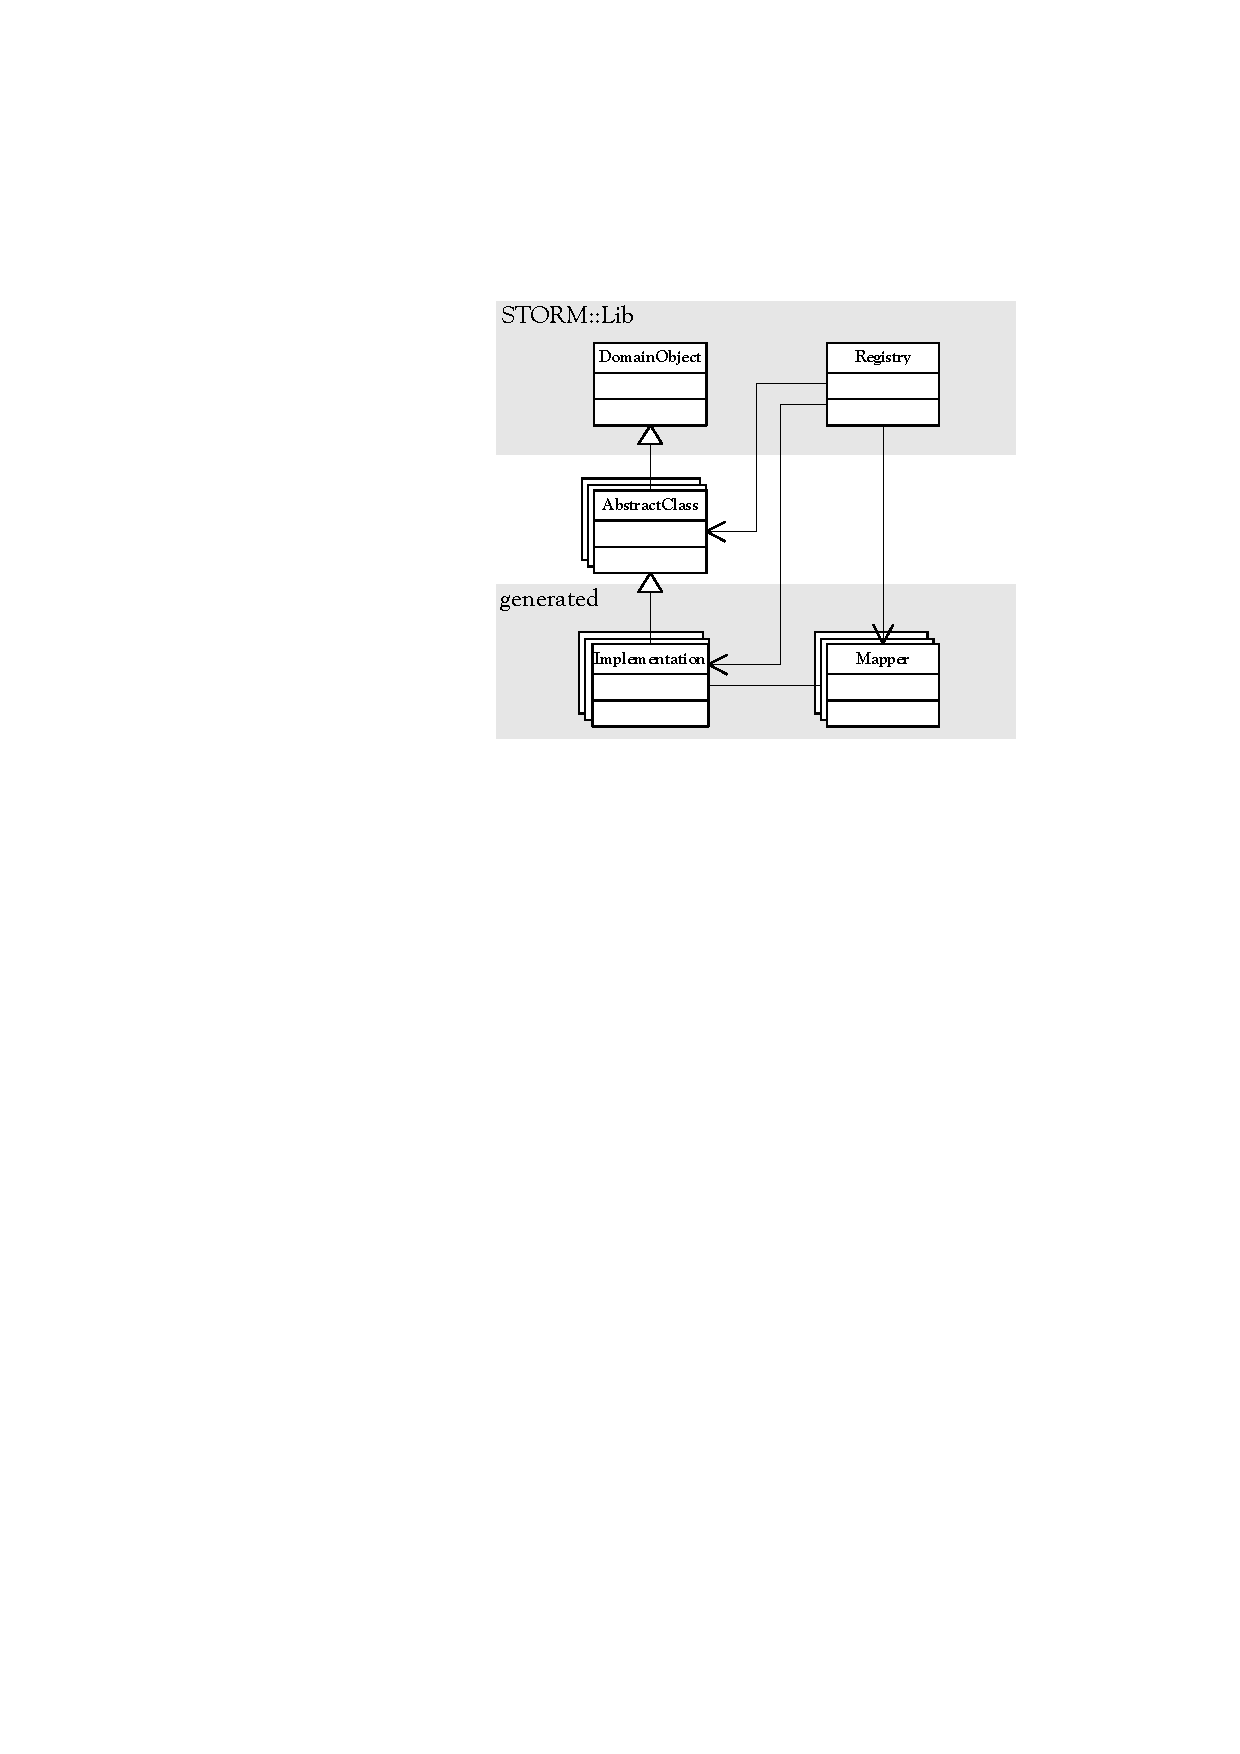
\includegraphics{./files/inc/figures/AnalysisKonzept1}
				\caption{\label{fig:AnalysisKonzept1} Vererbungsstruktur mit STORM}
			\end{center}
		\end{figure}
		
		Die Abbildung \ref{fig:AnalysisKonzept1} zeigt die Vererbungsstruktur vom einem \verb~DomainObject~ bis zur generierten 
		Implementation.
	
		Ein Problem, das gel�st werden muss, ist das Arbeiten mit den generierten Implementationen. Weder aus dem 
		selber geschriebenen Code noch aus anderen generierten Klassen, darf auf generierte Klassen 
		zugegriffen werden. Denn der Code muss auch kompilierbar sein, wenn noch kein oder nur ein Teil des Codes 
		generiert wurde.
		
		Damit jedoch der generierte Code auch genutzt werden kann, muss dieser an einer zentralen Stelle verwaltet werden.
		Hier kommt die Registry zum Einsatz.
				
	\section{Registry}
		
		Die generierten Klassen werden mit Attributen versehen. Wenn die Applikation gestartet wird, muss eine 
		Init Funktion der Registry aufgerufen werden, die den gesamten Code per Reflection analysiert und die 
		Implementationen der Domain Objekte sowie die dazugeh�rigen Mapper sucht und in einer Tabelle ablegt.
		
		Die nachfolgend beschriebenen Factory und Finder Klassen k�nnen von der Registry �ber ein statisches 
		Attribut in der Implementation geholt werden.
		
	\section{Factory}
	\label{sec:analyseFactory}
		Soll zum Beispiel ein Objekt der Implementation \verb~PersonImpl~ erstellt werden, muss zuerst von der Registry 
		mit dem abstrakten Typ \verb~Person~ dessen Factory geholt werden. Wie in Abbildung \ref{fig:AnalysisKonzept2} 
		gezeigt, ist die Factory eine interne Klasse der Implementation. Sie kann somit den Implementations Code 
		instanzieren, da er auf jeden Fall existiert. 
		
		Die generierte Factory stellt Standard Methoden zur Verf�gung. Diese werden aus dem selber geschriebenen Code    
		�ber das Interface IFactory aufgerufen.
		
		In der abstrakten Klasse k�nnen bei Bedarf zus�tzliche Factory Methoden beschrieben werden, die im generierten 
		Code implementiert werden. Die Beschreibung geschieht mit Attributen.
		
		\begin{figure}[hbt]
			\begin{center}
				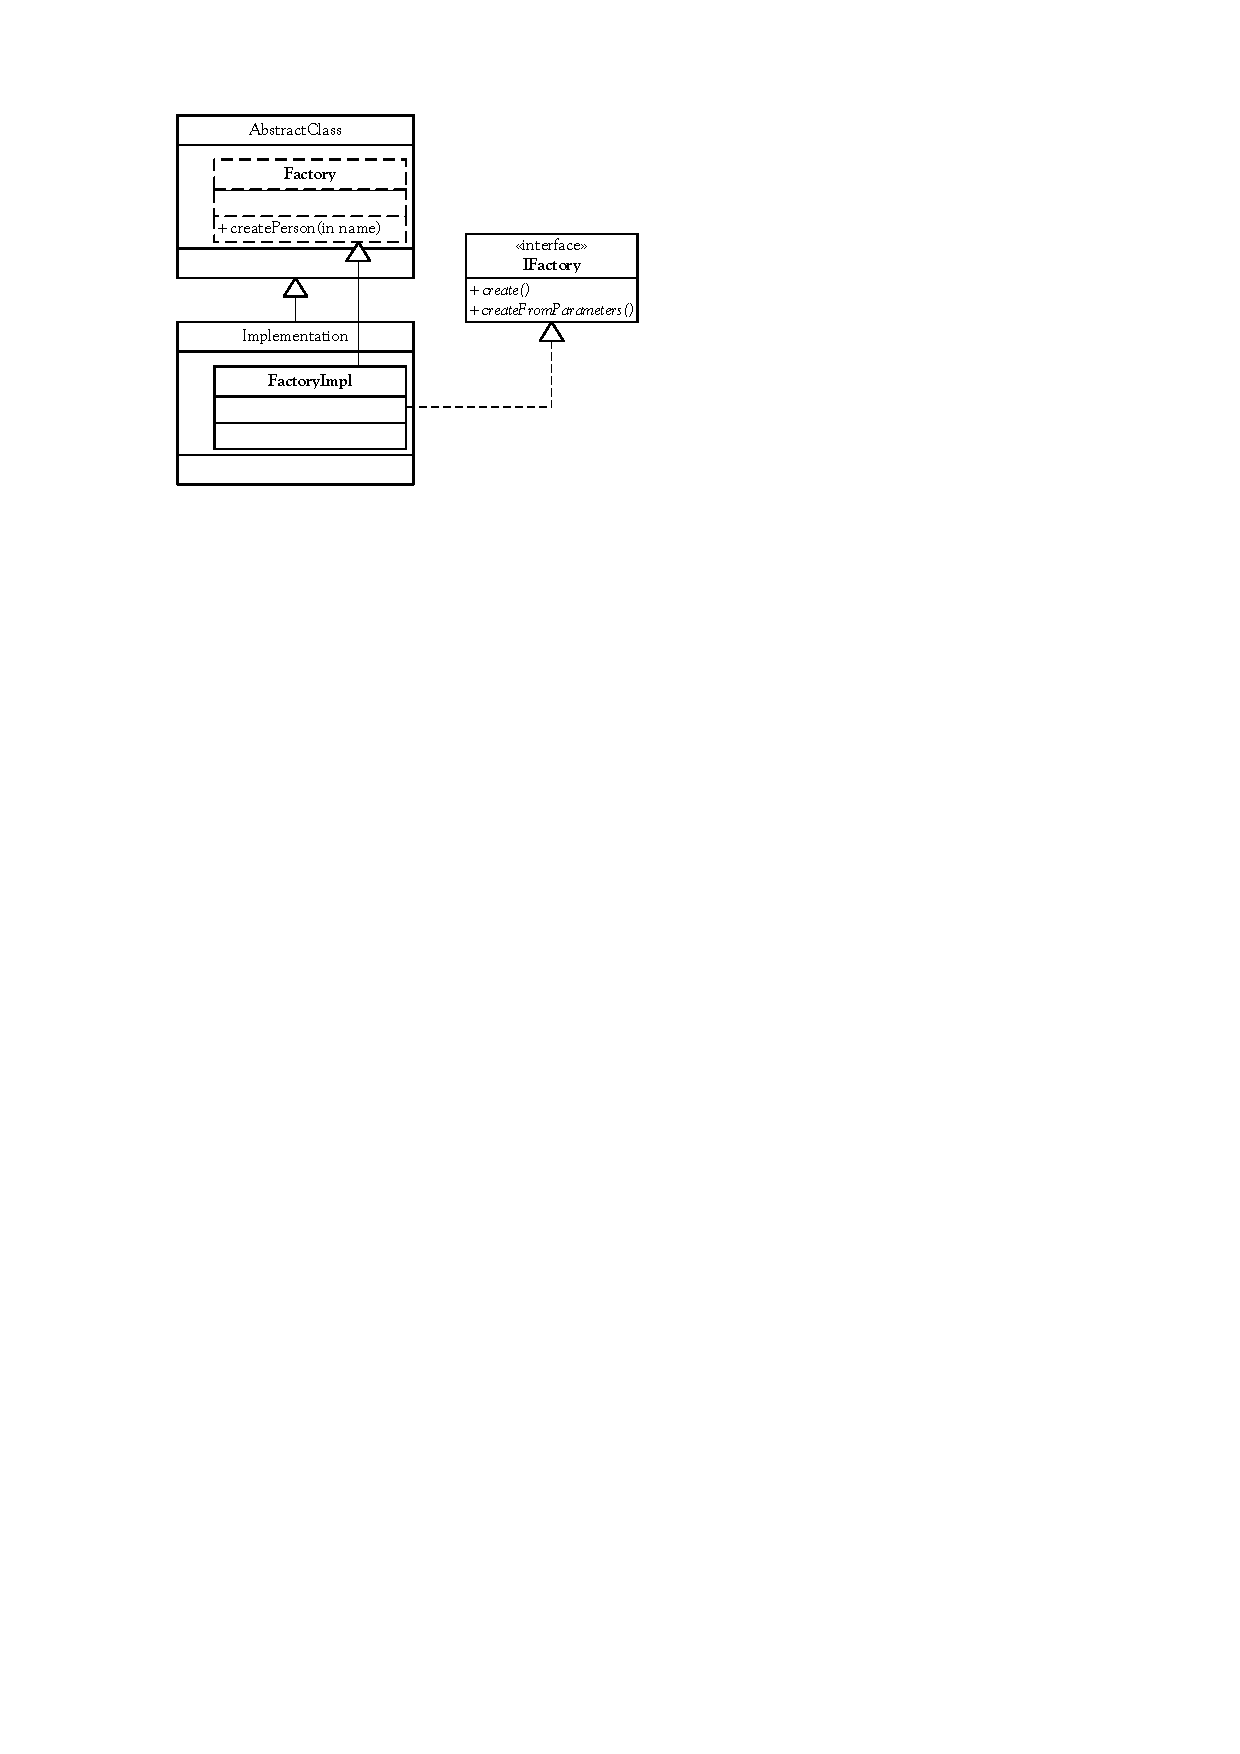
\includegraphics{./files/inc/figures/AnalysisKonzept2}
				\caption{\label{fig:AnalysisKonzept2} Business Objekt mit interner Factory Klasse}
			\end{center}
		\end{figure}
	
		
	\section{Finder}
	\label{sec:analyseFinder}
		Will man ein Objekt in der Datenbank suchen, muss man auf sogenannte Finder Methoden zugreifen k�nnen. Da diese
		Funktionen generiert werden, stehen wir vor dem gleichen Problem wie bei der Factory. Wie man in Abbildung
		\ref{fig:AnalysisKonzept3} sehen kann, werden die Finder Klassen ebenfalls als interne Klassen realisiert. 
		Die drei Standard Finder Methoden k�nnen �ber das Interface IFinder aufgerufen werden.
		
		In der abstrakten Klasse k�nnen wie bei der Factory zus�tzliche Finder Methoden beschrieben werden.
						
		\begin{figure}[hbt]
			\begin{center}
				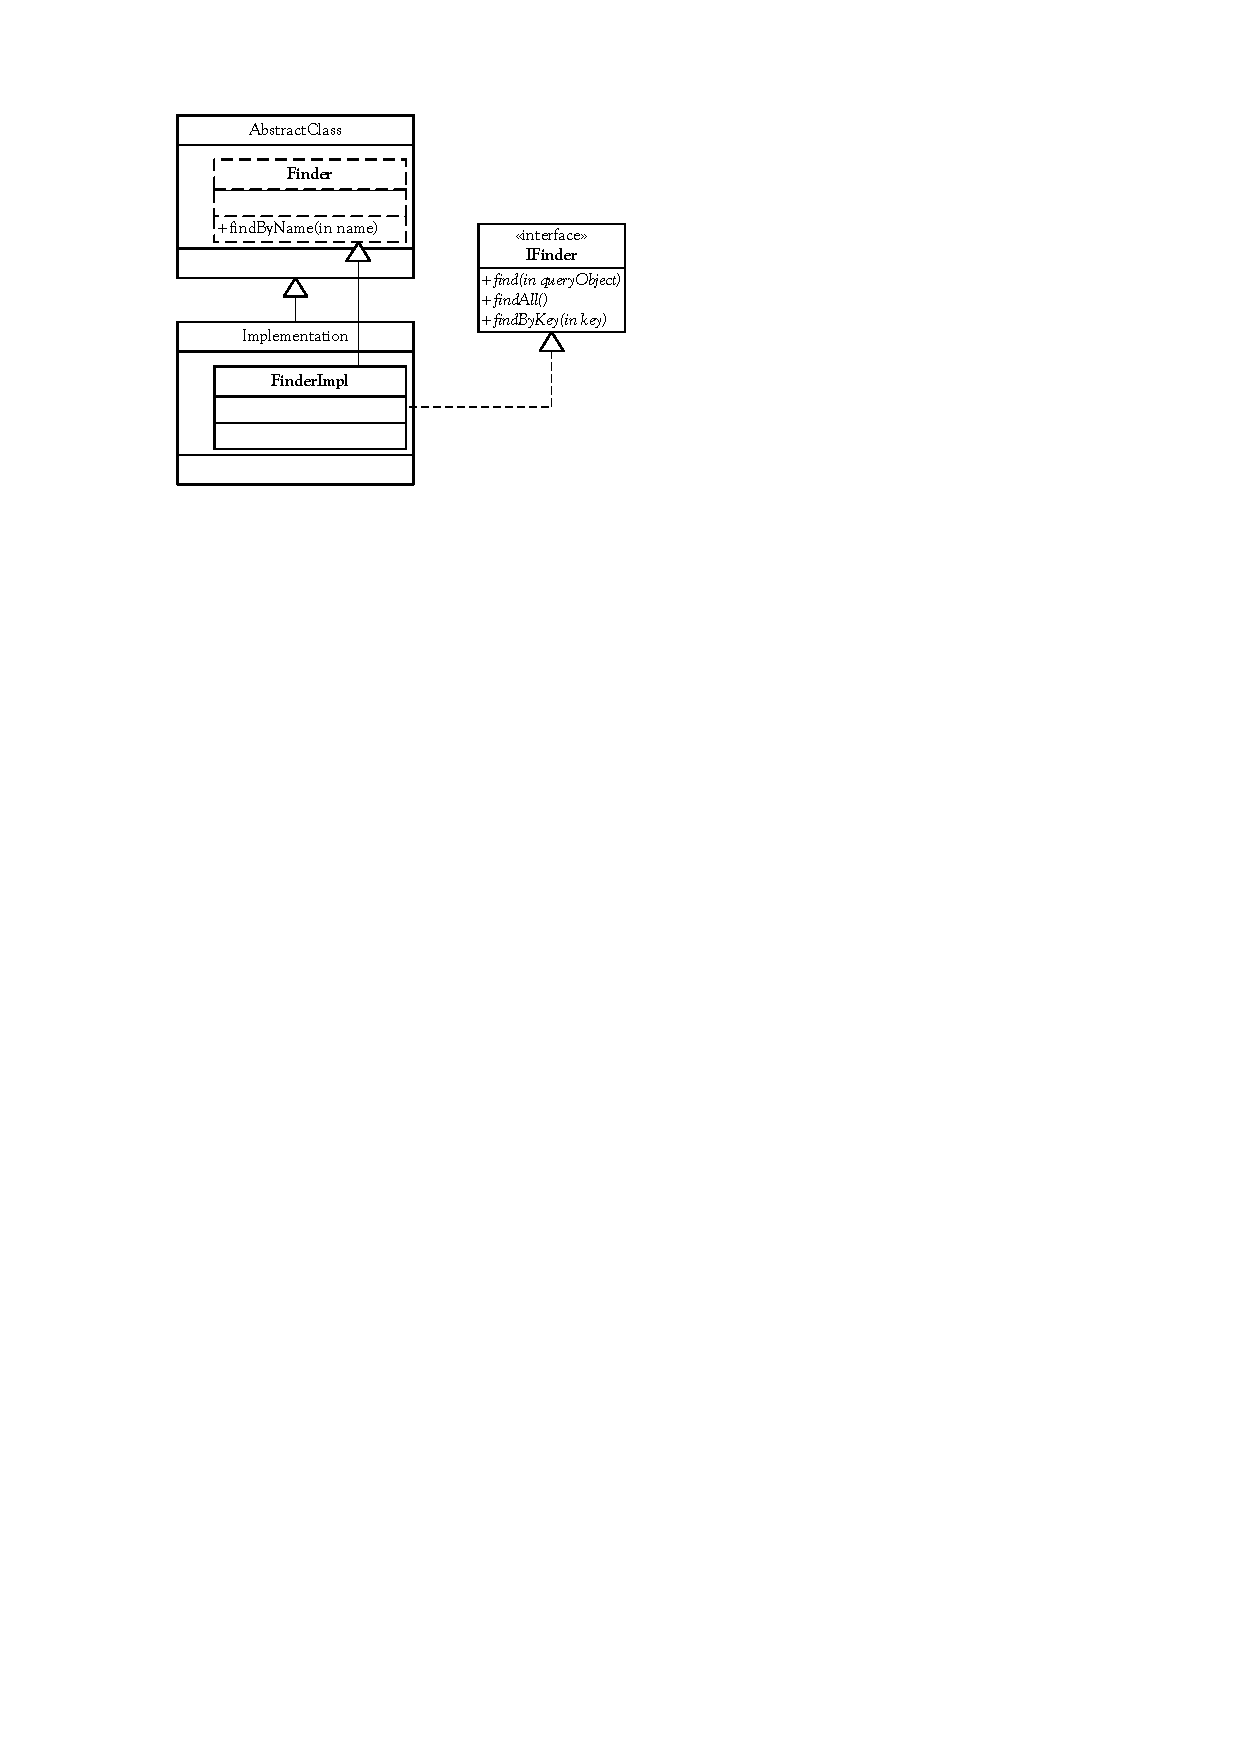
\includegraphics{./files/inc/figures/AnalysisKonzept3}
				\caption{\label{fig:AnalysisKonzept3} Business Objekt mit interner Finder Klasse}
			\end{center}
		\end{figure}
	
		Die Methode \verb~findAll()~ gibt eine Liste mit allen Objekten von einem bestimmten Typ zur�ck. \verb~findByKey()~
		sucht ein Objekt mit dem gew�nschten eindeutigen Schl�ssel. Der Methode \verb~find()~ kann ein QueryObject mitgegeben 
		werden, das Bedingungen f�r die Suche auf der Datenbanken speichert.
		
	\section{HsrOrderApp\_S4}
	
		Das Design der HsrOrderApp\_S4 wird vor allem durch die existierende Datenbank vorgegeben. 
		Das Modell der HsrOrderApp\_S3 wird wo m�glich �ber\-nommen. Eine der markantesten �nderungen 
		ist, dass die Domain Objekte in abstrakte Klassen und generierte Implementationen davon aufgeteilt 
		werden. Diese sind im konzeptionellen Modell auf der n�chsten Seite rot (abstrakt) und gr�n (generiert).
		
		Da sowieso alle Domain Objekte von der Oberklasse \verb~DomainObject~ abgeleitet werden m�ssen, 
		haben wir entschieden den Primary Key (Klasse \verb~Key~) und das Versions Feld (Klasse 
		\verb~Timestamp~) in die DomainObject Klasse auszulagern anstatt in die Implementationen zu generieren.
		Dies ist auch eine Erleichterung f�r den Programmierer, da er sie nicht in den abstrakten Klassen
		auff�hren muss.
		
		Das konzeptionelle Modell auf der n�chsten Seite zeigt bei den Domain Objekten die internen Factory 
		und Finder Klassen. Diese sind in den Abschnitten \ref{sec:analyseFactory} und \ref{sec:analyseFinder} 
		beschrieben.
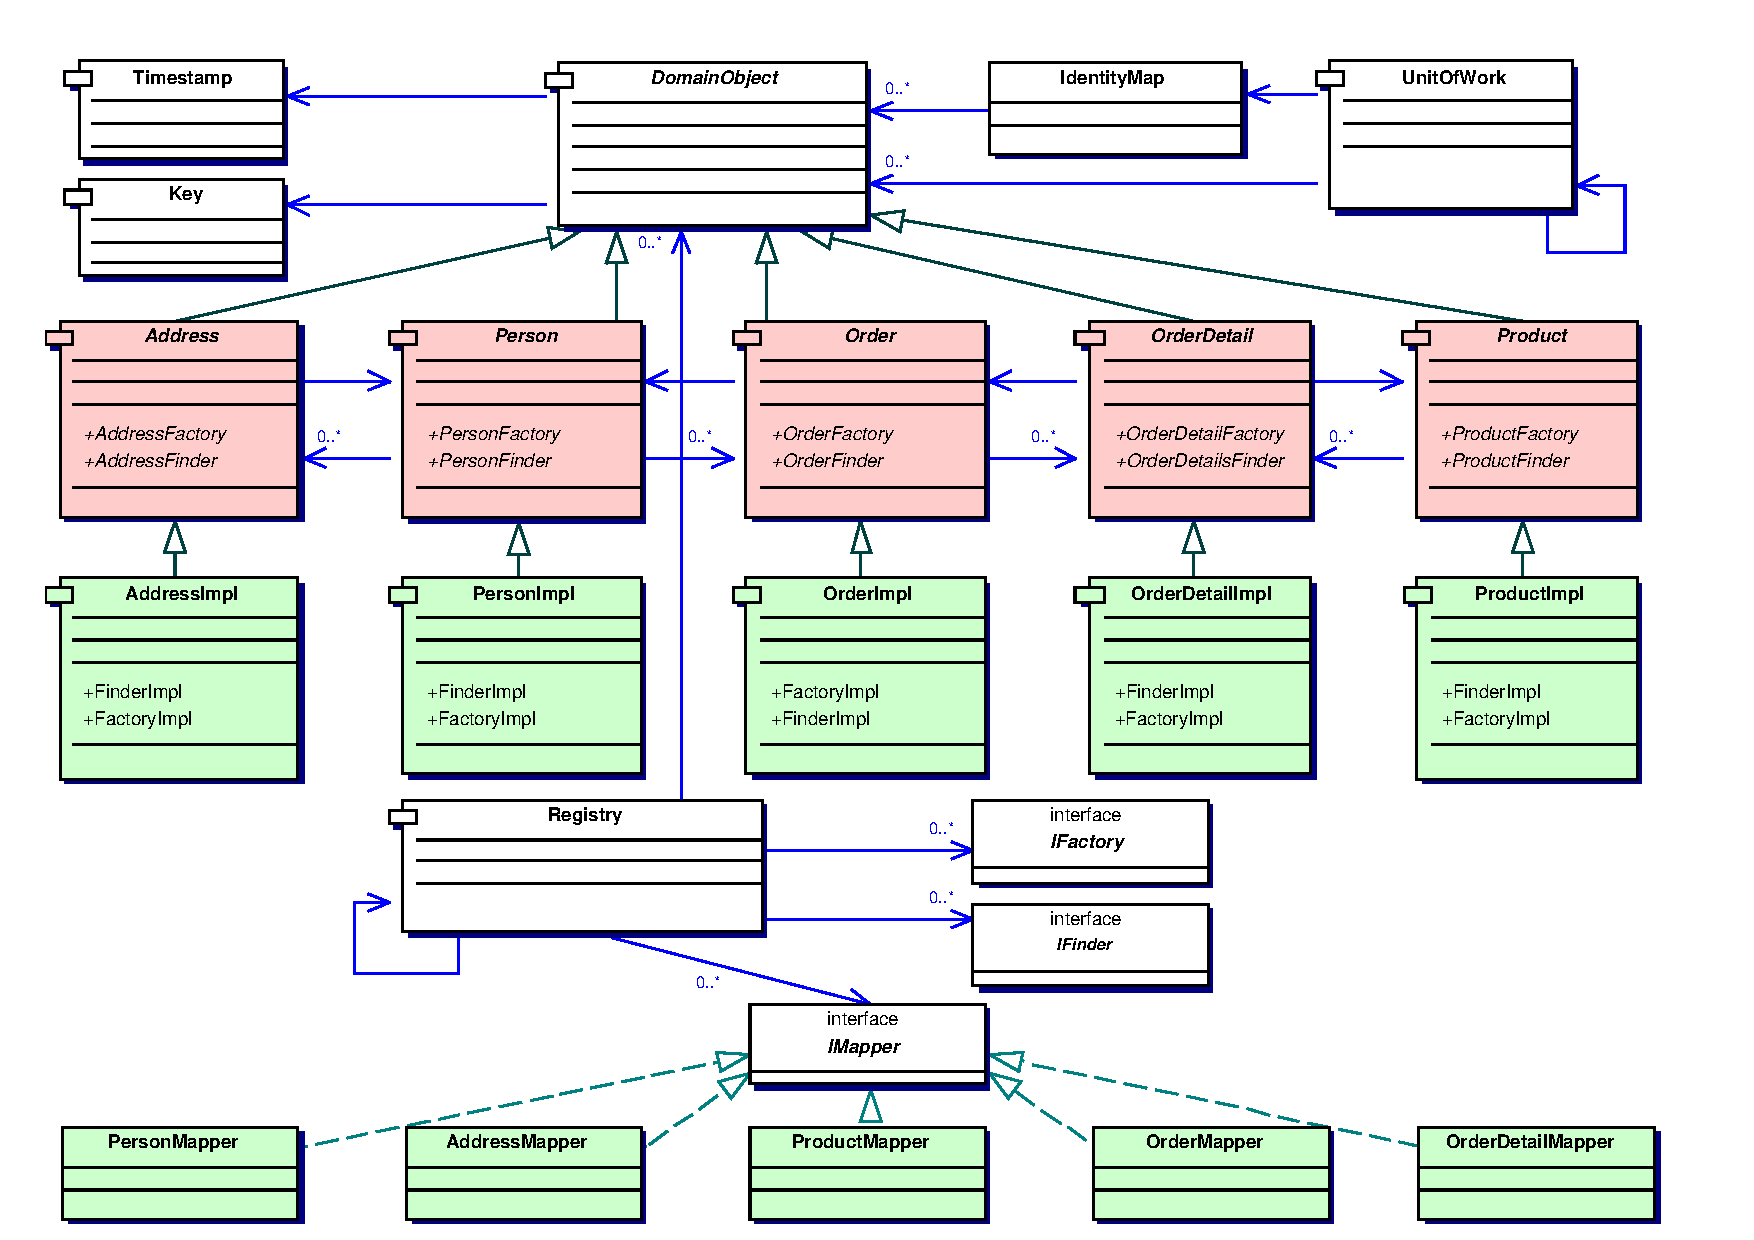
\includepdf[pages={1},landscape]{./files/inc/figures/AnalyseKonzeptionellesModell}

\selectlanguage{english}
\chapter{Enumeration Mapping}
\label{cha:enumerations}

	While the mapping of common data types is mostly clear we have to 
	take a special look to enumerations. Enumeration is a type where 
	numeric constants are represented by alphanumeric keywords or even 
	descriptions. For developers the enum data type is a way to make 
	the source code more readable. But most databases do not provide 
	this type.

	%-----
	\section{Enum data type}
		The enum data type has values given at compile time. If you want 
		to change the values it is needed to recompile the code. Independent 
		from how the mapping to the database is done there will ever be 
		the problem of assuring the database consistency.
		
		An object state 
		like shown in Listing \ref{lst:enumObjectState} is a place where 
		enumeration makes really sense, because it makes the code much 
		more readable.
		
		\begin{lstlisting}[float=hbt,language={[Sharp]C},caption=Object state with enumeration,label=lst:enumObjectState]
public class DomainObject
{
	public enum ObjectState {Unchanged, Modified, Added, Deleted, Detached}

	private ObjectState m_state = ObjectState.Detached;

	internal ObjectState State     
	{
		get { return m_state; }
		set { m_state = value; }
	}
}
		\end{lstlisting}
		
		If you don't want to run into problem you should use enumerators only 
		for internal purposes never mapped to the database.	Also the user of a 
		program should never see any values of an enum.


	\section{Current mapping}
	
		The existing HsrOrderApp uses the enum type for a person role. In Figure
		\ref{fig:AnalysisEnumOld}	you can see the PersonRole table mapping PersonIDs 
		to a RoleName. The value of the enum is written to the database as a string
		for each assignment. 
		
		\begin{figure}[hbt]
			\begin{center}
				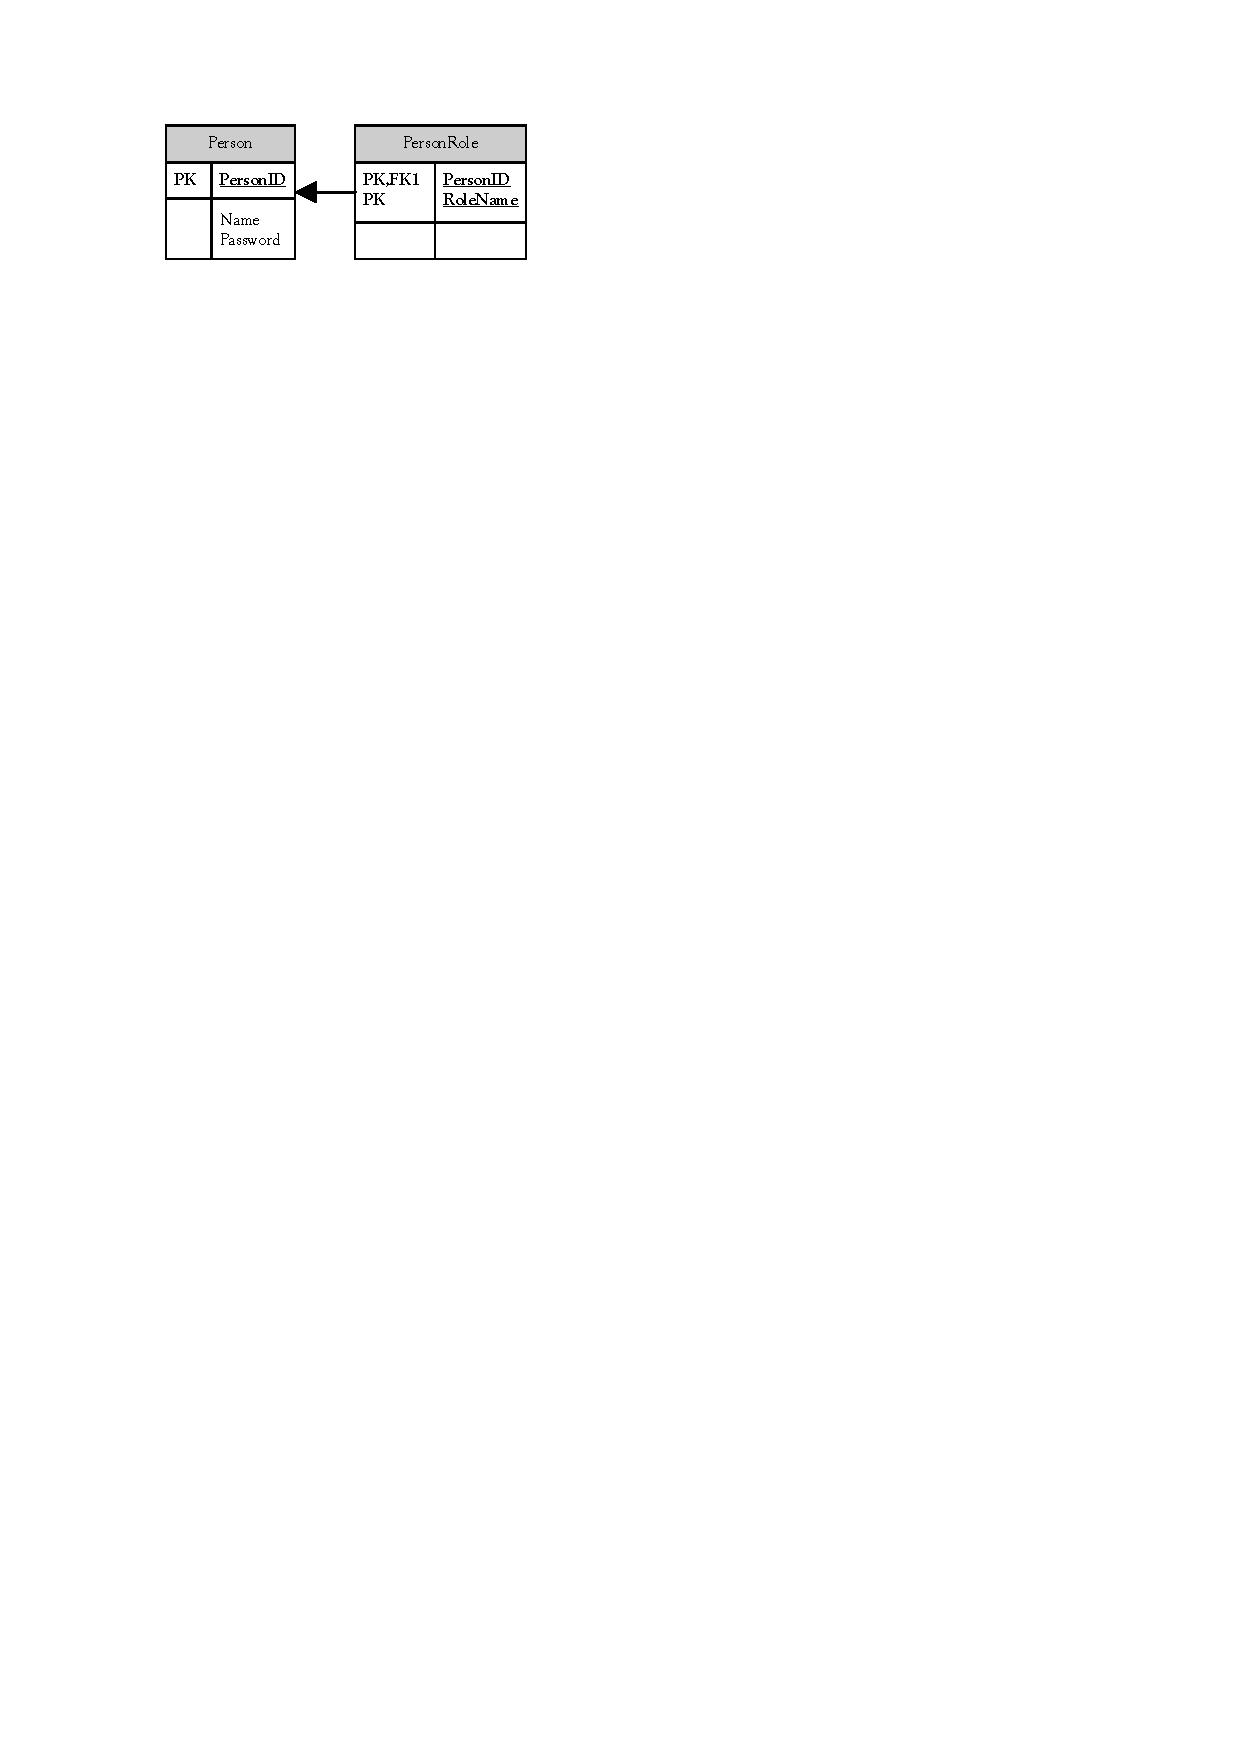
\includegraphics{./files/inc/figures/AnalysisEnumOld}
				\caption{\label{fig:AnalysisEnumOld} existing database}
			\end{center}
		\end{figure}
		
		This is a bad database design because the strings are saved redundant. But not
		only that. You will also run into big troubles if you want to add, change or delete
		values of the enumerator. Every change must be done in the code and on the database 
		to assure the consistency between enum values and database entries.
		
	%-----
	\section{Normalized design}
	
		In a fully normalized database each string should be only saved once 
		referenced by a unique id like you can see in Figure \ref{fig:AnalysisEnumNew}. 
		There every role description exists exactly once. The table PersonRole now 
		only maps RoleIDs to PersonIDs.

		\begin{figure}[hbt]
			\begin{center}
				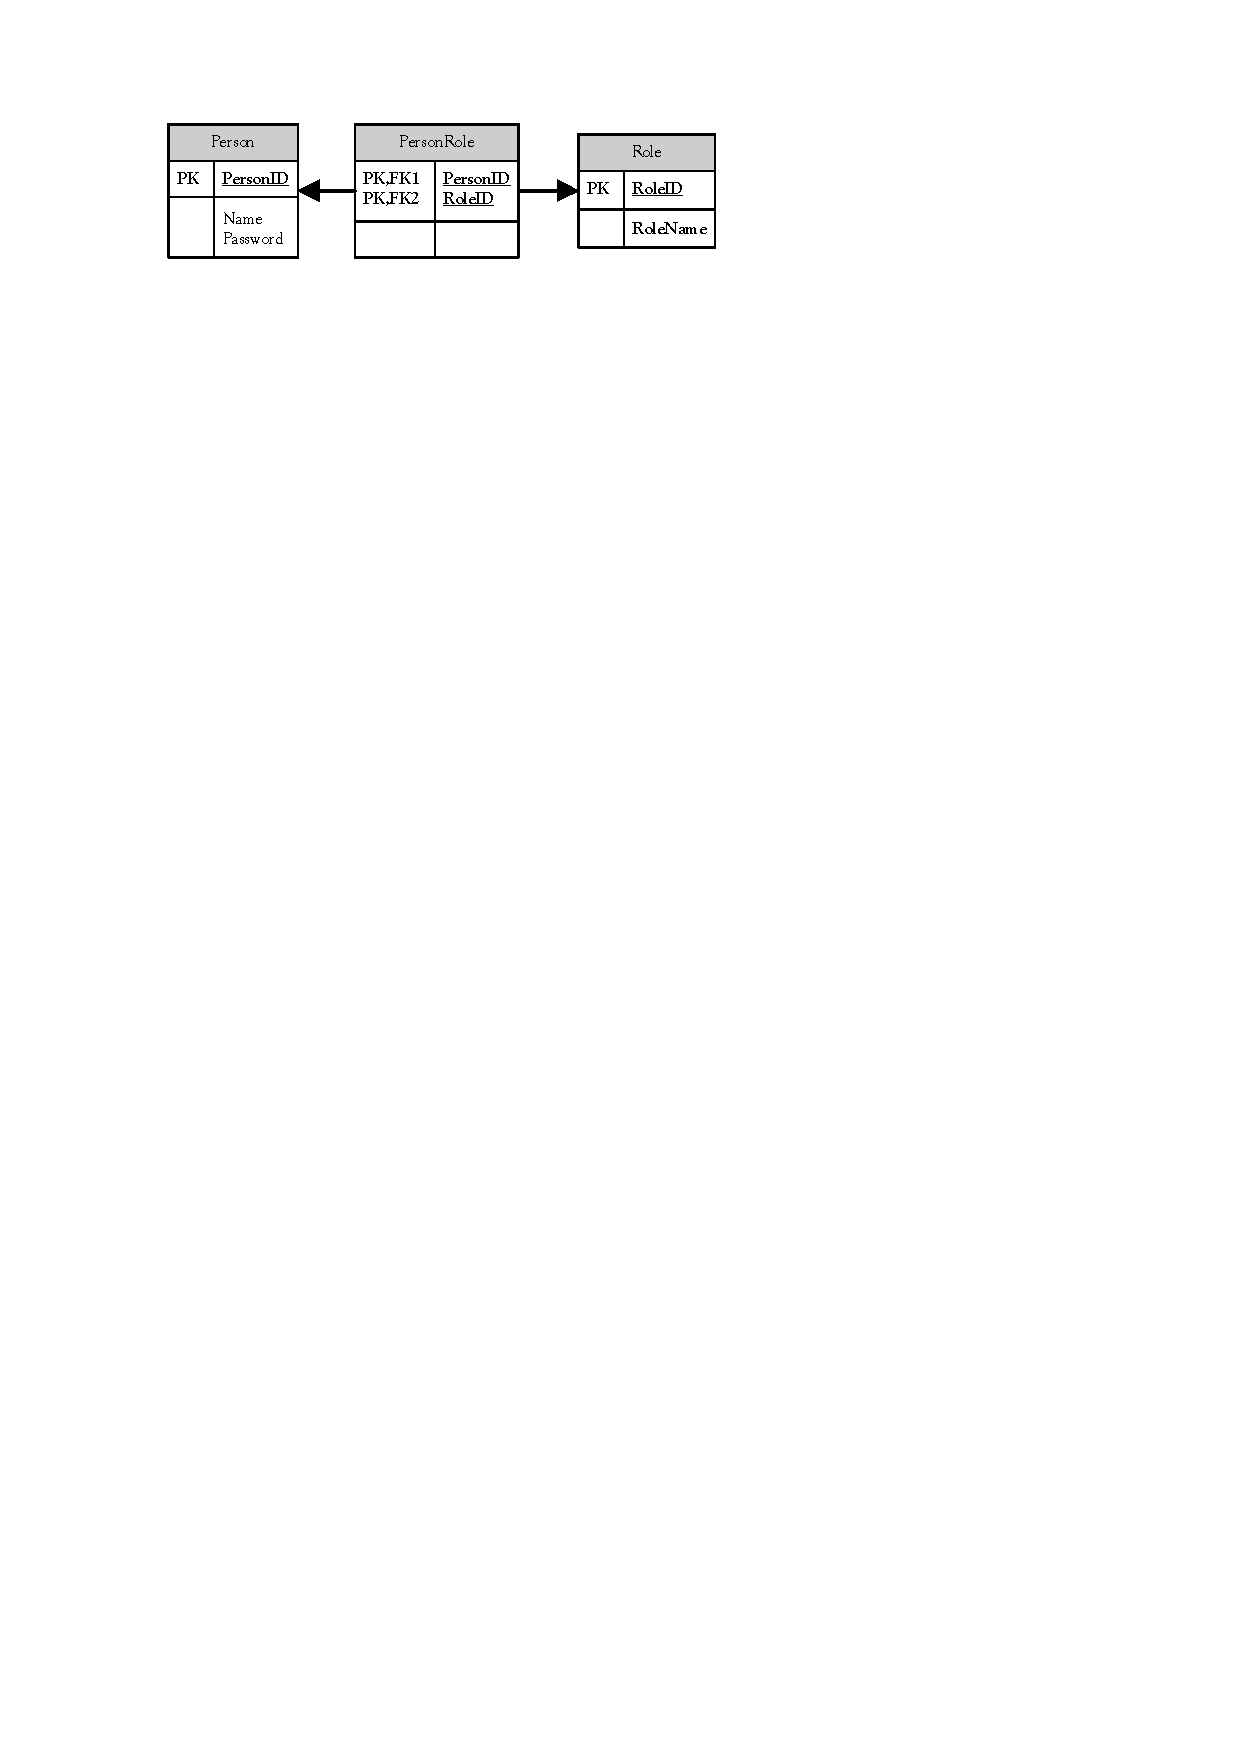
\includegraphics{./files/inc/figures/AnalysisEnumNew}
				\caption{\label{fig:AnalysisEnumNew} normalized database}
			\end{center}
		\end{figure}
	
	
	%-----
	\section{Lookup tables}

		An enum is not dedicated to present a description to the user. Every text 
		representing a database entry has to come out of the database. So you can 
		avoid consistency problem between code and database.
		
		Descriptions for numeric ids are always references to so called lookup 
		table. You can add all descriptions to one table or use one tables for each 
		relation. With a little effort it is even possible to save the values in 
		different languages.
				
		To change, add and remove the values you don't have to recompile the code 
		but only change the entries in the database. Another advantage of a lookup 
		table is the flexibility of such a table. 
		
		In Figure \ref{fig:AnalysisEnumExtended} you can see two tables which has 
		its descriptions in the same table. The table Car has the names of colors 
		and the table PersonRole its role names in the EnumLookup table. This 
		descriptions can be added for different languages. The names of languages 
		are defined in the Language table.
		
		\begin{figure}[hbt]
			\begin{center}
				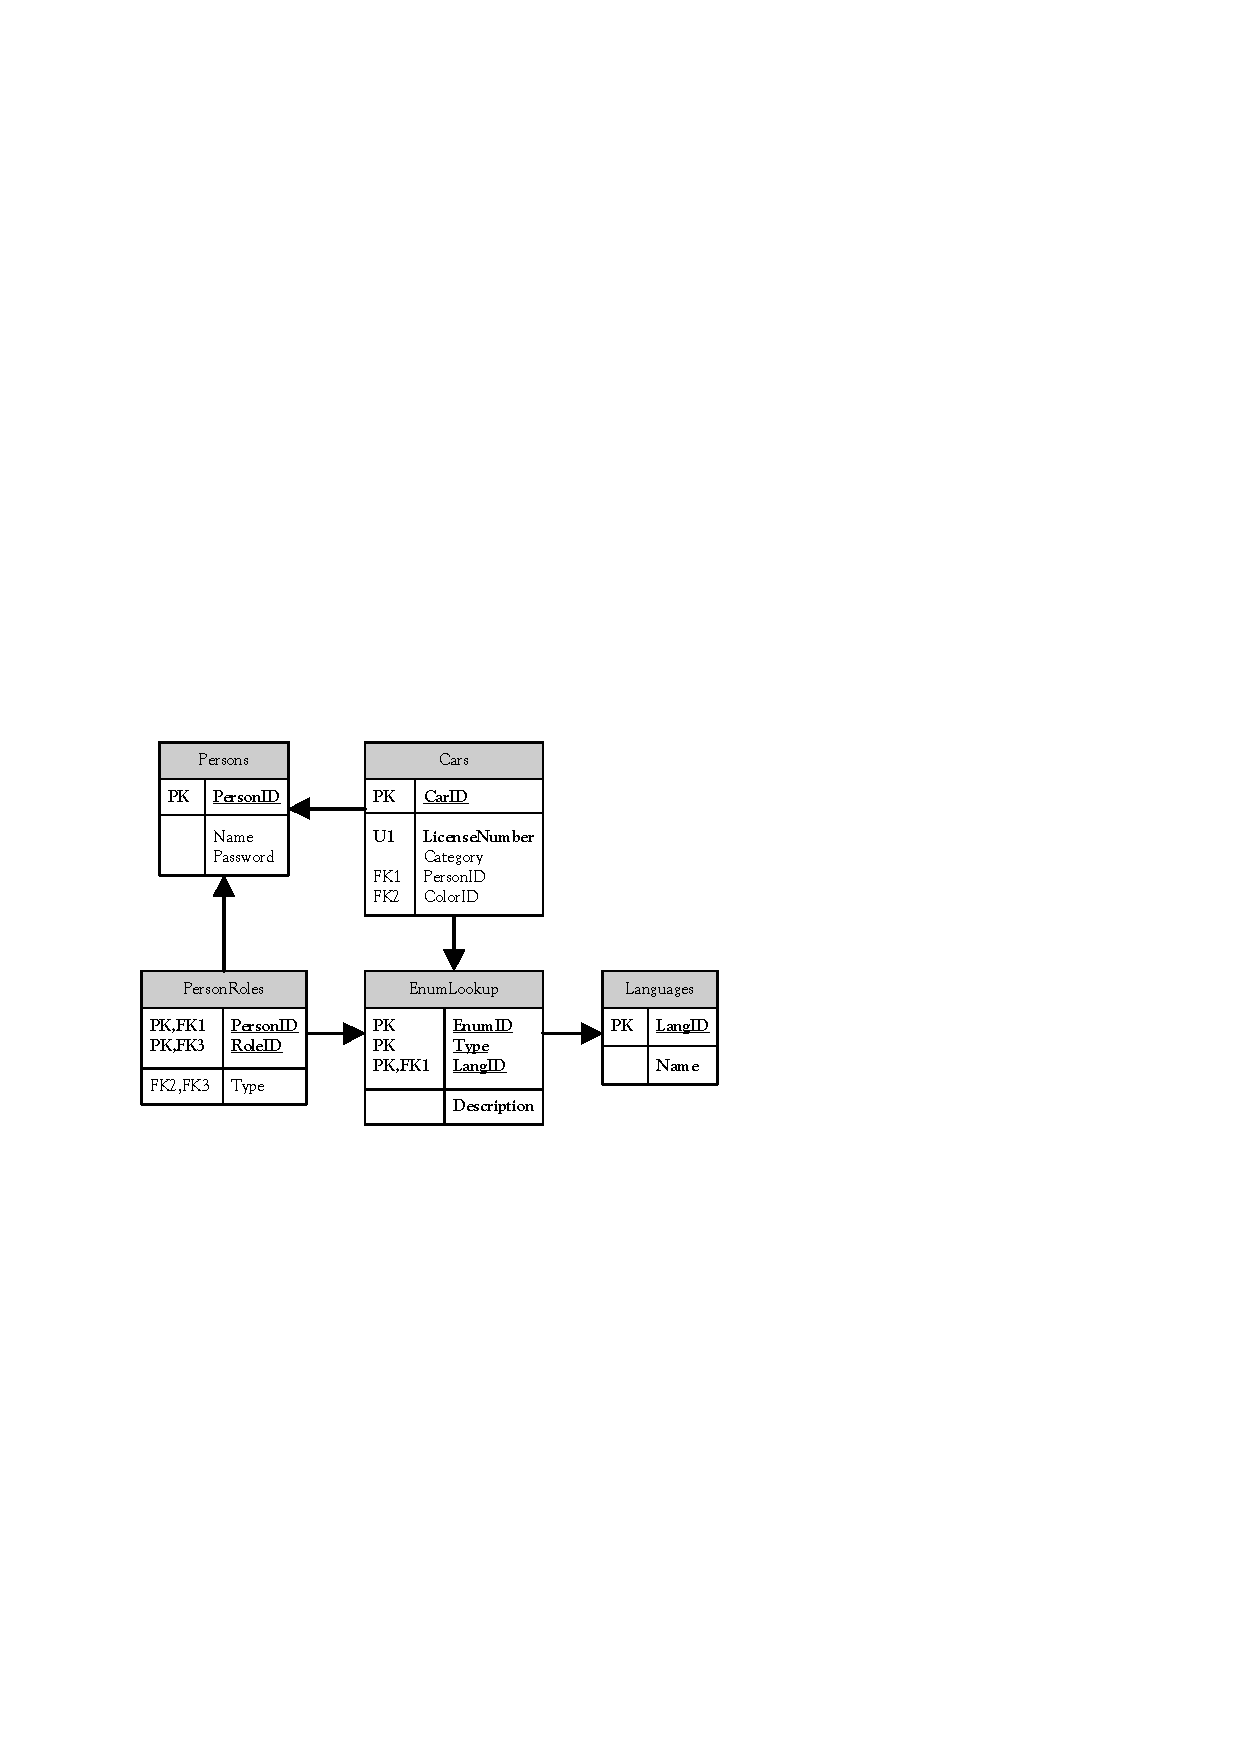
\includegraphics{./files/inc/figures/AnalysisEnumExtended}
				\caption{\label{fig:AnalysisEnumExtended} lookup table}
			\end{center}
		\end{figure}
		
		If descriptions of different tables are saved in one lookup table, you will 
		need to know which descriptions belong to which table. There are two 
		possibilities. You could define ranges of the ID belonging to a table. But 
		the better solution is to add a description type to the lookup table as you 
		can see in Figure \ref{fig:AnalysisEnumExtended}. That is one of the rare cases 
		where you could use an enum in the database if provided, because this values 
		will only be used in the code. The user will never see it.
		
		%-----
		\section{Loading lookup table data}
		
		There are several strategies to load data from lookup tables. Due to the fact this 
		data often are nearly static, it could be a good deal to read the data once 
		and hold in memory. 
		
		Another possibility is to get the values within one request. In Listing \ref{lst:enumJoinTables}
		you see an example of joining the tables. This statement can be used directly or by 
		creating a view on the database.
		
		\begin{lstlisting}[float=hbt,language={SQL},caption=join tables,label=lst:enumJoinTables]
SELECT c.LicenseNumber, p.Name, e.Description AS Color
FROM Cars AS c
	LEFT OUTER JOIN Persons AS p
		ON c.PersonID = p.PersonID
	LEFT OUTER JOIN EnumLookup AS e
		ON c.ColorID = e.EnumID
			AND EnumLookup.Type = 'cars'
			AND EnumLookup.LangID = 1
WHERE c.Category = 1
		\end{lstlisting}
\selectlanguage{ngerman}
%----------
\chapter{Makefiles}

	Es ist nicht m�glich, eine mit \textit{STORM} geschriebene Applikation mit Visual Studio
	in einem Schritt zu erstellen. Das Problem liegt beim CustomTool von CodeSmith. Zuerst
	wird aus den abstrakten Klassen eine DLL gebildet. Diese wird von CodeSmith verwendet
	um den Code zu generieren. Danach sollte die DLL mit dem neu dazugekommenen Code neu
	erzeugt werden. Dies ist jedoch erst nach einem Neustart von Visual Studio m�glich, 
	da die DLL durch das CodeSmith CustomTool blockiert wird.
	
	\section{L�sungsansatz}
	
		Mit Makefiles hat man die M�glichkeit die Applikation oder Libraries in einem Schritt 
		ohne das Aufstarten einer IDE zu erstellen. �nderungen in ben�tigten Dateien und 
		Abh�ngigkeiten werden automatisch erkannt.
		
		Wir haben zwei unabh�ngige Makefiles erstellt. Das eine �bernimmt das Bilden der 
		\textit{STORM} DLL. Damit ist es ebenfalls m�glich die DLL zu signieren und im GAC zu 
		registrieren.
		
		Mit dem zweiten Makefile ist es m�glich ein Assembly aus den abstrakten Klassen zu bilden, 
		daraus den ben�tigten Code zu generieren und dann die ganze HsrOrderApp Applikation zu 
		kompilieren. Das ganze geschieht mit einem einzigen Befehl.
		
	\section{Storm DLL}

		Das Makefile f�r die \textit{STORM} Library kann wie folgt ausgef�hrt werden:		
		\begin{Verbatim}
nmake [clean] [keys] [build] [install] [uninstall]
		\end{Verbatim}

		\begin{tabbing}
		  uninstall: \= \kill
			clean:     \> L�scht alle generierten Dateien aus dem Verzeichnis.\\
			keys:      \> Generiert ein Keypair.\\
			build:     \> Kompiliert und signiert den Code.\\
			install:   \> Registriert das Assembly im GAC.\\
			uninstall: \> Entfernt das Assembly aus dem GAC.\\
		\end{tabbing}

		In der Abbildung \ref{fig:analysisMakefilesStorm} sind die Abh�ngigkeiten der verschiedenen
		Schritte aufgezeigt. Wird zum Beispiel der Befehl \verb~install~ ausgef�hrt, wird auch �berpr�ft
		ob das Keypair vorliegt und die Storm.dll mit den aktuellsten Source Dateien kompiliert wurde.
		
		\begin{figure}[htb]
			\begin{center}
				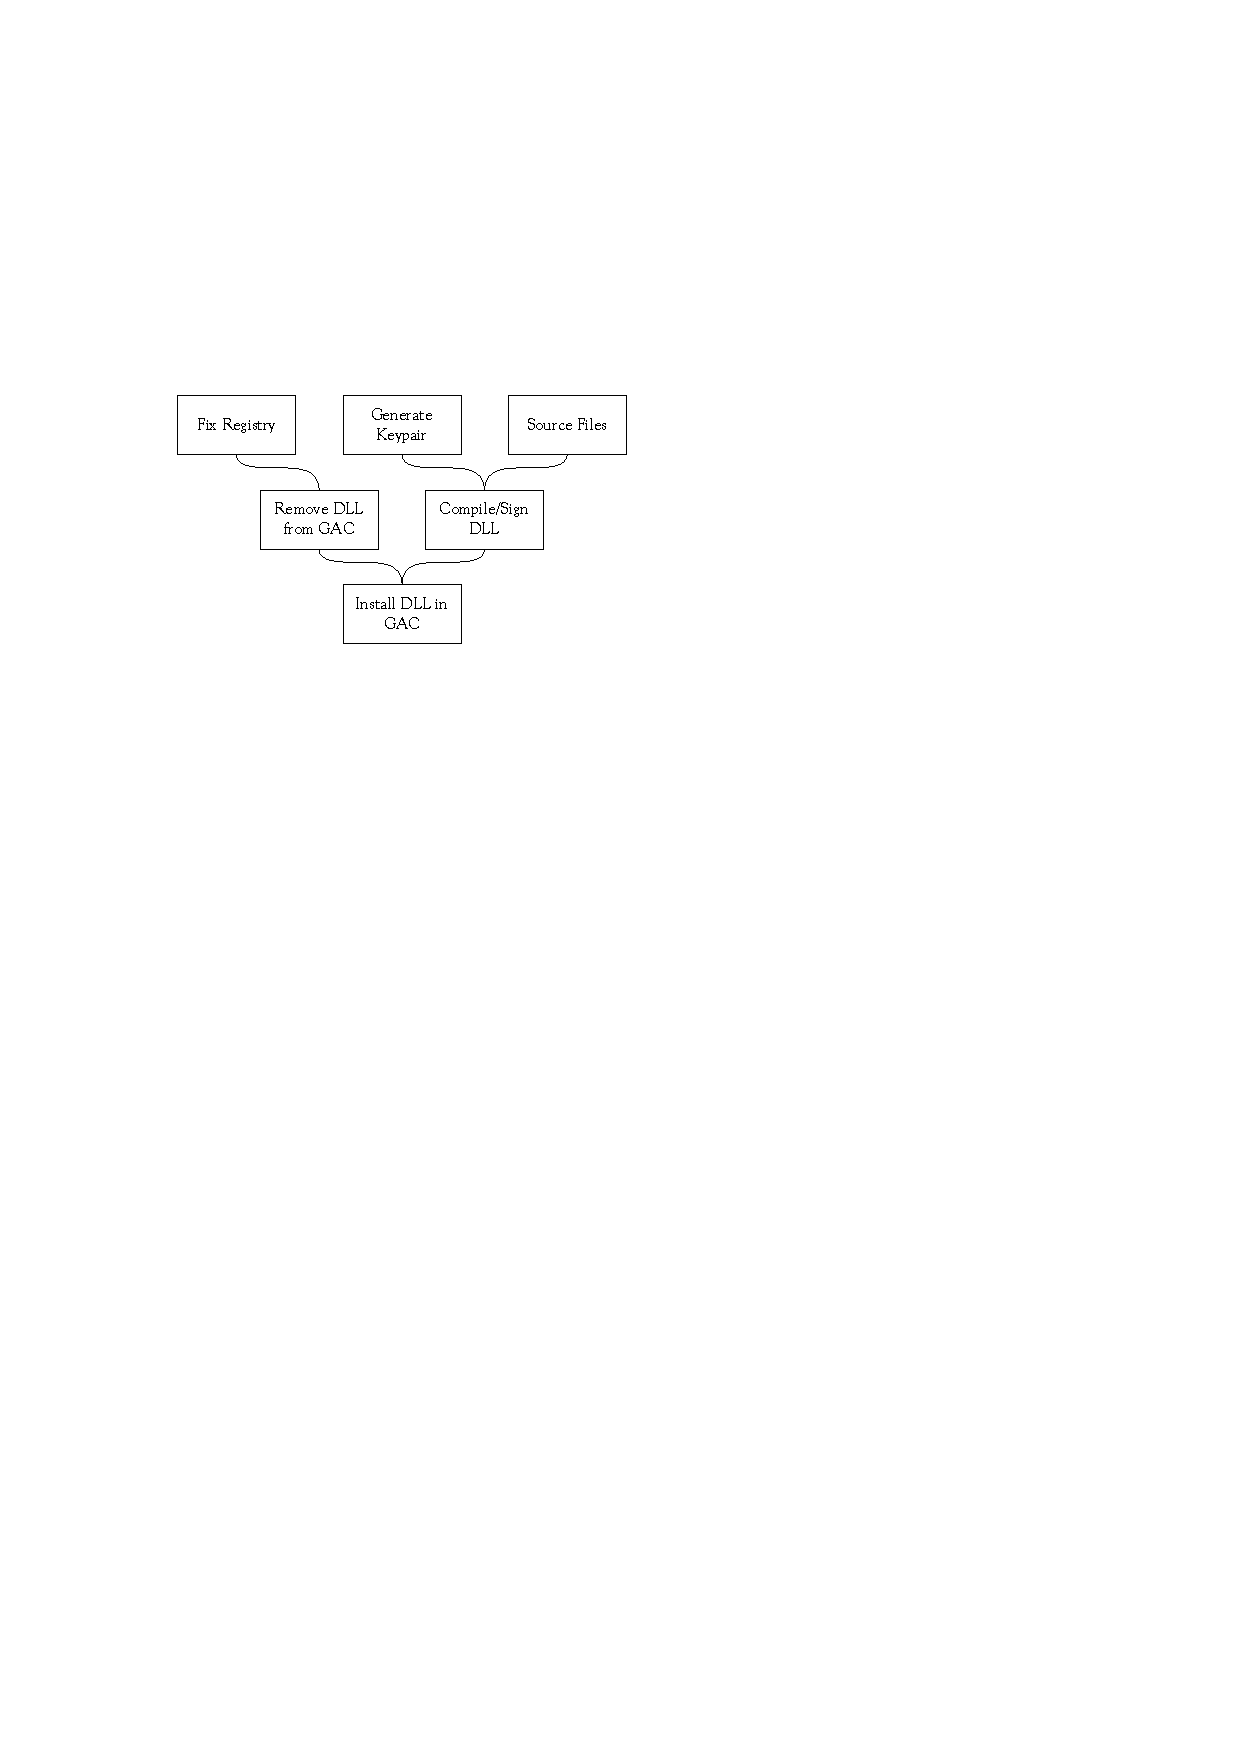
\includegraphics{./files/inc/figures/analysisMakefilesStorm}
				\caption{\label{fig:analysisMakefilesStorm} Storm Makefile}
			\end{center}
		\end{figure}

		Auf einigen Windows Installationen gibt es einen fehlerhaften Registry Eintrag, der wahrscheinlich 
		von einem Windows-Update stammt. Dieser verhindert, dass Assemblies aus dem GAC entfernt werden 
		k�nnen. Das Makefile l�scht diesen fehlerhaften Eintrag, bevor es versucht die DLL aus dem GAC zu 
		entfernen. Der Eintrag ist der Folgende:
		\begin{Verbatim}
[HKEY_LOCAL_MACHINE\SOFTWARE\Classes\Installer\Assemblies\Global]
@="..."
		\end{Verbatim}

\section{HsrOrderApp}
		
		Das Makefile f�r die HsrOrderApp kann wie folgt ausgef�hrt werden:		
		\begin{Verbatim}
nmake [clean] [impl] [mapper] [testapp] [run]
		\end{Verbatim}
		
		\begin{tabbing}
			testapp: \= \kill
			clean:   \> L�scht alle generierten Dateien aus dem Verzeichnis.\\
			impl:    \> Generiert mit Hilfe von CodeSmith die Implementations-Klassen\\
			         \> der Business-Objekte.\\
			mapper:  \> Generiert mit Hilfe von CodeSmith die Mapper-Klassen.\\
			testapp: \> Kompiliert die Applikation.\\
			run:     \> F�hrt die Applikation aus.\\
		\end{tabbing}
		
		Die Abbildung \ref{fig:analysisMakefilesOrderApp} zeigt die Abh�ngigkeiten beim bilden der 
		HsrOrderApp. Die Generierung von Domain Object Implementierungen und Mapper Klassen wurde 
		aufgeteilt, damit bei einer �nderung der Templates nur die betroffenen Dateien neu generiert 
		werden m�ssen. In der Abbildung wurde auf diese Aufteilung verzichtet.
		
		\begin{figure}[htb]
			\begin{center}
				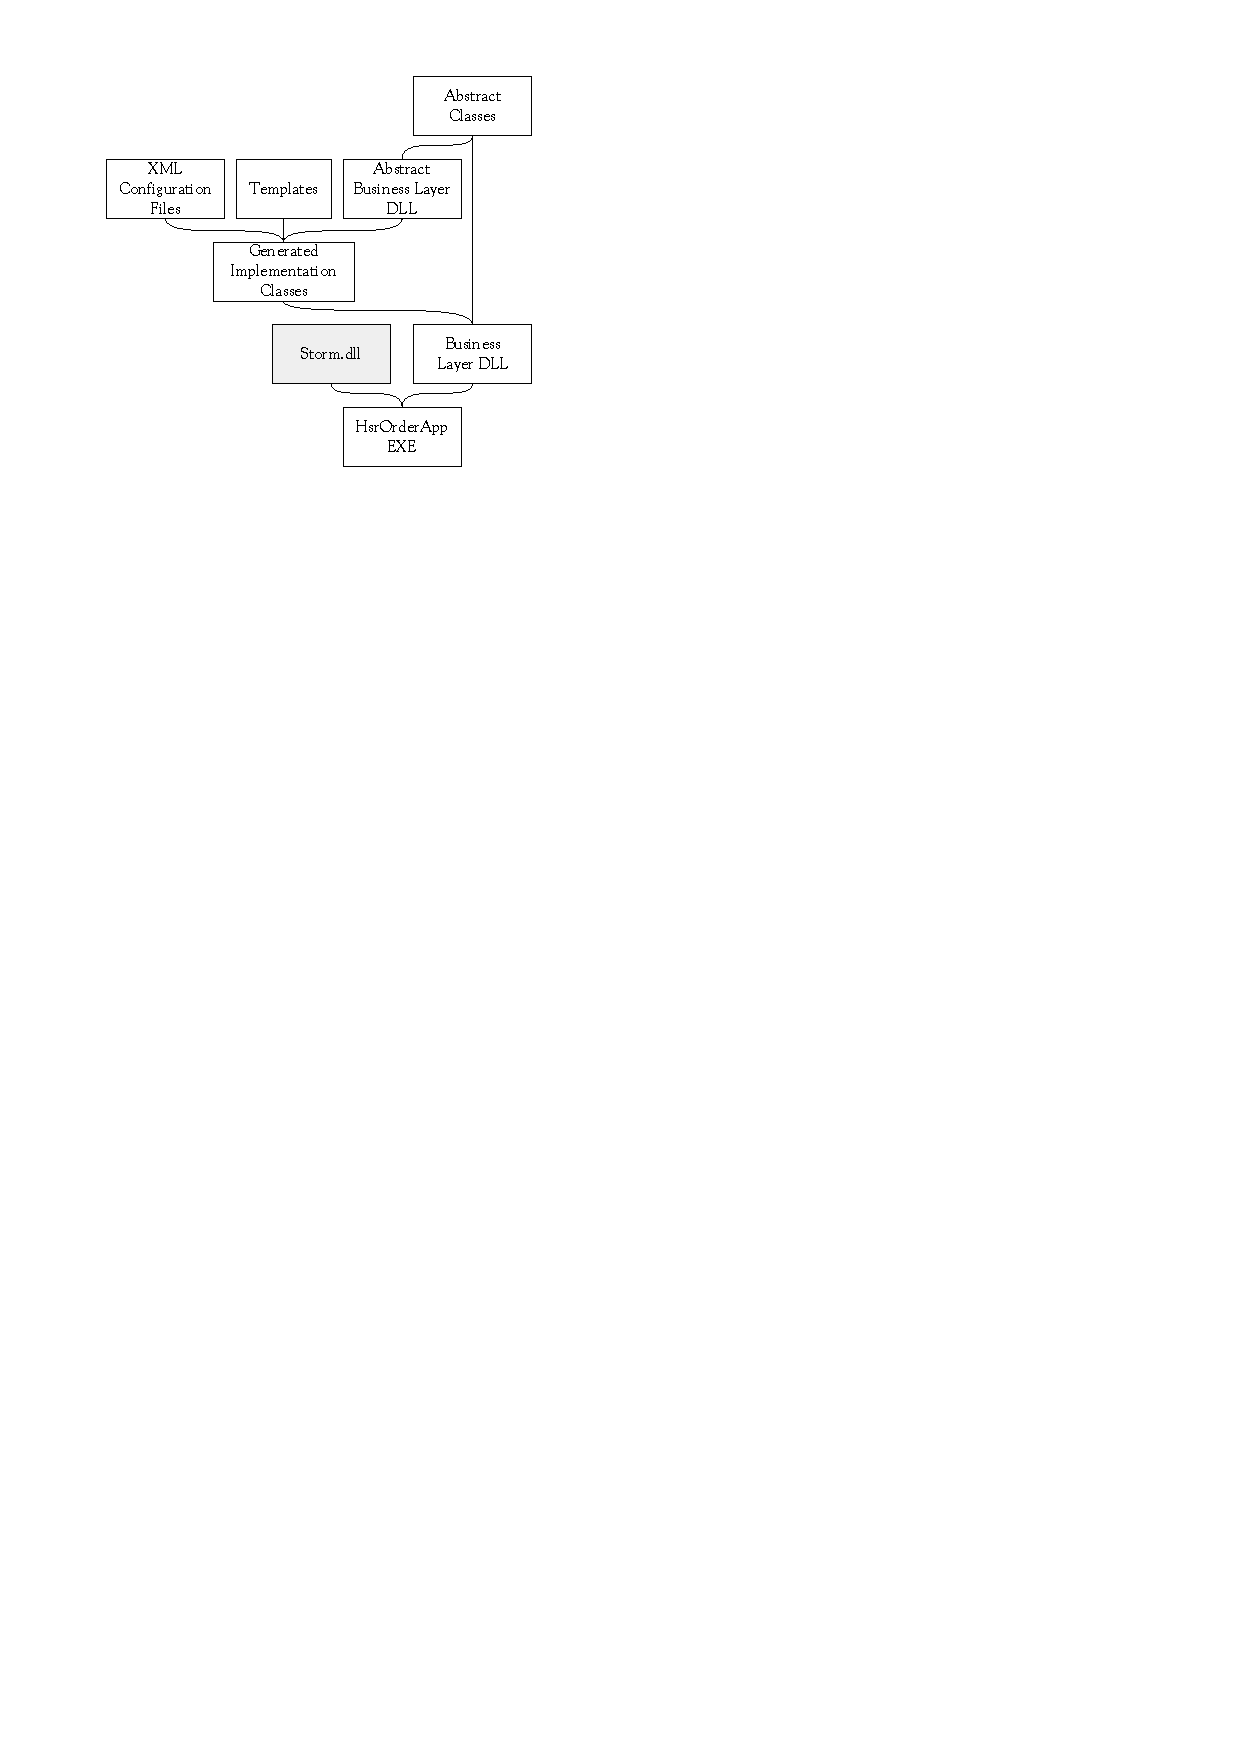
\includegraphics{./files/inc/figures/analysisMakefilesOrderApp}
				\caption{\label{fig:analysisMakefilesOrderApp} HsrOrderApp Makefile}
			\end{center}
		\end{figure}

		Die Datei Storm.dll wird vorausgesetzt und wird nicht automatisch erstellt.

	\section{Erkenntnisse}
		Den Build Prozess mit Makefiles zu automatisieren w�re eine sch�ne L�sung, den Code 
		auch ohne Visual Studio zu kompilieren. Ausserdem k�nnen andere Aufgaben wie Code 
		Generierung, Keypair erstellen, Code signieren und DLL im GAC registrieren im Build 
		Prozess eingebunden werden.
		
		Hier hat uns jedoch CodeSmith einen Strich durch die Rechnung gemacht. Denn aus 
		unerkl�rlichen Gr�nden, wird die DLL im GAC, w�hrend der Code Generierung, nicht 
		gefunden. Wir sind daher gezwungen unsere DLL ins Programm Verzeichnis von CodeSmith 
		zu kopieren, was alles andere als sch�n ist.


%\selectlanguage{english}
%\part{Technical Report}
%\label{par:technicalReport}

%\chapter{Overview}

	\section{About this document}
		This document has been written during a diploma thesis. It is the main
		part of the whole documentation and describes the core of this work. It gives
		a project overview and discusses all technical aspects.

	\section{Introduction}
		During 2003, three different versions of an order application were developed.
		This applications represent different approaches to deal with 
		databases. The application itself is not very complicated. It manages
		persons including addresses who can make orders. The respective database and
		application designs are discussed later in this document.
		
		The purpose of this work originated from the third of those applications. That version
		manages database related tasks through an O/R Mapper. Implementing such a mapper
		can be very challenging and error-prone. This is where \textit{STORM} comes into play.
		The idea behind it is to have a framework which generates all mapping code automatically,
		based on input parameters. This document describes how this can be achieved and also
		explains the limitation of such an approach. As a reference implementation to prove
		the usability of \textit{STORM}, a fourth order application has been created.
		Throughout this document, all implementation examples are taken from this reference
		implementation. At chapter \ref{cha:createApplication} the reference application 
		is taken as a real world example to show how to develop an application with \textit{STORM}.
		
		
	\section{About O/R Mapping}
		Today, most new applications are developed by using an object oriented programming
		language like C++ or C\#. Nevertheless, most databases have a relational structure.
		Relational means that relations between objects are always be modelled by defining foreign
		keys in tables. This structural difference is known as ``type mismatch''. Because of that, a mechanism
		is needed that provides a way to work with databases in an easy as possible way. One
		possibility is to use datasets. Datasets have a similar structure to that of a relational 
		database and are built-in types in C\#.
		This method was implemented in the first version of the order application.
		Another possibility is to write code which manages all the mapping. Namely this means
		mapping classes to tables, variables to columns, etc. This has the advantage that
		a programmer can code in a pure object oriented manner an does need to pay less
		attention to the database. For him, database tasks are done automatically. Although most
		O/R mapper, including \textit{STORM}, have more features implemented, mapping the in-memory
		structure to the database structure is the most important task of an O/R mapper.
	
	%---------
	\section{How to start}
		At the end, an O/R mapper is nothing else than code that is responsible for
		certain tasks. There are several methods to create this code. A catchphrase in 
		the context of software engineering is ``generic programming''. Generic programming is 
		a technique aiming at writing programs as general as possible, 
		without sacrificing efficiency by doing overgeneralising. Another technique is called
		``generative programming''. Generative programming enables programs to be automatically
		constructed. There are more programming techniques like aspect-oriented or functional
		programming which are not taken into account here.
		
		Both, generic and generative programming have their strengths and weaknesses.
		The third order application made use of the generic programming technique. As
		a counterpart, this thesis should result in the knowledge of the usability
		of a generative programming technique for this specific problem.
		
		As stated before, a generative programming technique enables programs to be automatically
		constructed. This sounds promising, but before one can start writing a program
		which constructs another program, he needs to define a starting point. Transferred
		to the problem of O/R mapping, this means that one needs to define where to make
		the mapping definitions. Three scenarios would be sensible:
		\begin{itemize}
			\item The database design is the starting point. Out of this design, all domain objects
						and the mapping code are generated.
			\item The domain model is the starting point. Out of this, the database tables and the mapping
						code are generated.
			\item Both, the domain model and the database design are taken as starting point. Additionally, the mapping 
						needs to be defined. Out of this, the mapping code is generated.
		\end{itemize} 
		
		Which approach should be chosen depends on the requirements for a given project. Each
		has been realised in commercial and open source projects. In this thesis,
		we have chosen to use the second approach where the domain model should be taken as starting point.
		Although with this approach the database tables could be generated automatically, it is not
		implemented because we use the existing database from the previous order applications. This is
		not a problem, because the mapping can be specified in the domain objects and this works
		whether the database tables are generated or already exist. 
				
	
%\chapter{Requirements Overview}

	\section{\textit{STORM} external}
		The main advantage of using a tool like \textit{STORM} is the time savings in
		project developments and the accuracy of the generated code. This in mind, the
		following requirements are specified:
		
		\begin{itemize}
			\item Mapping between the in-memory objects and the database tables is done automatically.
			\item Easy and understandable configuration and usage.
			\item There are no other dependencies than to CodeSmith, such that \textit{STORM} can
						be used independently.
			\item Is integrated in the make process of the Visual Studio .NET.
			\item Can also be used without Visual Studio .NET.
			\item The resulting program is efficient regarding network performance.
		\end{itemize}
		
		This is one would expect from this framework.
		Because it is not always easy to write templates for a general purpose,
		it is important to keep the target in mind. A framework like \textit{STORM}
		cannot cover all requirements which can occur in any project. An exactly
		defined boundary is needed. This boundary defines which problems can be solved
		with \textit{STORM}. It is described in the next section and in more
		detail in later chapters. The above requirements are of general nature and
		apply to every project which uses the technique of generative programming in
		the scope of an O/R Mapper.
	
	\section{\textit{STORM} internal}
		These requirements are more specific and could be called ``features of
		\textit{STORM}''. They are not directly connected with the usage of the 
		framework but affect the design of it. This list of features could
		be extended in many ways but it is a good starting point:
		
		\begin{itemize}
			\item No dependencies between the framework, the generated code and the code which
						uses them (namely a client) may exist.
			\item A locking mechanism is implemented.
			\item Insert, update and delete statements are handled by the framework and
						executed in the right order.
			\item SQL code is hidden from the user and generated automatically.
			\item Custom finder methods can be defined.
			\item Custom constructors can be defined.
			\item Transferred objects are stored to minimize remote calls.
			\item Data integrity is ensured.
			\item A well defined set of database mapping types are supported.
		\end{itemize}
		
		Most of these requirements are not easy to implement but even though, they are very
		important in terms of the usability of the framework. These requirements are
		a starting point for the whole design. Every one will be discussed in detail
		in this document.
		
		Because most of the above requirements can be solved by using and applying 
		appropriate patterns, the next section is devoted to these patterns.
% \input{./files/techReportAnalysis}
%\chapter{Patterns Discussion}

	\section{Why Patterns}
		A pattern describes both a problem which occurs over and over again and
		the core of the solution to that problem. This solution can be used
		whenever this or a similar problem exists. Patterns can be combined and are 
		therefore a valuable design strategy for large applications. There are many advantages
		of using patterns over a classical design. The scope of this thesis is not to 
		list all of the advantages but to talk about specific patterns which are worth studying
		for this purpose.
		
		Not all of the following patterns describe a technically complex problem but they
		give a vocabulary to talk about problems in a manner which everybody understands
		easily who knows this vocabulary.
		
	\section{Which Patterns}
		There exists thousands of patterns out there. Not all patterns are relevant
		for a given application, in fact, a minority is. This raises the problem
		of choosing the patterns, which should be done carefully because it directly
		affects the application's design.

		The following list is a summary of all patterns relevant for this thesis. They are 
		mainly taken from M. Fowler \cite{Fowler03}. The list is in alphabetical order.
		\LTXtable{\linewidth}{./files/inc/tables/patternsUsedPatterns}

	\section{Describe the Patterns}
		Of course, one needs to know what a pattern at the end does and which
		benefits it provides. First, each pattern mentioned in the last section will 
		be described separately before they are put in a big context. The following 
		description is not meant as a complete reference but as a short description
		of each relevant pattern. Especially implementation details are left aside. They will be
		addressed in further chapters. Event though, this description should give enough information to understand
		what each pattern is for. For a more detailed discussion of these patterns, please read
		M. Fowler's Patterns of Enterprise Application Architecture \cite{Fowler03}.
		
		\subsection{Domain Model}
		\label{subsec:domainModel}
			The domain model pattern essentially describes that the domain layer
			is organised in an object-oriented (OO) manner. This technique is commonly
			used and understood and therefore not described in further detail. 
			
		\subsection{Service Layer}
		\label{subsec:serviceLayer}
			Enterprise applications often have different interfaces which provide access to
			business logic and data they store. Common interfaces are those for web-services,
			user interfaces, data loader, etc. A \textit{Service Layer} defines a boundary to
			the application and available operations (see Figure \ref{fig:patternsServiceLayer}). 
			Therefore, it encapsulates the application's business logic. To separate business 
			logic from the client interfaces has several advantages. First, the interface and therefore all
			possible operations are well defined and relatively easy to use for clients. Second,
			it reduces the burden of multiple implementations of the same functionality and improves code
			maintainability. A \textit{Remote Facade} (\ref{subsec:remoteFacade}) is an 
			example of a \textit{Service Layer}.
			
			\begin{figure}[htb]
				\begin{center}
					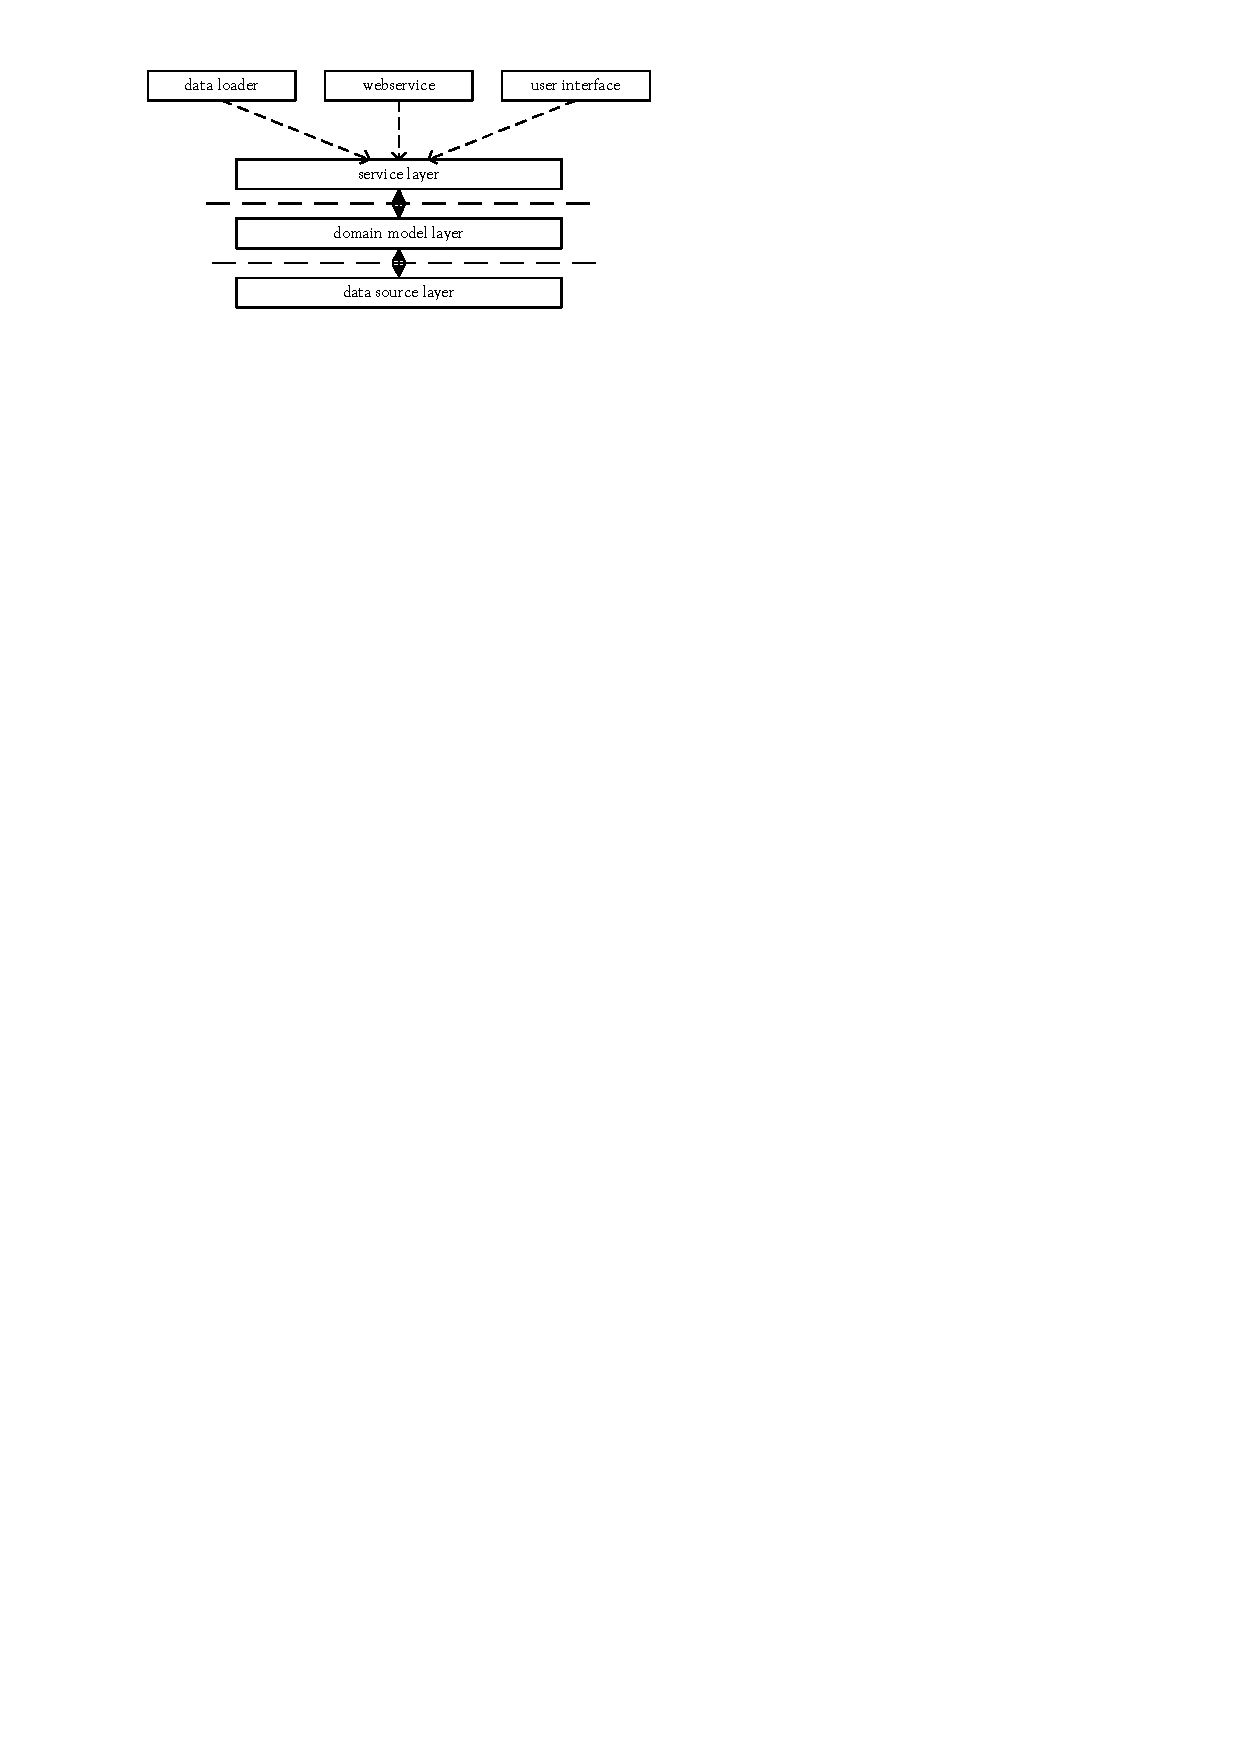
\includegraphics{./files/inc/figures/patternsServiceLayer}
					\caption{\label{fig:patternsServiceLayer} Service Layer defines application's boundary}
				\end{center}
			\end{figure}
	
		\subsection{Data Mapper}
		\label{subsec:dataMapper}
			A \textit{Data Mapper} is a layer between Domain Objects and a Database.
			A \textit{Data Mapper} is used because Objects and a relational database have
			different mechanisms for structuring data. The \textit{Data Mapper} separates in-memory objects 
			from the database and transfers data between the two. With this pattern,
			the in-memory objects do not need to know about the database at all. Figure
			\ref{fig:patternsDataMapperOverview} shows the general idea of a \textit{Data Mapper}.

			\begin{figure}[htb]
				\begin{center}
					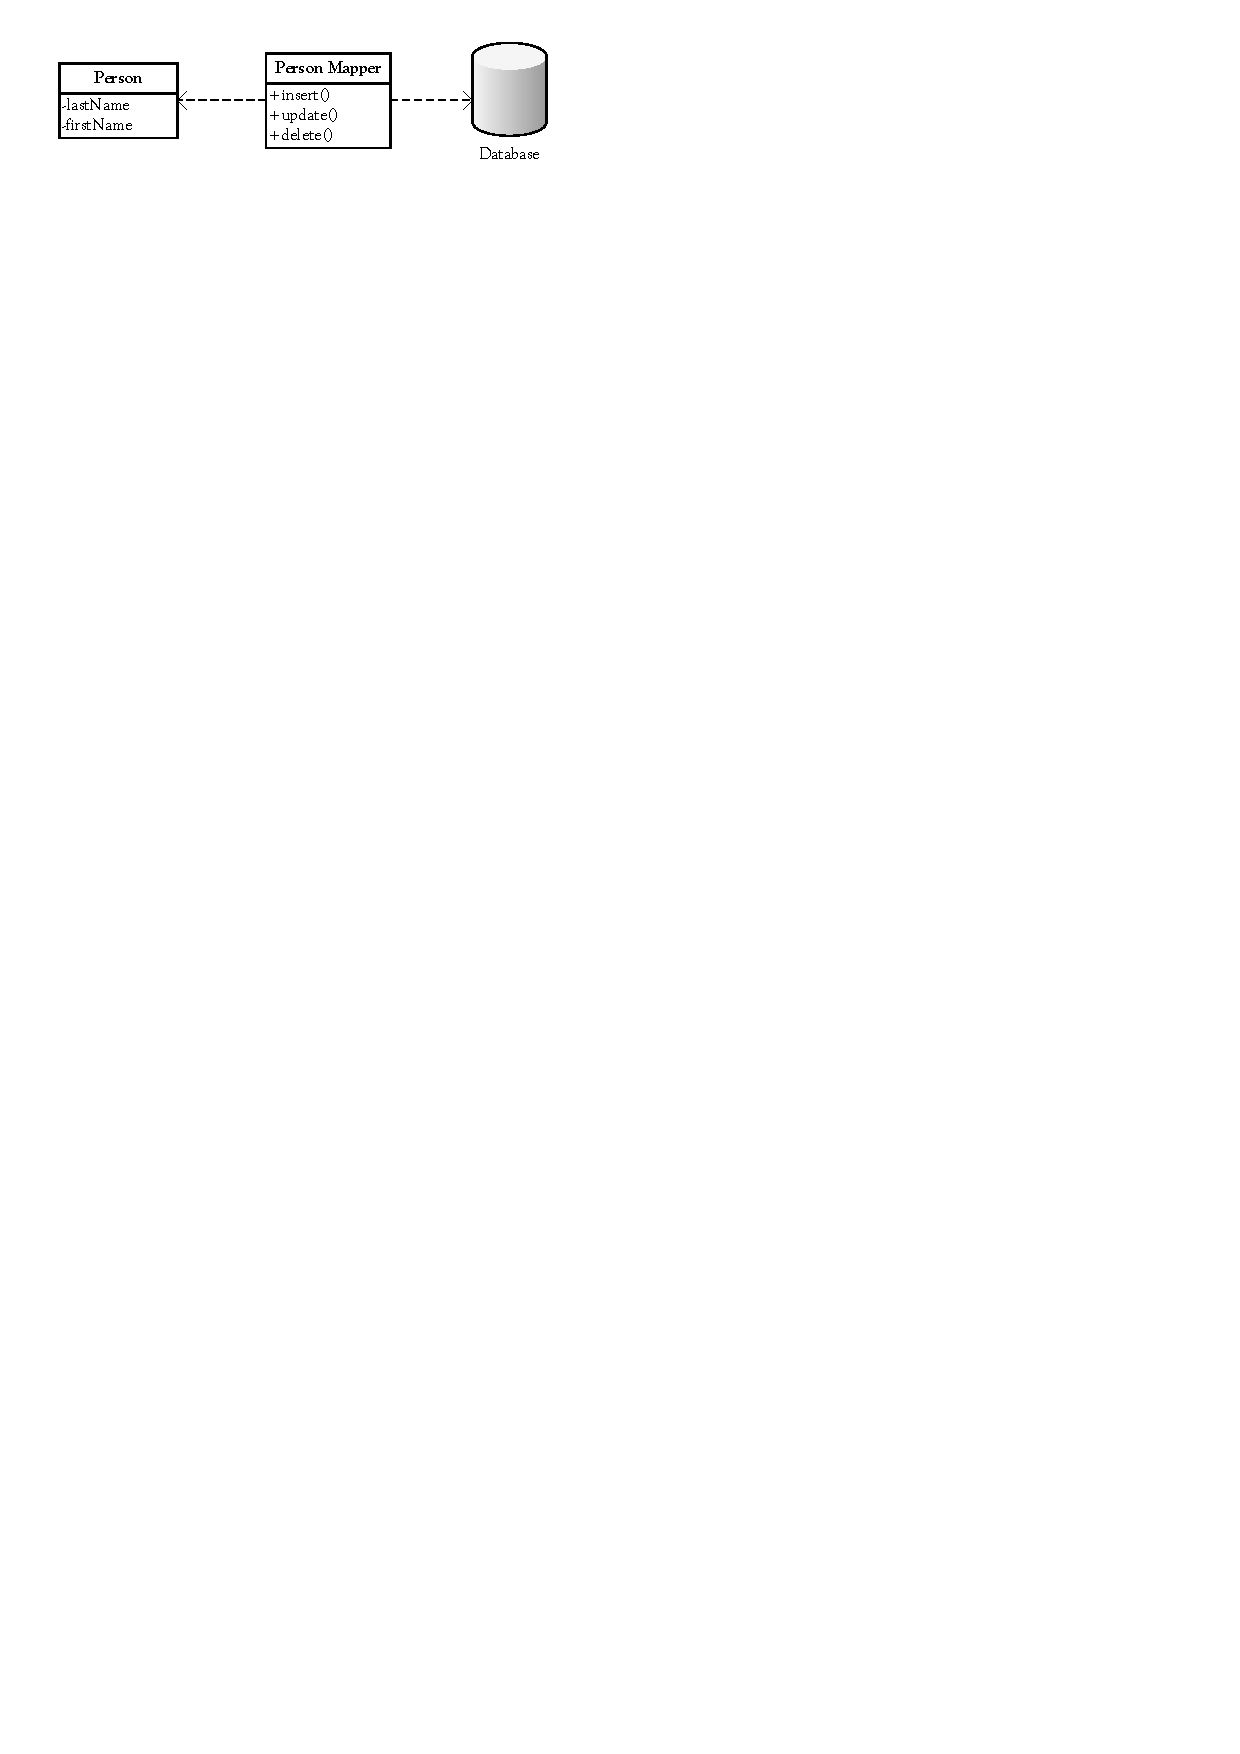
\includegraphics{./files/inc/figures/patternsDataMapperOverview}
					\caption{\label{fig:patternsDataMapperOverview} Data Mapper Overview}
				\end{center}
			\end{figure}
			The whole layer of \textit{Data Mapper} can be substituted, either for testing purposes
			or to allow a single domain layer to work with different kind of databases. This
			becomes very powerful if a \textit{Data Mapper} is combined with other patterns. This topic
			will be addressed in later chapters.
			
		\subsection{Identity Map}
		\label{subsec:identityMap}
			The basic idea behind \textit{Identity Map} is to have a series of maps containing objects
			that have been pulled from the database. If you load an object from the database,
			you first check the maps. If there already is an object which corresponds to the
			one you are loading, you do not need to load it. This is illustrated in Figure
			\ref{fig:patternsIdentityMap} 

			How many maps are needed depends on the application. You can either choose one
			map per class or one map for the whole session. 

			\begin{figure}[htb]
				\begin{center}
					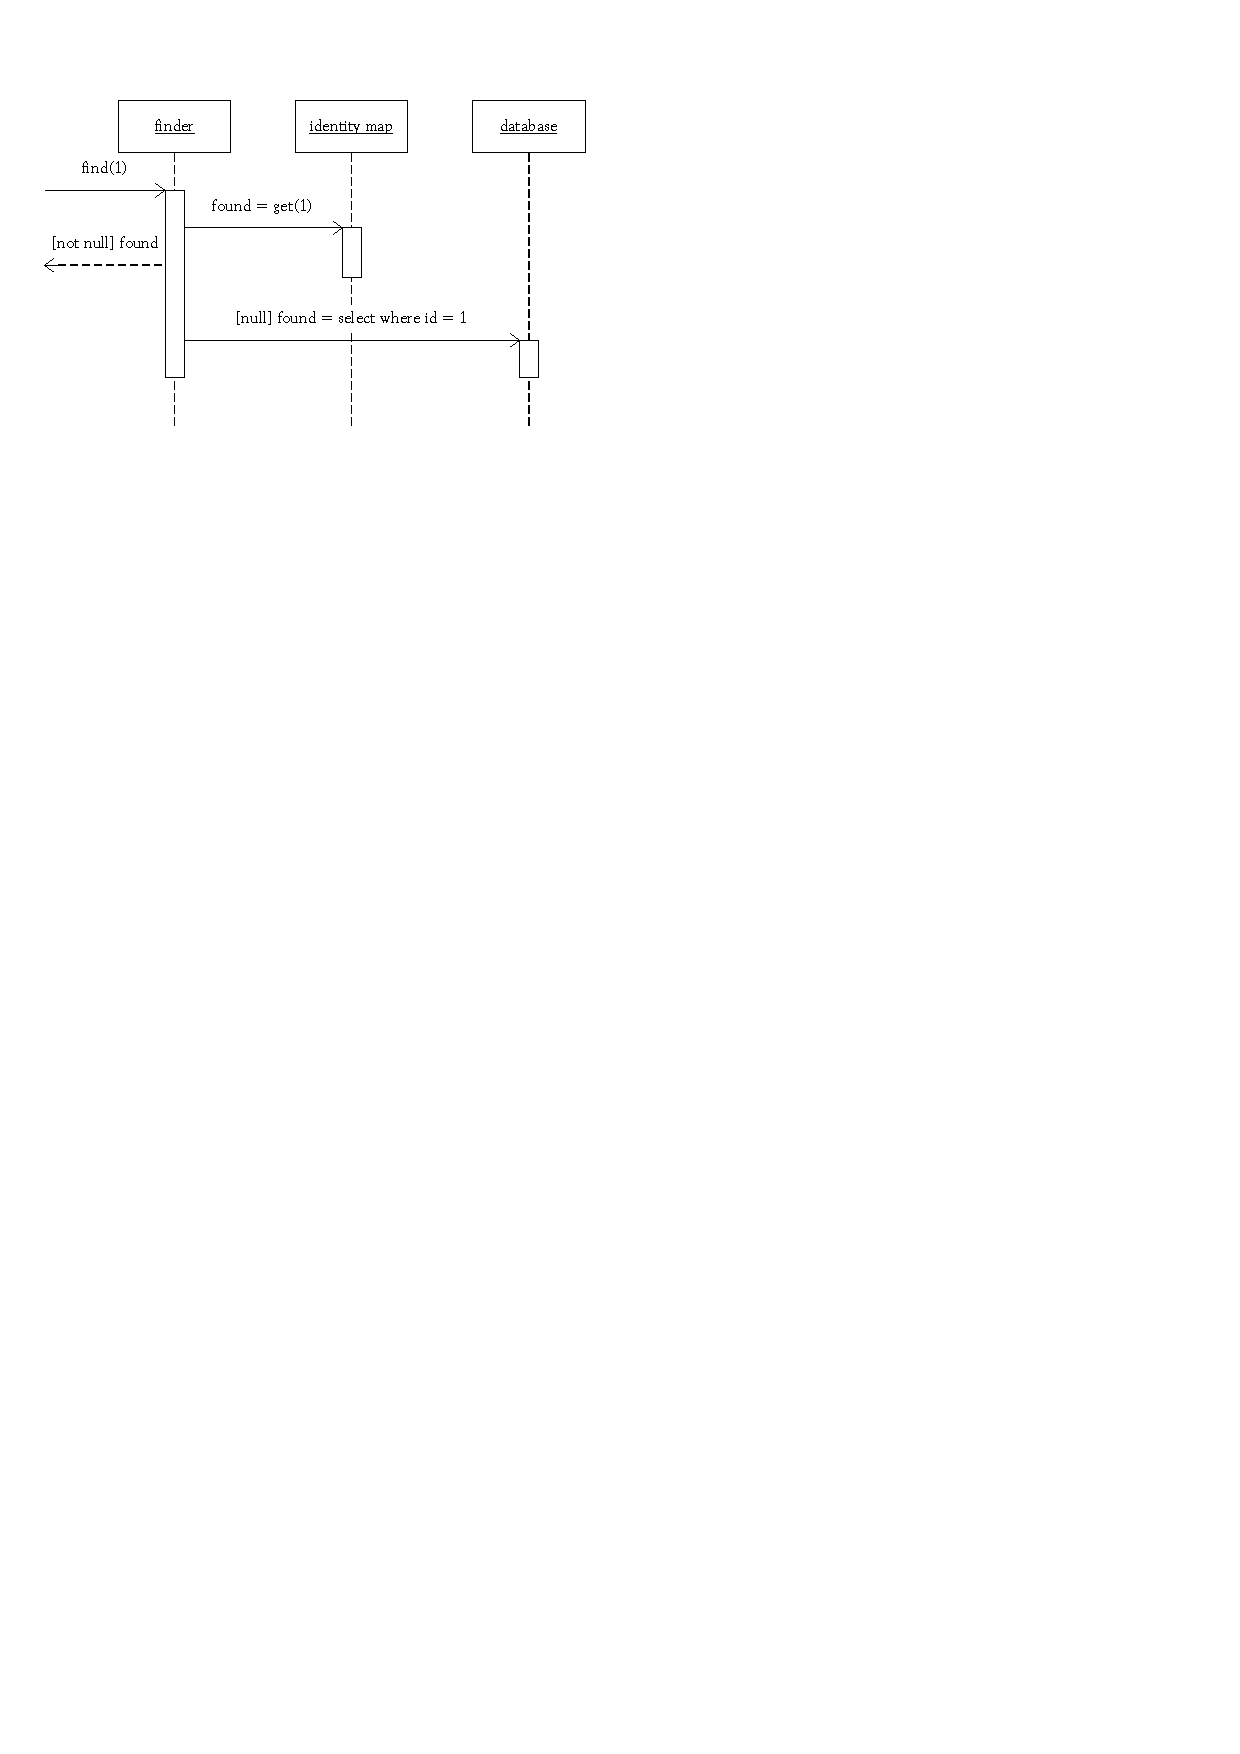
\includegraphics{./files/inc/figures/patternsIdentityMap}
					\caption{\label{fig:patternsIdentityMap} Mapping a collection to a foreign key}
				\end{center}
			\end{figure}

		\subsection{Lazy Load}
		\label{subsec:lazyLoad}
			If you load an object from the database into memory it is often useful to
			load objects that are related to it. This makes working with objects easier,
			because you don't have to load every single object yourself. The drawback of
			this mechanism is that it can have the effect of loading a huge number of
			related objects. This in turn can hurt the performance of your application
			drastically, especially when only a few objects are actually needed.
			\textit{Lazy Load} interrupts this loading process and leaves a marker in the
			object structure so that it can be loaded only 
			when it is used. This is shown in Figure \ref{fig:patternsLazyLoad1}.

			\begin{figure}[htb]
				\begin{center}
					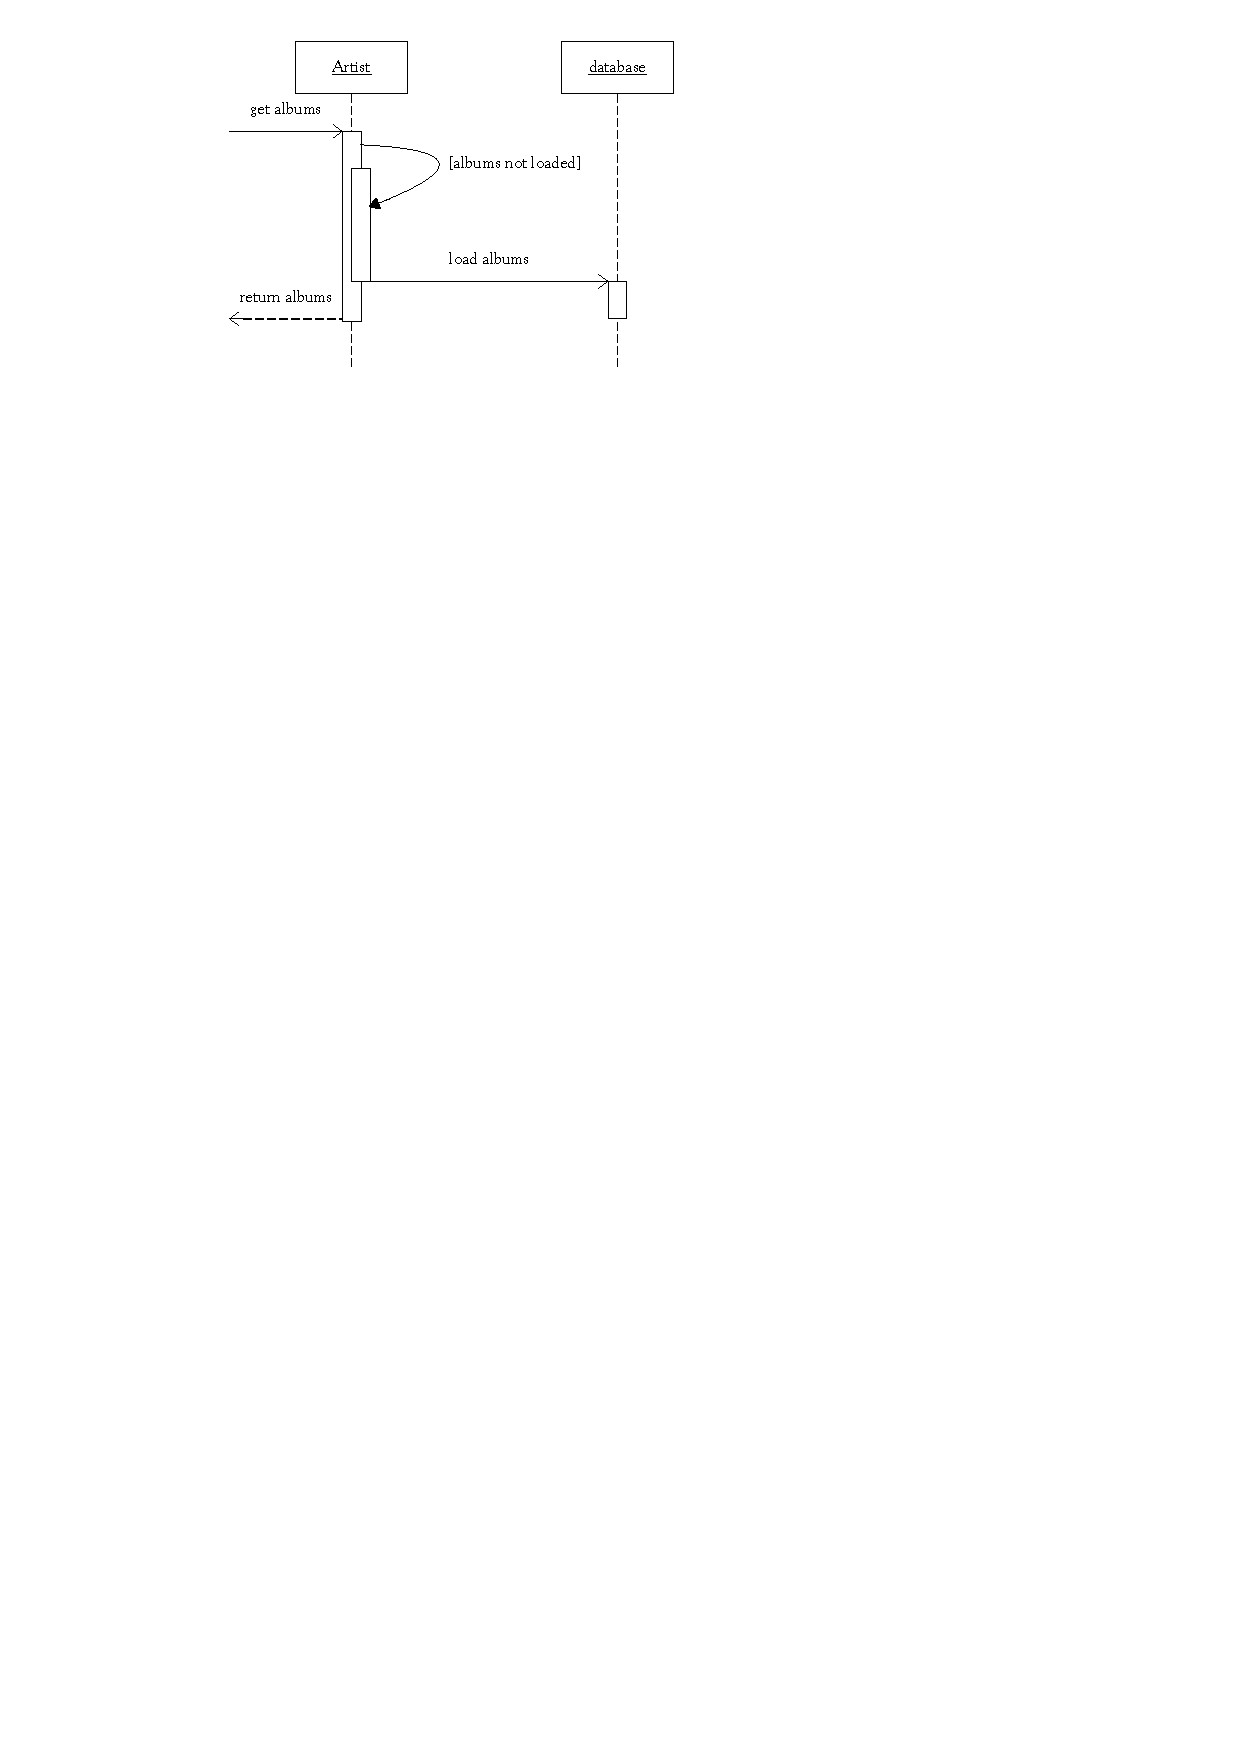
\includegraphics{./files/inc/figures/patternsLazyLoad1}
					\caption{\label{fig:patternsLazyLoad1} Sample Lazy Load Sequence}
				\end{center}
			\end{figure}
			Using \textit{Lazy Load} does not always improve performance. For instance, if
			you need to load all related objects, Lazy Load can even make performance
			worse that it was without it.

			There are four ways for implementing \textit{Lazy Load}
			\begin{itemize}
				\item Lazy Initialisation
				\item Virtual Proxy
				\item Value Holder
				\item Ghost
			\end{itemize}
			All of this methods have their own benefits and drawbacks but for the purpose of
			this thesis, a \textit{Virtual Proxy} pattern seems the most powerful and appropriate. A \textit{Virtual
			Proxy} is an object that looks like a real object but does not contain any data. Only when
			one of its methods is called does it load the correct object from the database. This pattern is
			described in E. Gamma's Design Patterns \cite{Gamma97}.
			
		\subsection{Unit of Work}
		\label{subsec:unitOfWork}
			It is important to know what you change in your domain model in order to apply those
			changes to the database. A \textit{Unit of Work} keeps track of what you have done
			during a business transaction and figures out what needs to be done to get the
			database in a consistent state. Therefore, a \textit{Unit of Word} needs to be informed
			every time an object is change, created or deleted. There are different ways to
			implement this. Either the user of an object register the object with the 
			\textit{Unit of Work} and mark objects as dirty after making any changes or
			the \textit{Unit of Work} handles this by its own. The latter case is preferable
			because it is less fault-prone. Figure \ref{fig:patternsUnitOfWork} shows the 
			working mechanism of this pattern.
		
			\begin{figure}[htb]
				\begin{center}
					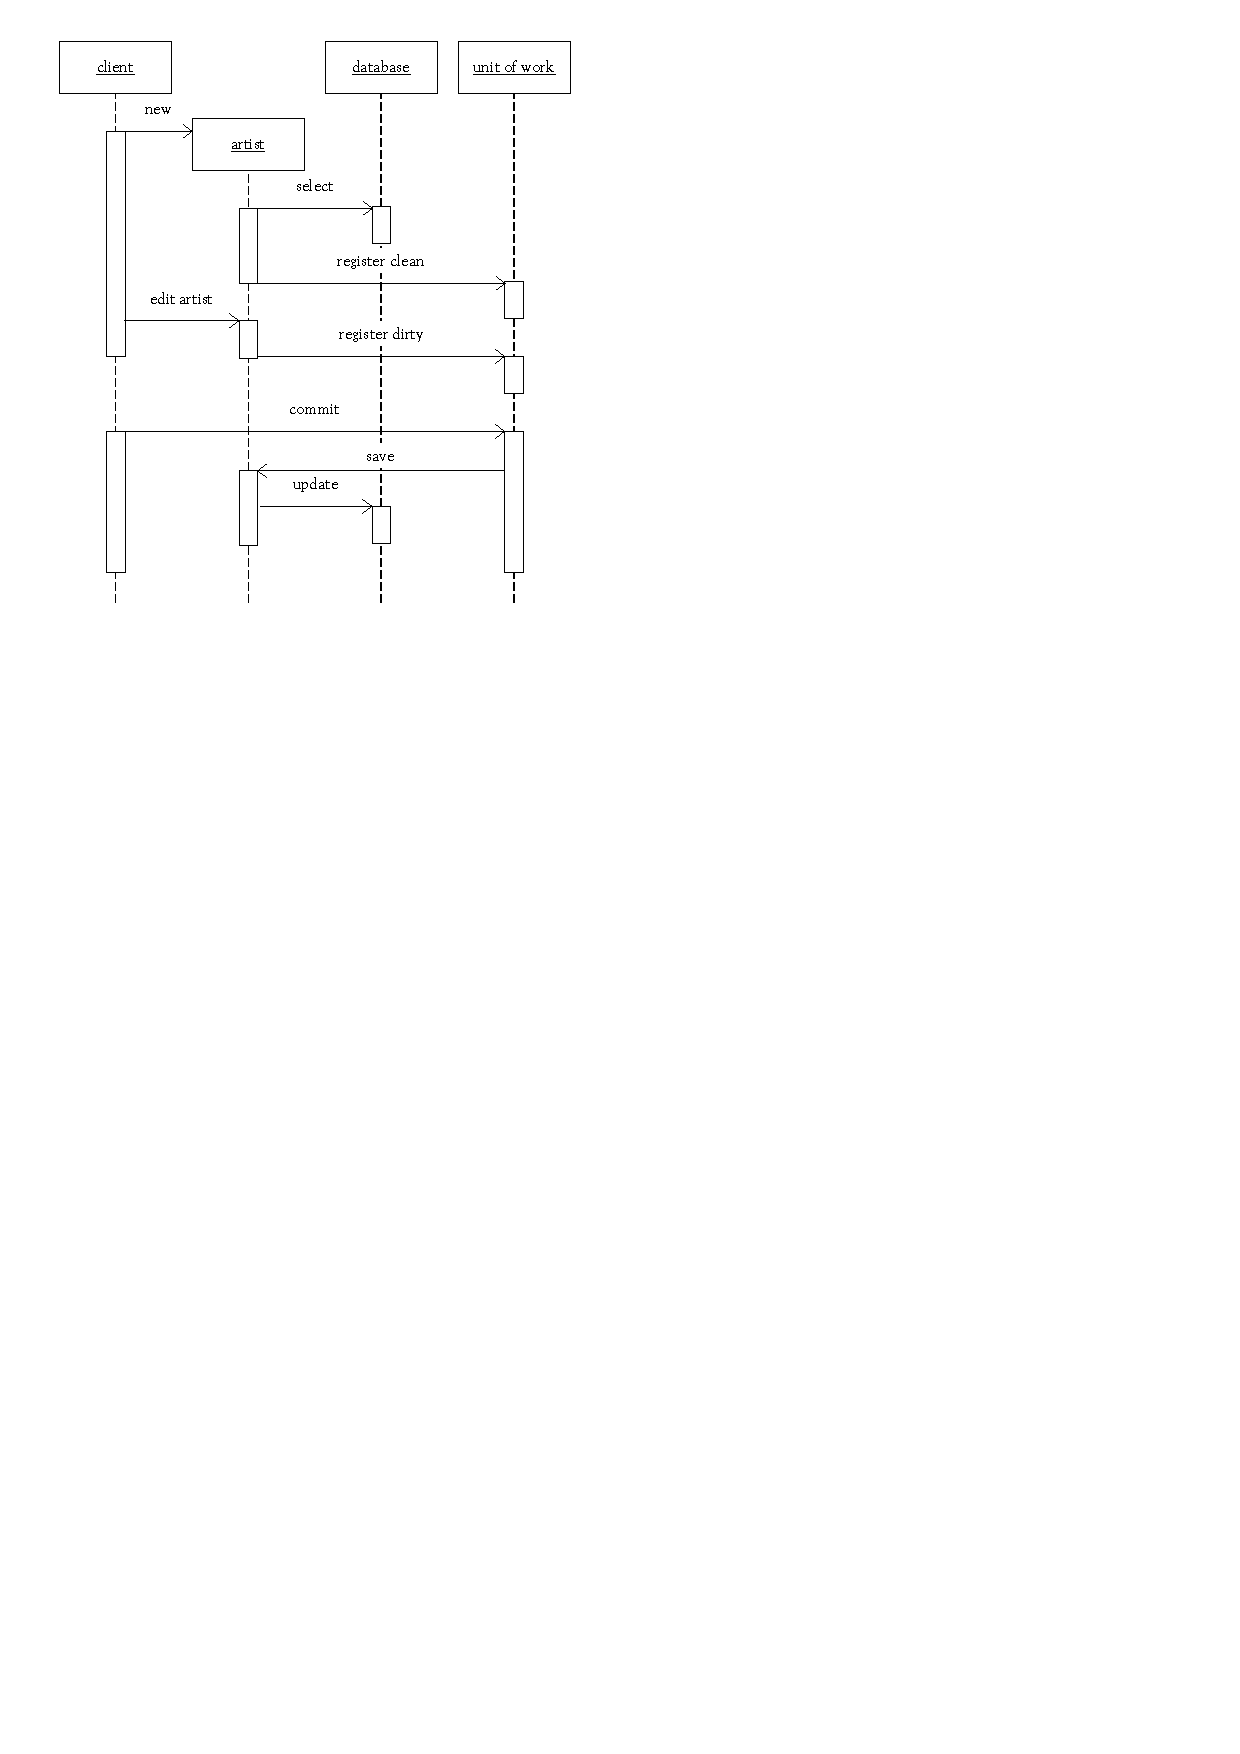
\includegraphics{./files/inc/figures/patternsUnitOfWork}
					\caption{\label{fig:patternsUnitOfWork} Unit of work mechanism}
				\end{center}
			\end{figure}
			
		\subsection{Foreign Key Mapping}
		\label{subsec:foreignKeyMapping}
			In an object-oriented system, objects are connected to each other directly or by object
			references. Relational databases use foreign key references for this. To save an object
			to a database, it is important to save these object references and map them to foreign 
			key references on the database. This is, what a \textit{Foreign Key Mapping} pattern does, it maps
			an object reference to a foreign key.

			These mappings can be of different kind and complexity. The simplest case is, if two
			objects are linked together. This association can be replaced
			by a foreign key in the database. This is shown in Figure \ref{fig:patternsForeignKeyMapping1}.

			\begin{figure}[htb]
				\begin{center}
					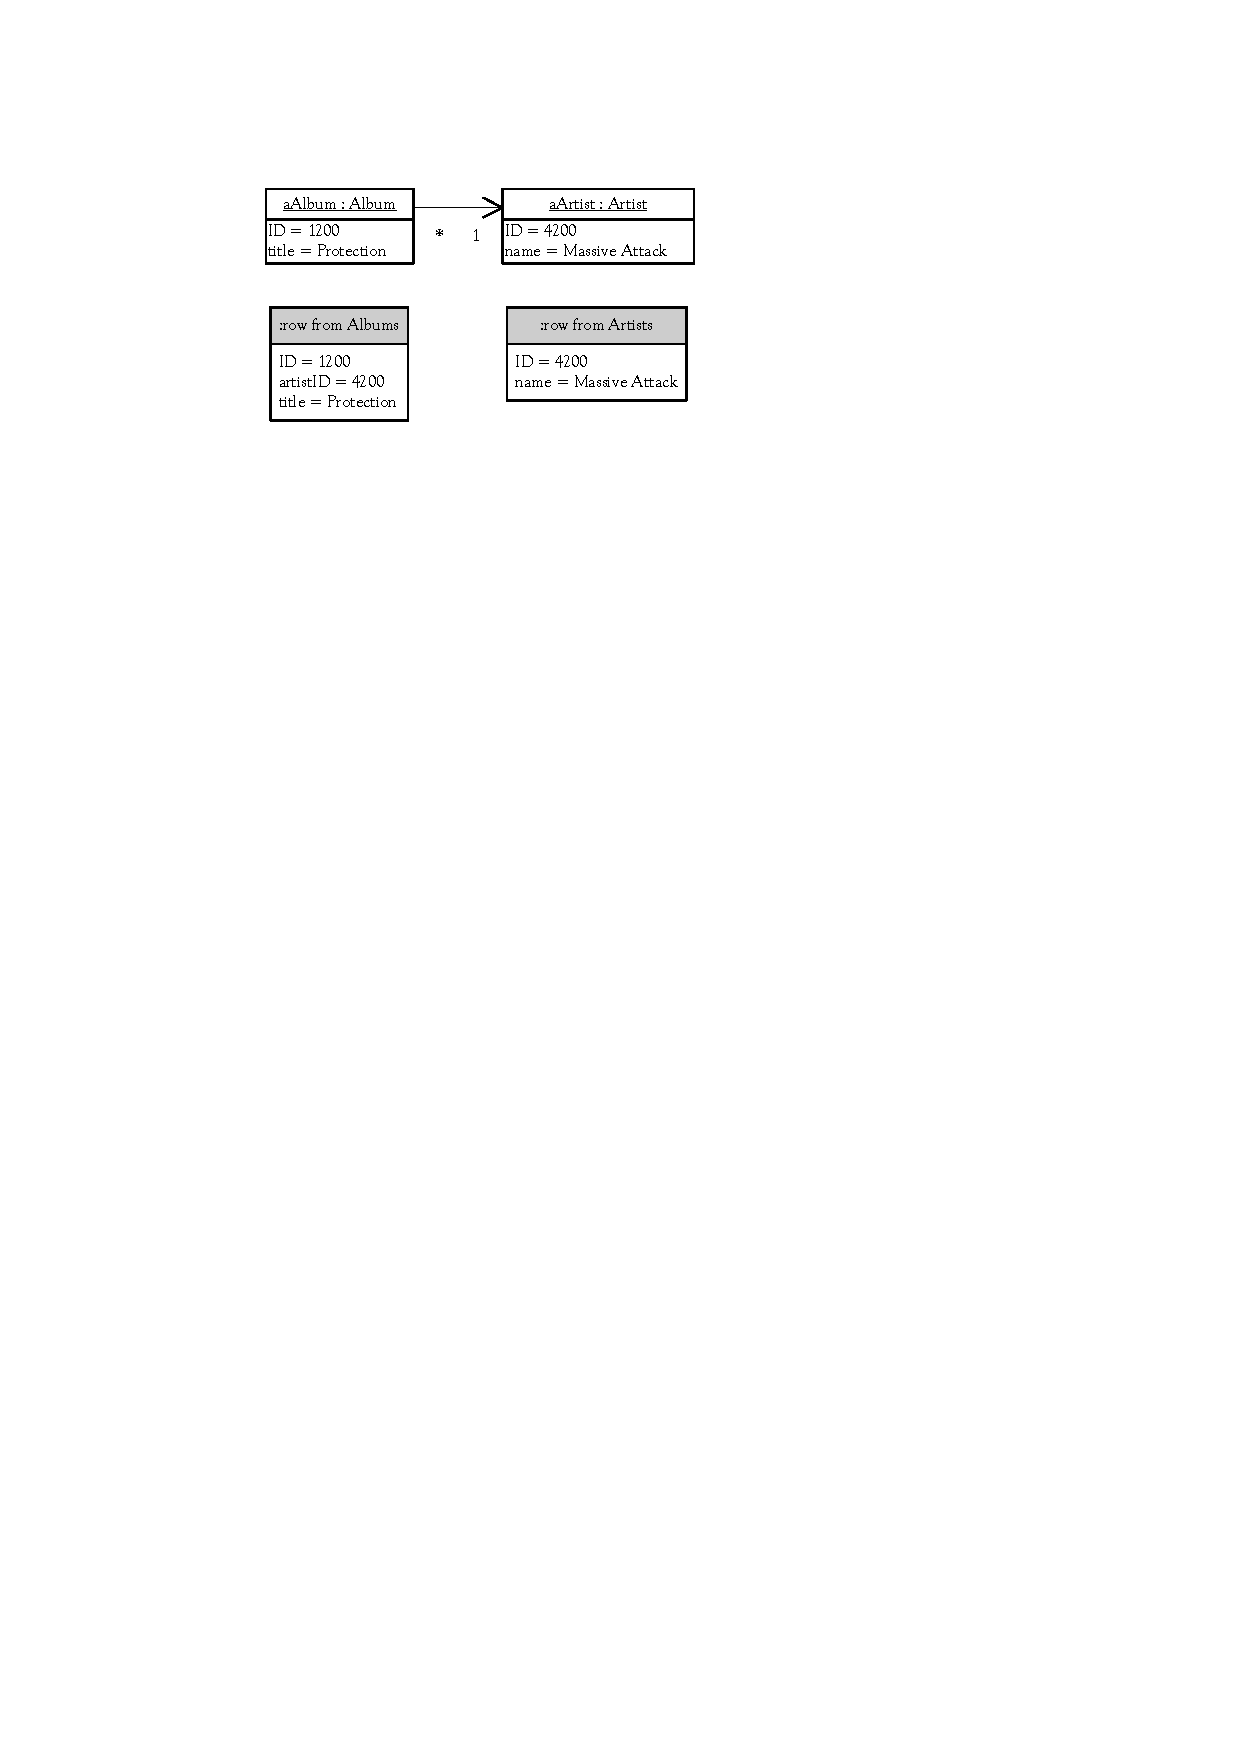
\includegraphics{./files/inc/figures/patternsForeignKeyMapping1}
					\caption{\label{fig:patternsForeignKeyMapping1} Simple Foreign Key Mapper}
				\end{center}
			\end{figure}
			Things get more complicated when one has to keep track of a collection of objects, because
			a collection cannot be saved to a database. The direction of the reference needs to be reversed.
			In our example, which is shown in Figure \ref{fig:patternsForeignKeyMapping2}, this means to
			store a foreign key of the album in the track record.

			\begin{figure}[htb]
				\begin{center}
					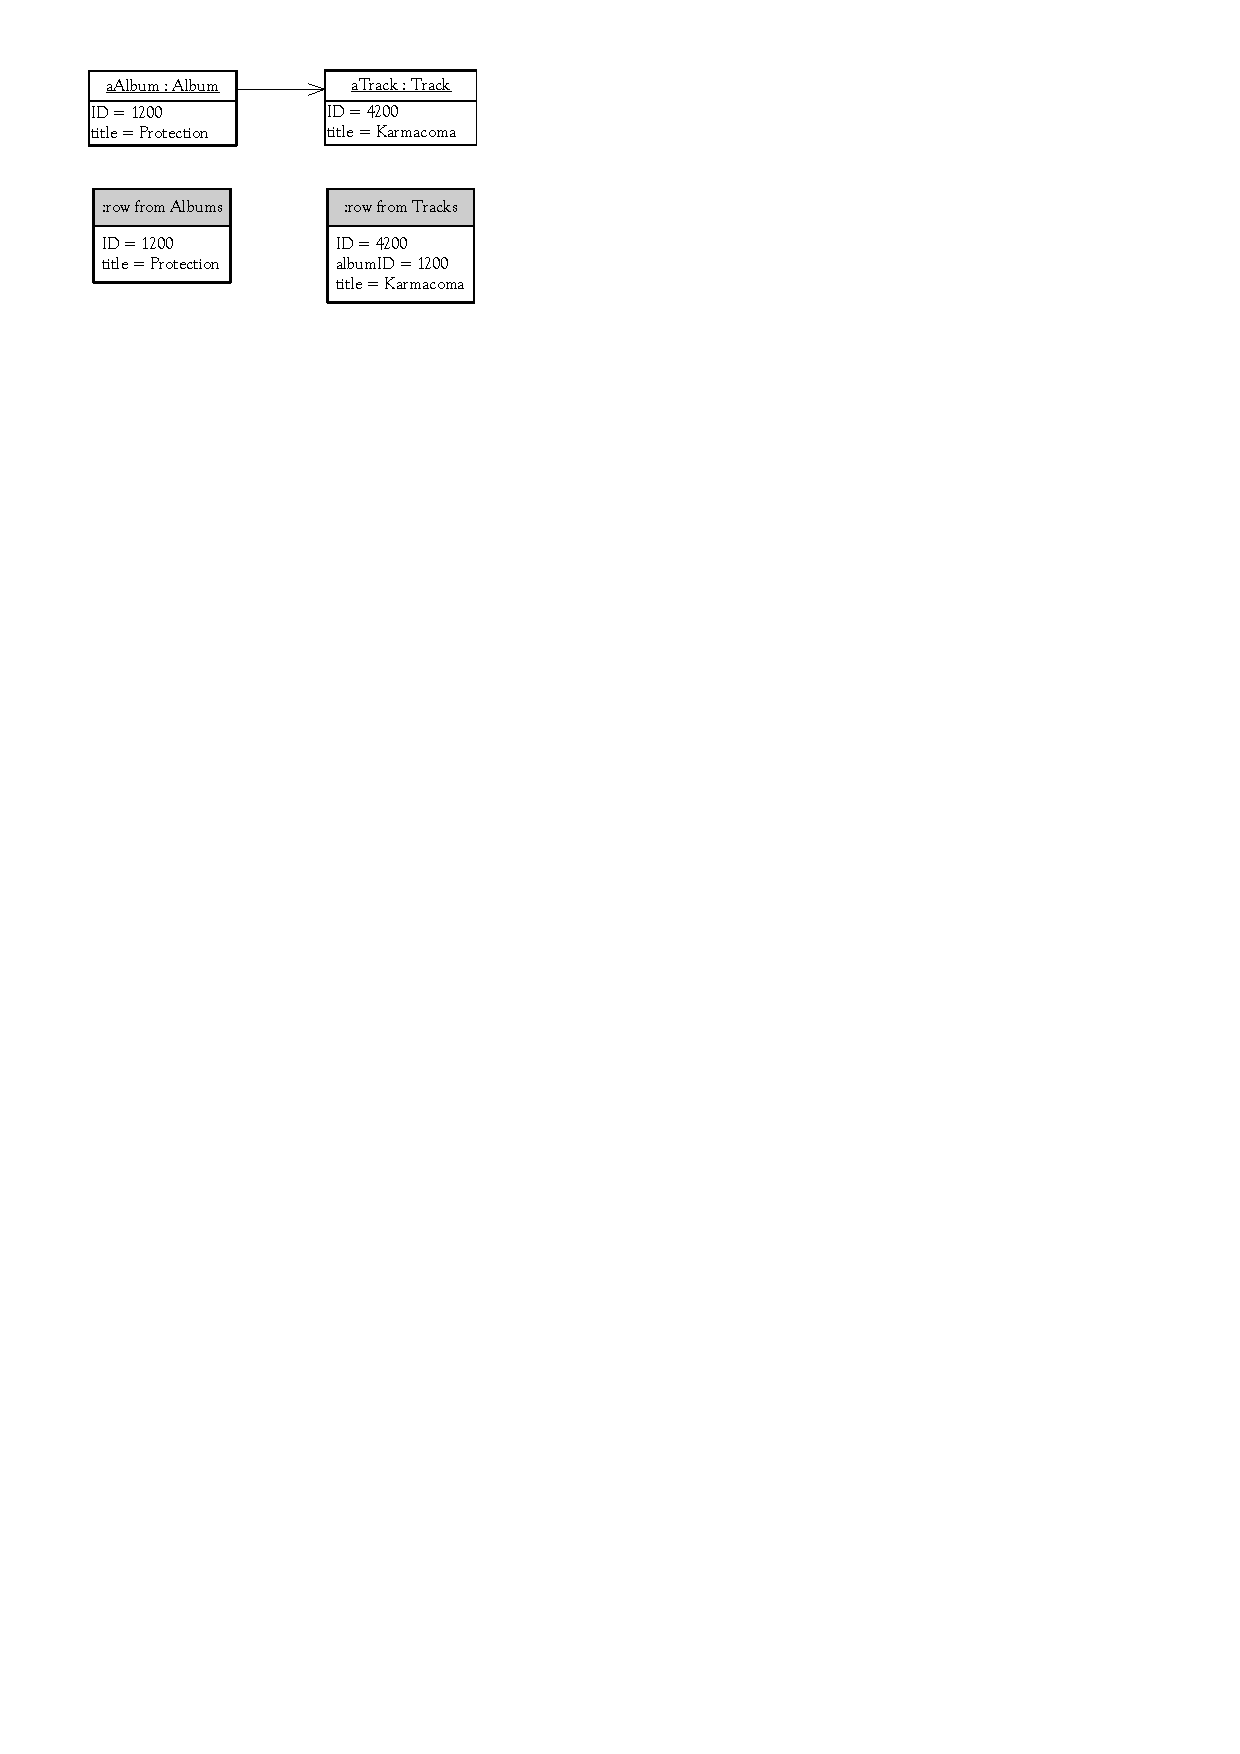
\includegraphics{./files/inc/figures/patternsForeignKeyMapping2}
					\caption{\label{fig:patternsForeignKeyMapping2} Mapping a collection to a foreign key}
				\end{center}
			\end{figure}
			This pattern needs to be discussed in more detail, especially cases where one needs
			to update a collection objects. This will be explained in the appropriate section, where
			implementation details are subjected.
			
		\subsection{Identity Field}
		\label{subsec:identityField}
			A relational database distinguishes one row from another by using keys. A key usually
			is nothing else than a \verb~long~ data-type. However, in-memory objects do not have such 
			key (it is the systems responsibility to keep track of object identities). Reading from a
			database is never a problem where database keys are concerned, writing is a problem though.
			One needs to save a copy of the database key in the in-memory object to tie this object to
			the corresponding database row. The \textit{Identity Field} pattern should be used whenever a mapping between
			in-memory objects and rows in a database is needed (which is almost always).
			
		\subsection{Metadata Mapping}
		\label{subsec:metadataMapping}
			As already mentioned, in-memory objects and database rows have different mechanisms to
			organise and structure data. Mapping this structures is what object-relational Mapping 
			is all about. To achieve this, many lines of code are needed to describe how fields in
			the database correspond to fields in in-memory objects. The resulting code
			is repetitive to write. With a code generation tool (in this case OOXGen - which is a result of this 
			thesis) a \textit{Metadata Mapping} pattern can be used to generate those repetitive lines of code.
			The input of the OOXGen is the metadata and the output is the source code of classes that do 
			the mapping. On most occasions the metadata is kept in a separate file, such as an XML file or
			even in the database itself. Figure \ref{fig:patternsMetadataMapping} shows the principle of the
			\textit{Metadata Mapping} pattern.
			
			\begin{figure}[htb]
				\begin{center}
					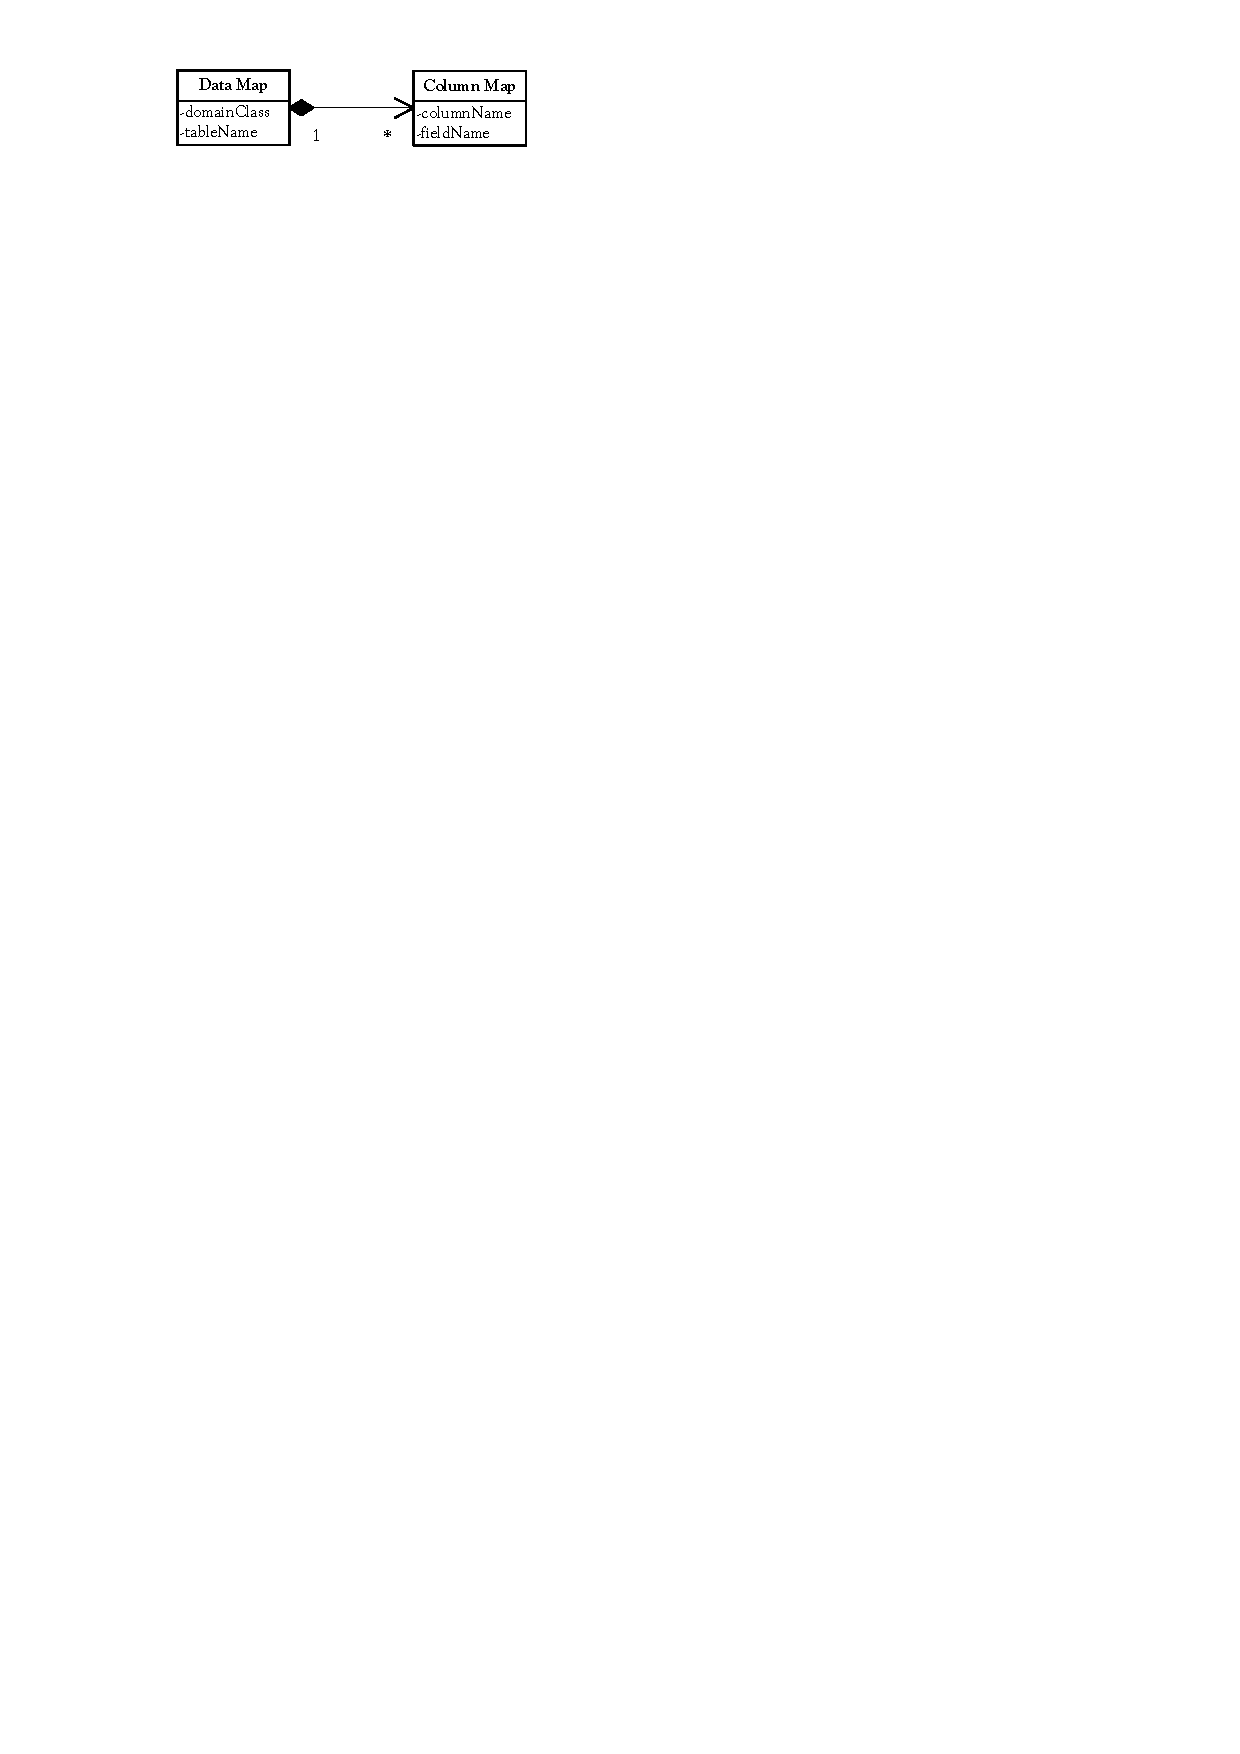
\includegraphics{./files/inc/figures/patternsMetadataMapping}
					\caption[Metadata Mapping principle]{\label{fig:patternsMetadataMapping} Holds details of object-relational mapping in metadata}
				\end{center}
			\end{figure}
			
		\subsection{Query Object}
		\label{subsec:queryObject}
			A \textit{Query Object} is a structure of objects that can form itself into a SQL query.
			A query can be formed by referencing classes and fields rather than tables and columns. 
			This allows a client to form a query of various kinds and turn those object structures into
			the appropriate SQL statement.
			With \textit{Query Object} you can separate SQL statements from the rest of the code
			which makes it possible to use different objects for different database schemata. This
			can be very powerful and makes code more readable. Furthermore a developer needs
			to know neither the details of the database nor he needs to be familiar with the SQL language.
			Figure \ref{fig:patternsQueryObject} shows an example of a possible \textit{Query Object}.
			
			\begin{figure}[htb]
				\begin{center}
					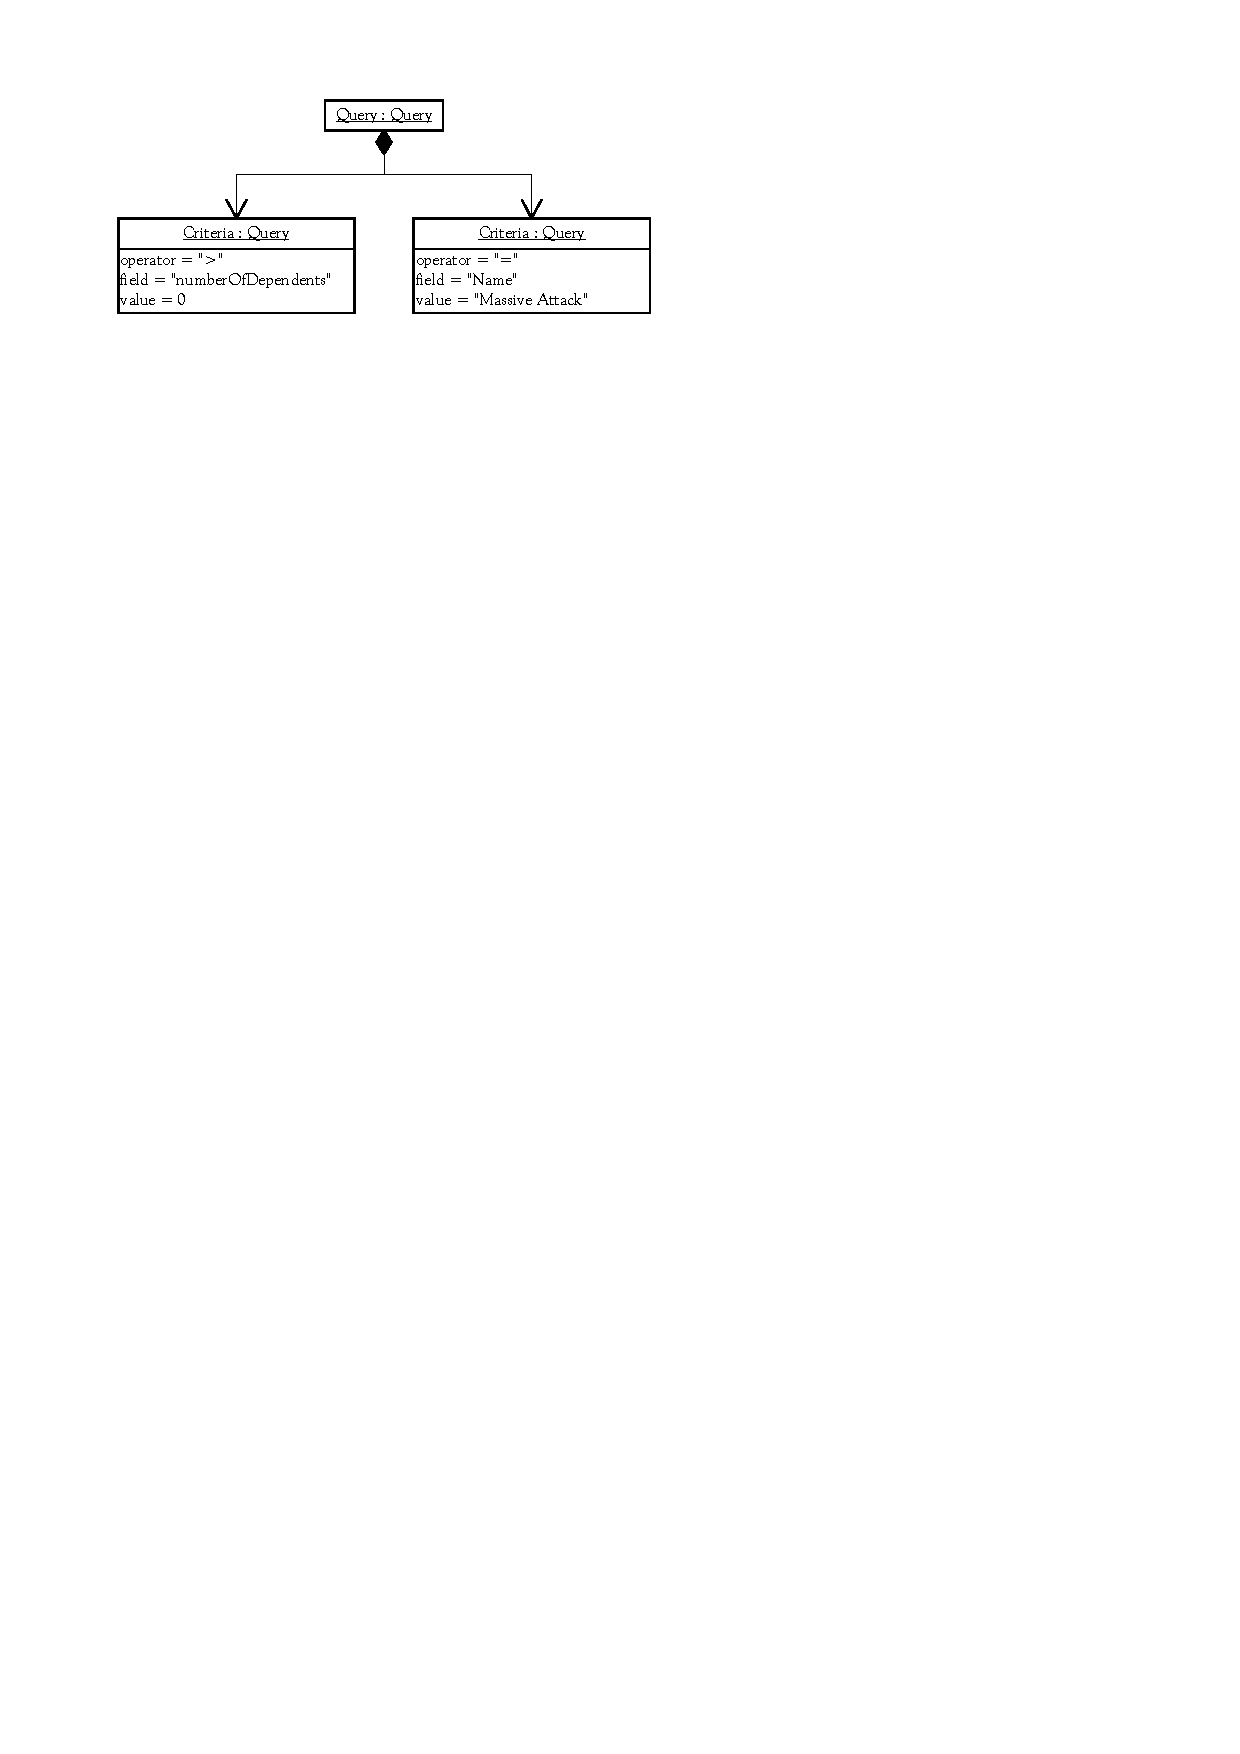
\includegraphics{./files/inc/figures/patternsQueryObject}
					\caption{\label{fig:patternsQueryObject} An Object Query representing a database query}
				\end{center}
			\end{figure}
			
		\subsection{Repository}
		\label{subsec:repository}
			A \textit{Repository} is a separation Layer between domain objects and a \textit{Data Mapper}.
			It isolates domain objects from details of the database access code. 
			Conceptually, a \textit{Repository}
			encapsulates the set of objects persisted in a data store and the operations performed over them.
			It presents a simple interface for clients which can create a Criteria object specifying
			the characteristics of the objects they want returned from a query. These Criteria Objects
			are submitted to the \textit{Repository} for satisfactory. In conjunction with 
			\textit{Query Object}, this pattern adds a large measure of 
			usability to the object-relational mapping layer. Client code do not need to use a \textit{Query Object}
			directly, instead it creates criteria objects and passes them to the \textit{Repository}, asking it 
			to select those objects that match.
			
		\subsection{Remote Facade}
		\label{subsec:remoteFacade}
			A remote call is always very expensive in terms of performance. It is better to do things in a
			single call rather than multiple calls. This is opposed to local calls. A \textit{Remote Facade}
			provides a coarse-grained interface for remote calls. This principle is illustrated in Figure
			\ref{fig:patternsRemoteFacade}. Rather than making a remote call for each element in an address,
			one call for all elements is performed. Therefore, this pattern describes the principle
			of designing coarse-grained interfaces which remote clients, such as web-services, can use.
			This pattern is a special \textit{Facade} which is described in E. Gamma's Design Patterns \cite{Gamma97}.
			A \textit{Facade} generally provides a simplified, standardised interface to a large set of objects.
			
			\begin{figure}[htb]
				\begin{center}
					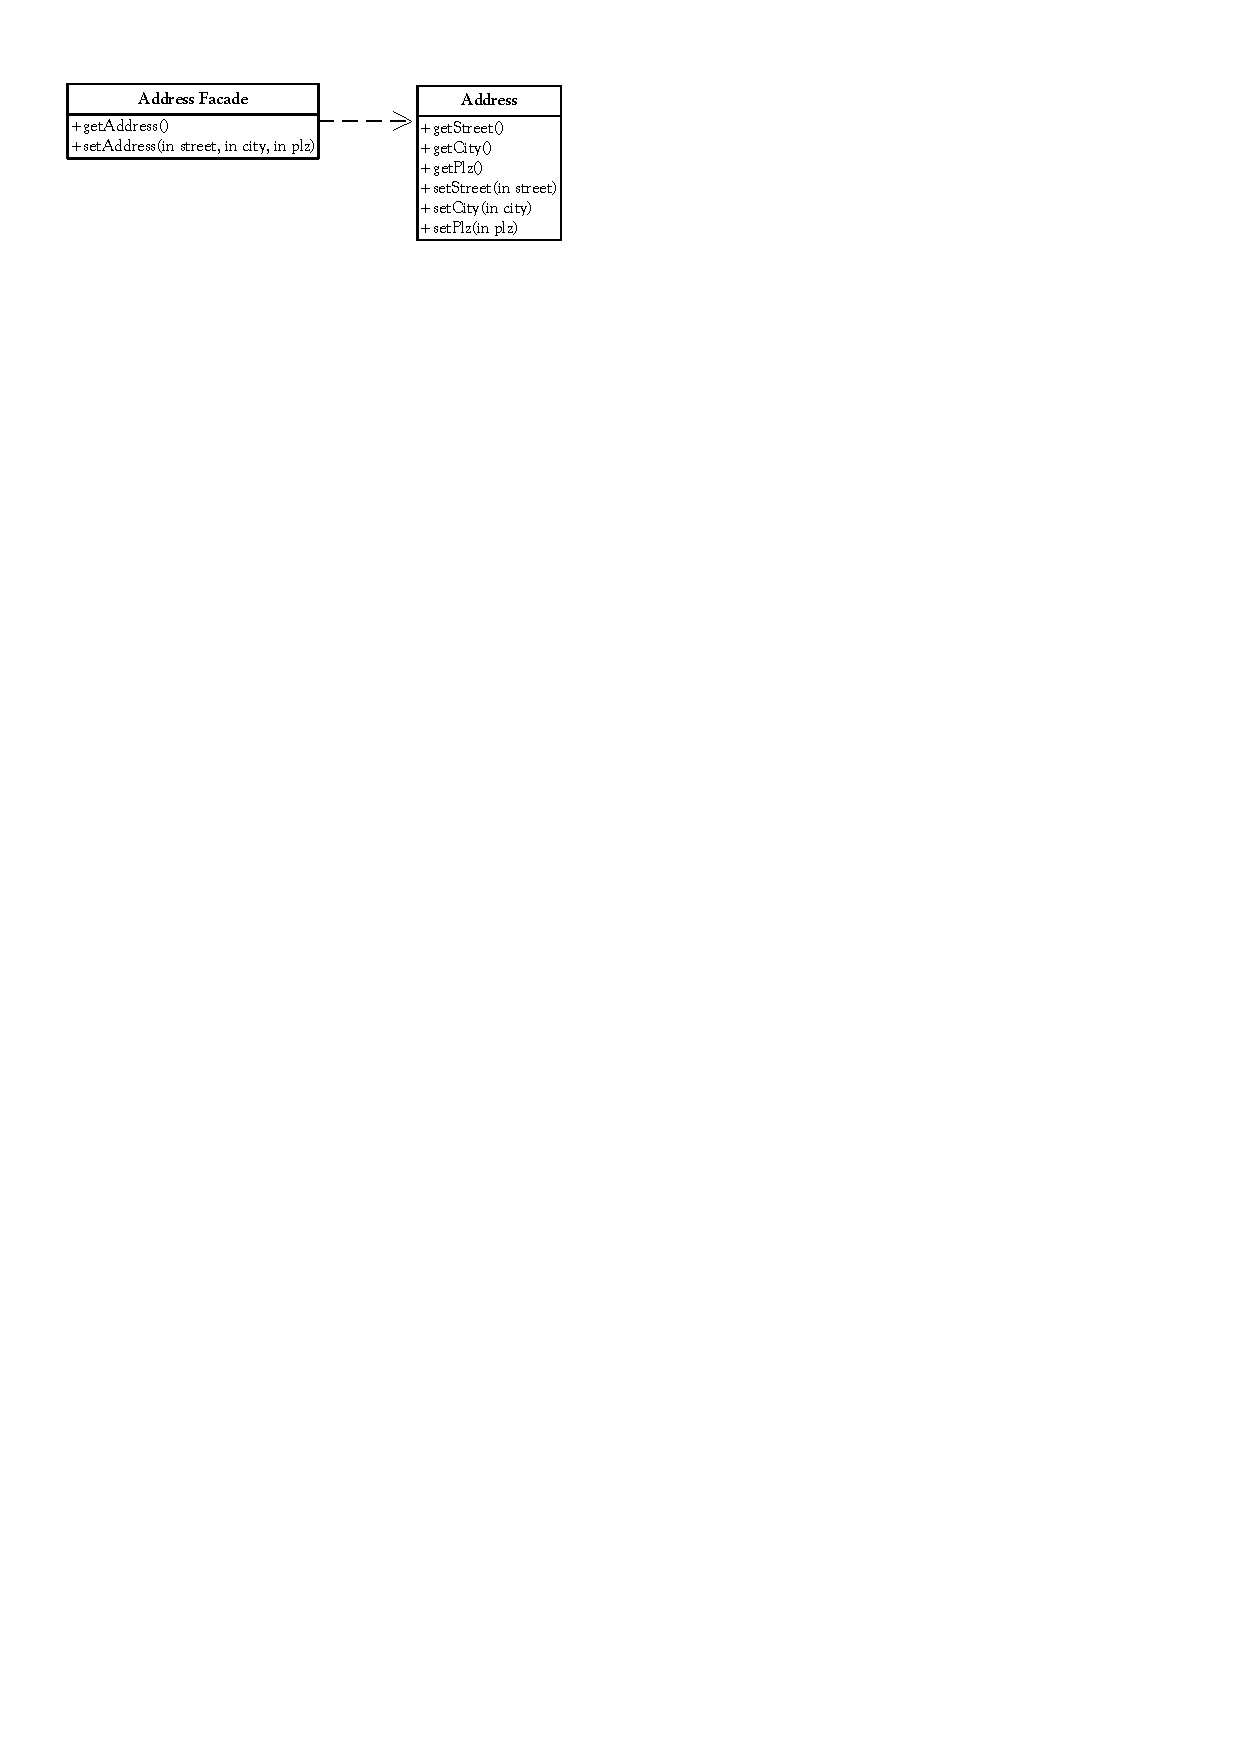
\includegraphics{./files/inc/figures/patternsRemoteFacade}
					\caption{\label{fig:patternsRemoteFacade} A coarse-grained remote call}
				\end{center}
			\end{figure}
			
		\subsection{Optimistic Offline Lock}
		\label{subsec:optimisticOfflineLock}
			A business transaction often includes a series of transaction. A single transaction
			is locked by the database manager. That is, no other transaction can access the same
			data at the same time. When you have more than a single transaction, you need a mechanism 
			to ensure that data at the end of a business transaction is in consistent state. This
			can be done with locks.
			There are two different approaches how a transaction can obtain a lock. This is
			either pessimistic or optimistic offline lock. The main difference is that \textit{Pessimistic
			Offline Lock} assumes that the chance of session conflict is high whereas \textit{Optimistic Offline
			Lock} assumes that the chance of one transaction conflicts with another is low. \textit{Pessimistic
			Offline Lock} is easier to implement but it limits system concurrency. This is because at a given time
			only one user can work with the locked data. \textit{Optimistic Offline Lock} allows multiple users to
			work with the same data at the same time. This is often very desirable but means to solve some problems
			which can occur when multiple users change data at the same time. Namely this problems are with
			\verb~UPDATE~ and \verb~DELETE~ SQL statements. Additionally, inconsistent reads must be detected.
			
			An \textit{Optimistic Offline Lock} is obtained by validating that, in the time since a transaction session loaded a
			record, another session has not altered it. This is usually done by comparing a version number
			stored in a session with the version in the record data.
			Figure \ref{fig:patternsOfflineLock} shows an \verb~UPDATE~ with \textit{Optimistic Offline Lock}. The version
			number is checked within the \verb~UPDATE~ statement and a row count of $1$ is returned in case of
			success otherwise a row count of $0$ is returned. An example of \textit{Optimistic Offline Lock} is 
			the concurrent versions system (CVS).
			
			\begin{figure}[htb]
				\begin{center}
					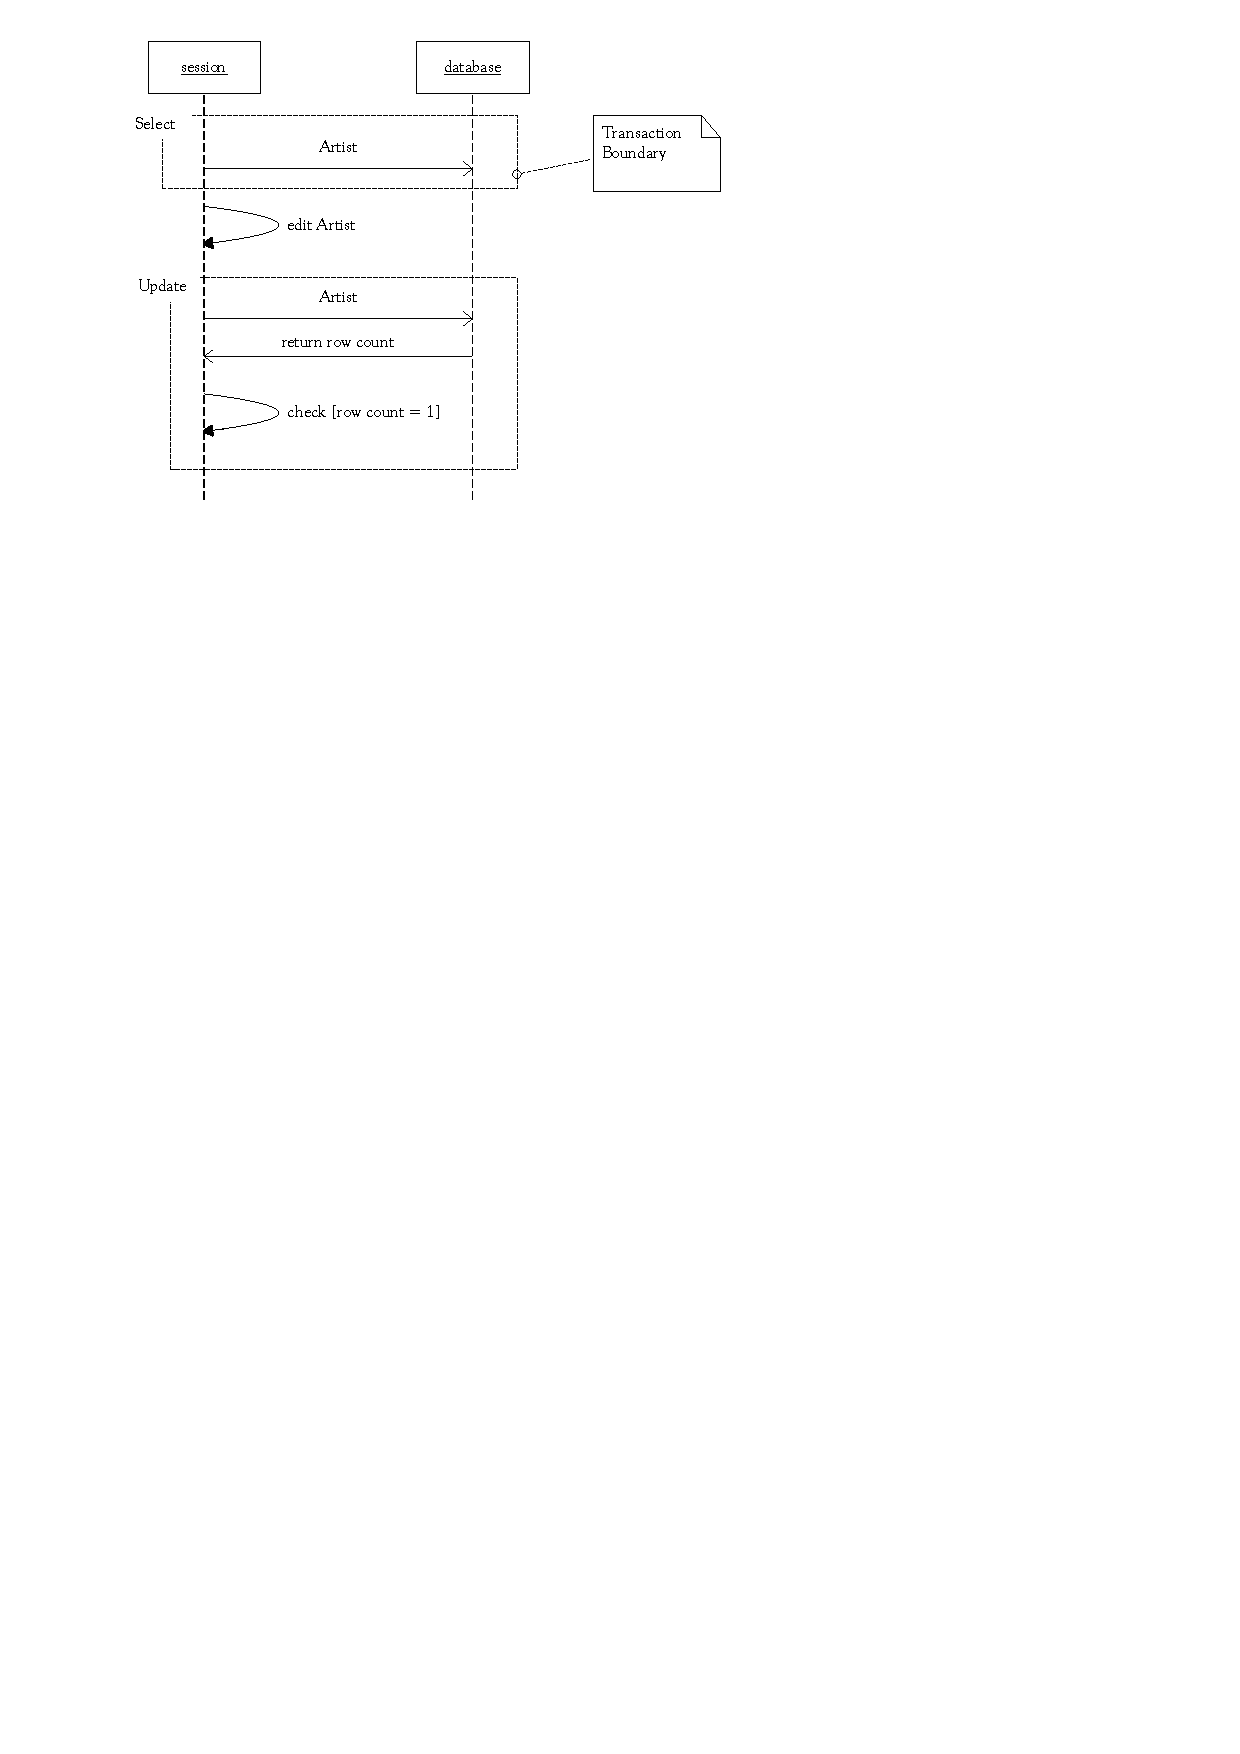
\includegraphics{./files/inc/figures/patternsOfflineLock}
					\caption{\label{fig:patternsOfflineLock} UPDATE with Optimistic Offline Lock}
				\end{center}
			\end{figure}
			Checks for inconsistent reads can become very tricky even with a few transactions. A 
			solution can be to group together transactions which depend on each other. This group 
			can be treated as a single lockable item.
			
		\subsection{Layer Supertype}
		\label{subsec:layerSupertype}
			The \textit{Layer Supertype} pattern describes the idea of an interface. An interface acts
			as a superclass which defines all common methods. Each class which references this 
			interface independently implements these methods.

			This way of implementing common features is very widespread in object-oriented
			programming and is therefore not explained in more detail.

		\subsection{Mapper}
		\label{subsec:mapper}
			A \textit{Mapper} is a layer between subsystems. It decouples these subsystems from each other. When
			using a \textit{Mapper}, either subsystem is not aware of the other but they still can communicate
			through the \textit{Mapper}. The most common case of a mapping layer is a \textit{Data Mapper}
			(\ref{subsec:dataMapper}).
				
		\subsection{Registry}
		\label{subsec:registry}
			A \textit{Registry} is essentially a global object. If you have methods for which
			you do not have a reference to start with, you can register this methods in a
			\textit{Registry}. A \textit{Registry} is usually implemented as a singleton class. This 
			makes it possible to get access to those methods from within the whole program. There are
			always workarounds in case you do not like to use a \textit{Registry}.
			
		\subsection{FactoryMethod}
		\label{subsec:factoryMethod}
			A \textit{Factory Method} defines an interface for creating an object. Which object
			is to be created is decided by subclasses. Usually a \textit{Factory Method} is needed
			when a class cannot anticipate the class of objects it must create. This is often the
			case with frameworks which must provide a mechanism to create concrete implementations
			of abstract classes. A framework does not know at design time which classes this will be.
			The idea is to pass all needed information to the \textit{Factory Method} which in turn
			will create the object. The advantage is to eliminate the need to bind application-specific
			classes into the code.
			The design of a \textit{Factory Method} is shown in Figure \ref{fig:patternsFactoryMethod}.
			
			\begin{figure}[htb]
				\begin{center}
					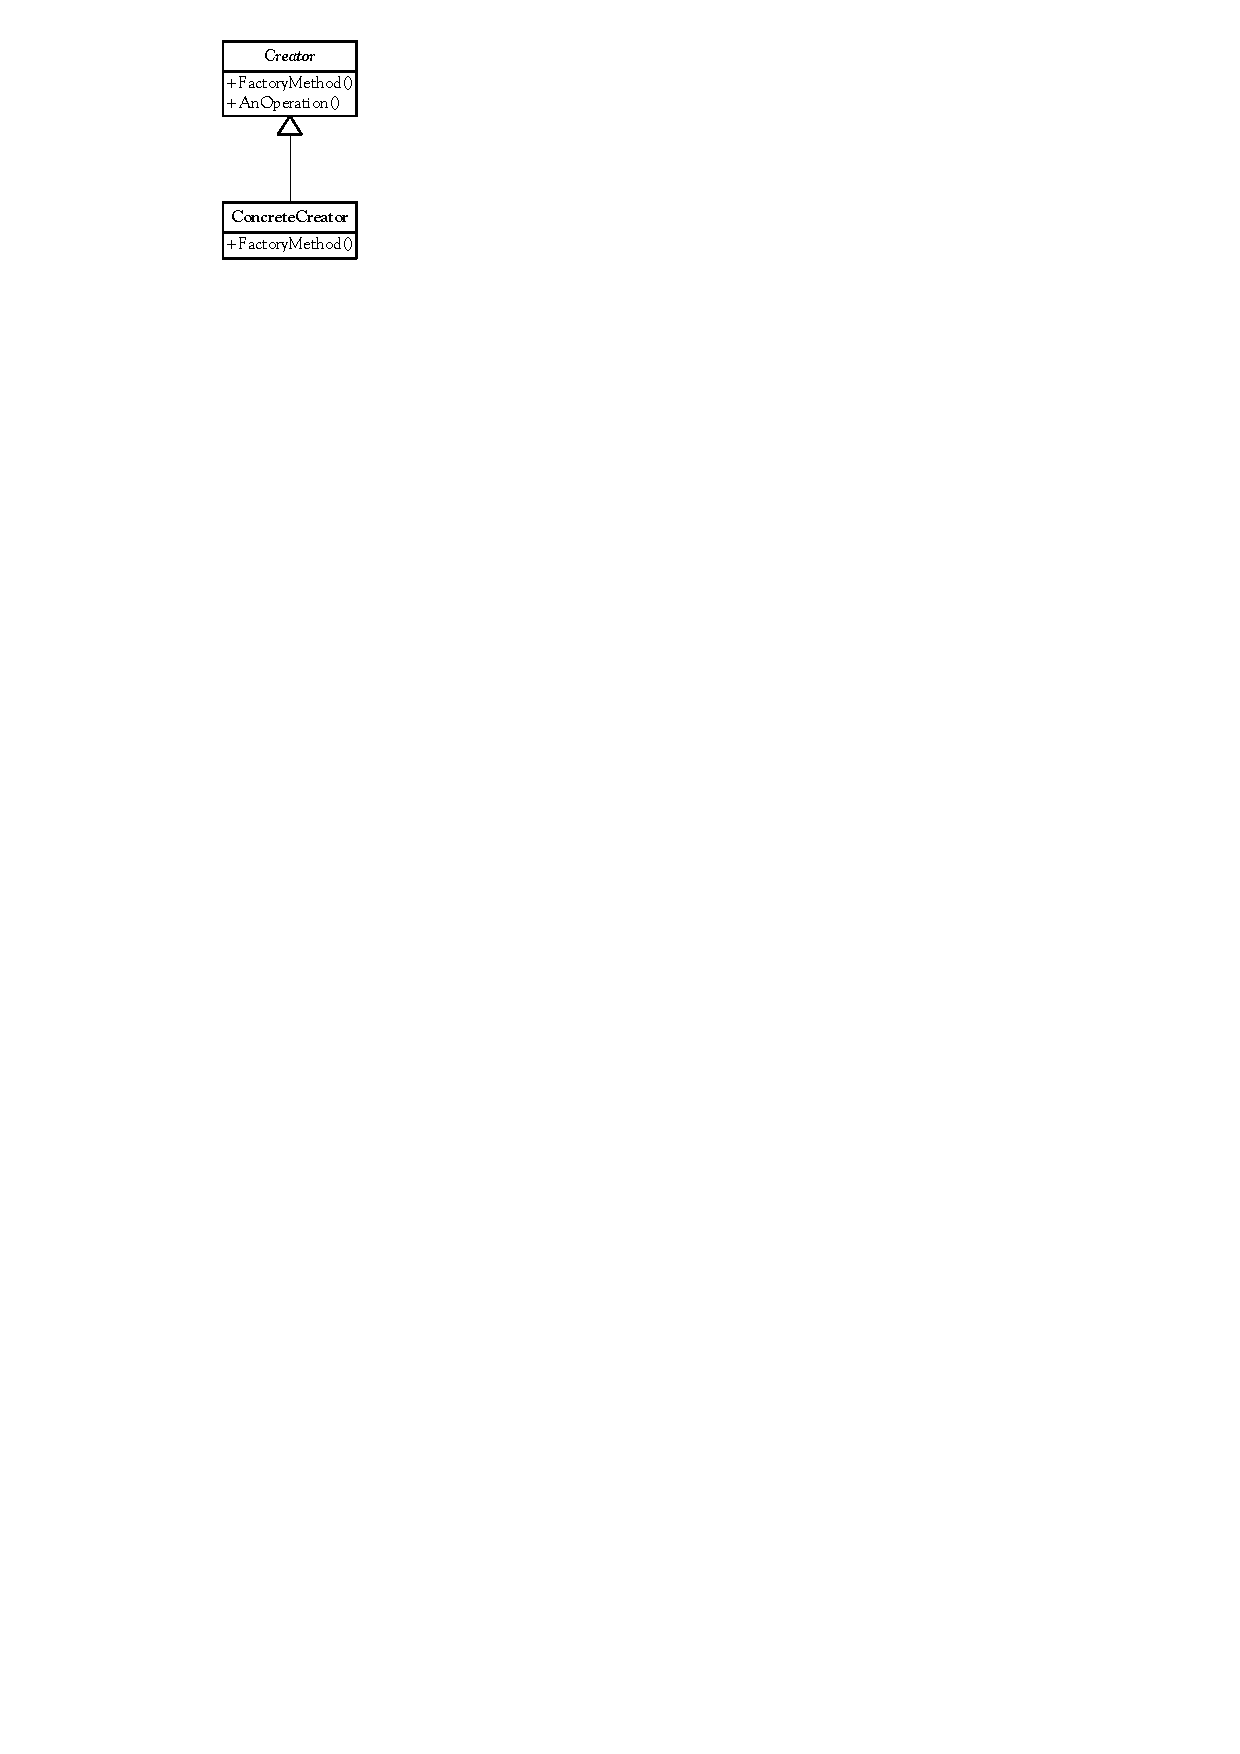
\includegraphics{./files/inc/figures/patternsFactoryMethod}
					\caption{\label{fig:patternsFactoryMethod} Factory Method Design}
				\end{center}
			\end{figure}

			
		\subsection{Separated Interface}
		\label{subsec:separatedInterface}
			A design paradigm is to decoupling individual parts of the system. A way to achieve this is
			to group classes in packages and control the dependencies between them. \textit{Separated Interface}
			is a way to manage these dependencies. You can define an interface in one package and put
			the implementation of this interface in a different package. This way, you do not have to
			reference classes in a different package, you only need a reference to the interface.
			A sample of this pattern is shown in Figure \ref{fig:patternsSeparatedInterface}
		
			\begin{figure}[htb]
				\begin{center}
					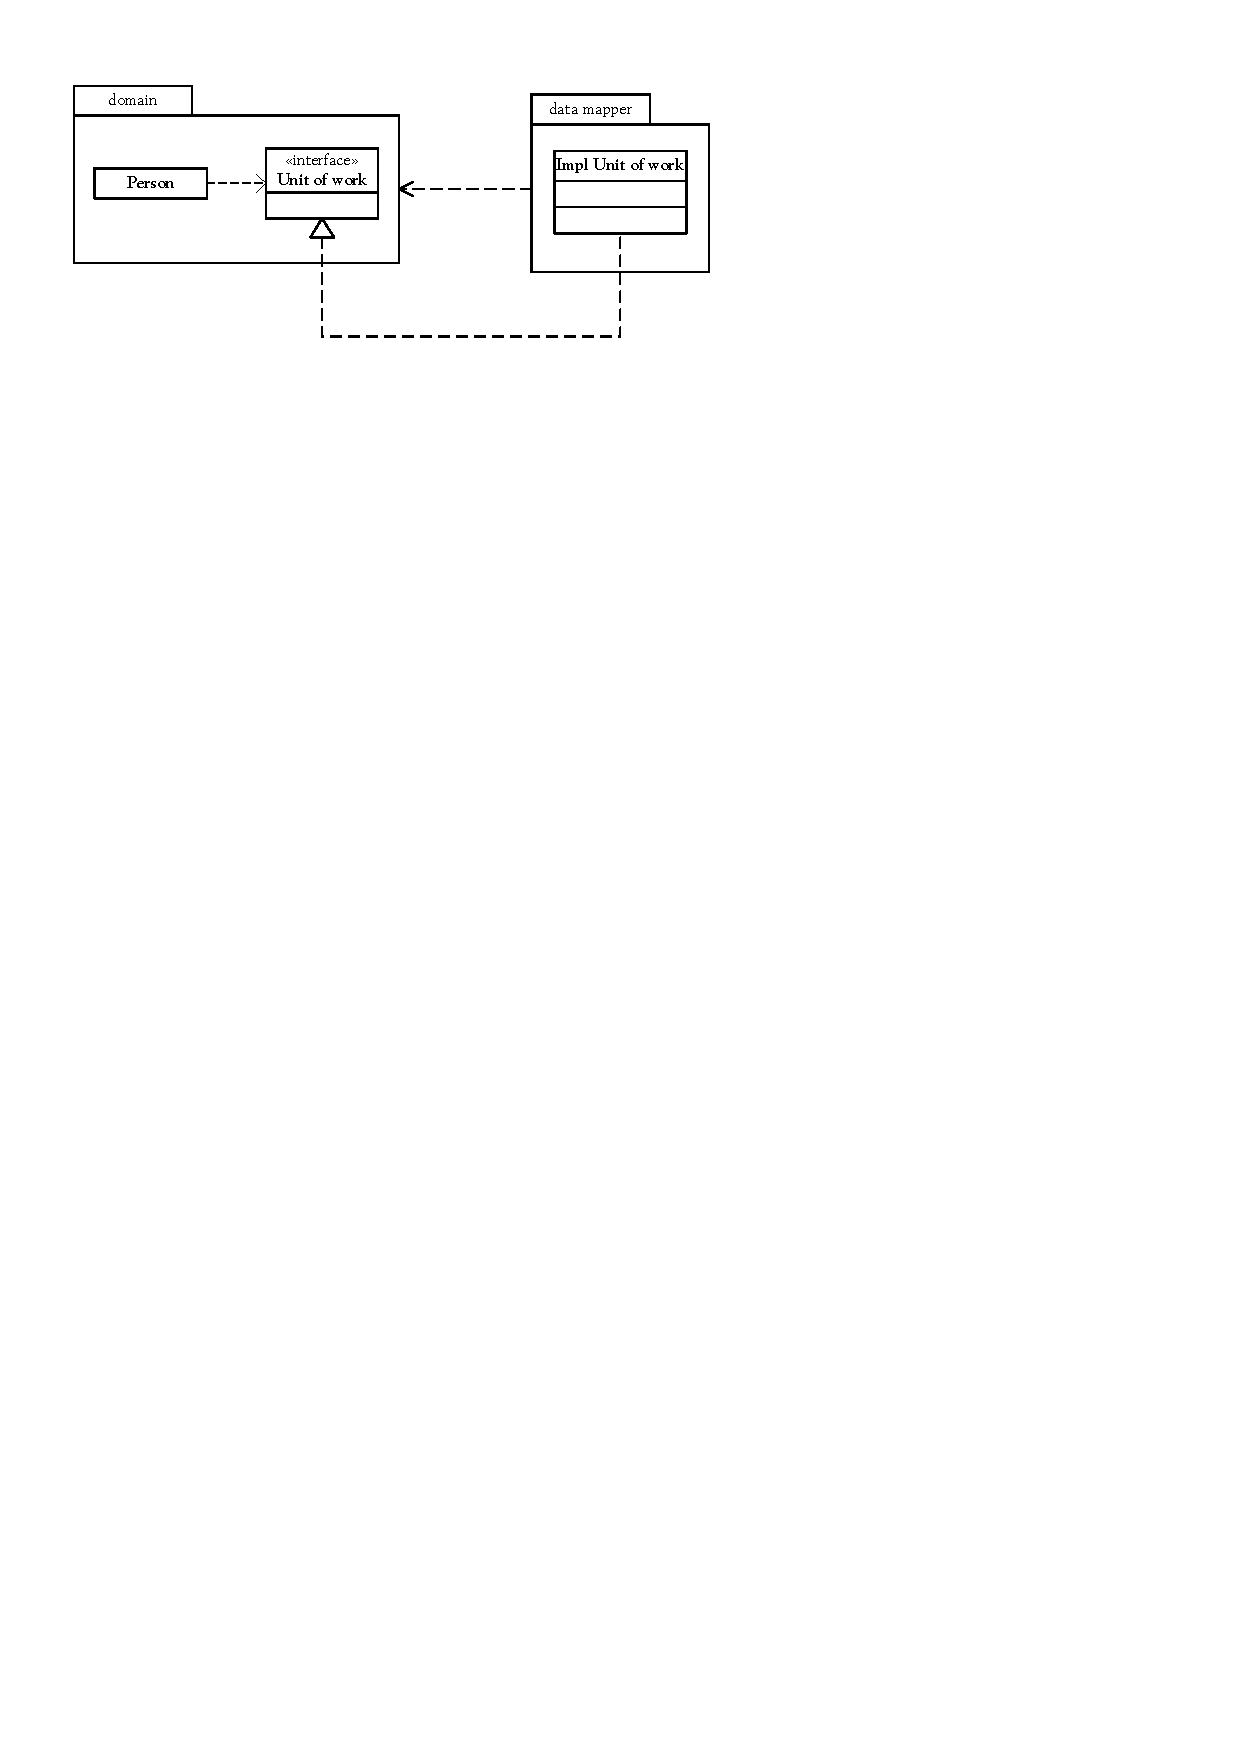
\includegraphics{./files/inc/figures/patternsSeparatedInterface}
					\caption{\label{fig:patternsSeparatedInterface} Sample of Separated Interface}
				\end{center}
			\end{figure}

%\chapter{Design Considerations}
\label{cha:designConsiderations}
	
	%----------
	\section{Fundamental Approach}
		\textit{STORM} is a framework to generate code for an object-relational mapper on
		basis of templates. There are a few question which need to be answered before starting
		a design for the framework. These questions are:
		
		\begin{enumerate}
			\item	What needs to be parameterised?
			\item How can parameters be defined?
			\item How can parameters be passed to templates?
		\end{enumerate}
		
		\subsection{What needs to be parameterised?}
			Obviously, for an object-relational mapper the most important thing to parameterise
			is the mapping. This means, the database structure, the structure of the in-memory objects
			and the mapping between them must be defined. For example, one needs to be able to define
			that an in-memory object of a class \verb~Person~ maps to a database table called \verb~Persons~.
			Not only the structure must be configurable but also primary keys,
			foreign keys and relations between tables.
		
		\subsection{How can parameters be defined?}
			After we know \emph{what} needs to be parameterised, the question is \emph{how}. At the beginning
			of this thesis, three different fundamental approaches were analysed and tested.
			
			The first approach is XML Schema: There are two XML Schema files and one plain XML file.
			One XML Schema file is to define the in-memory object structure, the other one is to define
			the database structure and the XML file is used to describe the mapping between the two.
			The problem of this approach is its complexity and unmanageability.
			
			Another approach was an extended C\# compiler. This compiler would work with custom defined
			keywords. This keywords could be used to define the structures and mapping.
			
			The third approach to describe the mapping is to write an abstract class
			with custom attributes. A code snippet of such a class is shown in Listing
			\ref{lst:abstractClassAdr}. After compiling this has been compiled, the custom
			attributes can be read using reflection from the resulting dll. With these attributes,
			all relevant information can be retrieved.
			
					\begin{lstlisting}[float=htb,language={[Sharp]C},caption=Abstract class with custom attributes,label=lst:abstractClassAdr]
	[Table("Addresses", true),
	VersionField("chTimeStamp"),
	GenerateCode]
	public abstract class Address : DomainObject
	{
		[Factory]
		public abstract class AddressFactory
		{
			public abstract Address createAddress(
			[ParameterDef("City")] string city,
			[ParameterDef("Street")] string street,
		}

		[Column("AddressID"),
		PrimaryKey]
		public abstract int AddressId {get;}

		[ToMany(typeof(OrderDetail), "OrderId")]
		public abstract IList OrderDetails {get;}

		[Column("PersonID"),
		ToOne(typeof(Person), "PersonId")]
		public abstract Person PersonRel {get; set;}

		[Column("City")]
		public abstract string City {get; set;}

		[Column("Street")]
		public abstract string Street {get; set;}
	}
}
			\end{lstlisting}
			
			The main advantage of this is that a programmer can define everything in a single file (single-source approach)
			rather than multiple files. This means, not only the mapping code could be generated automatically, but also
			the corresponding database tables. Furthermore it is a natural way for programmers because
			they are used to write classes.
			
			One could say that a drawback of attributes is that they cannot be changed at runtime.
			This is true but also, it is not required. Every information given in this 
			abstract class is static within the scope of an application. 
			
			From our point of view, this approach is the most feasible. 
			
		\subsection{How can parameters be passed to templates?}
			Once we know how to parameterise everything we need a way to let the 
			template know all these parameters. The first thing which is given is that
			custom attributes in C\# are bound to the class in in which they are defined.
			Therefore, attributes must be read by using reflection. First, we could
			generate code which makes use of reflection or second, we use reflection
			in the template itself an generate code containing no reflection but the 
			concrete code resulting from the custom attributes. The latter case is more
			according to the idea of generative programming. If we used reflection
			in the generated code the application's performance would be poorer. What is more,
			it would not make much sense because we would not need to write any templates
			at all.
								
	%----------
	\section{Object Dependencies}
		Whenever code is generated, it is important to design the application carefully.
		An important consideration must be object dependencies. This is, an abstract class or any
		class written in the client code
		may never depend on a generated class nor may a generated class depend on
		another generated class. If such a dependency existed, it would result in a dependency
		cycle which cannot be resolved. Consider an abstract class \verb~Person~ which results
		in the concrete implementation class \verb~PersonImpl~. Further, consider a client 
		which wants to set the property \textit{Name} for a \verb~Person~ and uses the concrete
		implementation \verb~PersonImpl~ for this (see Figure \ref{fig:DesignObjectDependency}). This
		would have the effect that the client class could not be compiled before the concrete
		implementation is generated. But to generate the concrete implementation, the client code
		needs to be compiled (because the resulting dll is needed). This could be avoided by putting
		the client code in a separate project. But at the latest when you have dependencies between
		abstract classes and concrete implementation classes this cannot be avoided.
		
		Therefore a mechanism is needed that the client code just need to reference the 
		abstract class but still can set the property in the concrete implementation object.
		For this we use a \textit{Factory Method} which provides us with a concrete implementation without
		the need of referencing it directly. How exactly the \textit{Factory Method} was used is explained
		in \ref{sec:Factory}.
		
		\begin{figure}[htb]
			\begin{center}
				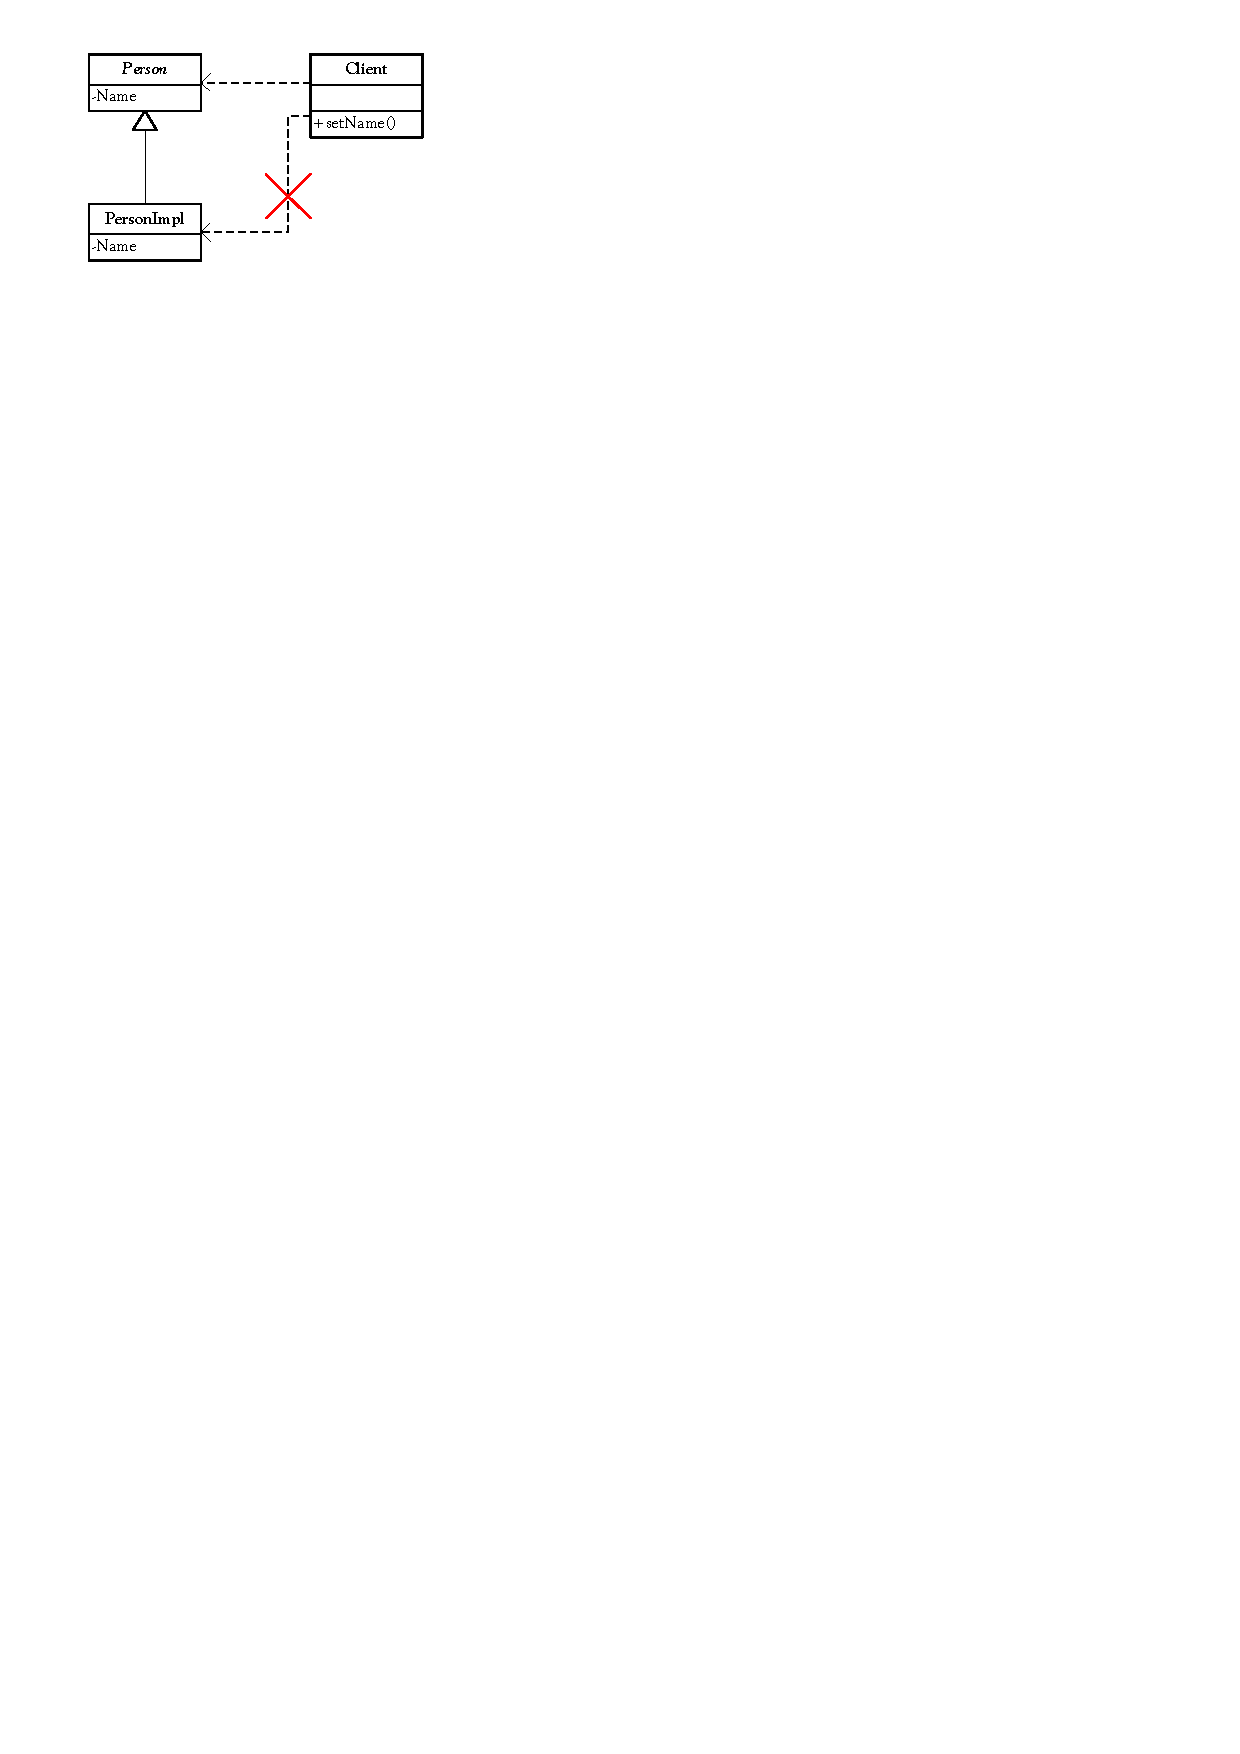
\includegraphics{./files/inc/figures/DesignObjectDependency}
				\caption{\label{fig:DesignObjectDependency} Dependencies between classes}
			\end{center}
		\end{figure}

	%----------
	\section{Object Lifetime}
	\label{sec:objectLifetime}
		An object which has been transferred from the database can be kept for further use in
		an \textit{Identity Map} (see \ref{subsec:identityMap}). The question is, how long this object resides in this
		map. An \textit{Identity Map} is stored in a \textit{Unit of Work} (see \ref{subsec:unitOfWork}) and therefore, if the
		\textit{Unit of Work} object is destroyed, the \textit{Identity Map} and all objects
		stored in it will be destroyed too. This is indicated in Figure \ref{fig:designUoW_IdentityMap}.
		This brings up the question how long a \textit{Unit of Work} object should exists. There are
		two answers for that:
		\begin{itemize}
			\item The objects lifetime is as long as a user session exists. This is, a \textit{Unit of Work}
						object is created on a per thread basis. A new thread is started on each new session.
			\item The object is on a per transaction basis. This is, a new \textit{Unit of Work} object is 
						created on every commit.
		\end{itemize}
		These two methods represent completely different concepts. The first implies that it is possible 
		for an object to reside in an \textit{Identity Map} for a long time. On the one hand, this increases the
		risk of consistency errors but on the other hand, it follows more the idea of an \textit{Optimistic
		Offline Lock} (see \ref{subsec:optimisticOfflineLock}) architecture. This means that
		consistency errors will rarely occur.
		Additionally, we avoid consistency errors by using a lazy load
		system which checks if the object in question is up to date (see \ref{subsec:LazyLoad}).
		
		The second method is more adequate for a system with many users who are likely to
		edit the same object simultaneously. In such
		systems, consistency errors are likely to occur. Whenever this is the case, it makes not
		much sense to store objects in an \textit{Identity Map} for a long time to just remove
		them upon the next update.
		
		We assume that the first case is more appropriate in most cases and use therefore a per
		session based \textit{Unit of Work}.
		
		\begin{figure}[htb]
			\begin{center}
				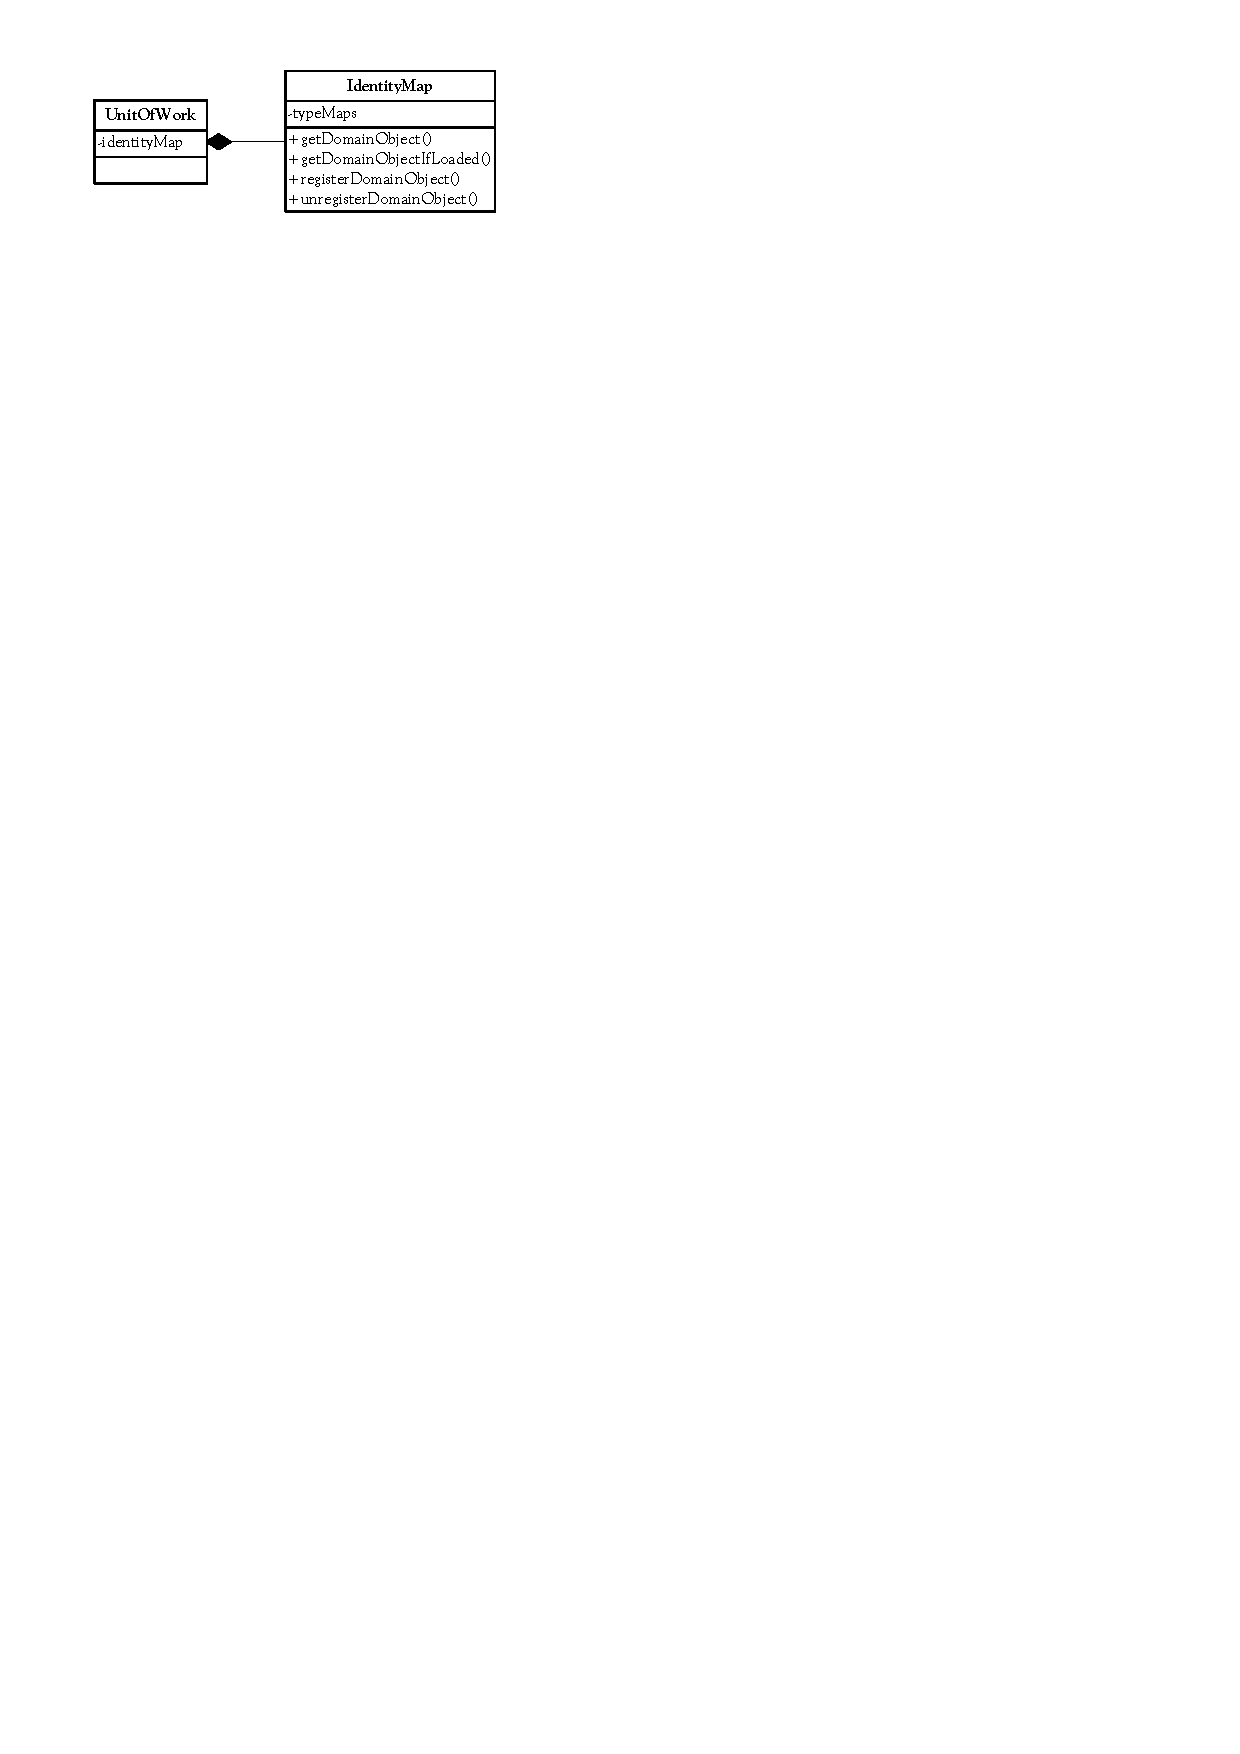
\includegraphics{./files/inc/figures/designUoW_IdentityMap}
				\caption{\label{fig:designUoW_IdentityMap} Relation between \textit{Unit of Work} and an \textit{Identity Map}}
			\end{center}
		\end{figure}
		
	%----------
	\section{Locking Mechanisms}
	\label{sec:lockingMechanisms}
		Depending on the application, different database locking mechanisms are appropriate. There are two
		main ways how database locking can be implemented:
		
		\begin{itemize}
			\item	The whole database is locked during a transaction. 
			\item Only certain records of the database are locked during a transaction.
		\end{itemize}
		
		The first method its easier to implement and adequate for many applications. It locks the
		whole database within a business transaction. The disadvantage of this is that whenever several
		people access the same data within a business transaction, only one of them can commit without 
		a conflict. For all others, the transaction will fail.
		
		The second method solves this problem by using more sophisticated locks. Several strategies
		can be used:
		
		\begin{description}
			\item[exclusive write lock] A business transaction acquires a lock in order to edit session data. Reading 
																	these data is still possible.
			\item[exclusive read lock]	A business transaction is required to acquire a lock simply to load the record.
			\item[read/write lock]			A record cannot be write-locked if any other business transaction owns a
																	read lock on it and vice versa. Concurrent read-locks are acceptable.
		\end{description} 
		
		For this thesis, we use the first method which locks the whole database. The reason is that
		we do not have a concrete application for which a more complicated locking mechanism would
		be needed. But Generally, it is important to choose the right locking strategy.

	%----------
	\section{Mapping Types}
	\label{sec:mappingTypes}
		
		Not all possible mapping types are supported by \textit{STORM}. This section 
		describes the supported types. That is, which elements of the object oriented 
		code can be mapped to which database elements. The custom attributes which define
		the mapping is named for each type.
		A detailed description of the attributes can be found in section \ref{sec:attributes}.
		
		\begin{description}
			\item[Class]                     A class is always mapped to one table. Even though, it would be possible to map 
			                                 more than one class to the same table. 
			                                 
			                                 The \hyperlink{TableAttribute}{Table} attribute is mandatory for each class.
			\item[Member variable]           A member variable of a class is mapped to a column within 
			                                 the corresponding table.
			                                 
			                                 The \hyperlink{ColumnAttribute}{Column} attribute sets the name of the 
			                                 column.
			\item[One to one relation]       A relation from one table to exactly one entry of another table. Table 
			                                 $A$ contains the primary key or a unique key of an entry in table $B$.
			                                 In the source code, this mapping is done by referencing object $A$ to object $B$.
			                                 
			                                 \hyperlink{ToOneAttribute}{ToOne} is the attribute defining this relation.
			\item[One to many relation]      A relation from one table to several entries of another table. 
			                                 A database handles this relation by placing a foreign key in each entry
			                                 in table $B$. With this foreign key, entries in table $B$ know that they belong
			                                 to table $A$.

			                                 In the source code, object $A$ has an array list which contains all related 
			                                 objects $B$. \textit{STORM} needs a back reference (to-one relation) in class 
			                                 $B$ for each to-many relation in class $A$.
			                                 
			                                 \hyperlink{ToManyAttribute}{ToMany} is the attribute defining this relation.
			\item[Many to many relation]     To realise such a relation on the database, an 
				                               linking table is needed to store the relations between entries.

				                               In the code it is possible to manage many-to-many relations 
				                               with array lists without the need of an extra object between them.
				
				                               We do not support this special case. To make a many-to-many relation 
				                               it would be necessary to make an extra object which maps to the linking table.
				                               
			\item[Enumeration/Lookup tables] Enumerations are not needed and often not supported by 
				                               databases. If you are thinking about using an enum you should consider to save 
				                               the values in a lookup table. Enumerations are not supported by \textit{STORM}.
		\end{description}
		
		
%\chapter{Code Generation}
\label{cha:codeGeneration}

	%----------
	\section{Finding a Tool}
		Mainly two projects exist which are able to generate code on basis of templates. These are
		Workstate's Codify\footnote{\url{http://www.workstate.com/codify}} and 
		CodeSmith\footnote{\url{http://www.ericjsmith.net/codesmith/}}. Both projects were evaluated
		at the beginning of this thesis. CodeSmith has several advantages over Codify. First, it
		is open source and it seems that it has a bigger community. Moreover, it cannot only be
		integrated in Visual Studio .NET, it has a command line tool and it can be run 
		from the CodeSmith standalone program. Particularly the command line tool is
		useful for creating makefiles. Furthermore, CodeSmith has a much more powerful
		way to write custom templates. Therefore, the decision clearly felt on CodeSmith. 
		
	%----------
	\section{Procedure of Code Generation}
		To be able to customise CodeSmith templates,
		one needs parameters as input for them. Input parameters are in the case of \textit{STORM} the custom 
		attributes in the abstract classes. The procedure to actually generate the code is as follows:\\[2mm]
		
			\noindent
			\fbox{Parameterised, abstract classes}
				$\xrightarrow{\text{compile}}$ 
				\fbox{DLL}
				$\xrightarrow{\text{input}}$
				\fbox{Assembly Loader}\\[2mm]
				$\xrightarrow[\text{a given class}]{\text{read type of}}$
				\fbox{CodeSmith}
				$\xrightarrow[\text{of class}]{\text{read attributes}}$
				\fbox{Generated Code}\\[2mm]
				
		\noindent
		First, all abstract classes must be compiled. The resulting DLL is used as input for
		the \verb~AssemblyLoader~ which is part of \textit{STORM}. The \verb~AssemblyLoader~ loads 
		the assembly and searches for a specified class. If the \verb~AssemblyLoader~
		finds the specified class in the assembly, it returns the type definition for it to CodeSmith.
		CodeSmith in turn takes this type definition and reads its custom attributes. On the basis of
		these attributes, the template code is executed and the resulting code is generated.
		
	%----------
	\section{Running the code}
		When all concrete classes have been generated, the code can be executed. To execute the code,
		the first step is to initialize the \verb~Registry~. This registry takes the runnable
		code as argument and searches for generated classes in it. Every class which is found
		is registered in a hashtable. Furthermore, the \verb~Registry~ operates as a
		\textit{Factory Method}. The procedure looks as follows:\\[2mm]
		
			\noindent
			\fbox{Executable}
				$\xrightarrow{\text{run}}$ 
				\fbox{Runnable code}
				$\xrightarrow{\text{call init}}$
				\fbox{Registry}\\[2mm]
				$\xrightarrow[\text{and register them}]{\text{search generated classes}}$
				\fbox{Execute operations}\\[2mm]
				
%\chapter{Concepts}
	\section{Packages}
		The software is split into two parent packages which themselves are split into
		sub packages. Figure \ref{fig:designPackages} shows those packages. One of
		the main package is \verb~HsrOrderApp~ comprising of everything from 
		the sample order application. This is specific code, including generated classes.
		The second main package is \verb~STORM~ and comprises of code which is not specific to
		the sample implementation. This makes it possible to distribute the \verb~STORM~ code
		independently.
	
		\begin{figure}[htb]
			\begin{center}
				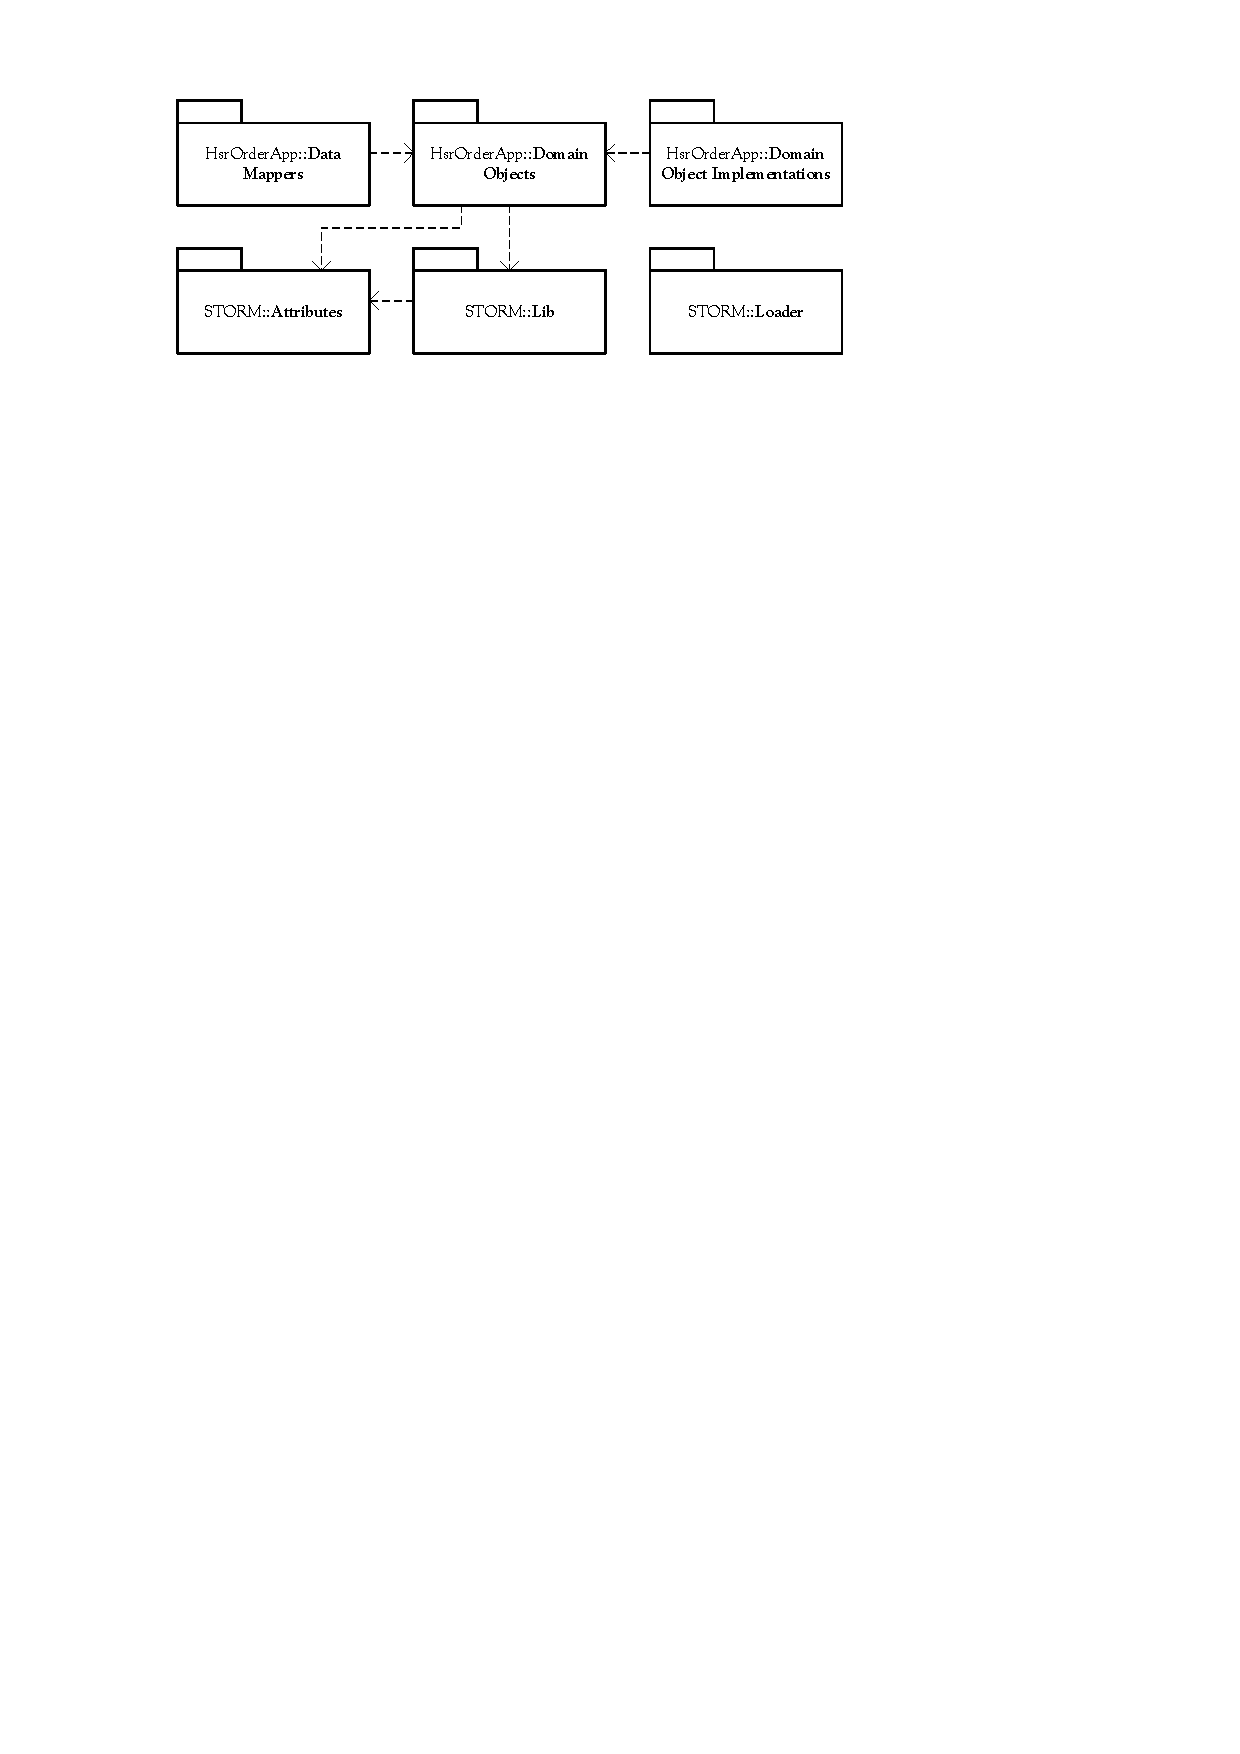
\includegraphics{./files/inc/figures/designPackages}
				\caption{\label{fig:designPackages} Software Packages}
			\end{center}
		\end{figure}
		
		The \verb~HsrOrderApp::Domain Objects~ package contains all abstract classes. These classes
		are needed to generate the mapping code. This is the starting point to write an application.
		The other two packages in \verb~HsrOrderApp::~ contain only generated code. This code
		is split into implementations of the domain objects and the mapping code for each domain
		object.
		
		The more important packages are \verb~STORM::~. The \verb~::Attribute~ package contains
		all custom attributes. This includes attributes which are used internally only by \textit{STORM} and 
		attributes which can be used to attribute abstract classes. All these attributes are listed in section 
		\ref{sec:attributes}. The package \verb~::Lib~ contains all generic classes which \textit{STORM}
		provides. At last, the \verb~::Loader~ package contains the \verb~AssemblyLoader~ and other classes
		related to CodeSmith.
		
		The \verb~STORM::Lib~ package is the core of the \textit{STORM} framework. Figure \ref{fig:designLibConcept}
		shows a conceptional model of this package. Some classes are generic and only used
		by the classes in the domain object. In the following sections, the different concepts
		are described. 
		
		\begin{sidewaysfigure}[htbp]
			\begin{center}
			\thispagestyle{plain}
				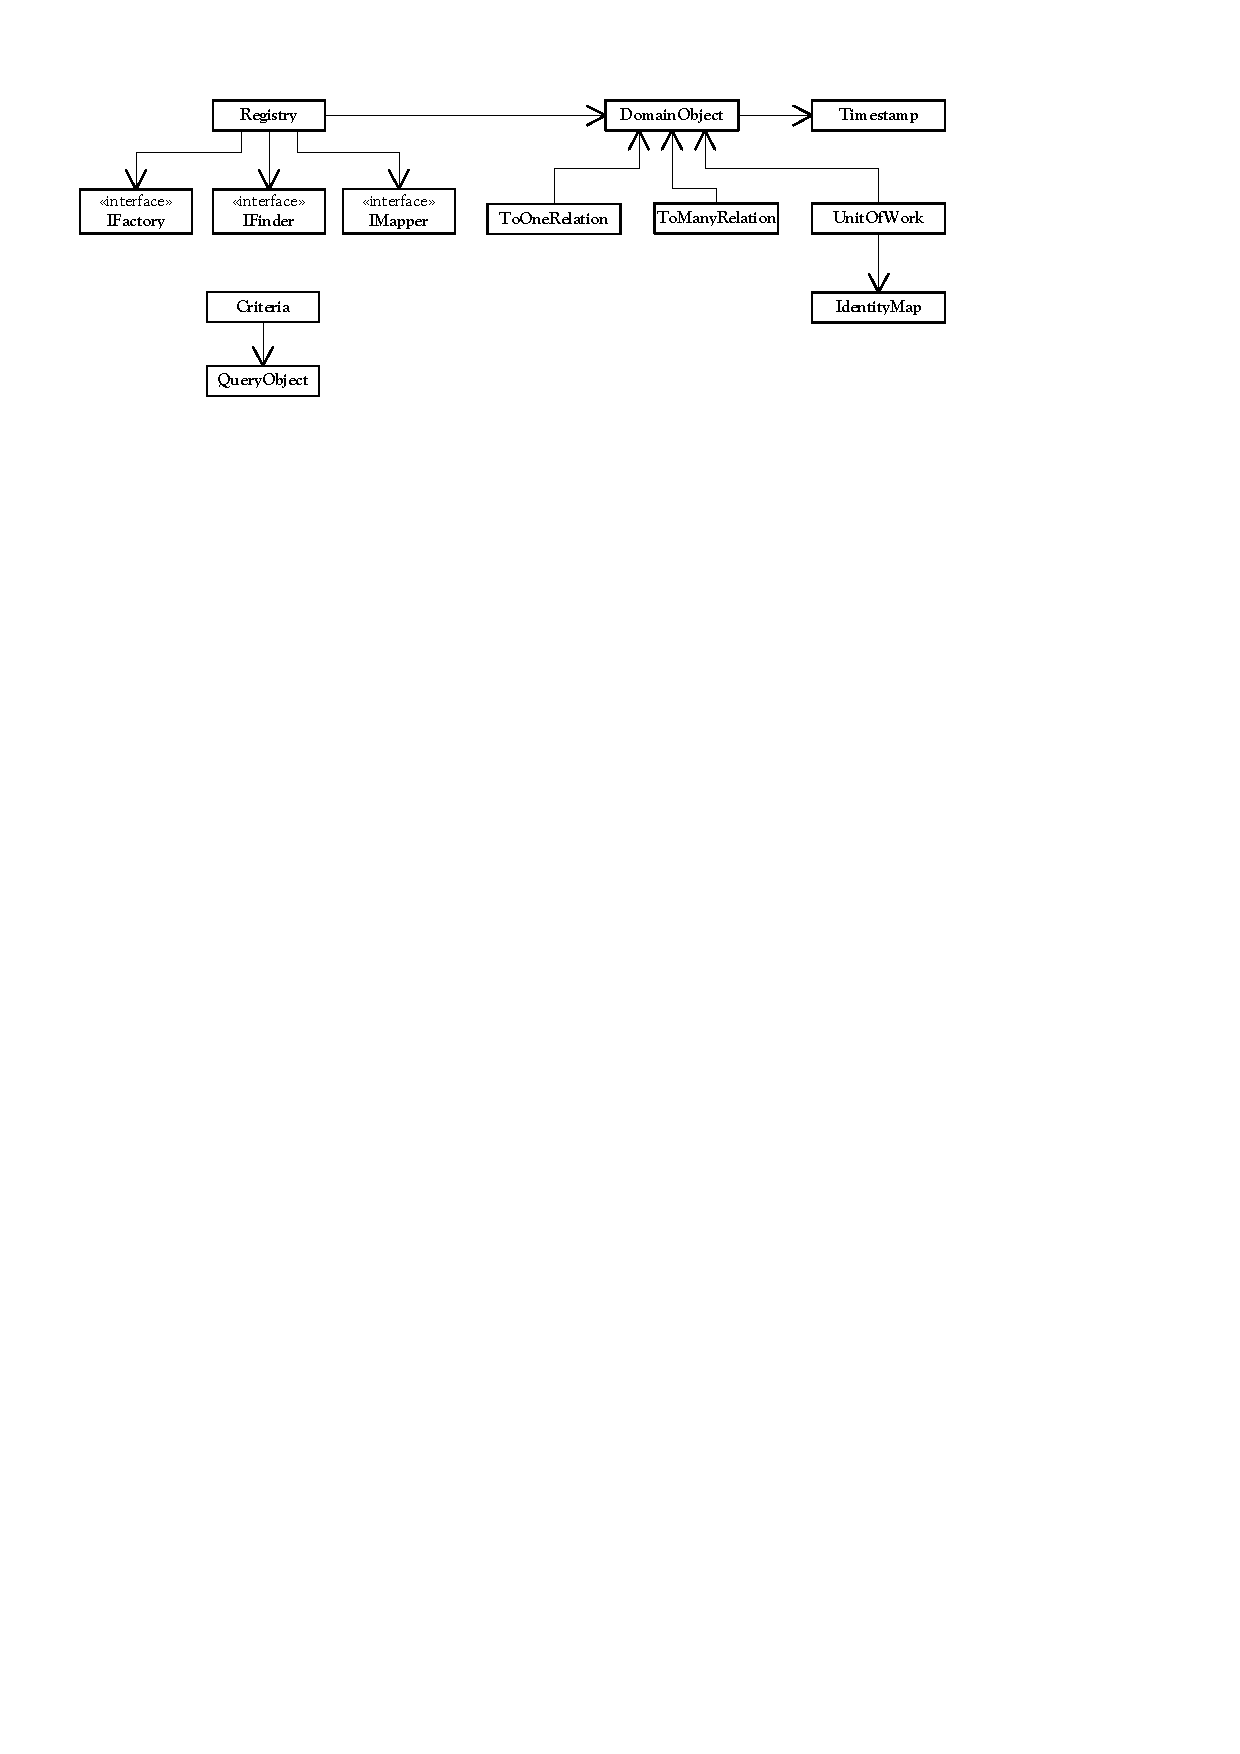
\includegraphics{./files/inc/figures/DesignLibConcept}
				\caption{\label{fig:designLibConcept} Conceptional Model of the STORM::Lib Package}
			\end{center}
		\end{sidewaysfigure}

				
	\section{Registry}
		As soon as an application starts, it must call the \verb~Registry~'s \verb~init()~ function.
		This function searches through all assemblies of the currently executed program and stores
		the type information of all domain object and mapper implementations in hashtables. These
		hashtables are used later to retrieve the appropriate implementation or mapper for a given
		type. Because we cannot know the type of implementations and mappers at design time, only
		interfaces are returned. This interfaces can be casted by the caller.
		The usage of the \verb~Registry~ is described in the following sections. Figure 
		\ref{fig:designRegistryAndInterfaces}	shows the registry class and the interfaces which are used
		in this context.
		
		\begin{figure}[htb]
			\begin{center}
				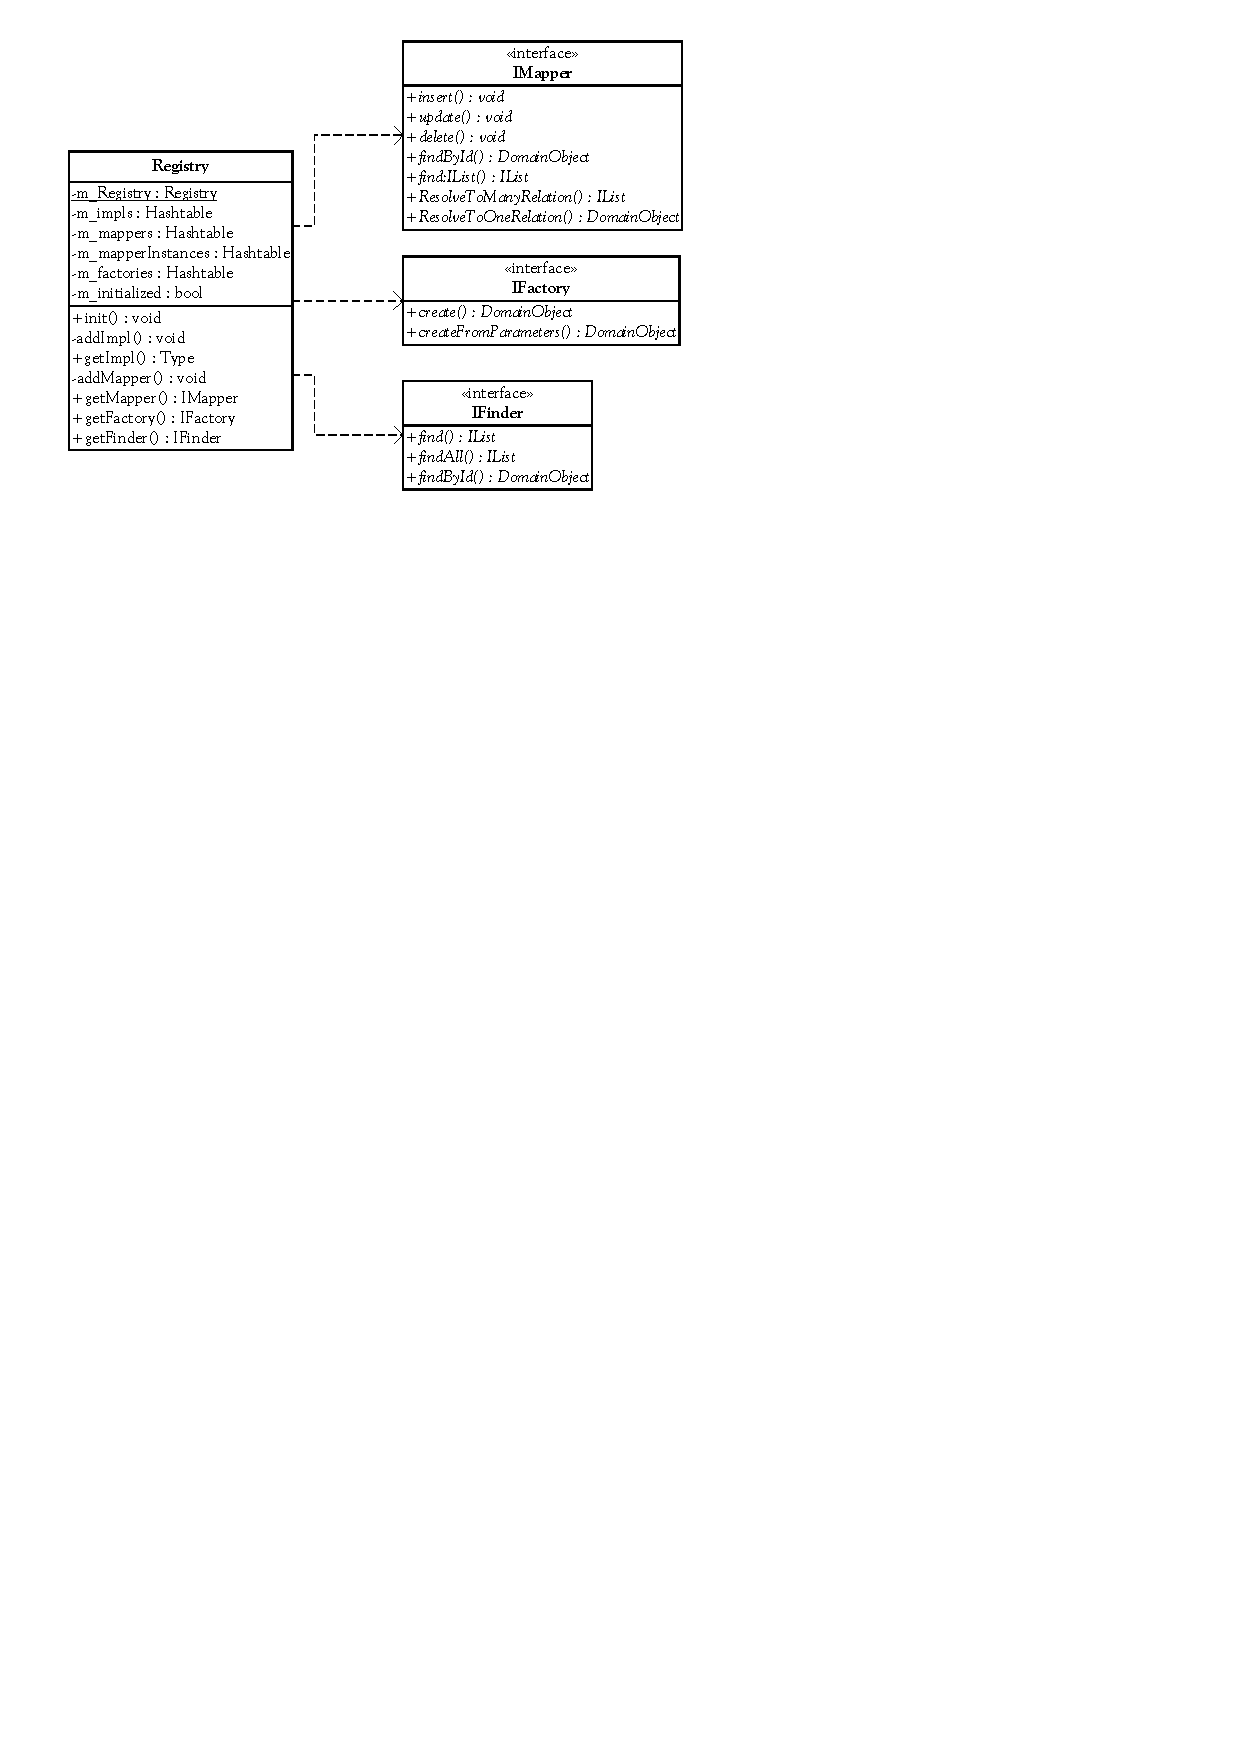
\includegraphics{./files/inc/figures/DesignRegistryAndInterfaces}
				\caption{\label{fig:designRegistryAndInterfaces} Registry and depending Interfaces}
			\end{center}
		\end{figure}
		
	\section{Unit of Work}
		A key concept in \textit{STORM} is the use of a \textit{Unit of Work} pattern. This pattern has
		already been described in section \ref{subsec:unitOfWork}. A UnitOfWork manages database
		connections and is responsible to execute database operations in the right order.
		
		Every time a new object is created, that object registers itself in the UnitOfWork as new.
		Similarly, if an object has been changed or deleted, that object registers itself as either
		dirty or removed.
		The UnitOfWork stores all this and executes the appropriate operations in the right order upon
		a commit request. If an object is transferred from the database, this object is registered as
		clean.
		
		Connections are handled through a \verb~Transaction~ object. Every time the UnitOfWork
		receives a commit request, it starts a new transaction. After all commands are executed,
		the transaction is closed. This is related to the locking mechanisms described in 
		section \ref{sec:lockingMechanisms}. Also the lifetime of a UnitOfWork has already been
		described in section \ref{sec:objectLifetime}.
		
	\section{Factory}
	\label{sec:Factory}
		As mentioned in chapter \ref{cha:designConsiderations}, it is important to avoid dependencies
		between generated and non-generated code. The solution is to use the \textit{Factory Method} pattern.
		In the case of \textit{STORM}, this means that whenever a new object is created, it must be 
		handled through the \verb~Registry~. This is somewhat more complicated but the most proper
		solution for it. For example, if a client wants to create a new \verb~Person~, it needs a
		constructor for it. If this constructor was declared in the abstract class, it would be
		of no use because abstract classes cannot be instantiated. And because of the dependency
		problem, a constructor in the domain object implementation cannot be called directly. But again, in order
		to create a new \verb~Person~, we need to call a constructor.
		
		The solution is to declare an internal class in the abstract domain object class and to parameterise
		it with the Factory attribute. This, for a \verb~Person~, would look like Listing
		\ref{lst:factoryClass}.
		
		\begin{lstlisting}[float=htb,language={[Sharp]C},caption=Defining a Factory Class,
		label=lst:factoryClass]
public abstract class Person : DomainObject
{
	[Factory]
	public abstract class PersonFactory
	{
		public abstract Person createPerson(
			[ParameterDef("PersonName")] string name,
			[ParameterDef("Password")] string password);
	}
}
		\end{lstlisting}
		
		Out of this declaration, a \verb~FactoryImpl~ and a static Property are generated 
		in the domain object implementation. When now a \verb~Person~ object should be created, the client can
		call the \verb~Registry~ for an appropriate FactoryImpl object. On this FactoryImpl object,
		the declared constructor can be called. Such a call would look like:
		\begin{Verbatim}
Person newPerson =
  ((Person.PersonFactory)Registry.Instance.getFactory(typeof(Person)))
  .createPerson("Jack", "password");
		\end{Verbatim}
		
		With this mechanism, there is no dependency between object which should not be. The drawback
		is that the usage is somewhat more complicated.
		
		Even if the Factory declaration in the abstract class is omitted, a FactoryImpl and a
		static Property will be generated in the domain object implementation.
		This is because the \verb~IFactory~ interface declares two methods to create an object. These
		methods can be called without declaring a custom Factory class in the abstract class. Furthermore,
		they are needed internally by \textit{STORM} to create objects which has been loaded from
		the database but do not exist as in-memory objects.
		
	\section{Finder Methods}
		\subsection{Self Defined}
			Another problem occurs with finder methods. Depending on the object in question, the
			finder methods will look differently. For example, a client wants to be able to call
			a method which looks like: 
			\begin{Verbatim}
public IList findByNameAndPassword(string name, string password){...}
			\end{Verbatim}
			This would return a list containing \verb~person~ objects which match the given name and password.
			The question is where to declare this methods.
			The solution is similar to the factory described in the last section. Finder methods
			can be declared in the abstract class as methods of a class attributed with the 
			\hyperlink{FinderAttribute}{Finder} attribute.
			An	example of such a declaration is given in Listing \ref{lst:finderClass}.
				
			\begin{lstlisting}[float=htb,language={[Sharp]C},caption=Defining a Finder Class,
			label=lst:finderClass]
public abstract class Person : DomainObject
{
	[Finder]
	public abstract class PersonFinder
	{
		public abstract IList findByName([ParameterDef("Name")] string name);
		public abstract IList findByNameAndPassword(
			[ParameterDef("Name")] string name,
			[ParameterDef("Password")] string password);
	}
}
			\end{lstlisting}
		
		Now, if a client wants to call a finder method, it asks the registry for an appropriate 
		finder implementation. On the returned object, the method can be called. Such a call would
		look like:
			
			\begin{Verbatim}
ArrayList foundPersons = new ArrayList();
foundPersons = ((Person.PersonFinder)Registry.Instance.getFinder(typeof(Person)))
               .findByName("Jack");
			\end{Verbatim}
			
			Because a finder method must be independent from a specific object (we do not want
			to create an object just to be able to call a find method), the implementation
			differs from the factory implementation. To be more precise, the code for
			a finder method must be in a appropriate mapper implementation, e.g. in the
			\verb~PersonMapper~. As we can see later, this is only true for generic finder methods.
			The reason is the following problem: A client cannot call
			a method which is defined in the abstract class and implemented in the mapper implementation.
			That is because a mapper implementation is not inherited from the abstract class
			(in contrast to the domain object implementations).
			Therefore, an implementation of the finder
			methods must persist in the domain object implementation such that a client is
			able to call it.
			
			The next consideration is how to call the generic finder method in the mapper implementation
			from within the domain object implementation. The solution is to use a 
			\textit{Query Object} pattern. With a query object, every custom defined finder method
			can be converted to an appropriate query object which then can be passed to 
			a generic finder method in the mapper implementation. Generic finder methods are described
			in \ref{subsec:genericFinder}.
			
			Figure \ref{fig:designFind} is a sequence diagram showing this finding scenario.
			
			\begin{figure}[htb]
				\begin{center}
					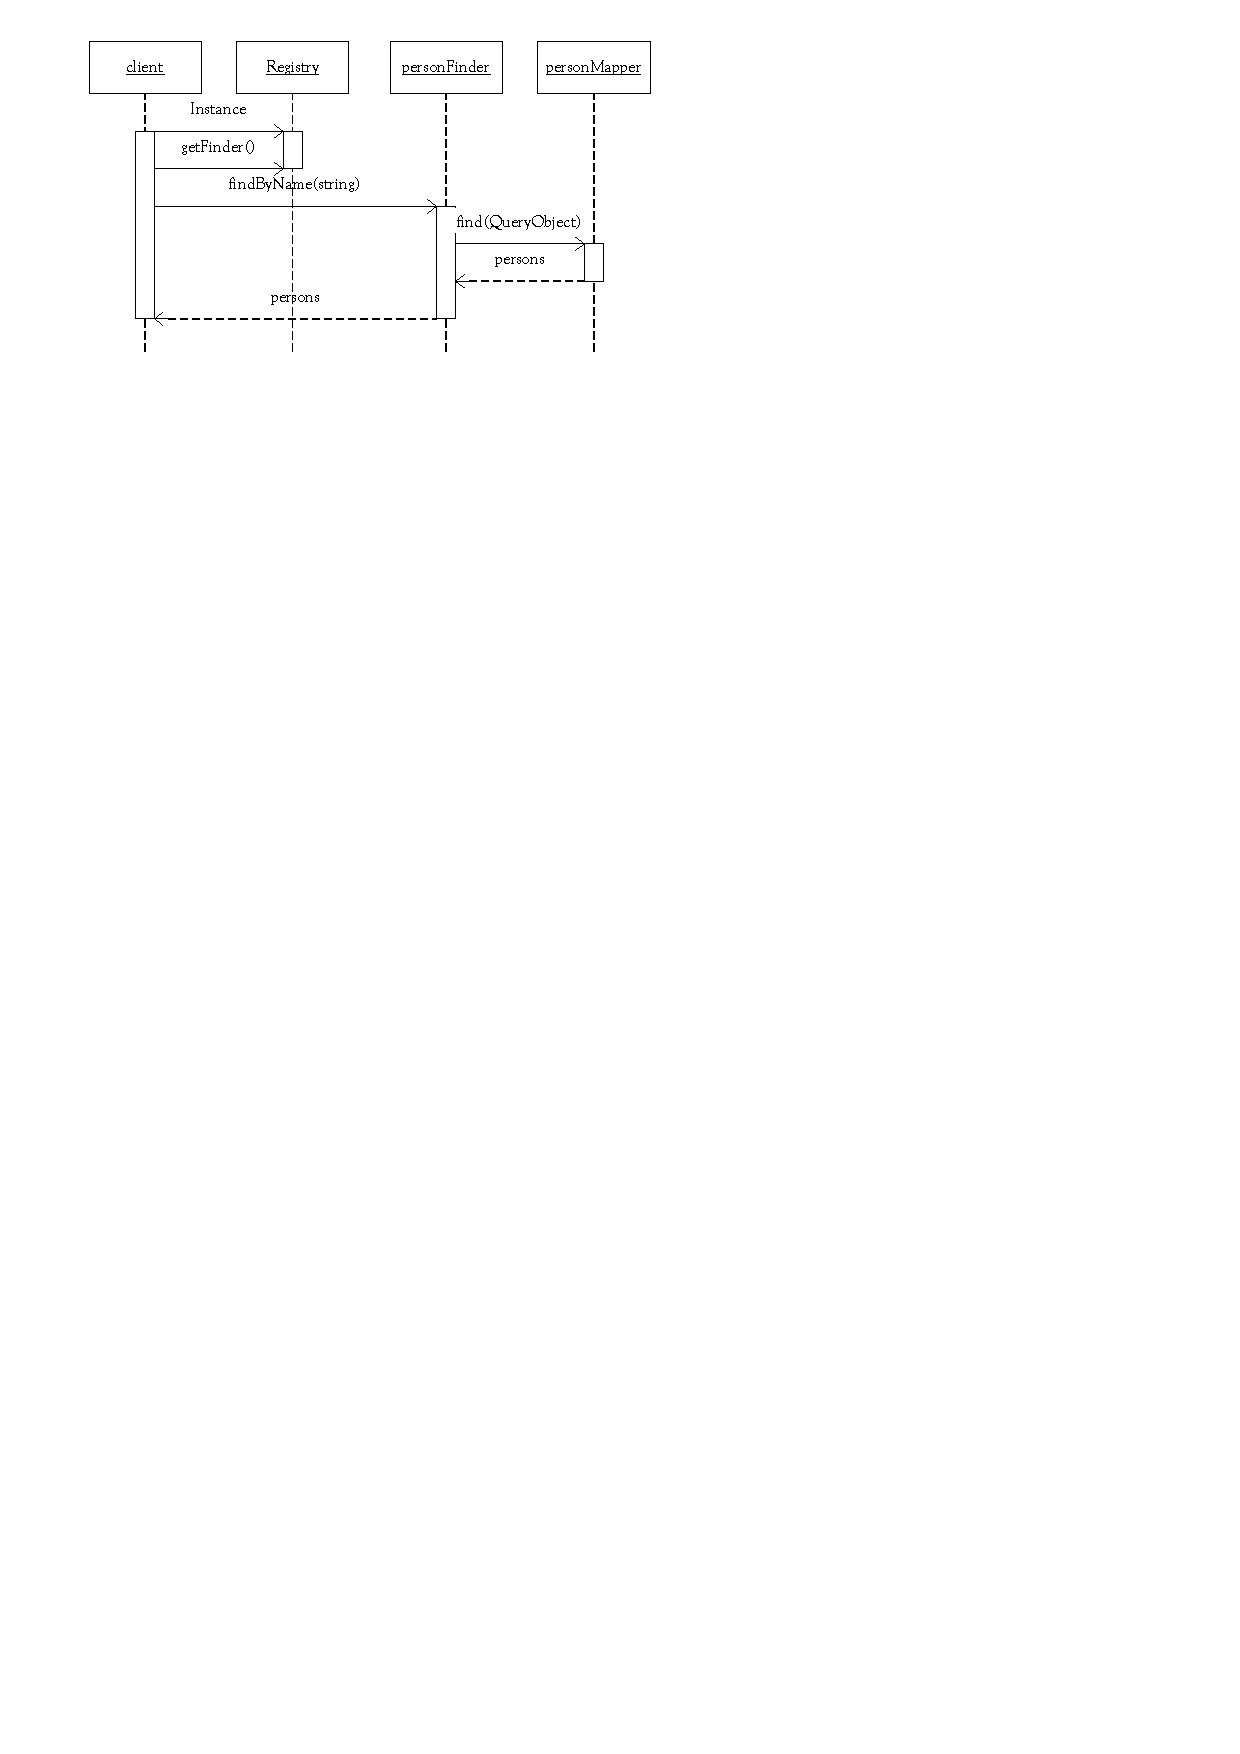
\includegraphics{./files/inc/figures/DesignFind}
					\caption{\label{fig:designFind}Finding objects with custom finder methods}
				\end{center}
			\end{figure}
			
		\subsection{Generic}
		\label{subsec:genericFinder}
			Because some finder methods are known and can apply to every type of object, not all finder methods must
			be self defined. Those methods which are generic have been made accessible through an interface (\verb~IFinder~).
			The implementation of these methods is in the mapper implementation class. 
			The following methods have been declared in the \verb~IFinder~ interface:
			\begin{Verbatim}
IList find(QueryObject qo);
IList findAll();
DomainObject findById(Key id);
			\end{Verbatim}
			
			The first method takes a \verb~queryObject~ as parameter. This object holds any number
			of \verb~criteria~ objects. If multiple \verb~criteria~ objects are added to a \verb~queryObject~, they
			are linked together with ``AND''. To stay with our person example, a call to find
			every person whose name is 'Jack' would look like:
			
			\begin{Verbatim}
QueryObject qo = new QueryObject();
qo.addCriteria(new Criteria(Criteria.Operator.Equal, "Name", "Jack"));

ArrayList foundPersons = new ArrayList();
foundPersons = Registry.Instance.getFinder(typeof(Person)).find(qo);
			\end{Verbatim}
			
			These makes it possible to form self defined find constructs through a \textit{Query Object}.
			The result is the same as to define a method in the abstract class but sometimes it is  more
			flexible to use. Figure \ref{fig:DesignQueryObjectAndCriteria} shows the 
			\verb~QueryObject~ class and its relation to \verb~Criteria~.
			
			The other two methods are self explaining and can be used accordingly.
			
			\begin{figure}[htb]
				\begin{center}
					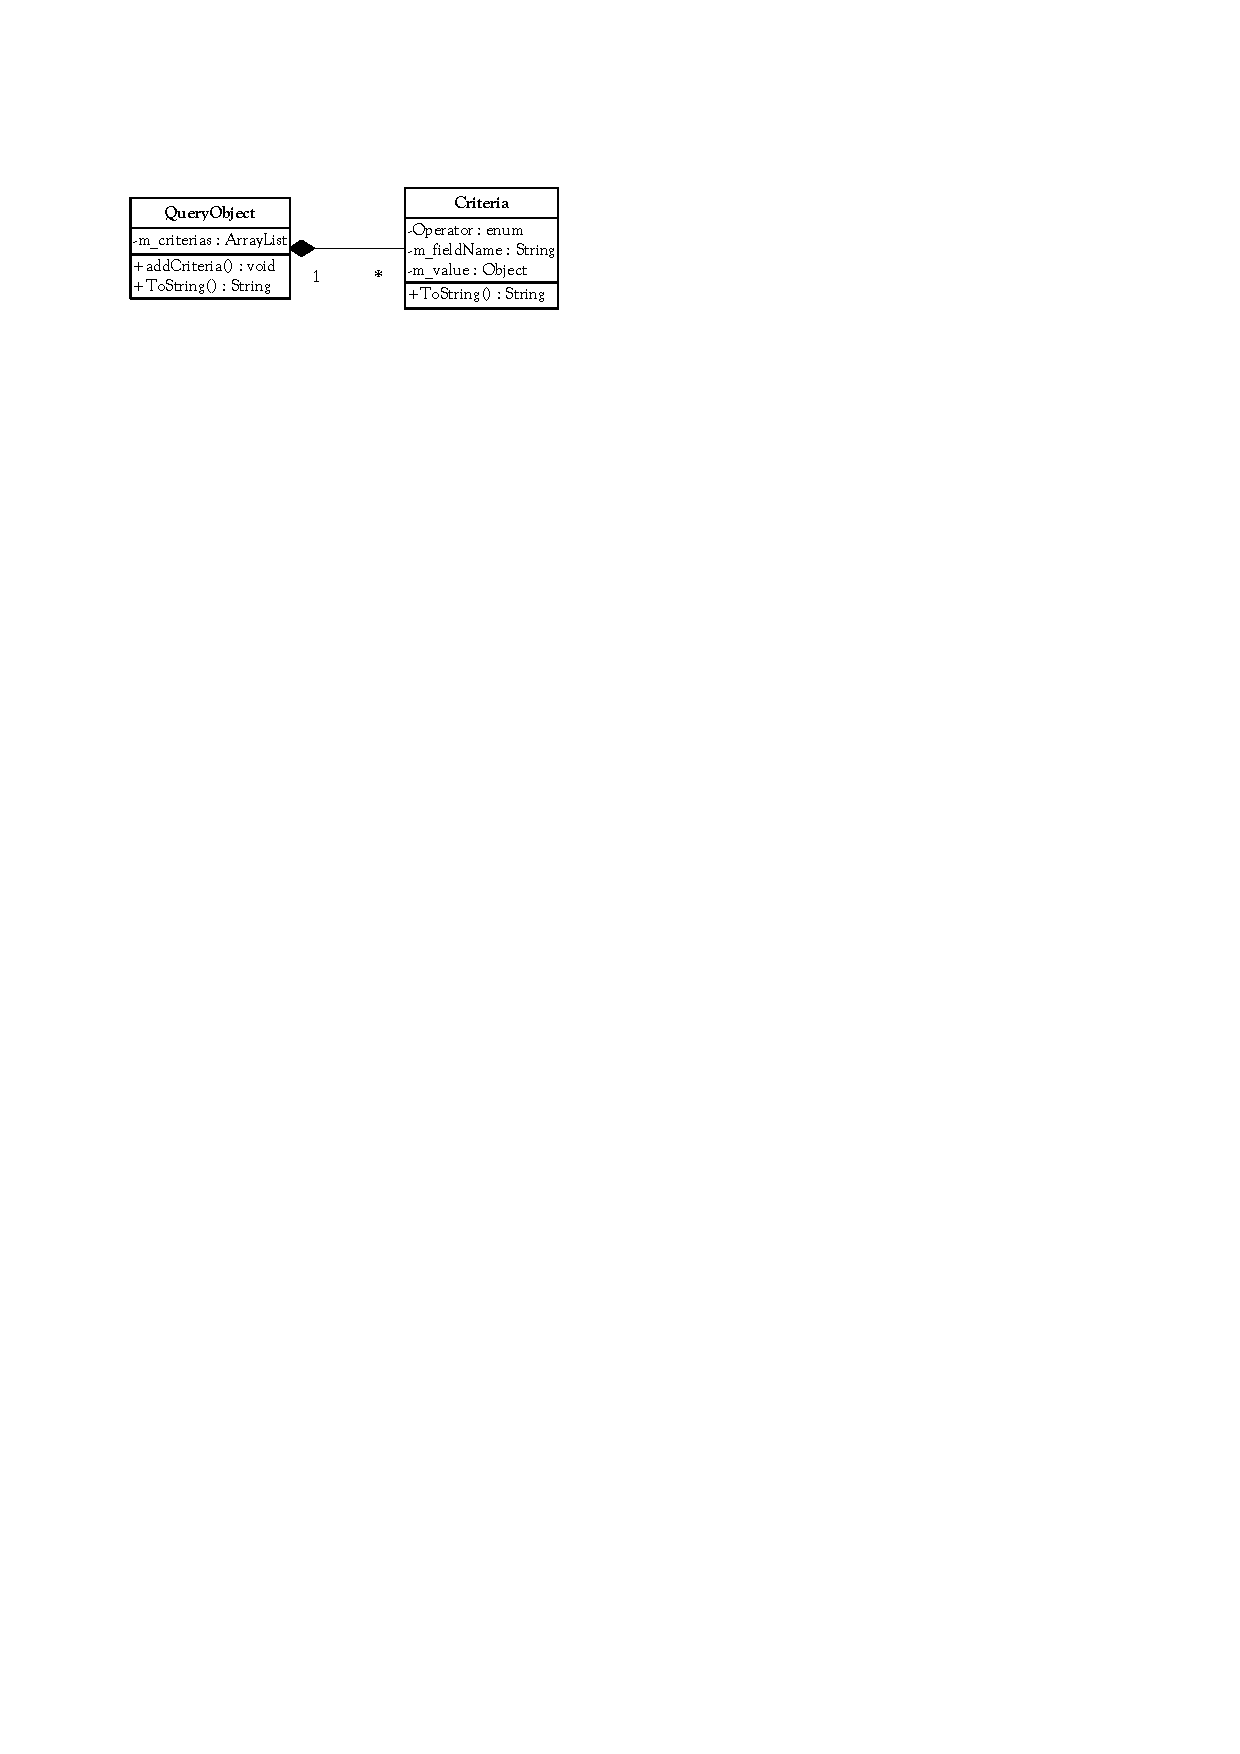
\includegraphics{./files/inc/figures/DesignQueryObjectAndCriteria}
					\caption{\label{fig:DesignQueryObjectAndCriteria}Relation between QueryObject and Criteria}
				\end{center}
			\end{figure}
			
	
	\section{Adder Methods}
		Adder methods are those which can be used to add related objects to the current object. For example,
		a \verb~person~ can have an adder method to add \verb~address~ objects which are related to
		the person (e.g. her/his addresses). This is different from creating and finding objects because an
		adder method must be called on the object itself, e.g. on a \verb~person~ object. This means,
		an object must be existing. Therefore, the only sensible place to have adder methods
		implemented is the domain object implementation.
		
		Adder methods are used in conjunction with \hyperlink{ToManyAttribute}{ToMany}
		relations. A code snippet from the abstract class \verb~Person~ is given in Listing
		\ref{lst:personAdder}. The example defines a ToMany relation and a belonging adder method.
		
		\begin{lstlisting}[float=htb,language={[Sharp]C},caption=Defining an Adder Method,
			label=lst:personAdder]
[ToMany(typeof(Order), "Person")]
public abstract IList Orders {get;}

[Adder("Orders", "Person")]
public abstract void addOrder(Order o);
		\end{lstlisting}
		
		The code for all adder methods is generated into the domain object implementation.
		For example, the resulting code for the adder method shown in \ref{lst:personAdder}
		looks like (exception handling is omitted):
		
		\begin{lstlisting}[float=htb,language={[Sharp]C},caption=Defining an Adder Method,
			label=lst:personAdderImpl]
public override void addOrder(Order o)
{
	if(o != null)
	{
		o.Person = this;
		m_Orders.Add(o);
	}
}
	\end{lstlisting}
	
	m\_Orders is an object of type ToManyRelation which holds all related objects. Adder methods
	could be generated automatically, but again, if they were, it would not possible to call
	those methods from a client. o.Person is the back reference from an order to a person.
	
	%----------
	\section{Data Flow}
		This section is about the work flow of \textit{STORM}. It covers and explains
		the most important flow scenarios. These are creating new objects, deleting objects and lazy load.
		
		\subsection{Create New Object}
			A new object is represented in an application with a new instance of a class. This
			instance is registered within the \textit{Unit of Work} as new. Whenever the \textit{Unit of Work} 
			receives a commit, this new class needs to be written to the database. For this, a new
			transaction is created after the commit is received. A transaction represents a database connection
			for a certain, limited time. In this case, a transaction is created at the beginning of the
			commit method and is closed at its end. For the time of this transaction, the database
			is exclusively locked. To actually write the new created object to the
			database, the specific mapper's \verb~insert()~ method is called. This method 
			writes the object to the database. The whole process is illustrated in Figure
			\ref{fig:designNewObject}.
			
			\begin{sidewaysfigure}[htb]
				\begin{center}
				\thispagestyle{plain}
					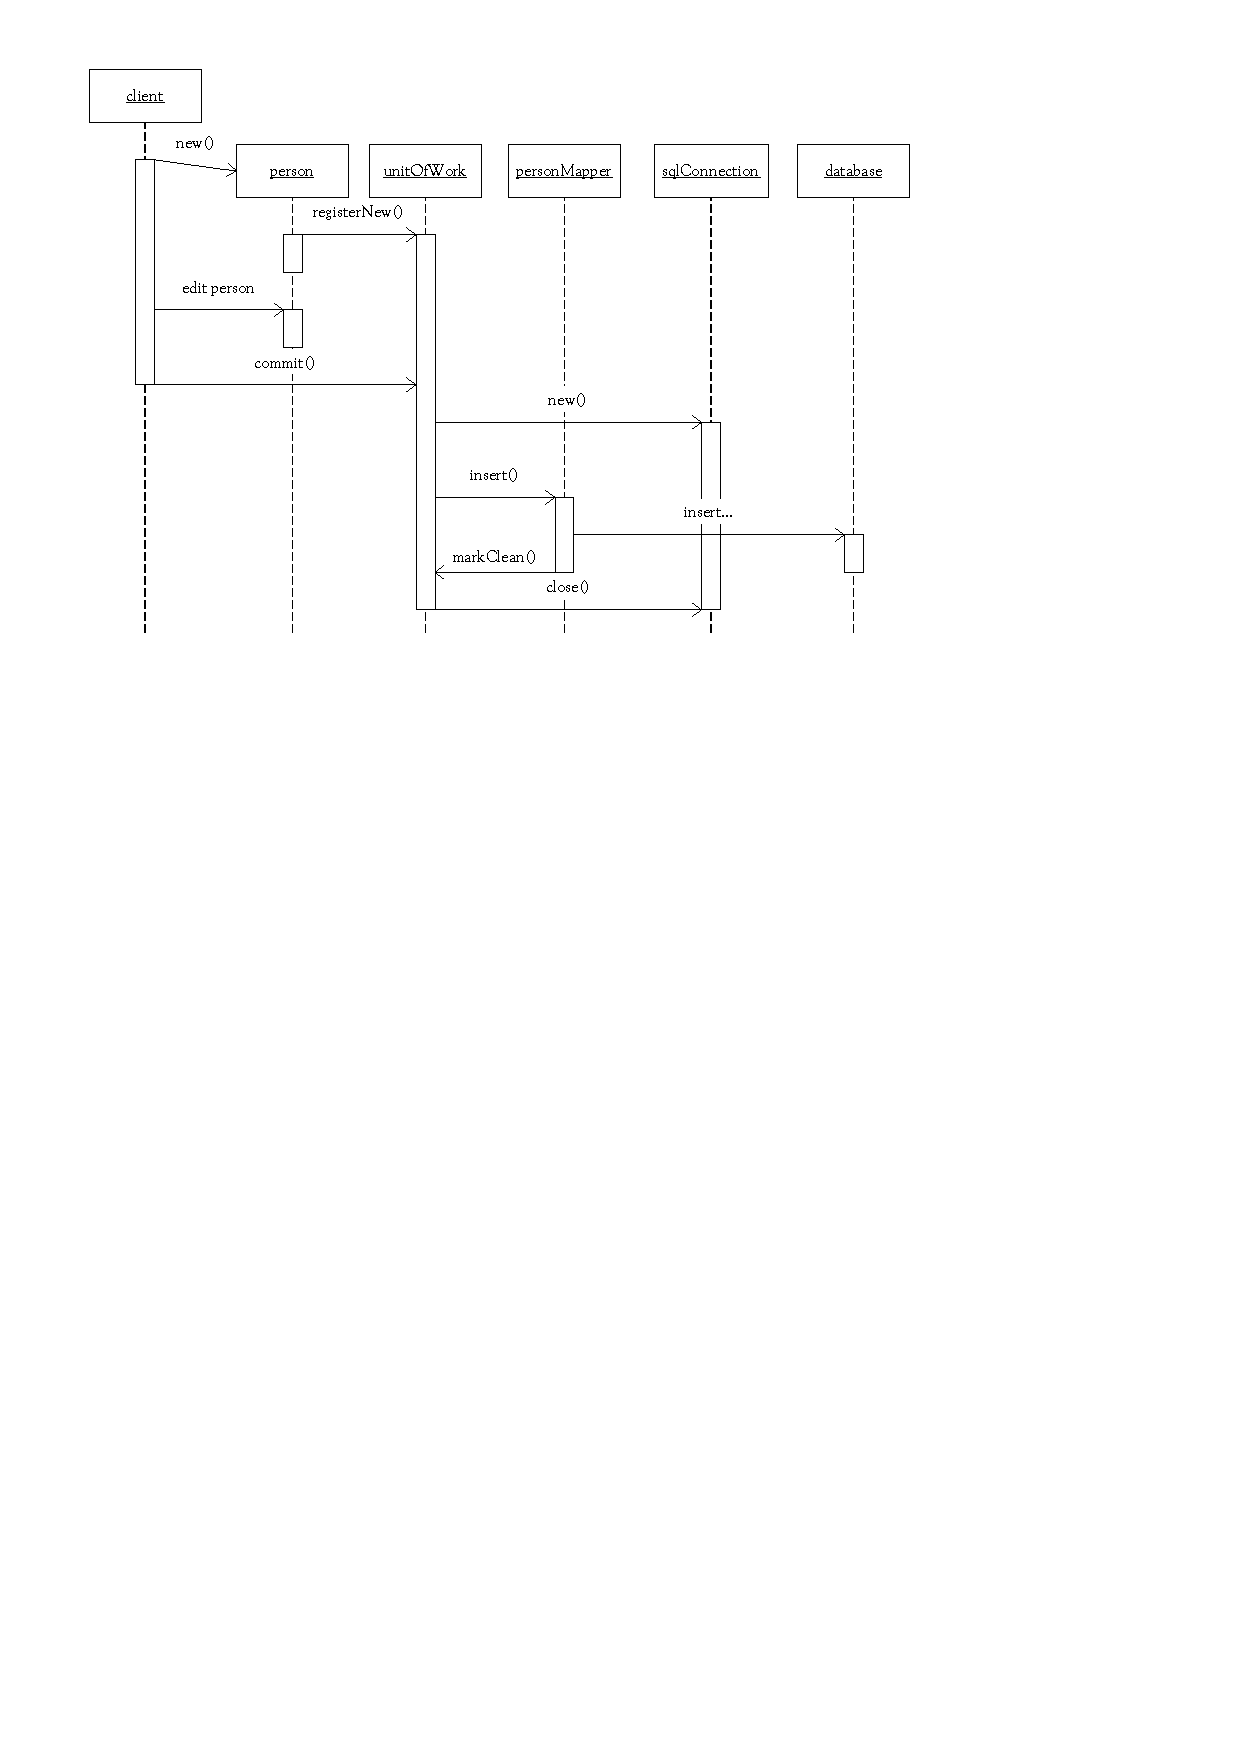
\includegraphics{./files/inc/figures/DesignNewObject}
					\caption{\label{fig:designNewObject} Creating a new Object}
				\end{center}
			\end{sidewaysfigure}

		\subsection{Lazy Load}
		\label{subsec:LazyLoad}
			Our object/relational mapper not only handles the mapping between classes and tables etc., it
			provides a mechanism to enhance performance. Vital to every application which transfers
			object over a network is to limit the number of remote calls. \textit{Lazy Load} provides
			a mechanism to handle this need. When talking about \textit{Lazy Load}, a few decisions need to be
			made before implementing a concrete solution. The most important concerns object lifetime. There are
			3 main ways which are as follows:
			\begin{enumerate}
				\item Whenever an object needs to be loaded, it will be fully loaded from the database,
							regardless of the fact if it had been already loaded before.
				\item	Before loading an object from the database, a class (see Identity Map \ref{subsec:identityMap}) which holds
							already transfered objects in a map is called to check if the object had been transferred before. 
							If so, the desired object is loaded	directly from this map instead of transferring it again. This
							sounds like a good alternative to the first mechanism but has the disadvantage of possible consistency
							errors. This leads to conflict resolution strategies which can be quite challenging to solve.
				\item	The third possibility is close to the second one except that an object's version field is compared
							with the version field on the database to check if the object is still up to date. If those versions
							match, the object from the map is loaded, otherwise the object will be reloaded from the
							database.
			\end{enumerate}
			The first strategy is the most simple to implement. It does not need an \textit{Identity Map} nor 
			\textit{Lazy Load}. Event though, it is not the most performant solution because objects are transferred
			more often. The second strategy would be, depending on the application though, more performant but much
			more complicated to implement. Additionally, it is not a good solution for code generation because
			conflict resolution strategies are very specific and can therefore not be generated automatically.
			For these reasons, we use the third strategy which should result in a good performance and a secure
			way to update objects. The process is illustrated in Figure \ref{fig:designLazyLoad}. It shows
			a find operation where all addresses for a person are searched.

			\begin{sidewaysfigure}[p]
				\begin{center}
					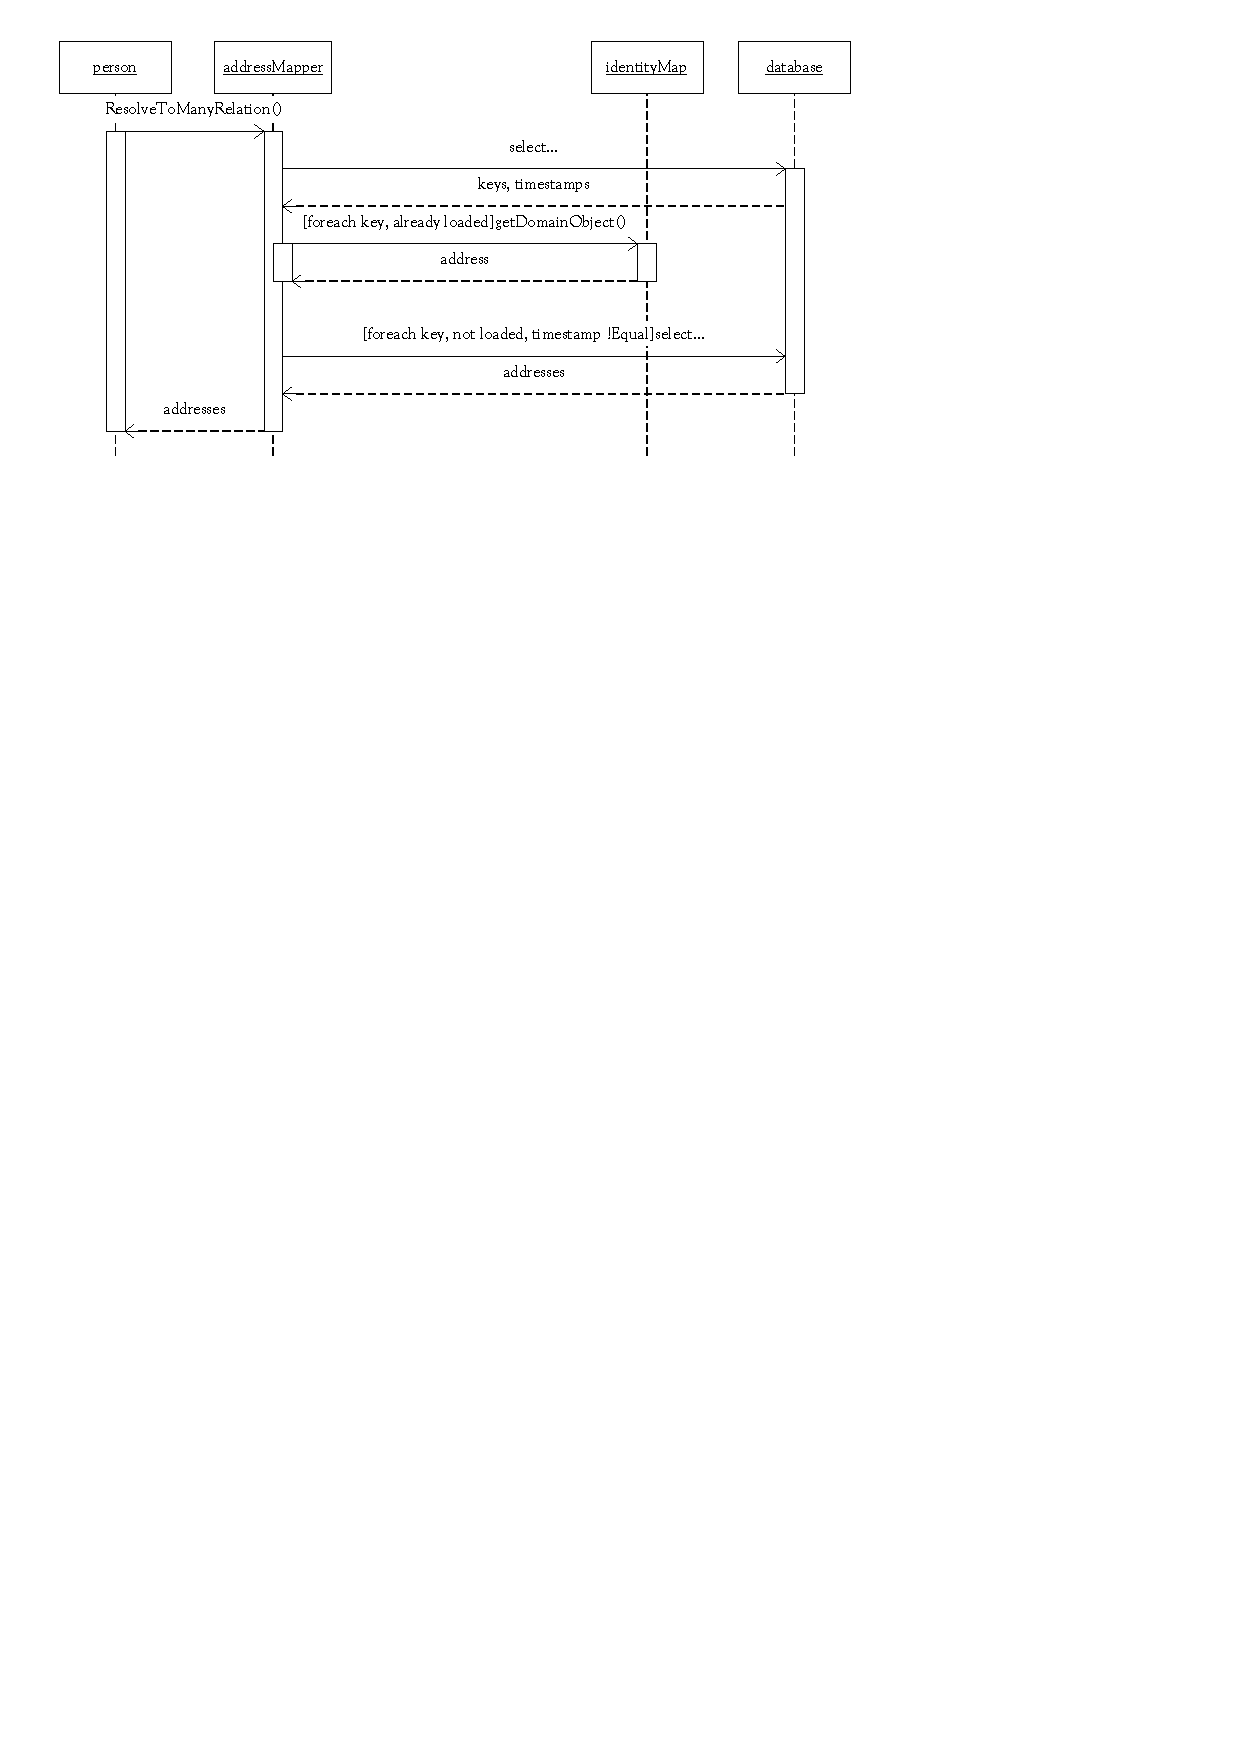
\includegraphics{./files/inc/figures/DesignLazyLoad}
					\caption{\label{fig:designLazyLoad} Lazy Load mechanism}
				\end{center}
			\end{sidewaysfigure}
			
		\subsection{Delete Object}
			Another scenario originates when an object (e.g. a Person) is deleted. It is not
			possible to just delete the person on the database because a person can have
			relations like addresses which has to be deleted first.
			In our example, this means to call the delete function on each address. The Address 
			will be marked as removed and registers itself in the UnitOfWork to be removed.
			After all addresses have been processed, the person
			itself can be registered to be removed. Because the \textit{Unit of Work} remembers
			the correct order, all addresses will be removed before the person is removed.
			Figure \ref{fig:designDelete} shows this procedure. \textit{Lazy Load}
			is also used to make sure that all objects are up to date but it is omitted in the
			sequence diagram.
						
			\begin{sidewaysfigure}[p]
				\begin{center}
					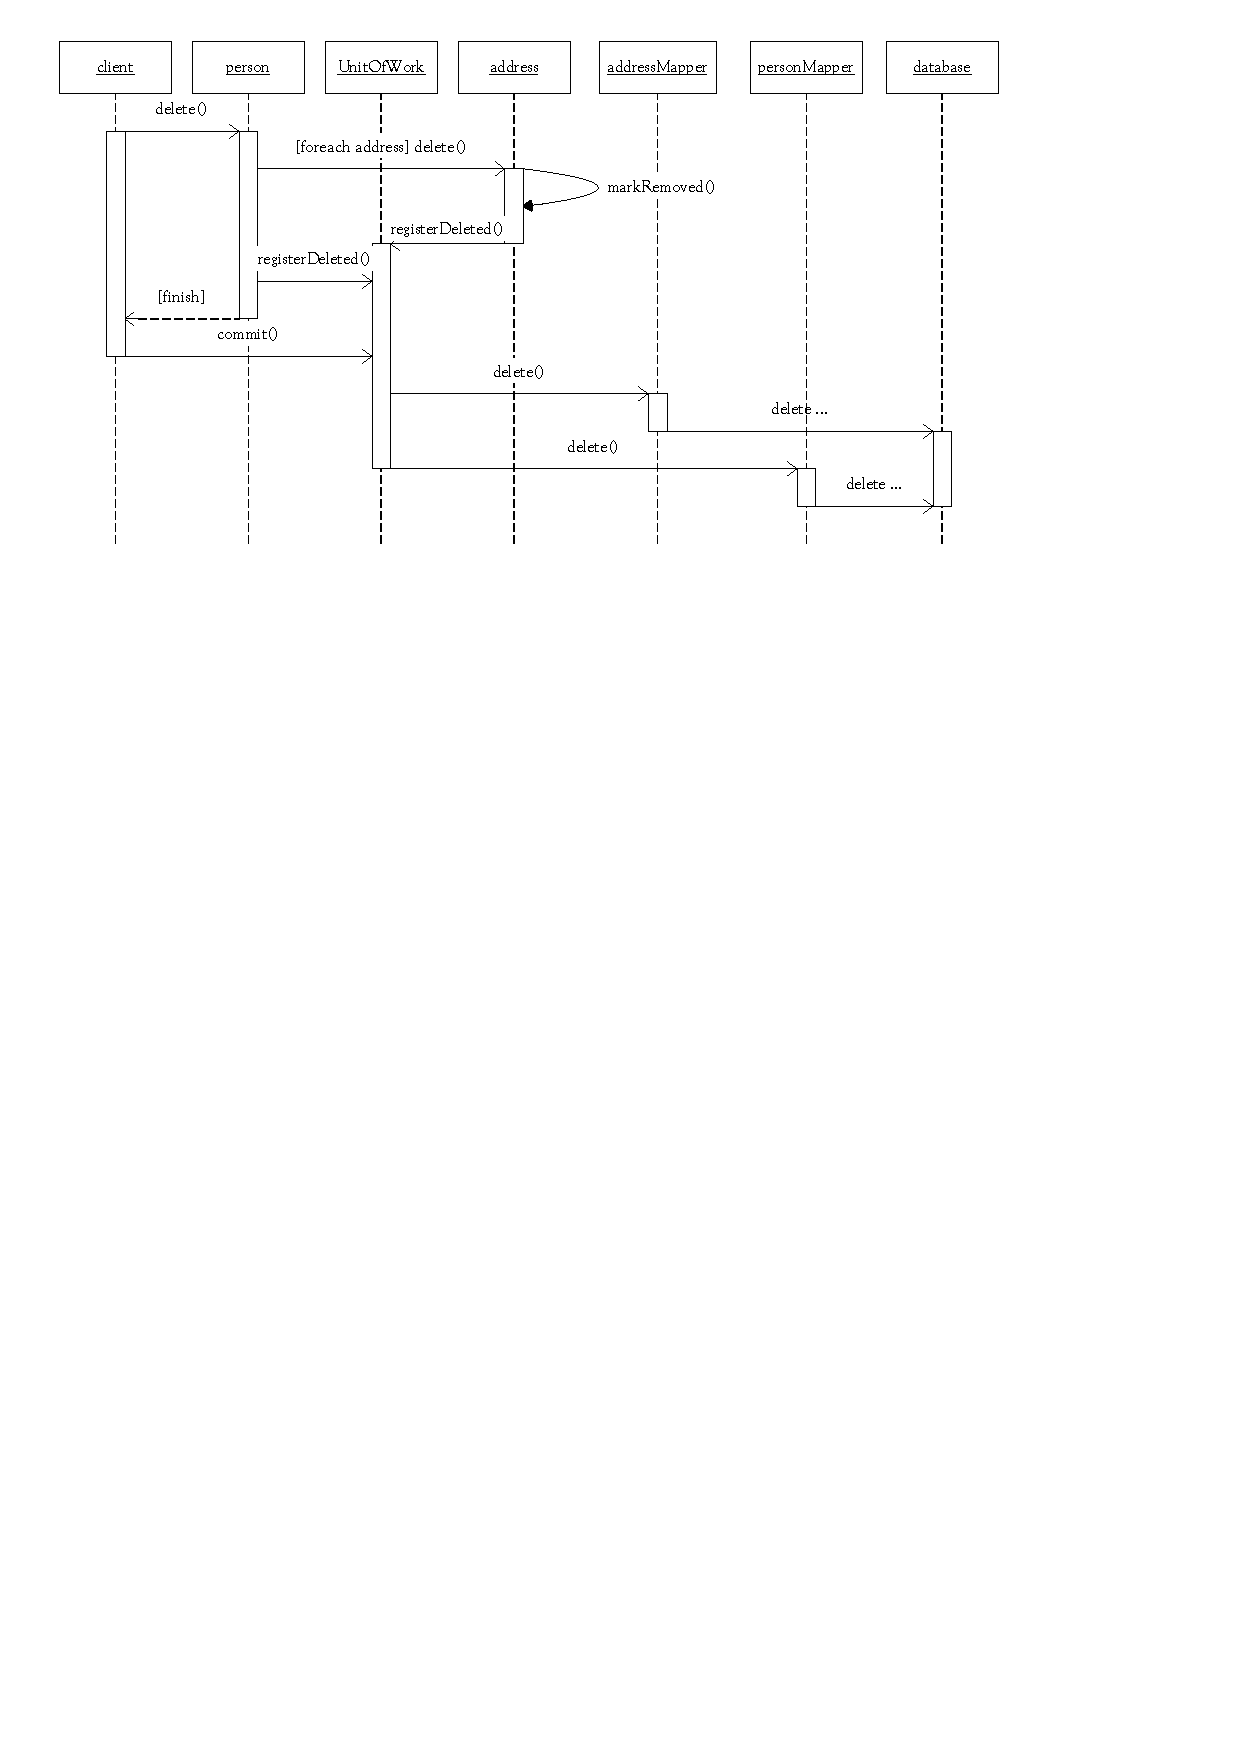
\includegraphics{./files/inc/figures/DesignDelete}
					\caption{\label{fig:designDelete} Delete an Object}
				\end{center}
			\end{sidewaysfigure}
			
	%----------
	\section{Attributes}
	\label{sec:attributes}
		Here is a list of all custom attributes which \textit{STORM} defines:
		
		\LTXtable{\linewidth}{./files/inc/tables/designAttributes}
		
		The following description list describes each attribute. This is only a short description
		meant as an overview.
		Parameter description is omitted.
		\begin{description}
			\item[Adder]
				Defines a method to add any objects to the current object. For example, it can be used
				to add an \verb~Address~ object to a \verb~Person~ object. This attribute is usually used
				for a \hyperlink{ToManyAttribute}{ToMany} relation. It is needed
				because an adder could not be called it it was generated automatically in the domain
				object implementation.
			\item[Column]
			\hypertarget{ColumnAttribute}{}
				Defines the mapping between a member variable and a column in the database. It is used for
				properties only. Out of these properties, the corresponding member variables are generated.
			\item[DomainObjectImpl]
			\hypertarget{DomainObjectImplAttribute}{}
				This is an internal only attribute. It must not be declared in an abstract class. Instead, it
				is automatically declared in the generated code and is used by the registry to know 
				which generated classes are to be treated as a domain object implementation and 
				should therefore be registered in the registry.
			\item[Factory]
			\hypertarget{FactoryAttribute}{}
				This attribute is used to specify the factory. It is used to attribute an abstract class declaration.
				Within this class, create methods can be specified. Out of this specification, constructors
				are generated which can be called from within a user written client program. A class specified with
				the Factory attribute must be enclosed by the main abstract class.
			\item[Finder]
			\hypertarget{FinderAttribute}{}
				Like the \hyperlink{FactoryAttribute}{Factory} attribute,
				this is an attribute which is used for an abstract class. Within this class, abstract methods
				can be declared. Out of these declaration, custom defined finder methods are generated.
			\item[GenerateCode]
				This attribute is used for every user defined, abstract class to indicate that
				code for this class should be generated. If omitted, the class will be completely
				ignored by \textit{STORM}.
			\item[MapperImpl]
				This is an internal only attribute. It must not be declared in an abstract class. Instead, it
				is automatically declared in the generated code and is used by the registry to know 
				which generated classes are to be treated as a mapper implementation and 
				should therefore be registered in the registry.
			\item[ParameterDef]
				This attribute is used in within the abstract \hyperlink{FactoryAttribute}{Factory} and
				\hyperlink{FinderAttribute}{Finder} classes. They define the mapping between
				parameters and the corresponding properties.
			\item[PrimaryKey]
			\hypertarget{PrimaryKeyAttribute}{}
				Declares that the primary key in the database is represented by this property. This attribute
				must always be used in conjunction with a \hyperlink{ColumnAttribute}{Column} attribute.
			\item[Table]
			\hypertarget{TableAttribute}{}
				This attribute maps the whole class to a table in the database. At this time, one class
				can only map to exactly one table. Additionally, this attribute declares if the
				\hyperlink{PrimaryKeyAttribute}{PrimaryKey} is a surrogate key or a compound key.
			\item[ToMany]
			\hypertarget{ToManyAttribute}{}
				Declares a relation to a collection of other objects. This maps a 1:n relation in the
				database to in-memory objects.
			\item[ToOne]
			\hypertarget{ToOneAttribute}{}
				Declares a relation to another object. This maps a 1:1 relation in the database to in-memory
				objects. It must be used to specify the back link to a \hyperlink{ToManyAttribute}{ToMany} relation.
				For example, if a \verb~Person~ specifies a \hyperlink{ToManyAttribute}{ToMany} relation to
				\verb~Address~, \verb~Address~ must declare a ToOne relation back to \verb~Person~.
				This attribute is always used in conjunction with a \hyperlink{ColumnAttribute}{Column} attribute.
			\item[VersionField]
				Specifies a version field in the database. This field is a auto-generated field of the data type
				\verb~timestamp~ and is used to check if the in-memory object is in sync with the database object.
		\end{description}
		
%\chapter{Creating an Application}
\label{cha:createApplication}

	\section{Introduction}
		The previous chapters were all about \textit{STORM}. This chapter should give
		you an overview of \emph{how to use} it. Even though it would be possible
		to create a new application in a relatively short time, we stay with our 
		order application example. This is not meant as a step by step guidance but
		as a ``not so short introduction to create an application with \textit{STORM}''.
		Some parts in this chapter have already been mentioned. They
		are repeated to put them in the context of creating a new application.
	
	\section{Starting a Design}
		In the case of the order application, the database design was already existing.
		Therefore, this has been taken as starting point. Usually, the starting
		point would be a domain model but it makes not much of a difference. The
		database design is shown in Figure \ref{fig:dbDesign}. The corresponding
		conceptional domain model is shown in Figure \ref{fig:designConceptModel}.
		The domain model looks essentially the same as the database model.
		This is because every domain object will be mapped to a table in
		the database. The design of an application is always the starting point
		and should be done carefully.
		
		Our order application is not very difficult to explain. It contains
		persons with addresses. One person can have multiple addresses. But an
		address in turn belongs always to only one person. Furthermore, a person
		can have multiple orders. An order contains order details which describe
		the order and its details like price and quantity. A product then
		is related to an order detail.
			
		\begin{figure}[htb]
			\begin{center}
				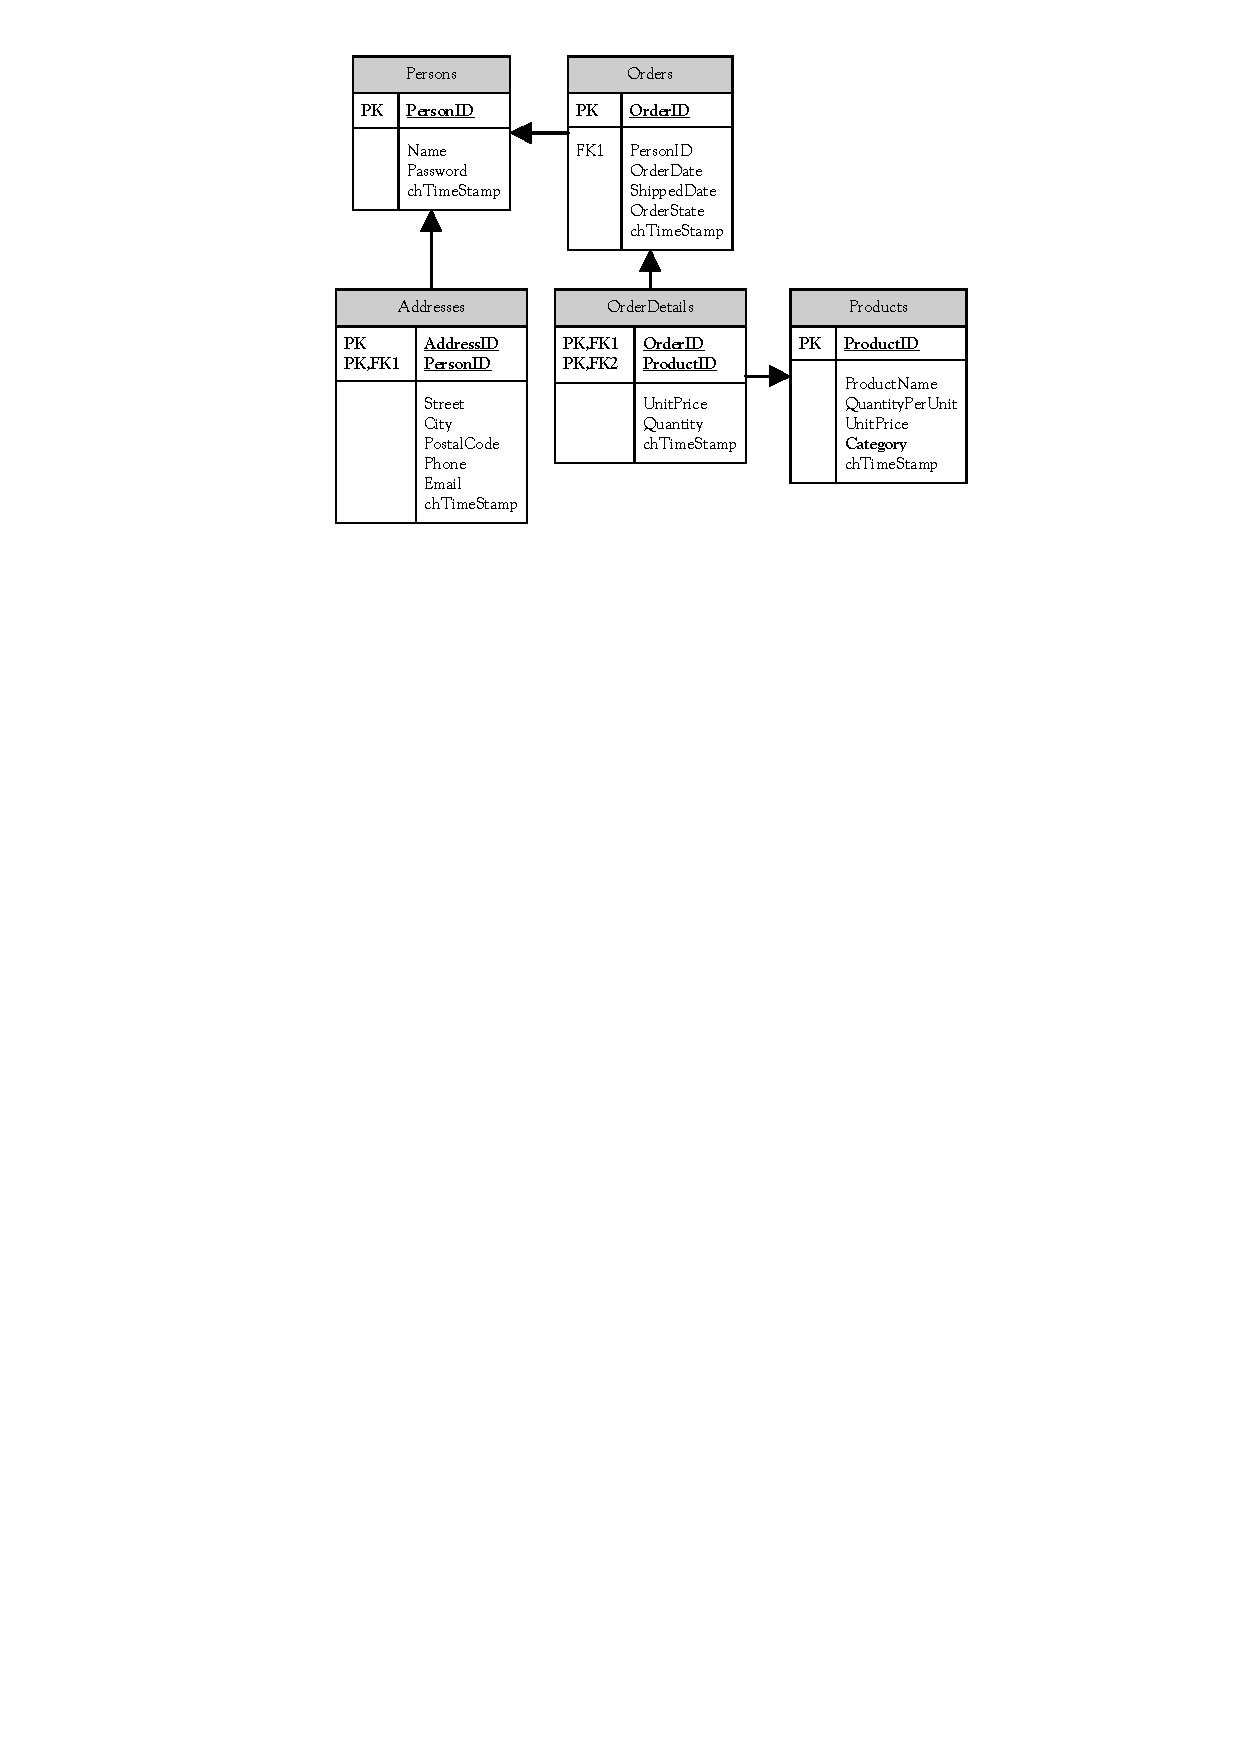
\includegraphics{./files/inc/figures/DbDesign}
				\caption{\label{fig:dbDesign}Database Design}
			\end{center}
		\end{figure}

		\begin{figure}[htb]
			\begin{center}
				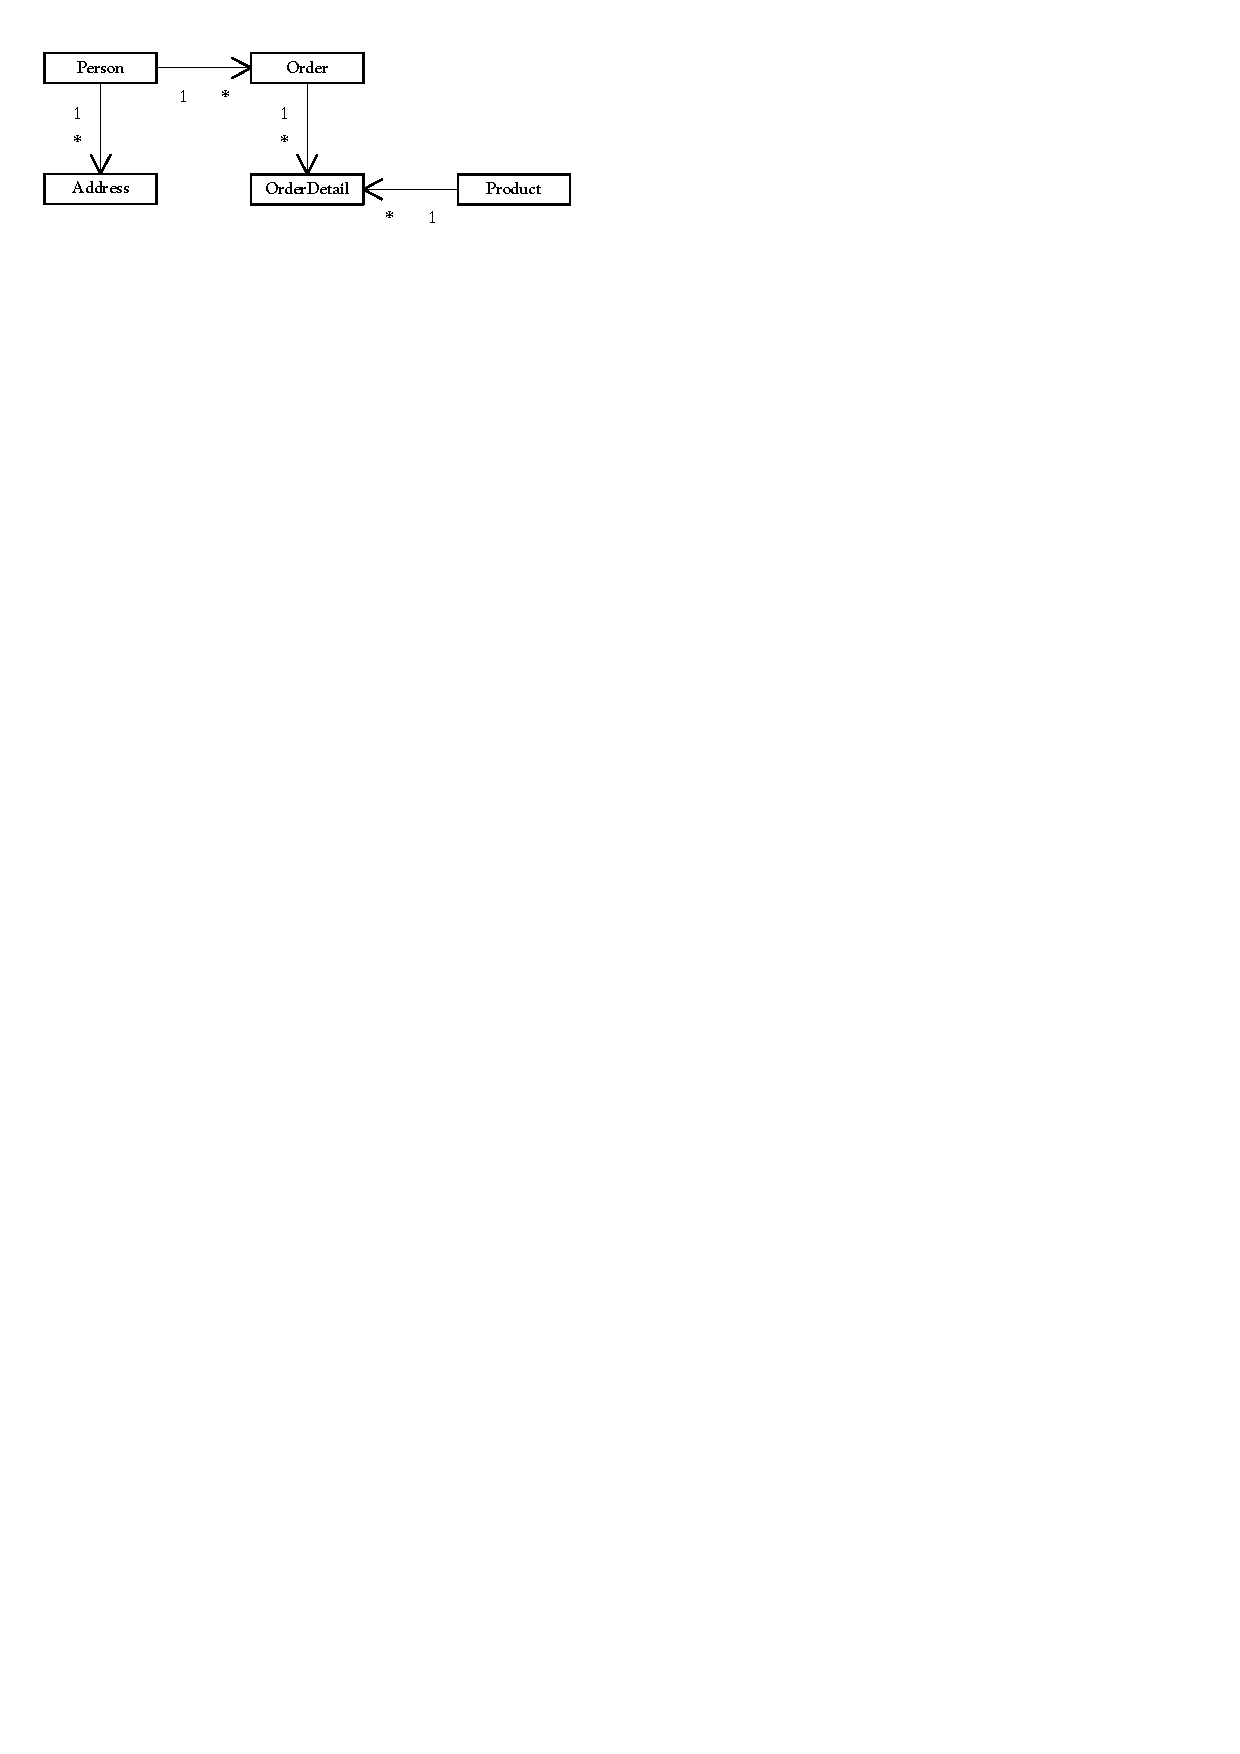
\includegraphics{./files/inc/figures/DesignConceptModel}
				\caption{\label{fig:designConceptModel}Conceptional Domain Model}
			\end{center}
		\end{figure}
		
	\section{Preparation}
		In order to work with \textit{STORM}, some preliminary work needs to be done.
		Namely that is to make the ImplGen and MapperGen templates available for the current
		project. This means, they must exist on the file system. Where to put them is
		the decision of the developer. The templates can be references by providing
		the full path. We decided to place the templates in a folder in the current project.
		The next step is to add a reference to the	new project. This reference must point to 
		the \textit{STORM} dll file. And last, CodeSmith \footnote{\url{http://www.ericjsmith.net/codesmith/}}
		must be installed. Thats it.
	
	\section{Writing abstract Classes}
		When all the design and preparation has been finished, it is time for \textit{STORM} to
		come into play. The first step is to write an abstract classes for each class of the
		domain model. In our case this means to write an abstract class for \verb~Person~,
		\verb~Address~, \verb~Order~, \verb~OrderDetail~ and \verb~Product~. It is very
		important to write these classes carefully. Listing \ref{lst:abstractOrderDetail}
		shows the abstract class \verb~OrderDetail~. 
		
		\begin{lstlisting}[language={[Sharp]C},caption=Defining OrderDetail as abstract class.,
		label=lst:abstractOrderDetail]
[Table("Orders", true),
VersionField("chTimestamp"),
GenerateCode]
public abstract class Order : DomainObject
{
	[Factory]
	public abstract class OrderFactory
	{
		public abstract Order createOrder(
			[ParameterDef("Person")] Person person,
			[ParameterDef("OrderDate")] DateTime orderDate,
			[ParameterDef("ShippedDate")] DateTime shippedDate,
			[ParameterDef("OrderState")] String orderState);
	}

	[Finder]
	public abstract class OrderFinder
	{
		public abstract IList findByOrderDate(
			[ParameterDef("OrderDate")] DateTime orderDate);
		public IList findOrderedBetween(DateTime startDate, DateTime endDate)
		{
			return new ArrayList();
		}
		public IList findShippedBetween(DateTime startDate, DateTime endDate)
		{
			return new ArrayList();
		}
	}

	[Column("OrderID"),
	PrimaryKey]
	public abstract int OrderId {get;}

	[Column("PersonID"),
	ToOne(typeof(Person), "PersonId")]
	public abstract Person Person {get; set;}

	[Column("OrderDate")]
	public abstract DateTime OrderDate {get; set;}
	
	[Column("ShippedDate")]
	public abstract DateTime ShippedDate {get; set;}
	
	[Column("OrderState")]
	public abstract string OrderState {get; set;}

	[ToMany(typeof(OrderDetail), "Order")]
	public abstract IList OrderDetails {get;}
	
	[Adder("OrderDetails", "Order")]
	public abstract void addOrderDetail(OrderDetail od);

}
		\end{lstlisting}
		
		All other abstract classes must be defined analogical to this one. Additional
		methods can also be defined in this abstract class. They are defined without
		custom attributes. Such methods are ignored by the process of code
		generation.
		
		If all abstract classes are implemented, the main work of writing the core
		application is done.		
		
	\section{Configuration Files}
		The next step is to generate all domain and mapper implementations. This is done using 
		CodeSmith's Custom Tool. In order to use CodeSmith from within the Visual Studio .NET, 
		an XML configuration file must exist. In this configuration file are all information
		that CodeSmith needs to generate the code. It would be possible to have just
		two XML files per project, one for the ImplGen and one for the MapperGen template. This
		would generate all domain implementation code in one file and all mapper code in another.
		We decided to split the code and make two files for each abstract class.
		A Sample of such an XML file is given in Listing \ref{lst:xmlConfigOrder}. That is an
		XML configuration file for an \verb~Order~ class. Out of this, the domain object
		implementation will be generated. The same file is needed for the mapper
		implementation. The only difference is that the template would not be ImplGen but
		MapperGen (see line 24). Depending on the application, also different namespace
		imports would be needed. The generated file has the same name as the
		XML file, e.g. if we name the XML file \verb~OrderImpl.xml~, the output file name
		would be \verb~OrderImpl.cs~.
		
		\begin{lstlisting}[float=htb,language={[Sharp]C},caption=CodeSmith Configuration File,
		label=lst:xmlConfigOrder]
<?xml version="1.0" encoding="utf-8" ?> 
<codeSmith>
<namespace>HsrOrderApp.BusinessLayer.DomainModelImpl</namespace>
	<imports>
		<import namespace="System" />
		<import namespace="System.Collections" />
		<import namespace="System.Reflection" />
		<import namespace="Storm.Lib" />
		<import namespace="Storm.Attributes" />
		<import namespace="HsrOrderApp.BusinessLayer.DomainModel" />
	</imports>
	<propertySets>
		<propertySet>
			<property name="assemblyLoader">
				<AssemblyLoader>
					<SourceAssembly>
						C:\HsrOrderApp\BusinessLayer\bin\Debug\BusinessLayer.dll
          </SourceAssembly>
					<ClassName>Order</ClassName>
				</AssemblyLoader>
			</property>
		</propertySet>
	</propertySets>
	<template path="..\Templates\ImplGen.cst" />
</codeSmith>
		\end{lstlisting}
				
	
	\section{Generating the Code}
	
		There are two ways to generate code without the CodeSmith GUI. You can choose between 
		a command line tool and the possibility to 
		integrate the generation into Microsoft Visual Studio .NET. Both take 
		the settings from an xml file as described in the last section.
		
		The command line tool is very useful for creating makefiles. The integrated
		tool is easy to use while writing code. Both methods can be used and both work.

		To run the generation of code from within the Visual Studio you have to add the xml 
		configuration file to the Visual Studio project. Then you have to set the 
		property \verb~Custom Tool~ to \verb~CodeSmithGenerator~ as shown in Figure 
		\ref{fig:vsdotnetCustomTool} on the right.
		
		The \verb~Build Action~ field has to be set to \verb~Content~. This causes Visual Studio 
		to execute the generation every time the content of the xml file has changed. The generation 
		of the code can also be initiated by right clicking the xml file and select 
		\verb~Run Custom Tool~.
		
		\begin{figure}[thb]
			\begin{center}
				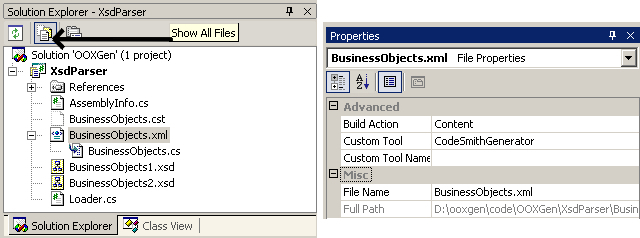
\includegraphics[width=11cm]{./files/inc/figures/codesmithVsdotnet}
				\caption{\label{fig:vsdotnetCustomTool}Visual Studio .NET integration}
			\end{center}
		\end{figure}
		
		If the option \emph{Show All Files} (see Figure \ref{fig:vsdotnetCustomTool}) is 
		turned on, the generated file is displayed as a child of the xml file.
	
	\section{Working with the Application}
		Now, everything is created and ready to use. To actually use the code we need a
		client application which uses the generated classes. This can be of any
		complexity and size. For this example, we use a very basic console
		application. Listing \ref{lst:sampleApplication} shows the code of the test method.
		First, and important, the program class the registry's \verb~init()~ method.
		Parameters are the running program (this) and the host and name of the
		database to be used (line 3).
		After initialisation, the application searches all persons in the database.
		Next, a specific person is searched. That is, the person with the Id 2. All
		orders for this person are wrote to the console. To finish the sample
		program, a new order for this person is created. This order is added to 
		the person and changed afterwards.
		
		After everything has been done, a commit on the unit of work is called.
		This executes all operations on the database.
		
		\begin{lstlisting}[language={[Sharp]C},caption=Sample console application,
		label=lst:sampleApplication]
public void test()
{
	Registry.Instance.init(this, "localhost", "OrderApplication");

	IList persons = (Person.PersonFinder)Registry.Instance.
		getFinder(typeof(Person)).findAll();

	Person person = (Person)Registry.Instance.
		getFinder(typeof(Person)).findById(new Key(new object[] {2}));
	
	foreach(Order order in person.Orders)
	{
		Console.WriteLine(order);
	}

	Order order = ((Order.OrderFactory)Registry.Instance.
		getFactory(typeof(Order))).
		createOrder(person, new DateTime(2003, 12, 1), null, "");
		
	person.addOrder(order);

	order.ShippedDate = DateTime.Today;
	
	UnitOfWork.Instance.commit();
}
		\end{lstlisting}
		
		Although this is a very simple application, it should give an impression how
		fast an application can be build using \textit{STORM}. A great advantage
		of using a generative programming technique is, that even if an application
		becomes larger, there is not much extra work to do. The only thing which 
		needs to be done is to implement another abstract class.
		
%\chapter{Conclusion}
	\section{Specific}
	A generative programming technique can be very powerful if used in the right context.
	Even though, it has its limitations, at least where productivity
	is concerned. One important thing is to precisely
	define the scope and the target when developing a tool such as \textit{STORM}.
	That is, it is important to know what the application which should be generated at the
	end needs to do. For example, to write templates for \textit{STORM} that can be used in 
	\emph{any} project which uses a database is nearly impossible. At least it would lack the
	whole benefit of code generation. Namely these benefits are that an application
	can be build in a much shorter time and the resulting application is error-free.
	But if every possible requirement had to be covered by the template, it would
	likely take a longer time to develop it than it ever can save.
	
	\section{In General}
	In general, a generative programming technique is useful whenever the 
	requirements for a project can be accurately specified from the beginning
	and do not change very much. Furhtermore, the project needs to be of
	a certain extend because it is doubtful if its worth the effort to create
	a framework for code generation just for a small application.
	
	The conclusion therefore is that code generation can help very much to shorten
	development time and to improve code quality. This, of course, is not limited
	to an object/relational mapper.
	
	\section{Outlook}
	\textit{STORM} could be extended in many ways. One important thing would be
	to implement different locking mechanism, another to support all database
	mapping types. Another extend would be to generate code for web service facade
	to domain object mappings.
	Although \textit{STORM} does not support this, it should give a reasonable start 
	for further development. 

\selectlanguage{ngerman}

\part{Manuals}
\label{par:manuals}
\vspace{2cm}
Der folgende Teil enth�lt Kapitel in Deutsch und Englisch. Wir haben entschieden, nur den technischen Bericht in Englisch zu verfassen, hatten zu diesem Zeitpunkt jedoch schon einzelne Kapitel geschrieben.

\selectlanguage{english}
\chapter{CodeSmith}
\label{cha:codeSmith}


%----------
\section{Template Syntax}
CodeSmith \cite{CodeSmith} is a freeware template-based code generator which is able to 
generate code for any ASCII-based language. The syntax for creating 
CodeSmith templates is close to the ASP.NET syntax.

A template source file consists of template code and the static part of the 
desired source code output. In Listing \ref{lst:simpleExample} you can see 
an example. Everything encapsulated in \verb~<% %>~ tags will be 
replaced by CodeSmith, the rest be printed as is.

There are varieties of this tags. \verb~<%@~ is the beginning of a 
compiler directive. On the line 1 of Listing \ref{lst:simpleExample} you 
can see the \verb~CodeTemplate~ directive. This is the first and only 
mandatory code block in a template. It needs a \verb~Language~ attribute 
specifying the template language and a \verb~TargetLanguage~ attribute 
defining the language of generated code output. A \verb~Description~ 
attribute can be given optionally.

The \verb~Property~ directive you see at line 3 declares a property 
with a \verb~Name~ and a \verb~Type~ as mandatory attributes. This is exactly 
the same as a .NET property. The attribute \verb~Category~ defines
the Section where the property is shown in the GUI. The given category on 
line 3 of Listing \ref{lst:simpleExample} can be found in the section title 
of the \verb~ClassName~ property in Figure \ref{fig:codesmithGUI}. If no 
category is specified the property will be shown in the misc section.

\begin{lstlisting}[float,caption=Simple Example,label=lst:simpleExample]
<%@ CodeTemplate Language="C#" TargetLanguage="C#"
                 Description="This is a sample template." %>
<%@ Property Name="ClassName" Type="System.String" Category="Design"
             Default="MyClass1" Description="Name of class to create" %>

public class <%= ClassName %>() {

   <%= ClassName %>() {
   }
}
\end{lstlisting}

A code block beginning with \verb~<%=~ contains only one property like at 
lines 6 and 8 in Listing \ref{lst:simpleExample}. It is a short form to 
print that property. You can see the result of the template code in Listing 
\ref{lst:simpleExample} in Figure \ref{fig:codesmithGUI}.

\begin{figure}[H]
	\begin{center}
		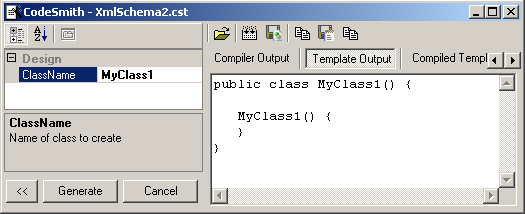
\includegraphics[width=9cm]{./files/inc/figures/codesmithGUI}
		\caption{\label{fig:codesmithGUI}CodeSmith GUI}
	\end{center}
\end{figure}


%-----
\subsection{Functions}
Template code can contain any logic like a loop for iterating, an 
\verb~if~ clause or anything else. If code is too complex to manage 
in a template there is the possibility to write functions. Usually 
they are placed at the end of a template in a \verb~<script>~ section 
as shown in Listing \ref{lst:script}.

\begin{lstlisting}[float,caption=$<$script$>$ section,label=lst:script]
<script runat="template">
public string getEmail(string forename, string name)
{
	string email = forename + "." + name + "@hsr.ch";
	return email;
}
</script>\end{lstlisting}


%-----
\subsection{Derive from ``code behind''}
For more complex templates it could be useful to split the code into two 
files. The template file will only consists of static text and as few logic 
as possible. Only some simple loops or decisions. The main logic can be 
packed into a class placed in an external file. Such code is called ``code 
behind'' because you don't see it while working on the template.

This class has to be derived from the \verb~CodeTemplate~ class in the namespace 
\verb~CodeSmith.Engine~ as shown in Listing \ref{lst:codebehind} at line 1 and 5. The 
code template has to inherit from this class. How to reference the external 
file in the template and inherit from the class in it is shown in Listing 
\ref{lst:derive}.

\begin{lstlisting}[caption=Code behind (sample1.cst.cs),label=lst:codebehind]
using CodeSmith.Engine;

namespace SampleNamespace
{
	public class Sample1 : CodeTemplate
	{
		private string className;
		
		public Sample1() { }
		
		public string ClassName {
			get{ return value; }
			set{ className = value; }
		}
	}
}
\end{lstlisting}

\begin{lstlisting}[caption=Include a base class (sample1.cst),label=lst:derive]
<%@ CodeTemplate Src="sample1.cst.cs" Inherits="SampleNamespace.Sample1"
                 Language="C#" TargetLanguage="C#" %>
                 
public class <%= ClassName %>() {

   <%= ClassName %>() {
   }
}
\end{lstlisting}

Properties in a class you derive from must implement \verb~set~ and \verb~get~ 
methods because CodeSmith treats such a property like those declared with 
directives. CodeSmith has to read them to show the values in the GUI. And it 
has to manipulate them if you change a value over the GUI or generate code 
with an external configuration as described later.

All the properties and methods in such a class can be accessed directly from 
inline code as you see in Listing \ref{lst:derive} at line 4 and 6.


%-----
\subsection{Logic in an assembly}
Another possibility to separating the logic from template code is to use an 
assembly. Listing \ref{lst:assemblyTpl} shows the usage of an assembly. 
There are two directives needed. The directive at line 3 specifies an assembly 
without the .dll extension. It needs to be in either the same directory as the 
template or in the same directory as the CodeSmith executable.

Now you can make instances of each class in that assembly. The line 2 in Listing 
\ref{lst:assemblyTpl} shows how to make an instance of the class \verb~Sample2~ 
in the namespace \verb~SampleNamespace~. The property \verb~FileObject~ represents 
the instance. You can access all properties and methods of this object like shown 
in line 7 of Listing \ref{lst:assemblyTpl}

\begin{lstlisting}[float,caption=Use an Assembly,label=lst:assemblyTpl]
<%@ CodeTemplate Language="C#" TargetLanguage="C#" %>
<%@ Property Name="FileObject" Type="SampleNamespace.Sample2" %>
<%@ Assembly Name="ASample" %>

public SampleClass {
  public static void main() {
    Console.WriteLine("Selected file: {0}", <%= FileObject.File %>);
  }
}
\end{lstlisting}

The property defined in the template in that case is an object. This object can have 
several properties. That is why it is needed to implement an \verb~Editor~, which enables 
you to set the properties of that object with the CodeSmith GUI. Such an \verb~Editor~ is a 
.NET technologie to edit the properties of an object which is bound to a input field 
in a GUI. If you bind your own object to an input field you have to write your own 
\verb~Editor~.

For this the assembly must provide a form for a modal dialog or a drop-down box 
which is designed to set all the properties. To show the settings in the GUI, 
CodeSmith calls the \verb~ToString()~ method. To have any effect on the text showed 
in the GUI you can overwrite the \verb~ToString()~ method.

Listings \ref{lst:assemblyClass} and \ref{lst:assemblyClassEditor} use a 
default \verb~OpenFileDialog~ to demonstrate this functionality. Line 6 and 7 
of Listing \ref{lst:assemblyClass} is defined which \verb~Editor~ to use. Listing 
\ref{lst:assemblyClassEditor} shows the implementation of such an \verb~Editor~.

\begin{lstlisting}[caption=Assembly source,label=lst:assemblyClass]
using System;
using System.ComponentModel;

namespace SampleNamespace
{
	[Editor(typeof(SampleNamespace.Sample2Editor),
	        typeof(System.Drawing.Design.UITypeEditor))]
	public class Sample2 
	{
		private string m_file = "";

		public Sample2()
		{
		}

		public string File 
		{ 
			get { return m_file; } 
			set { m_file = value; } 
		}
	
		public override string ToString() {	return m_file; }
	}
}
\end{lstlisting}

\begin{lstlisting}[caption=Editor,label=lst:assemblyClassEditor]
using System;
using System.ComponentModel;
using System.Windows.Forms;
using System.Drawing.Design;

namespace SampleNamespace
{
	public class Sample2Editor : UITypeEditor
	{
		public Sample2Editor() : base() {}

		public override object EditValue(ITypeDescriptorContext context,
		                                 IServiceProvider provider,
		                                 object obj) 
		{
			if (provider != null)
			{
				OpenFileDialog fileDialog = new OpenFileDialog();

				if(fileDialog.ShowDialog() == DialogResult.OK)
				{
					obj = new Sample2();
					((Sample2)obj).File = fileDialog.FileName;
				}
			}
			return obj;
		}

		public override
		UITypeEditorEditStyle GetEditStyle(ITypeDescriptorContext context) 
		{
			return UITypeEditorEditStyle.Modal;
		}
	}
}
\end{lstlisting}

If you click into the input field in the CodeSmith GUI the method 
\verb~EditValue()~ will be called. This opens the \verb~FileOpenDialog~ 
and sets the property \verb~File~ after closing the dialog.

The method \verb~GetEditStyle()~ tells the CodeSmith GUI what kind of input 
box to provide. Either a drop-down box or a modal dialog are possible. For 
the \verb~FileOpenDialog~ you have to set \verb~Modal~ (see Listing 
\ref{lst:assemblyClassEditor},line 32). This results in a button with three 
dots like you can see next to the input box of \verb~FileObject~ in Figure 
\ref{fig:codesmithGUI2}.

\begin{figure}[thb]
	\begin{center}
		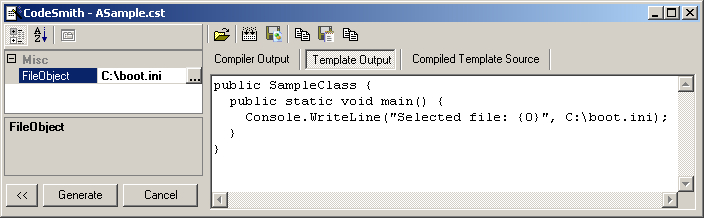
\includegraphics[width=12cm]{./files/inc/figures/codesmithGUI2}
		\caption{\label{fig:codesmithGUI2}Input box for an assembly}
	\end{center}
\end{figure}


%----------
\section{Code generation}
\label{sec:codeSmithGeneration}

If you want to generate code for several values it is a drawback that you have 
to set all the properties by hand. That's why you can can use an external file 
as input for the generation process. This procedure is described in the 
following section.


%-----
\subsection{XML configuration file}
There are two ways to generate code without the CodeSmith GUI. You can choose between 
a command line tool and the possibility to 
integrate the generation into Microsoft Visual Studio .NET. Both take 
the settings from an xml file like in Listing \ref{lst:xmlConfig}. 

The specified \verb~namespace~ at line 3 is optional and encloses the whole 
generated code from all defined \verb~propertySet~s.
The \verb~imports~ given at lines 5 and 6 are included at the top of the generated 
code with the \verb~using~ keyword.
For each \verb~propertySet~ defined in the \verb~propertySets~ element CodeSmith 
generates code with the properties specified in it.

\begin{lstlisting}[float,language=XML,caption=xml configuration,label=lst:xmlConfig]
<?xml version="1.0" encoding="utf-8" ?>
<codeSmith>
	<namespace>MyNamespace</namespace>
	<imports>
		<import namespace="System" />
		<import namespace="System.Collections" />
	</imports>
	<propertySets>
		<propertySet>
			<property name="FileName">BusinessObj1.dll</property>
		</propertySet>
		<propertySet>
			<property name="FileName">BusinessObj2.dll</property>
		</propertySet>
	</propertySets>
	<template path="BusinessObjects.cst" />
</codeSmith>
\end{lstlisting}

\noindent The command line to generate code is:\\
\indent \verb~CodeSmithConsole.exe sample1.xml output.cs~

\noindent The first filename specifies the xml configuration file. The second filename 
is optional. If specified, the generated code is written to that file, otherwise 
the output is shown on stdout. 

%-----
\subsection{Visual Studio .NET integration}
To run the generation of code from within the Visual Studio you have to add the xml 
configuration file to the Visual Studio project. Then you have to set the 
property \verb~Custom Tool~ to \verb~CodeSmithGenerator~ as shown in Figure 
\ref{fig:codesmithVsdotnet} on the right.

The \verb~Build Action~ field has to be set to \verb~Content~. This causes Visual Studio 
to execute the generation every time the content of the xml file has changed. The generation 
of the code can also be initiated by right clicking the xml file and select 
\verb~Run Custom Tool~.

\begin{figure}[thb]
	\begin{center}
		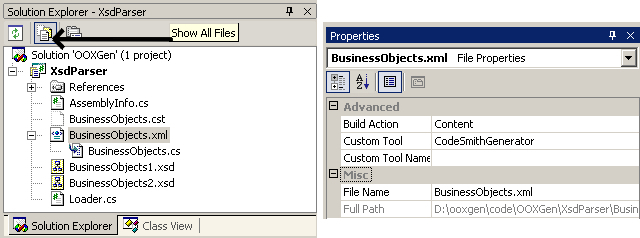
\includegraphics[width=11cm]{./files/inc/figures/codesmithVsdotnet}
		\caption{\label{fig:codesmithVsdotnet}Visual Studio .NET integration}
	\end{center}
\end{figure}

If the option \emph{Show All Files} (see Figure \ref{fig:codesmithVsdotnet}) is 
turned on, the generated file is displayed as a child of the xml file.
\selectlanguage{ngerman}
\chapter{STORM}
	
	\section{Einleitung}
		Dieses Kapitel gibt eine Anleitung dazu, wie eine Applikation mit \textit{STORM}
		erstellt werden kann. Der Grund daf�r ist, dass die Verwendung der Attribute
		nicht ganz selbsterkl�rend ist. Die Attribute selbst wurden im technischen
		Bericht bereits beschrieben. Das wird hier nicht wiederholt.
		
	\section{Vorbereitung}
		\subsection{CodeSmith}
			Zuerst muss CodeSmith auf dem Rechner installiert werden. Das Tool kann
			von \url{http://www.ericjsmith.net/codesmith/download.aspx} bezogen werden.
			Die Installation selbst sollte kein Problem darstellen.
		
		\subsection{Projekt erstellen}
			Als n�chster Schritt wird ein neues Projekt oder eine neue Solution vom
			gew�nschten Typ im Visual Studio .NET erstellt. Vorteilhaft ist es, wenn
			im neuen Projekt ein Ordner f�r die Domain Objekte angelegt wird. Dies ist 
			zwar nicht n�tig, aber dient der besseren �bersicht. Ebenso ist es n�tzlich,
			gleich einen Ordner f�r die Domain Objekt Implementationen und f�r die 
			Mapper Implementation zu machen.
			
		\subsection{Library und Templates}
			\textit{STORM} beinhaltet zwei Templates, die f�r die Code Generierung ben�tigt
			werden. Dies sind \verb~ImplGen.cst~ und \verb~MapperGen.cst~. Diese k�nnen 
			grund\-s�tzlich	�berall auf der lokalen Festplatte liegen. Es ist aber wiederum 
			ratsam, einen	eigenen Ordner im aktuellen Projekt zu erstellen und die beiden 
			Dateien in diesen Ordner zu kopieren.
			
			Des weiteren muss die STORM-Library (\verb~Storm.dll~) in das von CodeSmith erstellte
			Verzeichnis kopiert werden. Dies ist leider n�tig, da CodeSmith bei der Code Generierung
			auch dann die Dll nicht findet, wenn sie im GAC registriert wurde. Aktuell ist dieses
			CodeSmith Verzeichnis:
			\begin{Verbatim}
C:\Program Files\CodeSmith\v2.2\
			\end{Verbatim}
			Dies kann aber je nach lokalen Einstellungen und CodeSmith Version variieren.
			
			Um eine Applikation mit \textit{STORM} entwickeln zu k�nnen, muss die Library zus�tzlich vom aktuellen
			Projekt referenziert werden. Dazu wird die Datei (\verb~Storm.dll~) im Visual Studio .NET
			unter dem Punkt \verb~References~ $\rightarrow$ \verb~Add References...~ $\rightarrow$
			\verb~Browse~ angegeben.
			
			Figur	\ref{fig:vsdotnetSolutionExplorer} ist ein Beispiel wie eine Solution nach 
			diesen Schritten aussehen sollte.
		
			\begin{figure}[htb]
				\begin{center}
					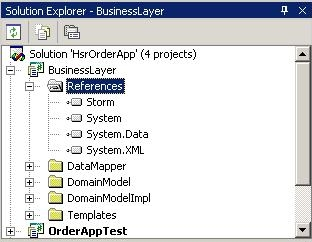
\includegraphics[width=4.5cm]{./files/inc/figures/vsdotnetSolutionExplorer}
					\caption{\label{fig:vsdotnetSolutionExplorer} Solution Explorer nach der Vorbereitung}
				\end{center}
			\end{figure}		
		
		\section{Abstrakte Klassen}
		
			Wenn alle Vorbereitungen abgeschlossen sind, kann man beginnen, die abstrakten Klassen 
			zu schreiben. Nat�rlich muss vorher das Design der Applikation feststehen.
			F�r jede Tabelle in der Datenbank muss eine Abstrakte Klasse geschrieben werden.
			Diese Klasse wird nachher mit den von \textit{STORM} definierten Attributen versehen.
			
			\subsection{�bersicht}
				Hier eine �bersicht der behandelten Themen in diesem Kapitel:
				\LTXtable{\linewidth}{./files/inc/tables/manualThemen}
				
			
			\subsection{Namespaces}
			\label{subsec:manualNamespaces}
				Um mit den von \textit{STORM} angebotenen Klassen arbeiten zu k�nnen, m�ssen als Erstes zwei
				Namespaces in der abstrakten Klasse eingebunden werden:
				\begin{lstlisting}[language={[Sharp]C},caption=Namespaces einbinden,
					label=lst:namespaces]
using Storm.Attributes;
using Storm.Lib;
				\end{lstlisting}
			
			\subsection{Klassen-Attribute}
			\label{subsec:manualKlassen}
				Es gibt verschiedene Typen von Attributen. Einige sind f�r die Attributierung
				der Klassen vorgesehen, andere f�r Methoden, etc.
				Hier beginnen wir sinnvollerweise mit der Attributierung einer abstrakten Hauptklasse.
				Die Bezeichnung Hauptklasse verwenden wir deshalb, weil es Klassen innerhalb dieser
				Klasse geben kann. Die folgende Liste beschreibt alle Attribute die f�r eine Hauptklasse
				verwendet werden. Es m�ssen alle Attribute angegeben werden.
				
				\begin{itemize}
					\item Table(string tableName, bool keyIsSurrogate)\\
					Wird ben�tigt um das Mapping zwischen einer Klasse und einer Tabelle zu machen. Zu jeder Klasse
					geh�rt eine Tabelle in der Datenbank.
					\begin{description}
						\item[tableName] Der Name der Tabelle in der Datenbank, auf die diese Klasse gemappt werden soll.
						\item[keyIsSurrogate] Definiert ob ein Key surrogate, also k�nstlich ist oder nicht. Falls \verb~true~
																	angegeben wird, darf in der Klasse nur ein Primary Key definiert werden. Ansonsten
																	d�rfen mehrere Primary Keys definiert werden.
					\end{description}
					\item VersionField(string fieldName)\\
					Das Versionen Feld wird ben�tigt um die Aktualit�t der gespeicherten Objekte zu �berpr�fen.
					\begin{description}
						\item[fieldName] Der Name des Feldes in der Datenbank. Erwartet wird hier ein Feld vom Typ 
														 \verb~timestamp~. Dies entspricht einer bin�ren Nummer, die garantiert �ber 
														 die ganze Datenbank eindeutig ist.
					\end{description}
					\item GenerateCode()\\
					Dieses Attribut wurde zur Sicherheit eingef�hrt. Es muss angegeben werden, falls Code
					f�r diese Klasse generiert werden sollte. Falls dieses Attribut fehlt, wird die Klasse
					von \textit{STORM} ignoriert.
				\end{itemize}
				
				Listing \ref{lst:hauptklasse} zeigt ein Beispiel f�r eine Deklaration einer Hauptklasse.
				Zu Beachten ist dabei auch, dass die Hauptklasse von \verb~DomainObject~ abgeleitet
				sein muss.
				
				\begin{lstlisting}[language={[Sharp]C},caption=Definition einer Hauptklasse,
					label=lst:hauptklasse]
[Table("Persons", true),
VersionField("chTimestamp"),
GenerateCode]
public abstract class Person : DomainObject
{
 ...
}	
				\end{lstlisting}
				
			\subsection{interne Klassen}
			\label{subsec:manualInterneKlassen}
				Wie oben angedeutet, ist es m�glich bzw. n�tig, Klassen innerhalb der Hauptklasse
				zu deklarieren. Dies ist m�glich f�r zwei F�lle:
				\begin{itemize}
					\item Eine Factory Klasse kann deklariert werden. Diese wird dazu benutzt, eigene Konstruktoren
								zu erstellen. Falls diese Klasse nicht definiert wurde, kann nur der von \textit{STORM}
								definierte Konstruktor aufgerufen werden.
					\item Eine Finder Klasse kann deklariert werden. Diese Klasse dient dazu, eigene Suchmethoden
								zu definieren. Von \textit{STORM} sind die drei Funktionen \verb~find~, \verb~findAll~ und
								\verb~findById~ vordefiniert. Diese k�nnen auch aufgerufen werden, wenn die Finder Klasse nicht
								deklariert wurde. Der \verb~find~ Methode kann ein QueryObject mitgegeben werden. Damit ist dieser
								Aufruf an sich schon sehr flexibel. Trotzdem ist es aber in manchen F�llen angenehmer, eigene
								Methoden aufrufen zu k�nnen.
				\end{itemize}
				
				Factory Klassen m�ssen das Attribute Factory haben. Innerhalb dieser Klasse werden
				selbst definierte Konstruktoren definiert. Zu Beachten gilt, dass die Klasse
				als abstrakt deklariert werden muss. Ein Beispiel f�r eine Factory Klasse ist das
				folgende Listing:
				
				\begin{lstlisting}[language={[Sharp]C},caption=Definition Factory Klasse]
public abstract class Person : DomainObject
{	
	[Factory]
	public abstract class PersonFactory
	{
		public abstract Person createPerson(
			[ParameterDef("Name")] string name,
			[ParameterDef("Password")] string password);
	}
}
				\end{lstlisting}
				
				Es k�nnen beliebig viele solcher Konstruktoren deklariert werden. Damit klar ist, worauf sich
				ein Parameter einer solchen Methode bezieht, muss pro Parameter ein ParameterDef Attribute
				angegeben werden. Die Bedeutung der benutzten Attribute ist Folgende:
				\begin{itemize}
				\item Factory()\\
				Das Attribute gibt an, dass die folgende Klasse eine interne Klasse der Hauptklasse ist
				und dass eine Factory Klasse folgt. In einer Factory Klasse k�nnen selbst definierte Konstruktoren
				deklariert werden.
				\item ParameterDef(string propertyName)\\
				Beschreibt einen Parameter einer Methode. Jedem Parameter muss ein solches Attribut vorangehen.
					\begin{description}
						\item[propertyName] Gibt an, auf welches Property sich dieser Parameter bezieht. Das Property
																muss in der Hauptklasse existieren. Properties sind in Abschnitt 
																\ref{subsec:manualProps} Beschrieben.
					\end{description}
				\end{itemize}
			
			Finder Klassen k�nnen sehr �hnlich deklariert werden. Sie m�ssen ebenfalls abstrakt sein.
			 Ein Beispiel ist nachstehend angegeben:
			
			\begin{lstlisting}[language={[Sharp]C},caption=Definition Factory Klasse]
public abstract class Person : DomainObject
{	
	[Finder]
	public abstract class PersonFinder
	{
		public abstract IList findByNameAndPassword(
			[ParameterDef("Name")] string name,
			[ParameterDef("Password")] string password);
	}
}
			\end{lstlisting}
			
			Im Gegensatz zu den Factory Methoden, muss bei einer Finder Klasse das Finder Attribut angegeben
			werden. Dieses Attribut gibt an, dass die darauf folgenden Klasse selbst definierte
			Finder Methoden enth�lt. Das ParameterDef Attribute wurde bereits beschrieben und muss auch hier
			pro Parameter angegeben werden.
			
		\subsection{Properties}
		\label{subsec:manualProps}
			F�r jede Kolonne in der Datenbank muss ein Property in der abstrakten Klasse deklariert werden.
			Falls ein Property nicht angegeben wird, ist auch die Kolonne in der Datenbank nicht benutzbar.
			Zus�tzlich kann es zu Schwierigkeiten f�hren, falls das Attribut ben�tigt wird (z.B. f�r Relationen).
			Ein Beispiel einer Deklaration eines Property ist folgendes:
			
			\begin{lstlisting}[language={[Sharp]C},caption=Definition eines Property]
[Column("Name")]
public abstract string Name {get; set;}					
			\end{lstlisting}
			
			Properties m�ssen abstrakt sein. Sie werden im generierten Code implementiert. Es kann mit \verb~get;~
			bzw. \verb~set;~ angegeben werden, was von einem Property implementiert werden soll. Falls von einem
			anderen Attribut (z.B. ParameterDef Attribut) auf ein Property verwiesen wird, muss das Property eine
			\verb~set~ Methode haben. Column ist das einzige Attribut das zwingend ist. Die Bedeutung
			ist folgende:
			\begin{itemize}
				\item Column(string dbColumn)\\
				Dieses Attribut wird verwendet, um ein Property auf eine Kolonne in der Datenbank zu mappen.
				\begin{description}
					\item[dbColumn] Der Name der dazugeh�renden Kolonne in der Datenbank.
				\end{description}
			\end{itemize}
			
		\subsection{Primary Key(s)}
		\label{subsec:manualPrimaryKeys}
			Ein Primary Key wird wie ein Property (\ref{subsec:manualProps}) deklariert. Zus�tzlich zu 
			einem gew�hnlichen Property kommt aber noch ein PrimaryKey Attribut hinzu. Falls im Table
			Attribut \verb~isSurrogateKey~ als \verb~false~ gesetzt wurde, k�nnen mehrere
			Properties das Attribut PrimaryKey haben.	Ansonsten darf dieses Attribut nur einmal verwendet
			werden. Dieses Attribut hat keine Parameter.
			Ein Beispiel einer Deklaration eines Primary Keys ist folgendes:
			
			\begin{lstlisting}[language={[Sharp]C},caption=Definition eines Property]
[Column("PersonID"), PrimaryKey]
public abstract int PersonId {get;}
			\end{lstlisting}
			
		\subsection{ToMany Relation}
		\label{subsec:manualToMany}
			Eine ToMany Relation wird ebenfalls mit einem Property deklariert. Es ist aber
			kein Column Attribute n�tig, da diese Relation auf eine andere Klasse verweist.
			Eine ToMany Relation ist eine one-to-many Relation. F�r jede ToMany Relation
			muss es eine Adder Methode (\ref{subsec:manualAdder}) geben.
			
			\begin{lstlisting}[language={[Sharp]C},caption=Definition eines Property]
[ToMany(typeof(Address), "Person")]
public abstract IList Addresses {get;}
			\end{lstlisting}
			
			Die Bedeutung des Attributes ist folgende:
			\begin{itemize}
				\item ToMany(Type relationTo, string relationName)\\
				Dieses Attribut zeigt an, dass es sich beim diesem Property um eine one-to-many Relation handelt.
				\begin{description}
					\item[relationTo] 	Hier muss der Typ der Klasse angegeben werden, auf die sich die Relation bezieht,
															also der to-many Teil der Relation.
					\item[relationName] Dies gibt den Namen des Property in der Klasse an, auf die sich die Relation
															bezieht. In dieser Klasse muss ein Property mit diesem Name existieren. Zudem
															muss dieses Property ein ToOne Attribut besitzen.
				\end{description}
			\end{itemize}
			
		\subsection{ToOne Relation}
		\label{subsec:manualToOne}
			Eine ToOne Relation wird entweder f�r eine back-Referenz einer ToMany Relation oder f�r
			eine one-to-one Relation benutzt. Es muss f�r \emph{jede} ToMany Relation auch eine
			ToOne Relation geben. Das folgende Beispiel zeigt die Verwendung dieser beiden Attribute
			f�r eine Person mit Adressen:
			
			\begin{lstlisting}[language={[Sharp]C},caption=Zusammenhang zwischen ToMany und ToOne Attribut]
public abstract class Person : DomainObject
{
	[Column("PersonID"), PrimaryKey]
	public abstract int PersonId {get;}

	[ToMany(typeof(Address), "Person")]
	public abstract IList Addresses {get;}
}

public abstract class Address : DomainObject
{
	[Column("PersonID"), ToOne(typeof(Person), "PersonId")]
	public abstract Person Person {get; set;}
}
			\end{lstlisting}
			
			Zu Beachten gilt, dass das mit ToOne attributierte Property ein Column Attribute besitzen muss.
			Zus�tzlich muss das Property eine \verb~set~ Methode haben.
			
			Die Bedeutung des ToOne Attributes ist folgende:
			
			\begin{itemize}
				\item ToOne(Type relationTo, string relationName)\\
				Dieses Attribut zeigt an, dass es sich beim diesem Property entweder um eine one-to-one Relation oder
				um eine back-Referenz einer one-to-many Relation handelt. Es muss ein Column Attribut und eine
				\verb~set~ Methode deklariert werden.
				\begin{description}
					\item[relationTo] 	Hier muss der Typ der Klasse angegeben werden, auf die sich die Relation bezieht,
															also der one-to Teil der Relation.
					\item[relationName] Dies gibt den Namen des Property in der Klasse an, auf die sich die Relation
															bezieht. Diese Relation muss sich auf einen Primary	Key beziehen (siehe Beispiel).
				\end{description}
			\end{itemize}
			
		\subsection{Adder Methoden}
		\label{subsec:manualAdder}
		
			Bei ToMany Relationen darf beim Property keine \verb~set~ Methode deklariert werden, da der
			R�ckgabetyp nicht mit dem zu �bergebenden Typ �berein\-stimmt. Aus diesem Grund wurden
			Adder Methoden eingef�hrt. Das bedeutet, es sollte f�r jede ToMany Relation auch 
			eine Adder Methode definiert werden, um tats�chlich Objekte der Relation hinzuf�gen
			zu k�nnen. Die Methode muss abstrakt sein. Ein Beispiel einer Deklaration 
			einer solchen Adder Methode ist folgende:
		
			\begin{lstlisting}[language={[Sharp]C},caption=Zusammenhang zwischen ToMany und ToOne Attribut]
public abstract class Person : DomainObject
{
	[ToMany(typeof(Address), "Person")]
	public abstract IList Addresses {get;}
	
	[Adder("Addresses", "Person")]
	public abstract void addAddress(Address a);		
}
			\end{lstlisting}
		
			Die Bedeutung des Attributes ist folgende:
			
			\begin{itemize}
				\item Adder(string localProperty, string targetProperty)\\
				Dieses Attribut wird in Erg�nzung zu ToMany Relationen verwendet. Es dient dazu Methoden
				deklarieren zu k�nnen, die es erlauben, einer ToMany Relationen Objekte hinzuzuf�gen.
				\begin{description}
					\item[localProperty] 	Der Name des Property, der die dazugeh�rende ToMany Relation deklariert.
																Diese ist in derselben abstrakten Klasse.
					\item[targetProperty] Dies gibt den Namen des Property in der Klasse an, auf die sich die ToMany Relation
																bezieht. Dieser Name ist derselbe, der im ToMany Attribut angegeben wird.
				\end{description}
			\end{itemize}
			
		\subsection{Ein Beispiel}
		\label{subsec:manualExample}
			Da bis jetzt nur Ausschnitte aus der abstrakten Klasse gezeigt wurden, wird hier ein
			zusammenh�ngendes Beispiel einer abstrakten Klasse gegeben. Es ist das Beispiel
			einer Person:
			
			\begin{lstlisting}[language={[Sharp]C},caption=Zusammenhang zwischen ToMany und ToOne Attribut]
[Table("Persons", true),
	VersionField("chTimestamp"),
	GenerateCode]
public abstract class Person : DomainObject
{	
	[Factory]
	public abstract class PersonFactory
	{
		public abstract Person createPerson(
			[ParameterDef("Name")] string name,
			[ParameterDef("Password")] string password);
	}

	[Finder]
	public abstract class PersonFinder
	{
		public abstract IList findByName([ParameterDef("Name")] string name);
		public abstract IList findByNameAndPassword(
			[ParameterDef("Name")] string name,
			[ParameterDef("Password")] string password);
	}

	[Column("PersonID"), PrimaryKey]
	public abstract int PersonId {get;}

	[Column("Name")]
	public abstract string Name {get; set;}

	[Column("Password")]
	public abstract string Password {get; set;}
	
	[ToMany(typeof(Address), "Person")]
	public abstract IList Addresses {get;}

	[ToMany(typeof(Order), "Person")]
	public abstract IList Orders {get;}

	[Adder("Addresses", "Person")]
	public abstract void addAddress(Address a);

	[Adder("Orders", "Person")]
	public abstract void addOrder(Order o);
}		
			\end{lstlisting}
			
		\subsection{Zus�tzliche Methoden}
		\label{subsec:manualAdditionalMethods}
			In der abstrakten Klasse k�nnen nat�rlich auch Methoden implementiert werden. Diese werden
			nicht attributiert und damit von \textit{STORM} ignoriert. Solche Methoden k�nnen
			aber dennoch wie gewohnt benutzt werden.
			
	\section{Generieren und Kompilieren}
		Nachdem alle abstrakten Klassen geschrieben wurden, kann das Projekt kompiliert werden. Falls
		es ohne Fehler kompiliert, k�nnen die Domain Objekt Implementationen und die Mapper
		Implementationen generiert werden. Da es f�r jede erstellte abstrakte Klasse jeweils
		zwei Implementations-Klassen generiert werden, muss es entsprechend viele
		XML Konfigurations-Dateien geben. Wie das aussehen k�nnte ist in Abbildung \ref{fig:vsdotnetFiles} gezeigt.
		
		\begin{figure}[htb]
			\begin{center}
				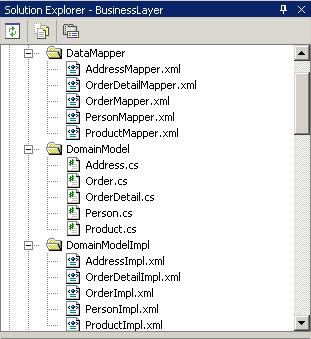
\includegraphics[width=4.5cm]{./files/inc/figures/vsdotnetFiles}
				\caption{\label{fig:vsdotnetFiles} Solution Explorer mit den Konfigurations-Dateien}
			\end{center}
		\end{figure}
		
		Eine Beschreibung um den Code zu generieren ist im CodeSmith Manual ab Abschnitt 
		\ref{sec:codeSmithGeneration} nachzuschlagen.
		
		Nachdem alle Klassen generiert wurden, muss das Visual Studio .NET geschlossen werden. Das
		ist, weil CodeSmith die dll blockiert und deshalb kann nicht mehr darauf zugegriffen werden.
		Nachdem das Projekt wieder ge�ffnet wurde, kann das gesamte Projekt, mit den erstellten Klassen,
		kompiliert werden.
		
	\section{Arbeiten mit dem Projekt}
		Es wurde bereits im technischen Bericht ein Beispiel gegeben, wie die Klassen
		des neu erstellten Projektes benutzt werden k�nnen. Es wird deshalb hier nicht wiederholt, zumal
		die Benutzung auch von den erstellten Abstrakten Klassen abh�ngt. Wichtig ist aber immer,
		dass die generierten Klassen niemals direkt benutzt werden, sonder immer �ber die Factory
		bezogen werden.


\part{Projektplanung}
\label{par:projectManagement}
\vspace{2cm}
	
\chapter{Risiken}
	Neben den �blichen Risiken, die in jedem Projekt bestehen 
	(Krankheit, pers�nliche Probleme, etc.) bestehen folgende
	Risiken:
	\LTXtable{\linewidth}{./files/inc/tables/projektMgmtRisks}
	
\chapter{Projektplan}
	\section{Versionen}
		Die Projektpl�ne sind auf den n�chsten Seiten der Dokumentation beigelegt. Folgende Versionen
		sind verf�gbar:
		\LTXtable{\linewidth}{./files/inc/tables/projektMgmtProjectPlan}
		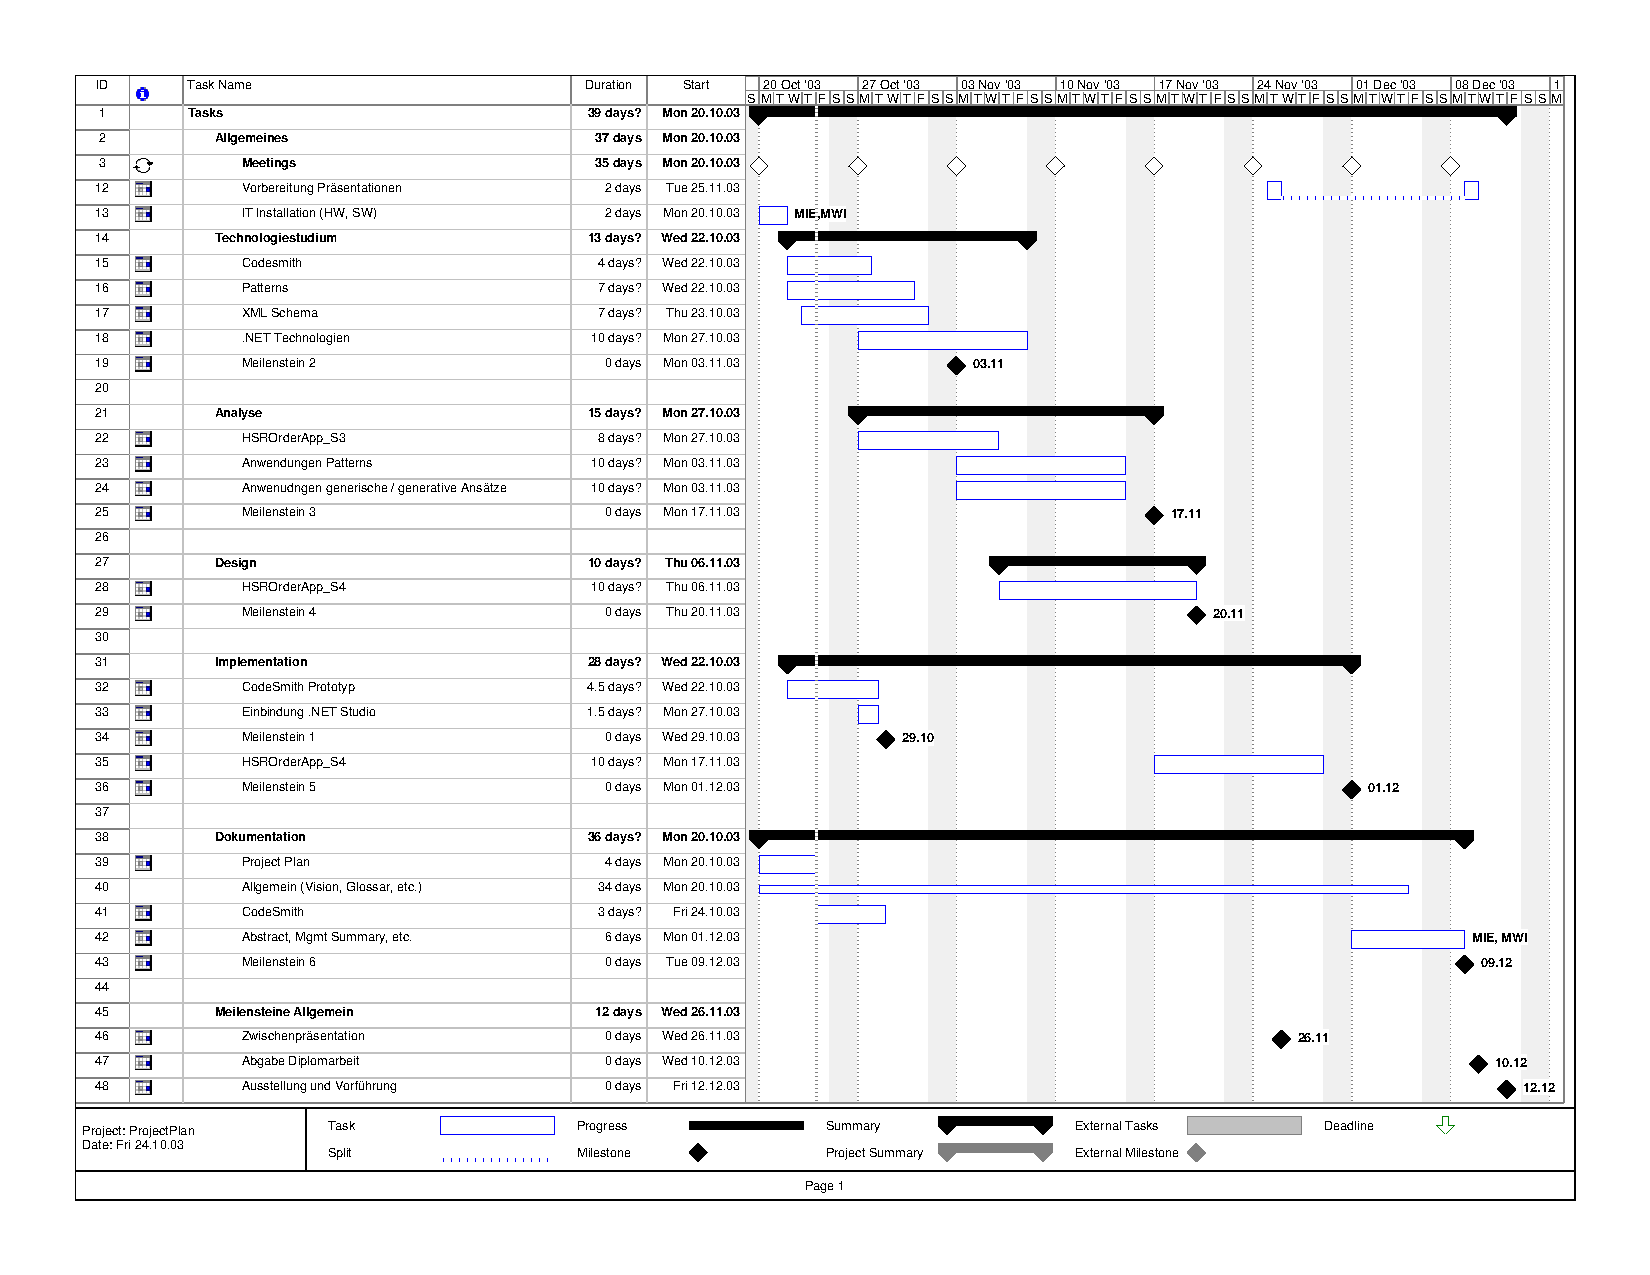
\includepdf[pages={1},landscape]{./files/inc/sources/ProjectPlan_v0-1}
		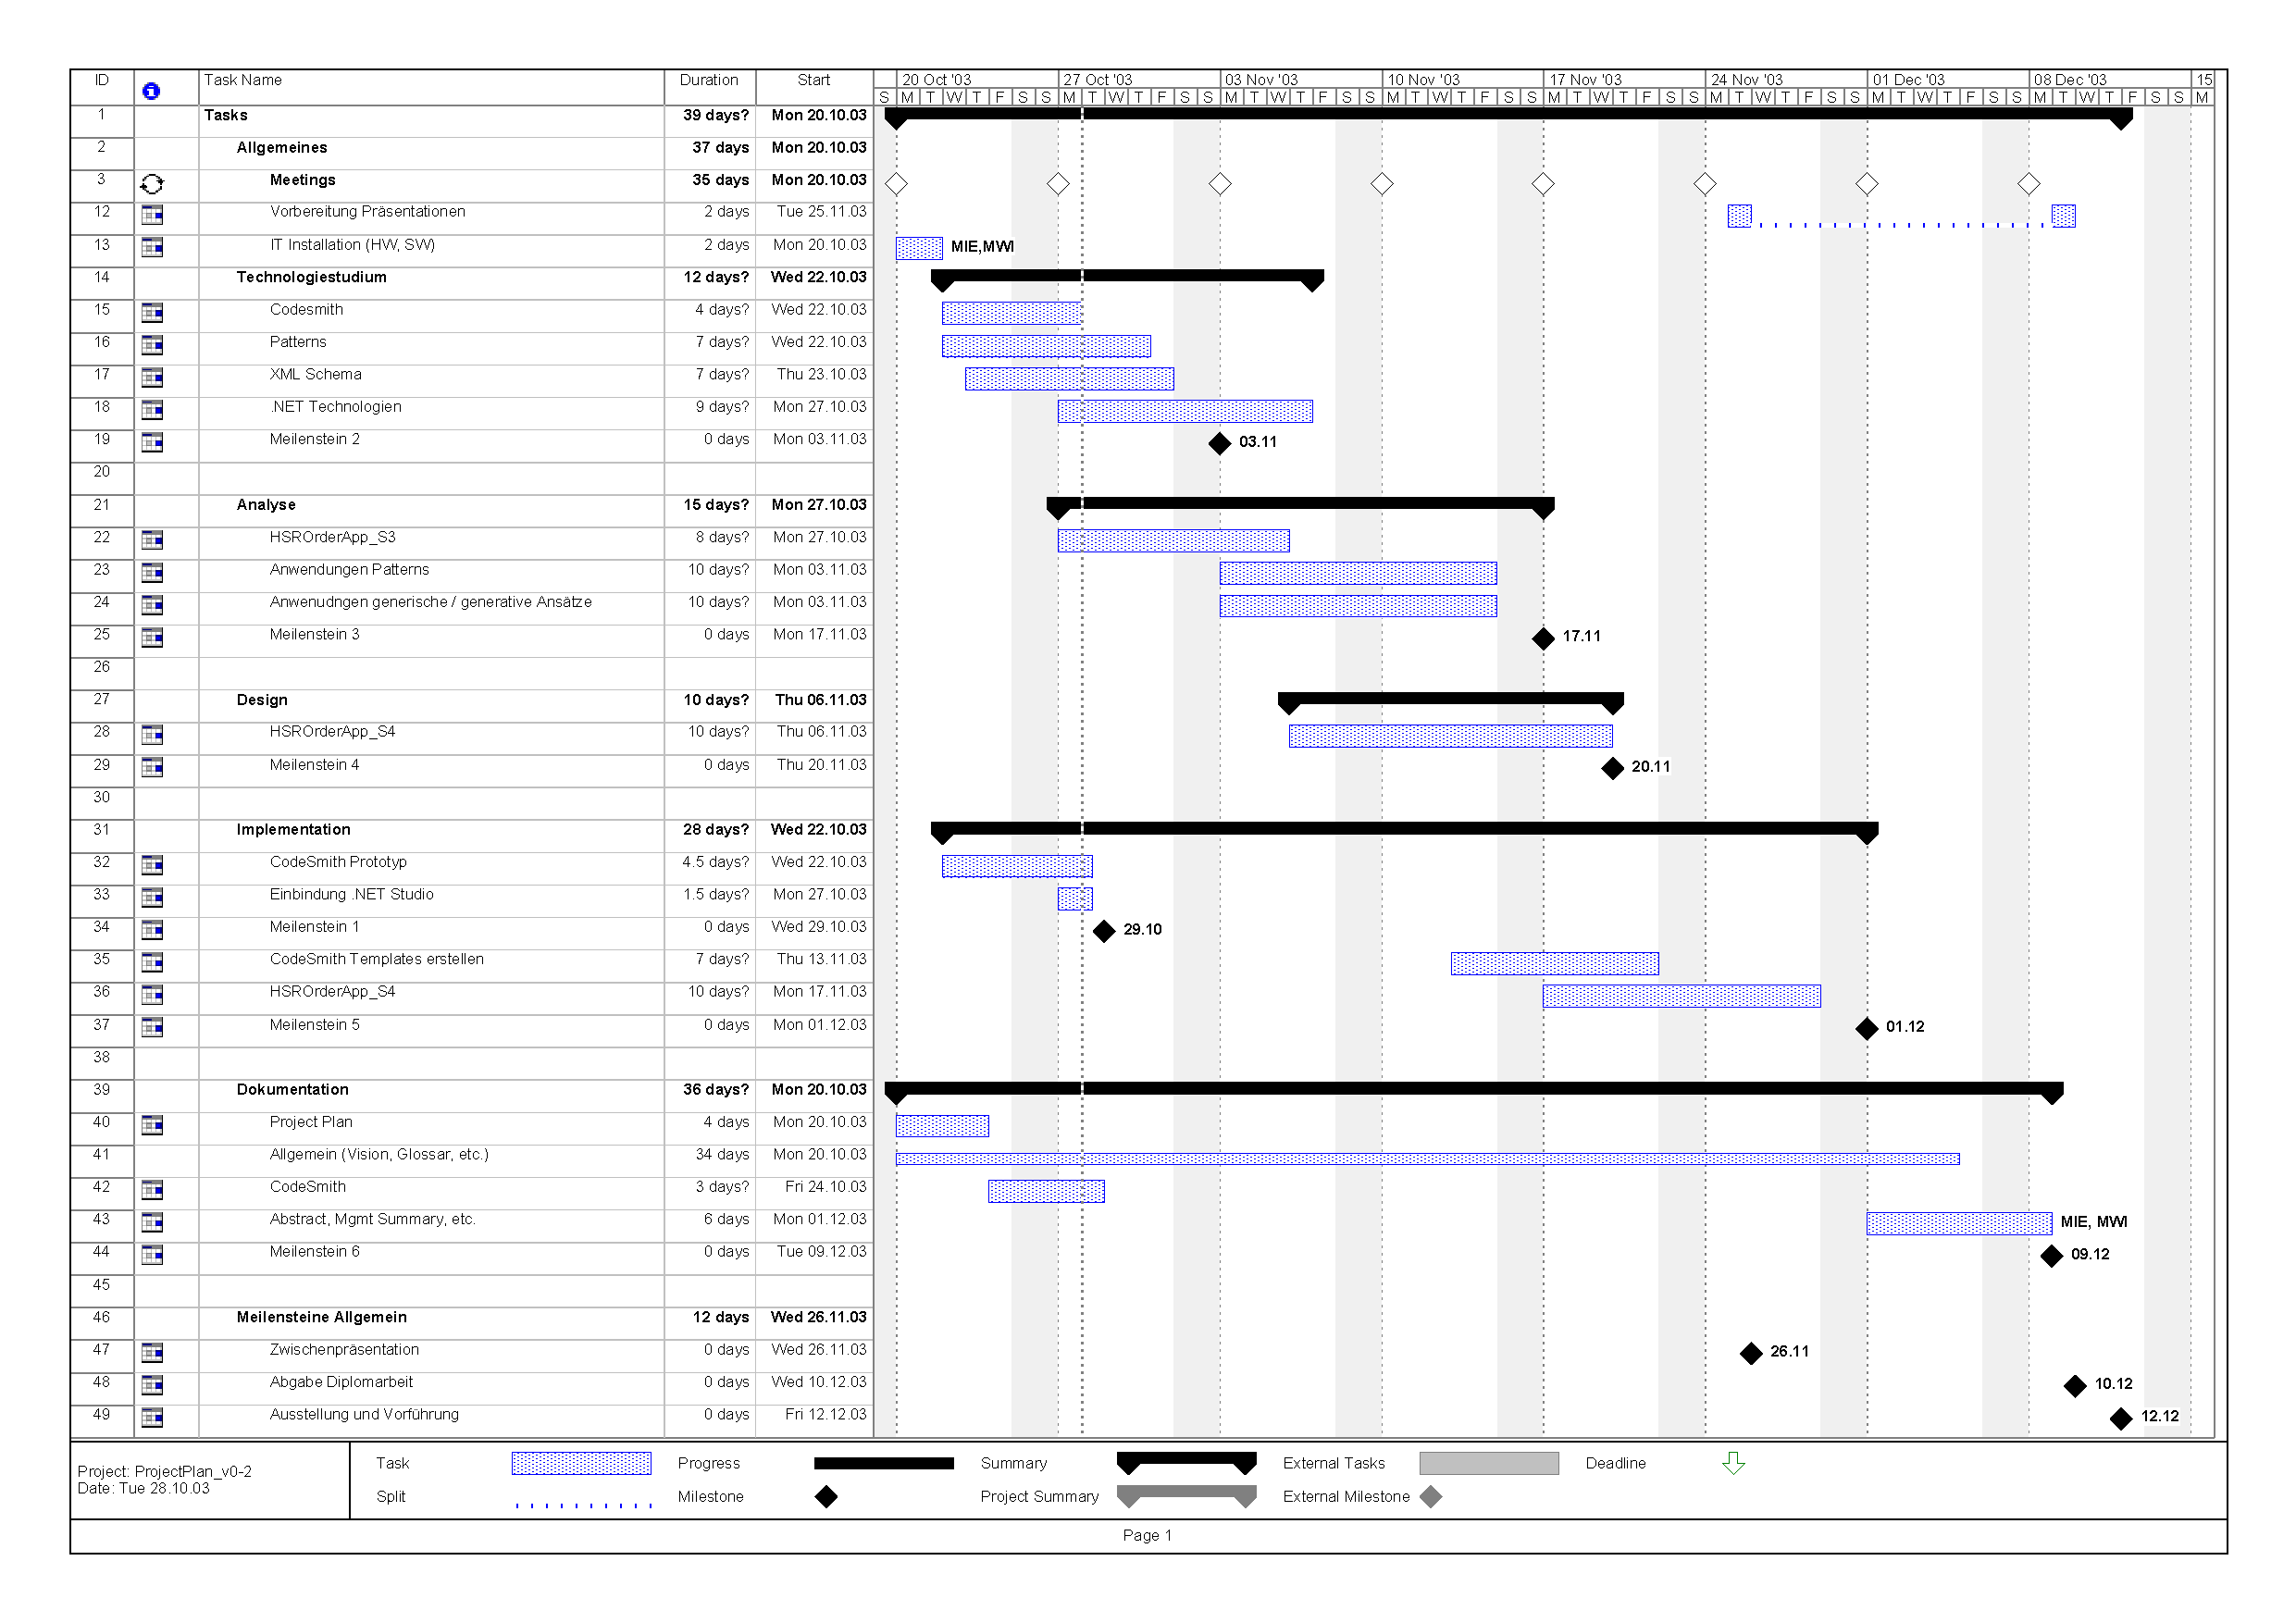
\includepdf[pages={1},landscape]{./files/inc/sources/ProjectPlan_v0-2}
		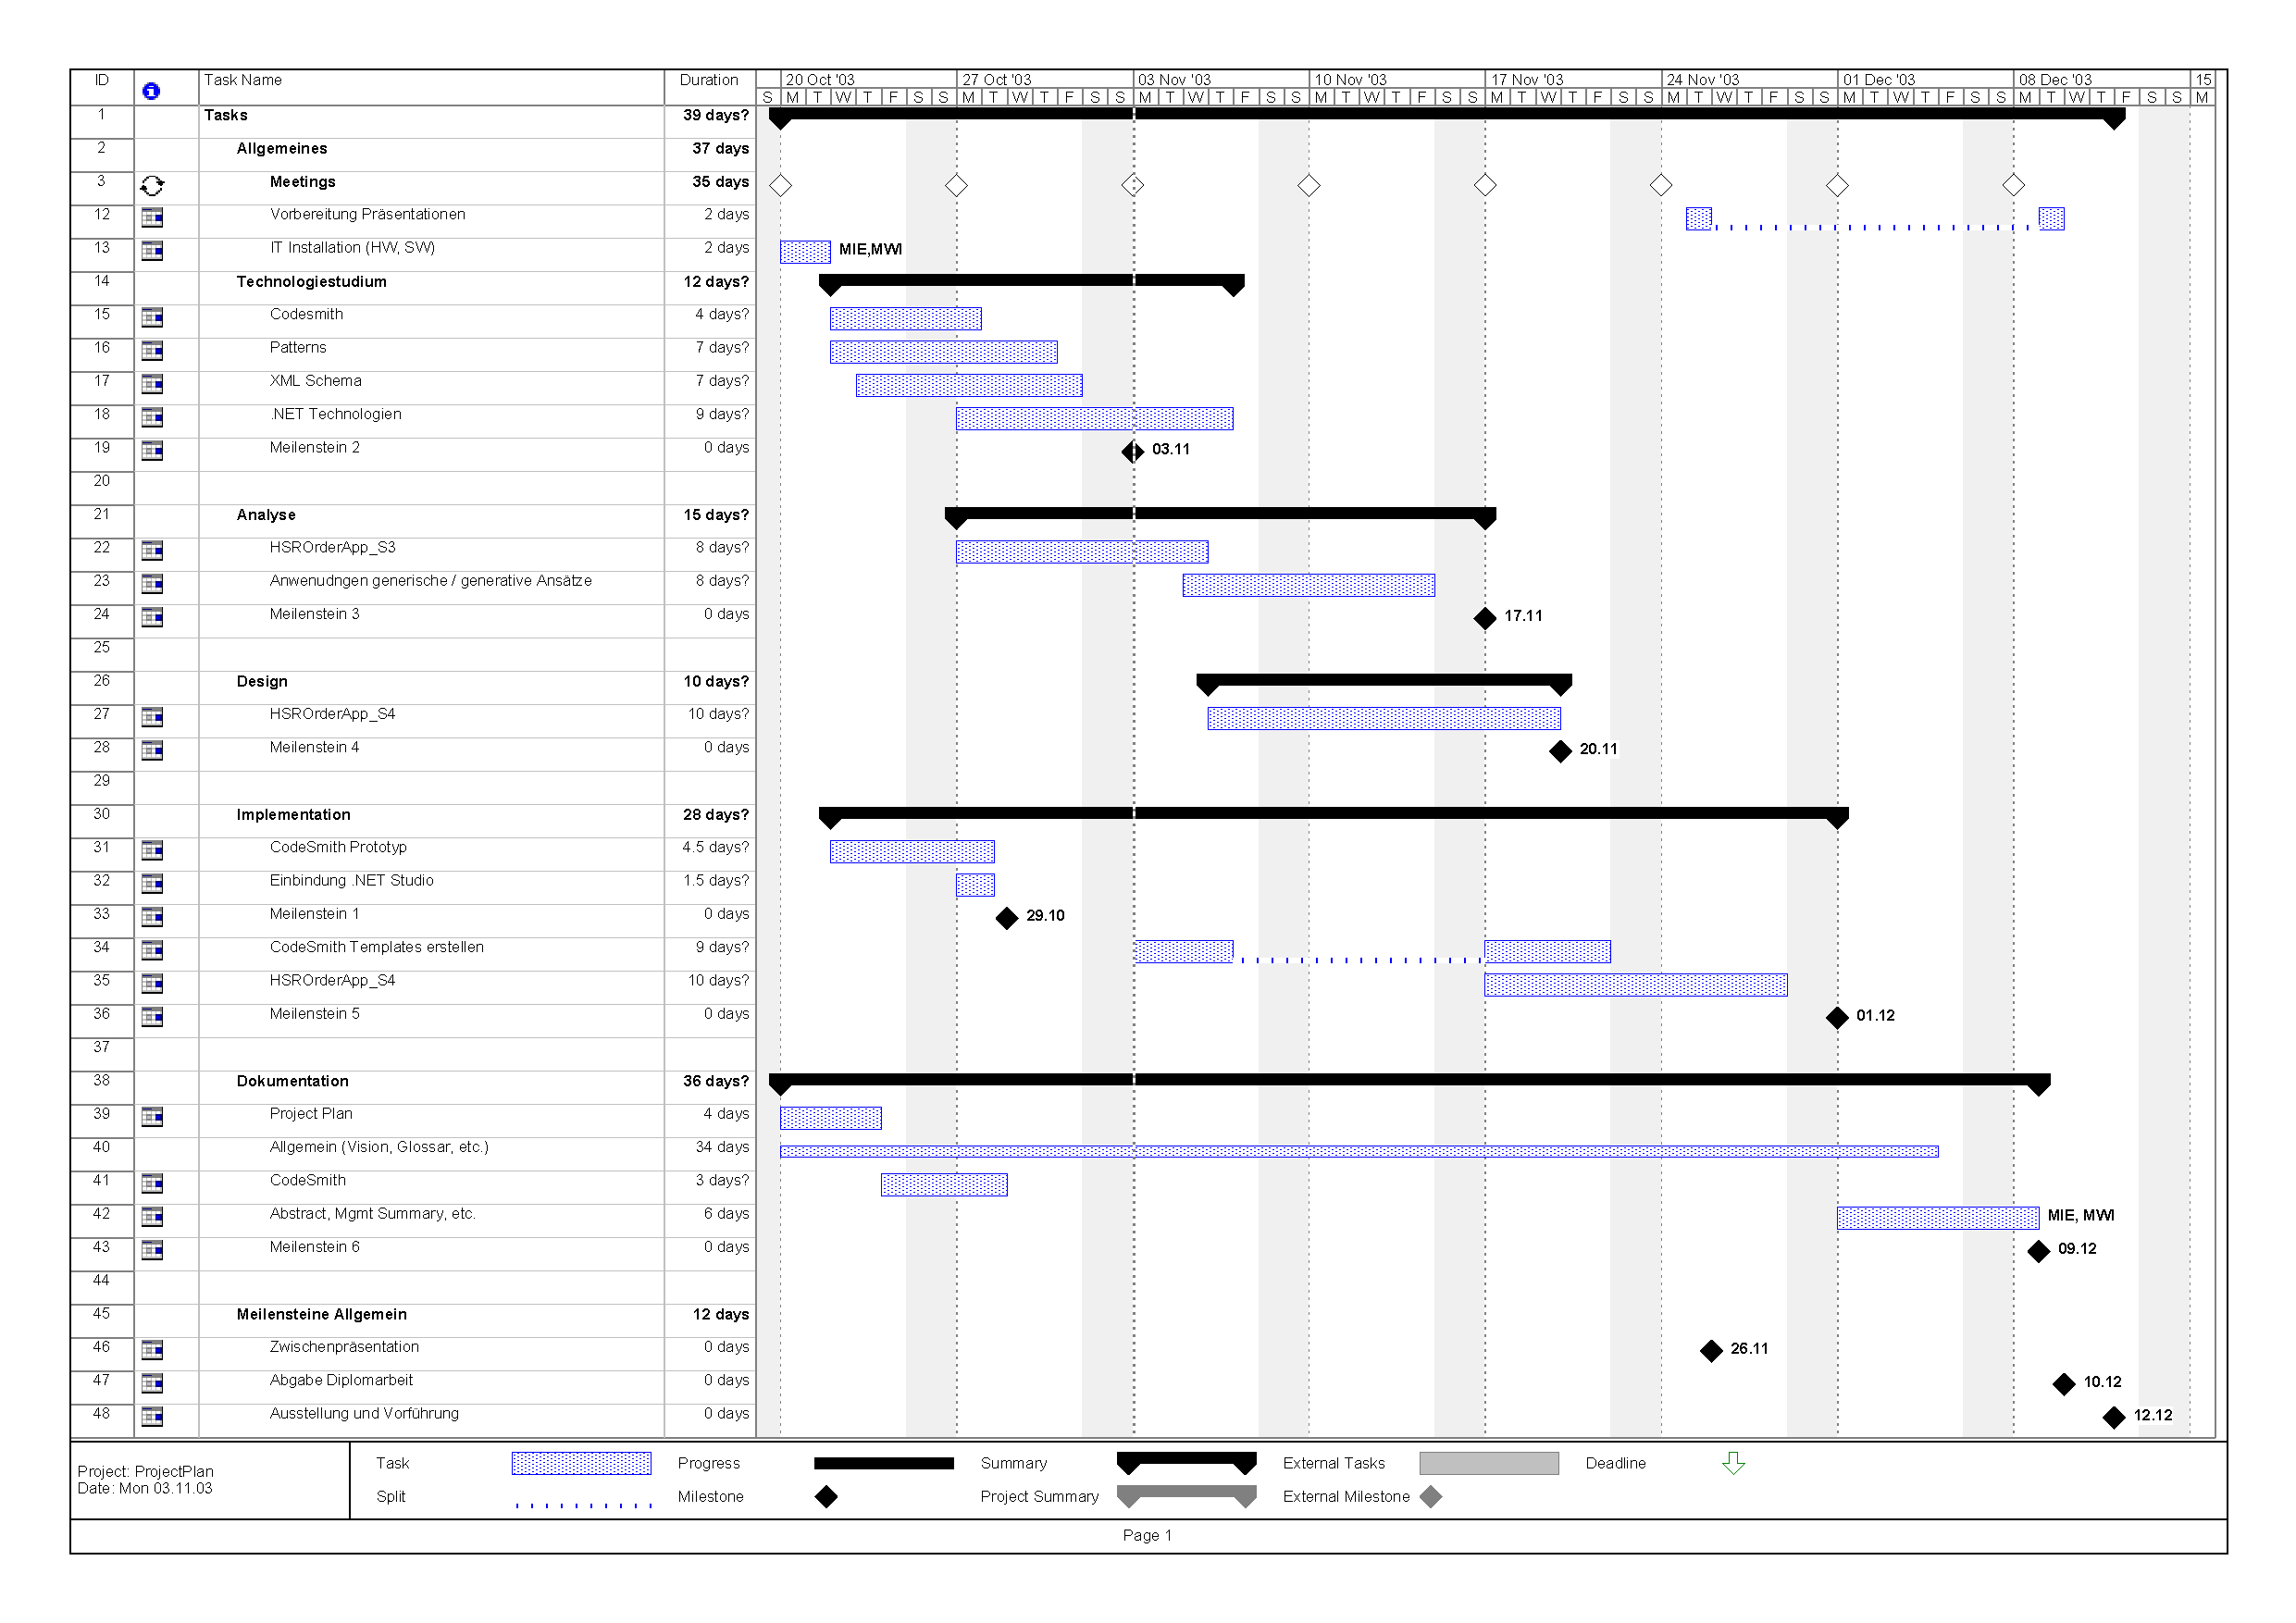
\includepdf[pages={1},landscape]{./files/inc/sources/ProjectPlan_v0-3}
		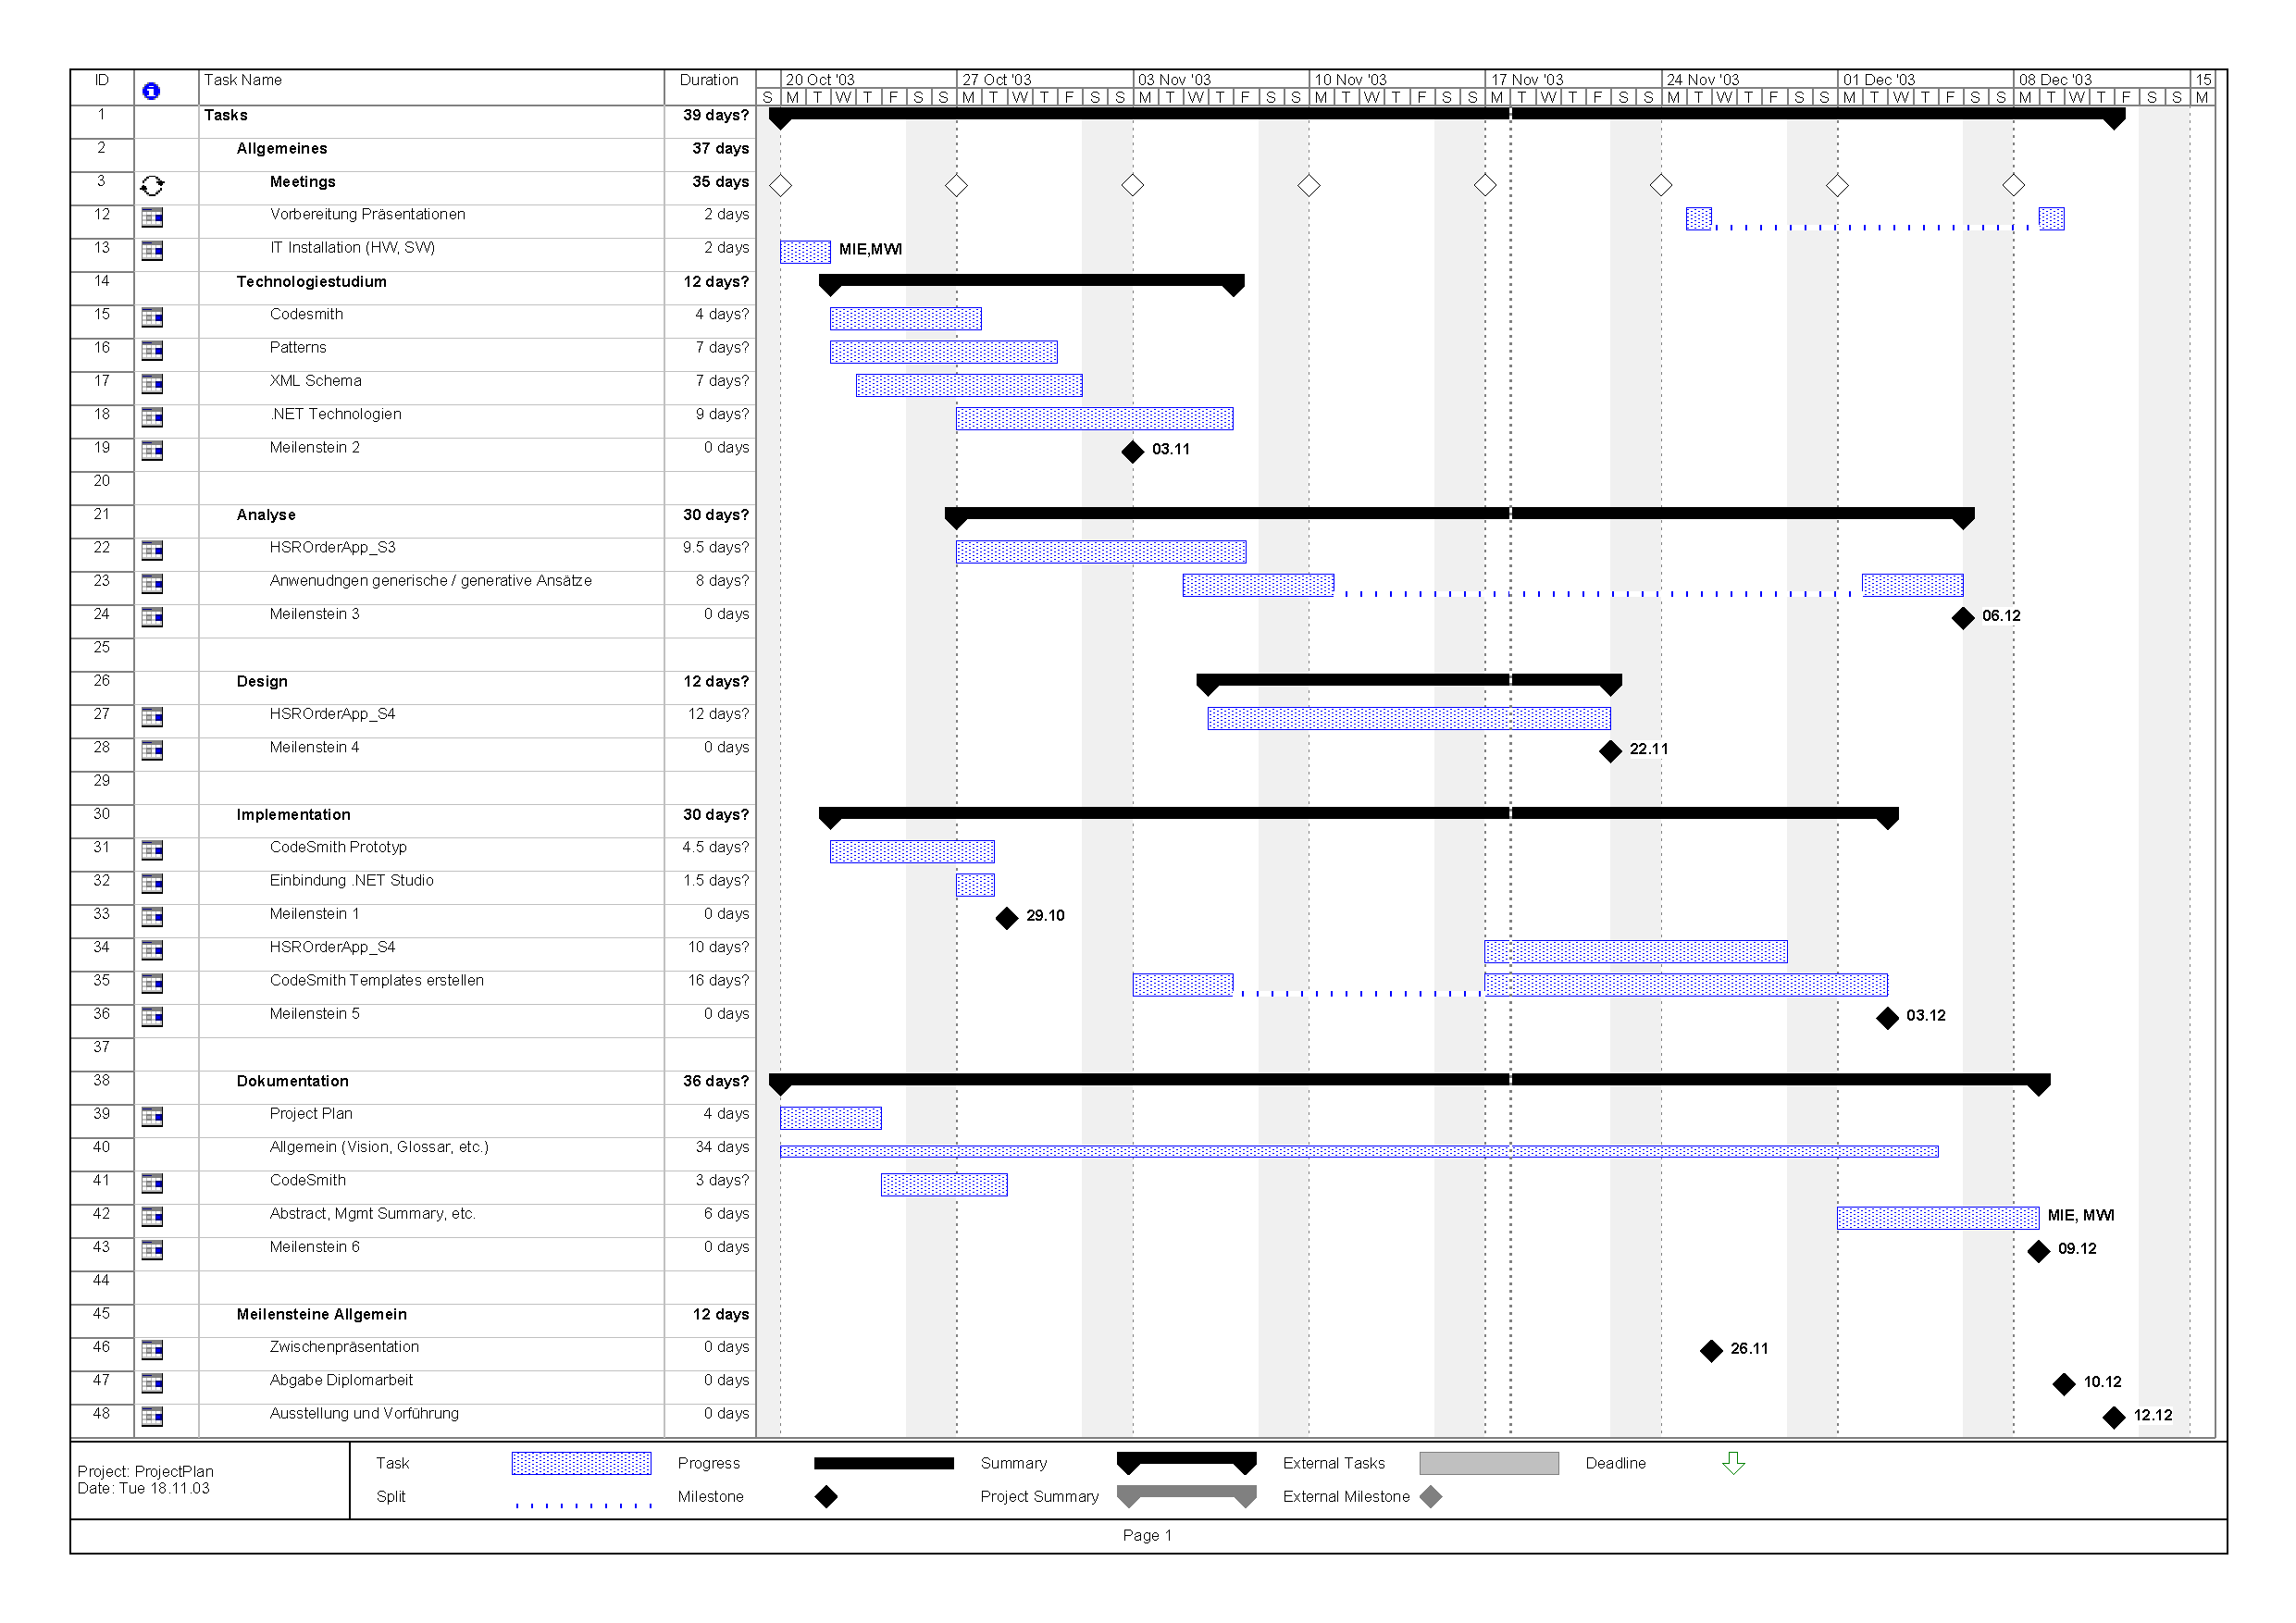
\includepdf[pages={1},landscape]{./files/inc/sources/ProjectPlan_v0-4}

		
	\section{�nderungsbeschreibung}
		\subsection{Version 0.2}
			F�r die CodeSmith Templates wurde sinnvollerweise ein eigener Task hinzugef�gt.
		\subsection{Version 0.3}
			Eine Dokumentation von Anwendungen der benutzten Patterns wird nicht ben�tigt. Erstens kann im
			Rahmen dieser zeitlich kurzen Arbeit nicht gen�gend Erfahrung mit verschiedenen Applikationen
			gesammelt werden, damit eine solche Dokumentation Sinn machen w�rde, und zweitens gibt es bereits
			viele B�cher bzw. Berichte die dieses Thema behandeln.
			
			Zudem werden schon fr�her als geplant erste CodeSmith Templates geschrieben, damit Risiken
			diesbez�glich minimiert werden k�nnen.
		\subsection{Version 0.4}
			Meilenstein 3 (siehe Beschreibung \hyperlink{milestone3}{Meilenstein 3}) wurde nach hinten verschoben. 
			Der Grund daf�r ist, dass es sich bei diesem Meilenstein um die
			Dokumentation von Erkenntnissen handelt, die wir erst am Schluss in vollem Umfange besitzen k�nnen.
			
			Der Task "`Templates erstellen"' wurde an die Implementation der HsrOrderApp\_S4 angepasst. Es hat sich
			gezeigt, dass es sinnvoll ist, wenn zuerst die Applikation von Hand geschrieben wird und erst anschliessend
			die entsprechenden Templates daf�r geschrieben werden. Das hat zu Konsequenz, dass die Templates erst
			nach der Implementation der Applikation fertig gestellt werden k�nnen.
	
\chapter{Zeitplanung}
	\section{Geplante Meilensteine}
		Es sind insgesamt 6 selbst definierte und 3 vorgegebene Meilensteine
		definiert. Die Meilensteine stimmen mit diesen im Projektplan �berein.
		Im Folgenden werden diese Meilensteine und deren Ziele erl�utert.
	
		\subsection{Selbst definierte Meilensteine}
			\begin{description}
				\item[Meilenstein 1]	Ein CodeSmith Prototyp wird erstellt. Dies beinhaltet
															die Einbindung eines Custom Tools in das Visual Studio
															.NET und die Generierung eines einfachen Codefiles aus der
															Definition einer XML Schema Datei. Zur Konfiguration soll
															eine XML Datei verwendet werden k�nnen, die direkt im Visual
															Studio .NET bearbeitet werden kann. Der Sinn dieses fr�h angesetzten 
															Meilensteins ist es, zeigen zu k�nnen, ob und wie mit dem Tool CodeSmith \cite{CodeSmith}
															die Ziele (namentlich die Codegenerierung f�r die HsrOrderApp\_S4)
															erreicht werden k�nnen. 
				\item[Meilenstein 2]	Das Technologiestudium von CodeSmith, XML Schema und der f�r diese
															Arbeit relevanten Patterns ist abgeschlossen. Das Studium der Patterns
															bezieht sich haupts�chlich auf das Lesen von B�chern, insbesondere
															die B�cher von M. Fowler \cite{Fowler03} und von E. Gamma \cite{Gamma97}.
															Nicht in diesem Meilenstein enthalten ist das Technologiestudium der
															.NET Technologien, da es w�hrend der Arbeit immer andere Technologien
															geben wird, in die man sich einarbeiten muss. Es gibt keine konkreten
															Resultate, die vorgewiesen werden. Der Meilenstein dient lediglich dazu,
															das n�tige Basiswissen bis zu diesem Zeitpunkt zu erarbeiten.
				\item[Meilenstein 3]	\hypertarget{milestone3}{}
															Die Analyse beinhaltet das Studium der bestehende HsrOrderApp\_S3, die 
															als Grundlage dieser Arbeit verwendet wird. Zudem wird eine Analyse
															gemacht, die zeigt, bei welchen Teilen einer Applikation es sinnvoll ist,
															generativ Code zu erzeugen und welche Patterns sich daf�r eignen.
															Aus diesen Erkenntnissen sollen m�gliche Vorschl�ge f�r Verbesserungen 
															gemacht werden, die in die HsrOrderApp\_S4 einfliessen.
														
															Aus jeder der genannten Analysen entsteht eine Dokumentation, die mit diesem
															Meilenstein abgeschlossen werden soll.
				\item[Meilenstein 4]	Aus der in Meilenstein 3 gewonnenen Erkenntnissen wird ein Design f�r die
															neu zu erstellende HsrOrderApp\_S4 gemacht. Das Design 
															wird mit diesem Meilenstein fertig gestellt.
				\item[Meilenstein 5]	Die Implementation teilt sich zeitlich in 2 verschiedene Bl�cke auf. Der 
															erste Block wird mit dem Meilenstein 1 abgeschlossen, der zweite wird mit 
															diesem Meilenstein abgeschlossen. Er umfasst die Implementation der HsrOrderApp\_S4
															und die Erstellung der CodeSmith Templates.
															Die HsrOrderApp\_S4 ist eine Erweiterung der HsrOrderApp\_S3 und soll mit Hilfe der 
															erstellten Templates erzeugt werden k�nnen.
				\item[Meilenstein 6]	Mit diesem Meilenstein wird die gesamte Dokumentation abgeschlossen. Vor
															allem beinhaltet dieser Meilenstein Dokumentation wie Management Summary, Abstract,
															Glossar, etc. Spezifische Teile der Dokumentation (wie z.B. eine Dokumentation
															zu CodeSmith) werden bereits in den korrespondierenden Phasen fertig gestellt
															und werden f�r diesen Meilenstein nur noch �berarbeitet.
			\end{description}
		
			\subsection{Vorgegebene Meilensteine}
			
				\begin{description}
					\item[Zwischenpr�sentation]	Die Zwischenpr�sentation dient der �berpr�fung der bis dahin 
																			erreichten Ziele. Um konkrete Resultate vorlegen zu k�nnen, sind die
																			selbst definierten Meilensteine mit dieses Meilenstein ab geglichen. Das 
																			bedeutet, dass bei der Zwischenpr�sentation Meilenstein 1 bis 4 fertig
																			gestellt wurden und bereits erste Resultate des Meilensteins 5 vorliegen 
																			sollten.
					\item[Abgabe Diplomarbeit]	Das eigentliche Ende der Diplomarbeit. An diesem Datum muss die Dokumentation
																			und die Implementation vollst�ndig abgeschlossen werden und die Resultate
																			dem Betreuer abgegeben werden.
					\item[Ausstellung und Vorf�hrung]
																			An diesem Tag findet eine �ffentliche Ausstellung der Diplomarbeiten statt.
																			Dazu m�ssen vorg�ngig Ausstellungs-Plakate erstellt werden und die Arbeitspl�tze 
																			werden f�r die Vorf�hrungen eingerichtet.
				\end{description}
				
	%----------
	\section{Erreichte Meilensteine}
		\subsection{Meilenstein 1}
			Dieser Meilenstein wurde Zeitgerecht fertig gestellt. Es wurde eine XML Schema Beschreibung erstellt,
			aus der ein Codefile generiert wurde. Zudem konnte es ebenfalls direkt aus dem Visual Studio .NET
			ausgef�hrt werden.
		\subsection{Meilenstein 2}
			Dieser Meilenstein wurde ebenfalls zeitgerecht erreicht. Wobei hierzu zu sagen ist, dass dieser
			Meilenstein eher virtueller Natur ist. Konkrete Resultate wurden hier nicht geliefert. Trotzdem
			haben wir uns bis dahin mit den Grundlegenden Technologien vertraut gemacht, was vor allem das
			Studium der Patterns und von XML Schema beinhaltete.
		\subsection{Meilenstein 3}
			Dieser Meilenstein ist etwas vage formuliert und aus diesem Grund schwierig einzustufen. Trotzdem
			haben wir bis zu diesem Meilenstein dessen Ziele erreicht. Die Ergebnisse waren eher implizit, da
			wenig konkrete Arbeiten daraus resultieren. Es war evtl. nicht sinnvoll, diesen Meilenstein �berhaupt
			zu definieren.
		\subsection{Meilenstein 4}
			Das Design wurde bis zu diesem Zeitpunkt gr�sstenteils fertiggestellt. Trotzdem haben wir
			auch nach diesem Meilenstein noch �nderungen vorgenommen. Der Grund daf�r ist, dass wir w�hrend
			den Tests noch Unsch�nheiten am Design feststellten. Trotz dieser �nderungen erachten
			wir diesen Meilenstein als erreicht.
		\subsection{Meilenstein 5}
			Die Implementation hat sich herausgez�gert. Dieser Termin war sehr optimistisch 
			angelegt. Wir haben ihn leider verpasst und haben auch in der letzten Woche noch implementiert.
			Dieser Teil der Implementation bezog sich aber vor allem auf die Tests. Mit dem Templates und
			der HsrOrderApp\_S4 waren wir zum Zeitpunkt dieses Meilensteins bereits fertig. Da unser
			Ziel aber war, die Implementationen vollst�ndig abzuschliessen, erachten wir diesen Meilenstein
			als nicht erreicht.
		\subsection{Meilenstein 6}
			Die Abgabe wurde eingehalten und somit ist der Meilenstein erreicht.
		
	%----------
	\section{Zeitaufstellung}
		Pro Woche sind $50h$ pro Person von der HSR vorgegeben. Dies entspricht
		einem totalen Pensum von $~ 750h$. Die folgende Tabelle fasst die 
		gesch�tzten und die tats�chlichen Stunden pro Kategorie zusammen. Die Stunden
		gelten jeweils als Total der von beiden Diplomanden aufgewendeten Stunden.
	
		\LTXtable{\linewidth}{./files/inc/tables/projektMgmtTime}
	
		\begin{figure}[htb]
			\begin{center}
				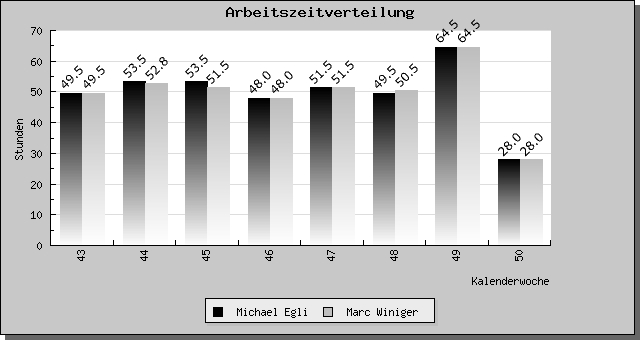
\includegraphics[width=\linewidth]{./files/inc/figures/pmZeit}
				\caption{\label{fig:pmZeit} Zeiterfassung}
			\end{center}
		\end{figure}
	
	%----------
	\section{Sitzungen}
		
		\subsection{Sitzung mit Betreuer}
		\begin{tabbing}
			\hspace*{2cm}\= \kill
			Wann:	\> W�chentlich, normalerweise montags.\\
			Wer:	\> H. Huser, M. Egli, M. Winiger\\
			Was:	\> Wochenziele definieren, Probleme besprechen.
		\end{tabbing}
		
		\subsection{Teamsitzung}
		\begin{tabbing}
			\hspace*{2cm}\= \kill
			Wann:	\> T�glich um 8.00 Uhr\\
			Wer:	\> M. Egli, M. Winiger\\
			Was:	\> Tagesziel definieren.
		\end{tabbing}
		
\chapter{Ressourcen}
\label{cha:ressourcen}
	\LTXtable{\linewidth}{./files/inc/tables/projektMgmtResources}

\part{Testbericht}
\label{par:testing}

\chapter{Ausgangslage}
	
	Getestet wurde die Funktionalit�t der HsrOrderApp\_S4. Da diese Applikation alle
	unterst�tzten F�lle der Code Generierung abdeckt, ist damit auch die Richtigkeit
	der Templates gew�hrleistet.

	\section{Testumgebung}
		Die Test wurden lokal ausgef�hrt und damit ist die Testumgebung dieselbe, wie
		in Kapitel \ref{cha:ressourcen} in der Tabelle \ref{tab:projektMgmtResources}
		angegeben wurde.
	
	\section{Datenbank}
		Das Design der Datenbank wurde vorgegeben. Es handelt sich dabei um die
		Datenbank f�r die HsrOrderApp. Diese wurde f�r die in dieser Arbeit
		erstellten Referenzimplementation verwendet und dient auch als Datenbank f�r 
		die Tests.

\chapter{HsrOrderApp\_S4}
	Wir haben entschieden, die bestehenden Tests der HsrOrderApp\_S3 zu erweitern. 
	Dazu haben wir Facade, WebServices, TestProxy und TestApplikation �bernommen 
	und an unsere Architektur angepasst.

	Getestet wurde damit der generierte Code der Domain Object und der Mapper.
	
	\section{Anforderungen an die Applikation}
	\begin{itemize}
		\item Neue Objekte
				
			Objekte �ber die Factory erstellen und in der UnitOfWork als new markieren.
		
		\item Objekte �ndern
		
			Geladene Objekte ver�ndern und in der UnitOfWork als dirty markieren.
		
		\item Objekte in die Datenbank schreiben
		
			Neue Objekte in die Datenbank einf�gen und ge�nderte Objekte in der Datenbank 
			auf den neusten Stand bringen.
		
		\item Objekte aus der Datenbank lesen
		
			Die Daten f�r neu zu erstellende Objekte werden mittels find Methoden aus der 
			Datenbank geholt.
		
		\item Objekte als gel�scht markieren
		
			Objekte f�r das l�schen in der Datenbank bei der UnitOfWork registrieren.
		
		\item Rekursives L�schen
		
			Wird ein Objekt mit ToMany Relationen gel�scht, m�ssen alle zugeordneten 
			Objekte vorher auch gel�scht werden.
				
		\item Werfen von Concurrency Exceptions
		
			Werden versucht veraltete Objekte auf die Datenbank zu schreiben, muss eine 
			Concurrency Exception geworfen werden.
		
	\end{itemize}
	
	\section{Durchgef�hrte Tests}
		Die folgenden drei Test werden mehrmals hintereinander ausgef�hrt. Zuerst werden 
		jeweils die in der letzen Iteration erstellten Objekte gesucht und wenn vorhanden 
		gel�scht. Objekte einer ToMany Relation m�ssen von den Mappern automatisch gel�scht
		werden. Das dies auch wirklich geschieht, wird durch Constraints auf der Datenbank 
		�berpr�ft.
	
		\subsection{Person Test}
			Es werden drei neue Personen Objekte erstellt. Zu jeder Person werden zwei 
			Adressen erstellt. Diese werden in die Datenbank geschrieben.
			
			Danach werden die Personen Objekte ge�ndert, je eine zus�tzliche Adresse 
			hinzugef�gt und ebenfalls in die Datenbank geschrieben.
		
		\subsection{Product Test}
			Es werden 16 Produkte Objekte in vier Kategorien erstellt und auf die Datenbank 
			geschrieben.
		
			Davon werden 12 Objekte ver�ndert und 4 Objekte wieder gel�scht. Diese Operationen 
			werden in einem Schritt auf der Datenbank ausgef�hrt.
			
		\subsection{Order Test}
			Die Personen und Produkte aus den vorherigen Tests werden �ber die Finder Methoden
			gesucht.
			
			Der ersten Person werden drei Bestellungen mit je drei Positionen hinzugef�gt. 
			Diese �nderungen werden auf die Datenbank geschrieben. Danach werden die Positionen 
			ge�ndert, hinzugef�gt und gel�scht.
	
	\section{Ergebnisse}
		Die Tests laufen ohne Fehler durch. Der Trace vom SQL Profiler und eine Kontrolle in 
		der Datenbank belegen, dass die Eintr�ge auch wirklich geschrieben wurden.
		
		Werden w�hrend den laufenden Tests die Datenbank-Eintr�ge ver�ndert, sollte eine Concurrency Exception geworfen werden. 
		Die Applikation st�rzt jedoch einer NullReferenzeException ab. Nach beheben dieses Fehlers reagiert alles wie erwartet.



%%anhang als Text im kolumnetitel
\renewcommand{\chaptermark}[1]{%
\markboth{\appendixname\ \thechapter{}: #1}{}}
\renewcommand{\sectionmark}[1]{%
\markright{\thesection{}: #1}{}}

%fix appendix bookmarks
\pdfbookmark[-1]{Appendix}{\appendixname}

%\selectlanguage{english}
\begin{appendix}
\selectlanguage{ngerman}
	\chapter{Pers�nliche Berichte}

	\section{Michael Egli}
		Im Nachhinein kann muss ich sagen, dass dieses Projekt in vielen Hinsichten sehr spannend war.
		Zu Beginn war ich zwar etwas skeptisch, das hat sich aber schon bald in Interesse f�r das
		Projekt gewandelt. Das Spannende am Projekt f�r mich war, dass es sehr viele technische Aspekte
		tangierte. Zum Einen war dies XML und XML Schema, zum Anderen aber auch generische
		und generative Programmierung. Ebenfalls spannend war die pattern-orientierte Entwicklung.
		F�r mich war es das erste Projekt, bei dem ich so intensiv Patterns verwendet habe.
		
		Leider muss man sagen, dass wir sehr viele Stunden mit CodeSmith verbracht haben. Das Tool
		ist sehr schlecht dokumentiert und es funktioniert auch nicht alles, wie wir es erwartet
		haben.
		
		F�r mich ist das Resultat der Arbeit sehr erfreulich. Ich glaube wir k�nnen mit
		\textit{STORM} einen guten L�sungsansatz f�r das gestellte Problem pr�sentieren.
		Nat�rlich w�re es ausbauf�hig, aber die Zeit war leider sehr knapp daf�r.
		
		Das Projekt war �ber das Ganze gesehen sehr denklastig, was ich als positiv bewerte. Wir
		mussten uns sehr oft genau �berlegen, wie wir ein Problem l�sen k�nnen.
		
		Die Zusammenarbeit mit Marc kannte ich schon aus der letzten Semesterarbeit. Obwohl die
		Zeit w�hrend der Diplomarbeit sehr anstrengend war, hat die Teamarbeit immer funktioniert.
		Ich denke, dass wir uns sehr gut erg�nzt haben und auch, dass wir es geschafft haben die
		St�rken von beiden gut auszunutzen.
		
		Die Betreuung fand ich sehr gut. Zum Einen hatten wir Betreuung von Herrn Huser, zum
		Anderen auch noch von M. Konrad. Dies hat mich positiv �berrascht und hat uns auch 
		sehr oft geholfen. Es w�re sch�n, wenn es immer so w�re, aber leider haben wir 
		in fr�heren Projekten auch schon Anderes erlebt.
		
		Zusammenfassend kann ich sagen, dass ich sehr viel gelernt habe. Vor allem auch Dinge
		wie generative Programmierung, die ich unter Umst�nden in Zukunft gut gebrauchen kann.
		
		
	\section{Marc Winiger}
		Kurz vor Beginn der Diplomarbeit wurde das urspr�nglich geplante Thema verworfen. 
		Das neue Thema war generative Programmierung. Zuerst war ich eher skeptisch, denn 
		bisher habe ich immer wenn ich etwas Entwickelt habe, versucht das Problem so 
		generisch wie M�glich zu l�sen. Die generative Programmierung war f�r mich also 
		ein ganz neuer Aspekt.
		
		Es ist nicht einfach sich in Code einzuarbeiten, der von jemand anderem entwickelt 
		wurde. Das Ziel war es die existierende HsrOrderApp umzubauen und Teile davon mit 
		generiertem Code zu ersetzen. Beim �ndern einer existierenden Applikation, kann nach 
		unseren Erfahrungen sehr viel Zeit verloren gehen. Nach den negativen Erfahrungen der 
		letzen Semesterarbeit, bin ich froh, dass wir die M�glichkeit hatten, ein eigenes 
		Projekt zu starten und zu einem sp�teren Zeitpunkt die noch fehlenden Teile von der 
		existierenden Applikation zu �bernehmen. So hatten wir relativ schnell einen 
		Funktionierenden Prototypen. 
		
		Im Laufe des Projekt habe ich immer mehr Gefallen an der gerativen Programmierung 
		gefunden. Denn es ist zwar ein grosser Aufwand ein Template zu schreiben, das alle 
		F�lle abdeckt und auch noch fehlerfreien Code erzeugt. Doch wenn man das erst mal 
		gemacht hat, ist es genial, wenn man nur noch eine einfache Beschreibung braucht aus 
		denen dann hunderte Zeilen Code generiert werden.
		
		Obwohl wir am Anfang mit dem L�sungsansatz XML Schema theoretisch etwas Zeit verloren 
		haben, habe ich es interessant gefunden verschiedene Wege zu sehen, wie die Generierung 
		des Codes konfiguriert werden kann.
		
		Nachdem ich bereits bei der letzen Semesterarbeit mit Michael zusammen gearbeitet habe, 
		war f�r mich klar, dass ich auch die Diplomarbeit mit ihm durchstehen m�chte. Es sind 
		acht Wochen, in denen man sehr viel Zeit miteinander verbringt. Trotzdem hatten wir nie 
		ernsthafte Auseinandersetzungen. Ich w�rde mit ihm sofort wieder ein Projekt angehen.
		
		Es waren acht doch ziemlich strenge Wochen auf die wir zur�ckblicken k�nnen. Doch da wir 
		von Anfang ein Ziel vor Augen hatten, war es immer m�glich, sich irgendwie zu motivieren. 
		Alles in allem muss ich sagen dass es eine sch�ne, interessante und auch lehrreiche Zeit 
		war.
		
	\chapter{Protokolle}

\section{Sitzung 1 vom 20. Oktober 2003}

\subsection{Teilnehmer}
H. Huser (hhu), M. Egli (meg), M. Winiger (mwi)

\subsection{Themen}
	\begin{itemize}
		\item Besprechung Aufgabenstellung
		\item Allgemeine Fragen zum Projektstart
	\end{itemize}
\subsection{Aufgabenstellung}
	Die Aufgabenstellung ist noch nicht fix. Es ist m�glich, dass im Verlauf der Arbeit noch Verschiebungen der
	erwarteten Resultate m�glich sind.

\subsection{Entscheidungen}
\begin{itemize}
	\item Der Projektplan muss versioniert werden, damit �nderungen w�hrend dem Projekt auch im
	Nachhinein ersichtlich sind.
	\item Wir setzen eine Online-Zeiterfassung ein. Die Beschreibung zu den Eintr�gen dient
	gleichzeitig als Projekt-Tagebuch.\\
	\url{http://homer.skymx.net/zeit/ooxgen/}
	\item Wir w�rden die Dokumentation gerne mit \LaTeX{} erstellen. Wir versuchen eine L�sung zu finden, dass wir
	die Dokumentation, bzw. einzelne Dokumente davon, in ein zu Microsoft Word kompatibles Format umwandeln k�nnen.
	\item Einzelne Dokumente (z.B. Technischer Bericht) werden in Englisch verfasst.
\end{itemize}

\subsection{Hinweise}
	\begin{itemize}
		\item (hhu): Auf der MSDN Seite finden wir Pattern von Microsoft, die f�r uns n�tzlich sein
		k�nnten.\\
		\url{http://msdn.microsoft.com/architecture/patterns/MSpatterns/}\\
		\url{http://msdn.microsoft.com/architecture/application/default.aspx?pull=/library/en-us/dnbda/html/distapp.asp}
		\item (hhu): Der erwartete Einsatz f�r die Diplomarbeit liegt bei 50h/Woche.
	\end{itemize}
	
\subsection{Ziele}
\begin{itemize}
	\item Erstellen des Projektplans, damit dieser an der n�chsten Sitzung besprochen werden kann.
	\item Einarbeiten in HsrOrderApp\_S3
	\item Vertiefung von Pattern und .NET Technologien
\end{itemize}

\newpage

\section{Sitzung 2 vom 28. Oktober 2003}

\subsection{Teilnehmer}
H. Huser (hhu), M. Egli (meg), M. Winiger (mwi)

\subsection{Themen}
	\begin{itemize}
	  \item Wochenr�ckblick
		\item Projektplan v1.0
		\item Dokumentation
	\end{itemize}

\subsection{Wochenr�ckblick}
\begin{itemize}
  \item Der Projektplan (v0.1) liegt vor und die Meilensteine sind in der Doku
    beschrieben.
  \item Die Technologiestudien Patterns und CodeSmith sind gr�sstenteils
    abgeschlossen.
\end{itemize}

\subsection{Projektplan v0.1}
Der Projektplan ist soweit in Ordnung. Die Planung ist f�r uns nicht einfach, da
wir uns zuerst mit den Technologien und Patterns vertraut machen m�ssen. Wichtig
ist, dass wir auftretende �nderungen am Projektplan sofort mit (hhu) besprechen.

\subsection{Dokumentation}
	\begin{description}
		\item[Risikoanalyse]
		  Zu allgemein. Konkretere L�sungen m�ssen angegeben werden.
		\item[Meilenstein 3]
		  Das Ziel ist zu hoch angesetzt. Es reicht wenn wir zeigen
		  welche Art von Mappings durch generativen Code ersetzt werden k�nnen.
		\item[Implementation]
		  Die Erstellung der Templates, welche als Werkzeuge
		  eingesetzt werden k�nnen, sollten in der Planung von der Implementation der
		  Beispiel-Applikation (HsrOrderApp\_S4) getrennt werden.
		\item[Bibliographie]
		  Die MSDN Architecture Patterns von Microsoft sollten in die
		  Bibliographie aufgenommen werden.
		\item[Allgemein]
		  Wir generieren aus dem Technical Report ein eigenst�ndiges
		  Dokument.
	\end{description}

\newpage

\section{Sitzung 3 vom 3. November 2003}


%-----
\subsection{Teilnehmer}
H. Huser (hhu), M. Egli (meg), M. Winiger (mwi)


%-----
\subsection{Themen}
	\begin{itemize}
		\item Anforderungs-Spezifikation
		\item Technischer Bericht
		\item Weiteres Vorgehen
	\end{itemize}


%-----
\subsection{Anforderungs-Spezifikation}

\noindent Q: Es gibt unsererseits Unklarheiten bez�glich dem Verfassen einer 
Anforderungs-Spezifikation.

\noindent A: Vor allem im ersten Teil der Arbeit geht es darum die bestehende 
Applikation zu analysieren. Wir m�ssen L�sungsans�tze suchen 
und herausfinden was die beste L�sung ist. Darum werden sich 
Anforderungen erst im Verlaufe des Projekt ergeben.
	
%-----
\subsection{Technischer Bericht}

Der erste Teil des technischen Berichts liegt vor. Es handelt sich 
dabei um eine Zusammenfassung der f�r unser Projekt wichtigen 
Pattern aus dem Buch von Fowler \cite{Fowler03} und einer 
kurzen Beschreibung zu CodeSmith \cite{CodeSmith}.

Wir werden das PDF auf \url{http://ooxgen.linda.homelinux.net/} 
laden und w�rden gerne an der n�chsten Sitzung ein Feedback erhalten.


%-----
\subsection{Weiteres Vorgehen}

Die Analyse der bestehenden Applikation, die Erstellung von Templates	
und das Dokumentieren der Erkenntnisse erfolgt im Moment fast 
gleichzeitig. Anfangs Woche werden wir den Schwerpunkt auf die 
Spezifikation der XML Schemas und das programmieren des zum parsen 
ben�tigten Code setzen. 


\newpage

\section{Sitzung 4 vom 12. November 2003}


%-----
\subsection{Teilnehmer}
H. Huser (hhu), M. Egli (meg), M. Winiger (mwi)


%-----
\subsection{Themen}
	\begin{itemize}
		\item Lebensdauer von Objekten
		\item Doku
		\item Planung/Fortschritt
	\end{itemize}


%-----
\subsection{Lebensdauer von Objekten}
Es m�ssen verschiedene Fragen bez�glich Lebensdauer der Objekte angeschaut 
werden.

Ist es besser wenn die Objekte nach einem Commit zerst�rt werden, 
oder k�nnen sie evtl. sp�ter wieder verwendet werden? Wird die Konsitenz 
bei Objekten aus der IdentitiyMap �berpr�ft? K�nnen die Objekte eingeteilt 
werden in eher statische Daten und solche, die man jedesmal neu von der 
Datenbank holen muss? Soll die Wahl zwischen Geschwindigkeit und Aktualit�t 
dem Benutzer �berlassen werden?

%-----
\subsection{Doku}
Wir haben die beiden Technologien XML Schema und Reflection im Vergleich 
dokumentiert. Wir m�ssen den Teil noch �berarbeiten und werden ihn vor der 
n�chsten Sitzung mailen.

%-----
\subsection{Planung/Fortschritt}
CodeSmith bereitet uns immer wieder Schwierigkeiten, weil vieles nicht 
gerade auf Anhieb funktioniert. Wir haben etwas fr�her mit der 
Implementation einer neuen HsrOrderApp begonnen und sind jetzt an den 
ersten Versuchen die Templates einzubauen.
\newpage

\section{Sitzung 5 vom 18. November 2003}


%-----
\subsection{Teilnehmer}
H. Huser (hhu), M. Egli (meg), M. Winiger (mwi)


%-----
\subsection{Themen}
	\begin{itemize}
		\item Generischer/generativer Ansatz
		\item Enums, Lookup-Tables
	\end{itemize}


%-----
\subsection{Generischer/generativer Ansatz}

Es zeigt sich, dass der generative Ansatz viel aufwendiger 
zu realisieren ist, als am Anfang angenommen. Es gibt sehr 
viele Spezialf�lle. Eine Applikation wie die HsrOrderApp 
ist zu klein, dass sich der ernsthafte Einsatz von 
Code-Generierung lohnen w�rde.


%-----
\subsection{Enums, Lookup-Tables}

Enums sind einer dieser Spezialf�lle. Es gibt verschiedene 
M�glichkeiten diese auf die Datenbank zu mappen. Eine 
M�glichkeit w�ren Lookup-Tables. Dabei werden die 
Enum-Beschreibungen, mit eindeutigen IDs, in einzelnen oder 
einer gemeinsamen Tabelle abgelegt.

Eine entscheidende Rolle spielt f�r den Mapping-Code, wie 
die Enums in der Datenbank abgelegt sind. Liegt ein 
unver�nderbares Datenbank-Schema vor, muss der Code mit 
grosser Wahrscheinlichkeit spezifisch geschrieben werden.

Abgesehen davon werden die Enums in der HsrOderApp-Datenbank 
nicht sehr sch�n abgelegt. Sie sind nicht vollst�ndig 
normalisiert und somit redundant als VARCHAR abgelegt, was 
das mapping noch ein St�ck komplizierter macht

\newpage

\section{Sitzung 6 vom 24. November 2003}


%-----
\subsection{Teilnehmer}
H. Huser (hhu), M. Egli (meg), M. Winiger (mwi)


%-----
\subsection{Themen}
	\begin{itemize}
		\item Projektstand
		\item Zwischenpr�sentation
	\end{itemize}


%-----
\subsection{Projektstand}
Domain-Objekte k�nnen bereits kompilierbar mit den Templates generiert 
werden. Die Templates f�r die Mapper sollten auch bald soweit sein.

Die Templates sind so geschrieben, dass Primary Keys auch �ber mehrere 
Kolonnen definiert sein k�nnen. Das hat zum Teil etwas mehr Zeit ben�tigt
als erwartet. Es w�re einfacher gewesen nur Surrogate Keys zu behandeln.
Wir haben jetzt jedoch schon �berall mehrteilige Keys verwendet.


%-----
\subsection{Zwischenpr�sentation}
Am Mittwoch 26. November um 15.00 Uhr findet eine Sitzung mit Hr. B�rfuss 
statt. Wir erkl�ren den verwendeten Ansatz mit Attributierung und Reflection 
und pr�sentieren was wir bisher gemacht haben. Ausserdem sollten wir unsere 
Erkenntnisse aufzeigen.

Wir erstellen einen aktualisierten Projektplan bis Mittwoch.

%	\input{./files/tools}
%\selectlanguage{english}
	%%Bitte beim eintragen alphabetisch ordnen
\chapter{Glossary}

\begin{description}

\item[\Large{A}]
	\hypertarget{assembly}{}
	\item[assembly] A collection of one or more files that are versioned and deployed as a unit. 
									An assembly is the primary building block of a .NET Framework application. 
									All managed types and resources are contained within an assembly and are 
									marked either as accessible only within the assembly or as accessible from 
									code in other assemblies.

	\item[attribute] A .NET class used to describe code elements. This attributes can be read by reflection on runtime.

\item[\Large{C}]
	\item[CodeSmith] A freeware template-based code generator.

\item[\Large{D}]
	\item[DLL] ``Dynamic Link Library'' in .NET is an \hyperlink{assembly}{assembly}.

\item[\Large{G}]
	\item[GAC] ``Global Assembly Cache'' is the place where .NET Assembliesy can be registred. The 
	           Assembly needs to be signed. It is possible to register different Versions of the 
	           same Assembly.

\item[\Large{I}]
	\item[IDE] ``Integrated Developing Environment'' is a tool for developers. Such as Visual Studio .NET.

\item[\Large{M}]
	\item[makefile] File with a description of a build process. It defines dependencies between several tasks. Nmake is the .NET tool to execute the file.
	\item[mapper] An object-relational mapper maps the data from an object to a table on the database and vice versa.
	
\item[\Large{P}]
	\item[primary key] The primary key of a relational table uniquely identifies each record in the table. 
	It can either be a normal attribute that is guaranteed to be unique or it can be generated by the database.

\item[\Large{R}]
	\item[reflection] A mechanism to get information about running code.

\item[\Large{T}]
	\item[transaction] An inseparable list of database operations which must be executed either in its entirety or not at all.
	
\item[\Large{X}]
	\item[XML Schema Definition (XSD)] specifies how to formally describe the elements in an XML document. This description can be used to verify that each item of content in a document adheres to the description of the element in which the content is to be placed.

\end{description}

	\bibliography{./files/inc/references}
%	\printindex
\end{appendix}

\end{document}
